% For twosided version:
% - change oneside in class options to twoside
% - change margins to two sided version in ueathesis.sty
% - change fancy headings to two sided version in ueathesis.sty
% - save ueathesis.sty and rebuild this file

\documentclass[11pt,twoside]{ueathesis}
\usepackage{ueathesis}
\usepackage{csquotes}
\usepackage{epigraph}
\usepackage{booktabs}
\usepackage{listings}
\lstset{
    basicstyle=\ttfamily\footnotesize,
    breaklines=true
}
\usepackage{syntax}

\usepackage{graphicx} % Required for inserting images
\usepackage{svg}

\usepackage[nonumberlist,toc]{glossaries}
%\makeglossaries[title=Glossary, toctitle=Glossary]
\makeglossaries

\usepackage{framed}
% for annotations such as boxes and bars round te

% includes to help deal with problem characters in urls
\usepackage[strings]{underscore}
\usepackage{url}

\usepackage{silence}
\WarningsOff[everypage]% Suppress warnings related to package everypage

\usepackage{datetime}
\newdateformat{universaldate}{\THEYEAR-\twodigit{\THEMONTH}-\twodigit{\THEDAY}}

\usepackage{longtable}
\usepackage{tablefootnote} % supoport footnotes in tables
\usepackage{makecell} % support splitting lines in tables

\hypersetup{
    hidelinks,
    colorlinks=false,
}

\newcommand\appref[1]{Appendix \ref{#1}}
\usepackage{cleveref}

\newcommand{\DocTitle}{Sustainable Software Systems: An investigation into comparing the performance and energy consumption of software components}
\newcommand{\AuthorName}{Francis Kenneth Carver}
\newcommand{\SubmissionMonth}{March}
\newcommand{\SubmissionYear}{2024}

\setcounter{secnumdepth}{3}
\setcounter{tocdepth}{3}

\def\subsectionautorefname{Section}
\def\subsubsectionautorefname{Section}

\renewcommand\floatpagefraction{0} %default 0.5

\makeatletter
\newcommand\subsubsubsection{\@startsection{paragraph}{4}{\z@}{-2.5ex\@plus -1ex \@minus -.25ex}{1.25ex \@plus .25ex}{\normalfont\normalsize\bfseries}}
% \newcommand\subsubsubsubsection{\@startsection{subparagraph}{5}{\z@}{-2.5ex\@plus -1ex \@minus -.25ex}{1.25ex \@plus .25ex}{\normalfont\normalsize\bfseries}}
\makeatother

\makeatletter
\newcommand{\verbatimfont}[1]{\renewcommand{\verbatim@font}{\ttfamily#1}}
\makeatother

\makeatletter
\renewcommand*\l@figure{\@dottedtocline{1}{1em}{3.2em}}
\makeatother

\BeforeBeginEnvironment{verbatim}{\def\baselinestretch{1}}

\citetrackerfalse

\begin{document}

\pagenumbering{gobble}
%%%%%%%%%%%%
%
% UEAThesisFrontMatter
% A .tex template for front matter that conforms to the UEA thesis guidelines 
% (see: https://portal.uea.ac.uk/documents/6207125/6873036/Section%2B3%2BTheses%2BNEW/69d413a9-8639-41d5-8fc2-b391b1a4bfb9)
% 
% Version 1.0.1
% 
% Compiled by Tom Coleman and Dane Grundy, with thanks to Robert Whittaker for LaTeX knowledge and the UEA PGR office for command suggestions
%
% Questions, comments, bugs? Email either d.grundy@uea.ac.uk, danegrundy@googlemail.com or tdhc@st-andrews.ac.uk
%
% CC Attribution 4.0 International  (https://creativecommons.org/licenses/by/4.0/)
%
%%%%%%%%%%%% 
%
% To use: \include this document inside a .tex file with \documentclass{book} (or \documentclass{ueathesis}) and \usepackage{ueathesis}, just after \begin{document}.
%
% The sequencing of material in this section is defined by UEA thesis guidelines 2. (9) xiii). Please do not change.
%
%%%%%%%%%%%%

%%%%%%%%%%%%
%
% Title page
%
%%%%%%%%%%%%


\thispagestyle{empty}
\begin{titlepage}
\begin{center}
\hrule
\vspace{1.5em}
\Huge\textbf{\DocTitle}\par
\vspace{1em}
\hrule
\vspace{0.5in}

\Large{A thesis submitted to the School of Computing Sciences at the University of East Anglia in partial fulfilment of the requirements for the degree of Doctor of Philosophy}\par

\vspace{0.5in}

\LARGE{\AuthorName\\ \Large{\SubmissionMonth\ \SubmissionYear}}\par
\vspace{0.2in}
\end{center}

% Copyright disclaimer: required by UEA thesis guidelines 2. (1).

\textcopyright{2024} This copy of the thesis has been supplied on condition that anyone who consults it is understood to recognise 
that its copyright rests with the author and that use of any information derived there from must be in accordance 
with current UK Copyright Law. In addition, any quotation or extract must include full attribution.

\end{titlepage}
%\afterpage{\null\newpage}
%\thispagestyle{empty}

%%%%%%%%%%%%
%
% Abstract % This should be fewer than 300 words on no more than one side of A4 paper, by UEA thesis guidelines.
%
%%%%%%%%%%%%

\newpage
\thispagestyle{empty}
\chapter*{Abstract}
\label{chapter:abstract}
\phantomsection\addcontentsline{toc}{chapter}{Abstract}

Information and communication technologies (ICT) are an increasing contributor to greenhouse gas emissions, but ICT systems are a combination of hardware and software. Hardware is the part that requires raw materials and manufacturing processes, consumes electricity, and generates heat when in use. However, in most cases, this hardware is only present in order to run application software. Changing or replacing that software can affect both the amount of hardware needed and the resources consumed during its operation. Although ICT systems have the potential to improve the sustainability of other fields, improving the sustainability of the ICT systems themselves is a vital undertaking.

Modern software is typically constructed by combining and reusing other software in the form of libraries and components. Selecting these components is a key aspect of software development. The design and construction of ICT systems is subject to conflicting economic, practical, technological, and political constraints. Historically, the environmental impact of software development choices has had a much lower priority than economic or functional factors. Software developers face a confusing array of choices and a lack of reliable information with which to make decisions. A series of studies were conducted to determine the practicality and impact of replacing software components with functionally equivalent alternatives.

A representative category of components was chosen and the performance of a selection of components was compared to determine whether selecting more performant components could reduce hardware requirements. The results of the performance measurements showed that the fastest component in the selected group was, on average, 2642 times faster than the slowest. The implication of this is that the selection and substitution of components can potentially have a large impact on the performance, and therefore the hardware requirements, of a large-scale system.

A prototype apparatus was developed to measure the energy consumption of software in operation. This apparatus revealed that the popular WordPress website management software consumes considerably more energy in operation than an equivalent static website. The implication of this is that for many websites, moving from WordPress to a static website could result in immediate energy savings.

The apparatus was also used to compare the energy use of the class of components examined in the performance tests. This comparison showed that energy usage is not directly related to software performance and that different components have different energy usage profiles under different usage scenarios. The implication of this is that performance alone should not be used to predict energy use and that the most accurate way to determine the energy impact of a software change is to include energy measurements in existing test suites.

This dissertation is the result of my own work and includes nothing that is the result of work done in collaboration except where specifically indicated in the text.

%%%%%%%%%%%%
%
% Table of contents
%
%%%%%%%%%%%%

\newpage
\thispagestyle{empty}
\tableofcontents

%%%%%%%%%%%%
%
% List of figures
%
%%%%%%%%%%%%

% If no figures, comment out

\cleardoublepage
\phantomsection
\addcontentsline{toc}{chapter}{\listfigurename}
\listoffigures

%%%%%%%%%%%%
%
% List of tables
%
%%%%%%%%%%%%

% If no tables, comment out

\cleardoublepage
\phantomsection
\addcontentsline{toc}{chapter}{\listtablename}
\listoftables

%%%%%%%%%%%%
%
% List of listings
%
%%%%%%%%%%%%

% If no listings, comment out

\cleardoublepage
\phantomsection
\addcontentsline{toc}{chapter}{List of Code Listings}
\lstlistoflistings

%%%%%%%%%%%%
%
% Acknowledgements + dedications
%
%%%%%%%%%%%%

\chapter*{Acknowledgements}
\label{chapter:acknowledgements}
\addcontentsline{toc}{chapter}{Acknowledgements}

Above all, endless thanks to my wife Margaret and my daughters Elizabeth and Katherine for putting up with this unexpectedly lengthy process and the associated plunge in family income.

Special thanks to Professor Nicholas Caldwell for his continuing support and for remaining professional while juggling the sometimes conflicting demands of being both PhD supervisor and line manager.

And finally, thanks to all my friends and colleagues who have helped out with suggestions, encouragement, comments, critiques, feedback and opportunities to discuss and publicise my work.


\thispagestyle{empty}
\newpage
\thispagestyle{empty}

%\chapter*{Dedications}
%\addcontentsline{toc}{chapter}{Dedications}


\clearpage
\pagenumbering{arabic}

\raggedbottom

\chapter{Introduction}
\label{chapter:introduction}

\section{About This Research}
\label{section:intro about}

\begin{leftbar}
This research is motivated by concern for the future of our environment.
\end{leftbar}

The world is facing an environmental crisis, and all organisations and individuals need to play their part in addressing climate change. We have already overstepped key planetary boundaries \citep{Steffen2015} and continue to cause irreversible problems. The longer we delay in reducing carbon emissions to zero, the greater the cumulative impact on the world \citep{Pierrehumbert2019}.

\begin{leftbar}
This research is situated in the area of sustainability.
\end{leftbar}

The climate crisis and the environmental impact of humanity are aspects of sustainability, but sustainability itself can be a controversial concept. The literature is full of definitions of sustainability. A popular introductory approach is to describe sustainability as the ability or capability to \enquote{endure} \citep{Mengesha2024}, \citep{Dixit2024}, \citep{Venters2023}, and many others. Although this definition may be correct from a dictionary perspective, it does not align well with common usage and is open to misunderstanding about \emph{what}, exactly, should endure. Another commonly cited definition is from \citet{Brundtland1987} \enquote{meeting the needs of the present generation while not compromising the ability of future generations to meet their needs}. However, \citet{Owens2003} describes this definition as leading to a \enquote{striking paradox} with the quest for sustainability being neither a \enquote{consensual} nor a \enquote{straightforward} project. In \citeyear{Allen1993}, \citeauthor{Allen1993} described sustainability as \enquote{an immature notion} that \enquote{conjures up different images} in different readers. More recently \citet{Moore2017} lists \enquote{lack of consistent definitions in the literature} as one of the major challenges of research involving sustainability, finding 24 separate definitions in a survey of 209 articles. In \citeyear{UnitedNations2015}, \citeauthor{UnitedNations2015} defined a set of 17 \emph{Sustainable Development Goals} (\autoref{17-goals-image}) that have become a baseline for categorising research. The mapping of this research to the United Nations Sustainable Development Goals is given in \autoref{section:un goals}.

In this dissertation, \emph{environment} is used to refer to the natural environment, and \emph{sustainability} is used in the sense of minimising environmental, especially climate, impact.

\begin{leftbar}
This research considers the sustainability of Information and Communication Technology (\gls{ICT}).
\end{leftbar}

\label{A4} \label{A6}
\gls{ICT} is important because it participates on both sides of the metaphorical \gls{sustainability ledger}. \gls{ICT} can provide assistance and solutions to increase the sustainability of a wide range of processes. However, \gls{ICT} systems also consume resources and energy to manufacture, distribute, operate and dispose of. \gls{ICT} systems can help in any of the \gls{un goals}, for example by reducing travel through virtual meetings, calculating fuel-efficient delivery routes, or controlling agricultural machinery for greater crop yields. However, the manufacturing, operation, and disposal of such systems have a large environmental cost. 

\label{E8}
At the start of this research, estimates showed that the \gls{ICT} sector contributed between 1.8\% and 5\% of the total greenhouse gas emissions worldwide, depending on the model used \citep{Belkhir2018}. To put this into perspective, the higher end of \citeauthor{Belkhir2018}'s estimates proportion is roughly twice the emissions due to air travel over the same period. Despite high-profile climate pledges, this contribution has not decreased. With the progressive adoption of energy-intensive technologies such as 5G communications, big data, blockchain, and artificial intelligence, \citet{Gelenbe2023} estimates that global \gls{ICT} systems now consume approximately 10\% of the world's electricity output. \citet{Freitag2021} reviews and critiques a selection of articles and concludes that the energy use of \gls{ICT}, and its associated greenhouse gas emissions, will continue to increase unless there is an economic constraint such as a carbon tax or a strictly enforced cap on emissions. Based on a study in China, \citet{Wang2022} predicts an annual increase in \gls{ICT} energy use between 7.5\% and 15\% at least until 2030.

\citet{Becker2023} takes a stronger position and suggests that \gls{ICT} is \enquote{insolvent} and may never be able to pay back its environmental and social costs.

\begin{leftbar}
This research focusses on sustainability \emph{of} \gls{ICT}, rather than the use of \gls{ICT} \emph{for} \gls{sustainability}.
\end{leftbar}

\label{A63}
\citet{Penzenstadler2013} drew the key distinction between the use of technology \emph{for} sustainability and the sustainability \emph{of} that technology. Although the context of \citeauthor{Penzenstadler2013}'s work was on software engineering and software systems requirements, this distinction has proved important for later research. The formulation \enquote{sustainability \emph{of} X} vs \enquote{X \emph{for} sustainability} has often appeared in later writing, with \emph{X} chosen appropriately for the topic of each paper.

\begin{leftbar}
This research focusses on the impact of software on the sustainability of \gls{ICT}.
\end{leftbar}

\gls{ICT} is a very broad field, including basic communication and computing hardware such as cables, switches, and power supplies, but also computers (and other computer-controlled equipment) and the software systems that run them.  Computer-controlled technology is important because it is \emph{changeable}. Unlike, say, a steam engine or door hinge, which once constructed can only work in one way, computer systems can be reprogrammed to perform similar or different tasks in different ways. Although it is mainly the physical hardware of such systems that requires resources to construct or dispose of and consumes energy to operate, this hardware is controlled by software that has the potential to increase or reduce the amount of resources and energy required.

The potential environmental impact of changes to software is two-fold.

\label{A7}
\begin{enumerate}
\item Software changes can affect the operational energy requirements of a particular hardware system.
\item Software changes can also increase or reduce the amount of \gls{ICT} hardware required to address a particular need.
\end{enumerate}

Real computer systems are often large (in the sense of many parts and/or many lines of code rather than physical size) \citep{McCandless2015}, complex, and difficult to fully understand \citep{Peitek2021}. I have spent more than 30 years working in software development and have observed first-hand how difficult it can be to determine whether any particular choice or change may result in a positive or negative contribution to the end result.

\begin{leftbar}
In summary, my research explores some potential contributions to the huge problem of making software-driven computer systems more environmentally sustainable.
\end{leftbar}

\newpage
\section{Research Scope and Objectives}
\label{section:scope and objectives}

Within the broad area established in \autoref{section:intro about}, the research described in this dissertation is limited to a specific scope and objectives. The reading, reasoning and constraints that led to the specific scope and objectives of the investigation are explored in detail in \autoref{chapter:literature}.

In summary, this research is limited to the following scopes.

\begin{itemize}
    \item Performance and energy usage of software used in large-scale web systems.
    \item Evaluation of software written in the Java \gls{programming language}.
    \item The potential impact of replacing software systems or components with more energy-efficient ones.
\end{itemize}

Within the scopes listed above, this research has the following specific research objectives:

\begin{enumerate}
\item Investigate the context of web software and how it is developed (\autoref{chapter:context}).
\item Explore the differences in performance of a selection of \gls{template engine} components (\autoref{chapter:performance}).
\item Construct a test apparatus to compare the energy use of software during operation (\autoref{chapter:testrig}).
\item Using the test apparatus, compare the energy use of common web software and the feasibility and effectiveness of substituting template engine components (\autoref{chapter:comp energy})
\end{enumerate}

To support the experiments for objective 4, a software system was developed to automatically adapt incompatible components and data to be used in a single experimental framework. The development of this system is described in \autoref{chapter:intermediate}.

\newpage
\section{Research Timeline}
\label{section:timeline}

The research described in this dissertation was conducted part-time and spanned an eight-year period from late 2016 to early 2024. Some key events in the research timeline are shown in \autoref{figure:timeline}.

\newcommand\ytl[2]{
\parbox[b]{8em}{\hfill{\color{cyan}\bfseries\sffamily #1}~$\cdots\cdots$~}\makebox[0pt][c]{$\bullet$}\vrule\quad \parbox[c]{7.3cm}{\vspace{7pt}\color{red!40!black!80}\raggedright\sffamily #2.\\[7pt]}\\[-3pt]}
\begin{table}[ht]
\caption{Research timeline}
\centering
\begin{minipage}[t]{.7\linewidth}
\color{gray}
\rule{\linewidth}{1pt}
\ytl{2016}{Preliminary literature searches and planning for the research proposal and feasibility study}
\ytl{2017}{Official period of study began in January. Background research for chapters \ref{chapter:introduction}, \ref{chapter:literature}, and \ref{chapter:context}. Feasibility study (\autoref{section:fs1})}
\ytl{2018}{Design and acquisition of equipment for energy experiments (Chapters \ref{chapter:testrig} and \ref{chapter:comp energy}), but no available lab space. Planning for a study on sustainability in HE}
\ytl{2019}{Planning for improved performance experiments (\autoref{section:fs2}). Web site analysis and initial emails for the HE study}
\ytl{2020}{University closures, general disruption and personal health concerns due to COVID-19. Continued the HE study}
\ytl{2021}{Improved performance experiments (\autoref{section:fs2}). Completed the HE study}
\ytl{2022}{Finally got access to suitable lab space and started energy experiments (Chapters \ref{chapter:testrig} and \ref{chapter:comp energy}). Development of GILT language and processor (\autoref{chapter:intermediate})}
\ytl{2023}{Completed energy experiments. \\ Data analysis and writing up}
\ytl{2024}{Writing up.\\ Submission and Viva}
\bigskip
\rule{\linewidth}{1pt}%
\end{minipage}%
\label{figure:timeline}
\end{table}

\newpage
\section{Contributions To Knowledge}
\label{section:contrib summary}

This research has generated several contributions to knowledge, listed in \autoref{table:contributions}. Individual contributions are discussed in more detail in \autoref{section:contributions}.

\begin{table}[htbp]
\centering
\begin{tabular}{rll}
\makecell[tl]{1} & \makecell[tl]{A Novel Self-Contained Apparatus for Comparing Software \\ Performance and Energy Consumption \emph{(\autoref{contrib:apparatus})}} \\
\makecell[tl]{2} & \makecell[tl]{Energy Use and Performance Comparisons for a Cohort of \\ Web Server Implementations \emph{(\autoref{contrib:servers})}} \\
\makecell[tl]{3} & \makecell[tl]{The Relative Energy Usage of WordPress Compared to \\ Static Websites \emph{(\autoref{contrib:wordpress})}} \\
\makecell[tl]{4} & \makecell[tl]{A Novel Extendable Java Framework for Template Engine \\ Comparison \emph{(\autoref{contrib:framework})}} \\
\makecell[tl]{6} & \makecell[tl]{Energy Use and Performance Comparisons for a Cohort of \\ Template Engine Implementations \emph{(\autoref{contrib:engines})}} \\
\makecell[tl]{7} & \makecell[tl]{A Challenge to the Notion of Execution Speed as a Proxy for \\ Software Energy Usage \emph{(\autoref{contrib:speed as proxy})}} \\
\makecell[tl]{8} & \makecell[tl]{A Challenge to the Notion of Task Complexity as a Proxy for \\ Software Energy Usage \emph{(\autoref{contrib:complexity as proxy})}} \\
\makecell[tl]{9} & \makecell[tl]{The Efficacy of Component Substitution as a Strategy to \\ Improve Software Sustainability \emph{(\autoref{contrib:efficacy})}} \\
\end{tabular}
\caption{Summary of contributions to knowledge\label{table:contributions}}
\end{table}

\newpage
\section{Mapping to UN Sustainability Goals}
\label{section:un goals}

The United Nations (UN) has established seventeen \emph{Sustainable Development Goals} [\autoref{17-goals-image}].

\begin{figure}[ht!]
\centering
\includegraphics[width=\textwidth]{Figures/17goals.png}
\caption{\label{17-goals-image}The 17 \gls{un goals} \citep{UnitedNations2015}}
\end{figure}

This research contributes to the following UN goals:

\begin{itemize}
    \item \textbf{9 (\emph{Industry, Innovation, and Infrastructure})} The research aims to improve the environmental sustainability of the \gls{ICT} industry that forms a vital part of the global infrastructure.
    \item \textbf{12 (\emph{Responsible Consumption and Production})} The research is aimed at reducing the energy and other resources consumed by the global \gls{ICT} industry.
    \item 13 \textbf{(\emph{Climate Action})} The motivation for this research is to help reduce the climate impact of \gls{ICT} by reducing its energy consumption and related greenhouse gas production.
\end{itemize}

\newpage
\section{Thesis Structure}
\label{section:thesis structure}

The main content of this thesis comprises a series of studies exploring different aspects of the bigger picture, brought together at the end for combined reflection and conclusions.

\paragraph{\autoref{chapter:literature}} introduces the context and terminology used in this research and then examines related research to identify a research gap and define research objectives.

\paragraph{\autoref{chapter:context}} explores how software is developed and the forces that shape it to determine the potential for improvements in energy usage.

\paragraph{\autoref{chapter:performance}} investigates the differences in performance between a selection of \gls{template engine} software components when used for a variety of scenarios.

\paragraph{\autoref{chapter:testrig}} designs, constructs and evaluates a self-contained low-cost apparatus for comparing software energy usage. The apparatus is used to compare the performance and energy usage of a variety of web server applications, both when serving \enquote{static} websites and when using the popular \emph{WordPress} content management application.

\paragraph{\autoref{chapter:comp energy}} makes use of the comparison apparatus described in \autoref{chapter:testrig} to investigate and compare the performance and energy use of the \gls{template engine} components examined in \autoref{chapter:performance}.

\paragraph{\autoref{chapter:conclusions}} reflects and summarises the results of the research from previous chapters.



\chapter{Context, Literature and Research Objectives}
\label{chapter:literature}

This chapter explores the literature and prior work that informed the research described in this dissertation. The following sections provide an overview of related literature. Starting with some working definitions of terminology, the chapter proceeds in a series of subsections. Each subsection narrows the focus, from the big picture of global sustainability to the specifics of template software and experimental techniques, leading to clarification of a research gap in \autoref{literature:gap} and the enumeration of specific research objectives in \autoref{section:research objectives}.

\section{A Note on Terminology}
\label{section:terminology}

This section provides a sense of the competing terminologies in play in the literature and introduces key terminology that will be used throughout this dissertation. However, when discussing literature, it is sometimes necessary to echo the terminology used by the authors.

\paragraph{Sustainability}
\Gls{sustainability} is a wide field, including all seventeen of the UN Sustainability Goals \citep{UnitedNations2015}. The research discussed in this dissertation is in the overlapping area between two broad concepts, \gls{computing} and \gls{sustainability}. The mapping of this research to the UN sustainability goals is discussed in \autoref{section:un goals}.

The overlap between \gls{computing} and \gls{sustainability} is known by many names such as \emph{\gls{sustainable computing}}, \emph{\gls{computing sustainability}}, \emph{\gls{computing and sustainability}}, \emph{\gls{green computing}}, etc. However, these names are imprecise and convey different meanings to different readers \citep{Venters2014}. \textcite{Penzenstadler2013} divided such research into two sub-areas: \enquote{Software Engineering \emph{For} Sustainability}, and \enquote{Sustainability \emph{Of} Software Engineering}. Although \citeauthor{Penzenstadler2013}'s writing was about the specific discipline of software engineering, the distinction holds. Later writing by several authors uses a similar formulation but with other subdisciplines such as \enquote{system architecture} \citep{Dixit2024}, or \enquote{computing education} \citep{Mann2007}.

The field of computing has its own set of terminology, some of which conflict with usage in other disciplines. The word \emph{sustainability}, for example, has traditionally been used in software engineering in a sense equivalent to longevity or maintainability. In that sense, a computing system would be more sustainable if it could continue to do its job for a longer time. Likewise, the word \emph{environment} is commonly used to refer to a combination of the computer hardware platform on which the software is to run and any external settings or configurations that affect the operation of the software. 

\label{def:sustainability}
\begin{leftbar}
In this dissertation, \emph{environment} is used to refer to the natural environment, and \emph{sustainability} is used in the sense of minimising environmental, especially climate, impact.
\end{leftbar}

\paragraph{\gls{ICT}}
Information and Computer Technology (\gls{ICT}) is a wide field that includes all aspects of hardware, software, networking and communication, data, digital media, and a host of associated protocols and formats. \gls{ICT} is still relatively new compared to other fields of science and engineering. In this actively developing field, the terminology has not fully stabilised.

\paragraph{Computing}
Within the wide field of \gls{ICT}, this research focusses on systems that use software technology. In academic terms, this includes a wide range of subdisciplines including \emph{\gls{software engineering}}, \emph{\gls{software development}}, \emph{\gls{informatics}}, \emph{\gls{information science}}, \emph{\gls{data science}}, \emph{\gls{computer science}} and \emph{\gls{computer systems engineering}}. The discussion continues as to whether some of these subdisciplines would benefit from merging \citep{Fitzgerald2024}.

\begin{leftbar}
In this dissertation, the umbrella term \emph{\gls{computing}} is used to include all aspects of the specification, architecture, design, construction, evaluation, maintenance, and management of solutions and products that use software technology.
\end{leftbar}

\paragraph{Energy and Power}
\label{A58}
A major contributor to the environmental impact of computing systems is the consumption of energy, specifically electricity to power electrical and electronic systems. Other forms of energy are also used in the manufacture and operation of computing systems, for example for cooling or transport, but this research concentrates on electrical energy usage. The literature in this field uses a mixture of terminology and measurement units. In experimental literature where energy consumption is measured or estimated, the units are usually \emph{Watts} (for power) and \emph{Joules} (for energy), but some writing on this topic uses \emph{Watt-hours}, \emph{Kilowatt-hours}, or \emph{BTU} (British Thermal Units) for energy values or \emph{Horesepower} when comparing electrical power systems against internal combustion. The relationship between these units is given in \autoref{table:energy-units}.

\begin{leftbar}
In this dissertation, SI units \emph{Joules}, \emph{Seconds}, and \emph{Watts} are used for experimental design and results, with appropriate scaling prefixes as required.
\end{leftbar}

\begin{table}
\centering
\begin{tabular}{ r | c | l }
  \textbf{Unit} & \textbf{Type} & \textbf{Definition} \\
  \hline
  \textbf{Joule} & energy & \makecell{The SI unit of energy. \\
  The amount of work done when a force of \\
  one newton displaces a mass through a \\
  distance of one metre \\
  in the direction of that force. } \\ 
  \hline
  \textbf{Watt} & power & \makecell{The SI unit of power. \\ 1 Joule per second.}\\
  \hline
  \textbf{Watt-Hour} & energy & \makecell{1 Watt for 1 hour. \\ 3,600 Joules.}\\
  \hline
  \textbf{Kilowatt-Hour} & energy & \makecell{1000 Watts for 1 hour. \\ 3,600,000 Joules.}\\
  \hline
  \textbf{BTU} & energy & \makecell{The amount of heat needed to raise \\
  the temperature of one pound of water \\
  by one degree Fahrenheit \\
  at its greatest density. \\ Approx 1,055 Joules. }\\
  \hline
  \textbf{Horsepower} & power & \makecell{The amount of power used by a horse \\ to lift a 550 pound object from \\ a depth of 1 foot in one second. \\ Approx 746 Watts.}\\
  \hline
\end{tabular}
\caption{Energy and power units\label{table:energy-units}}
\end{table}

\paragraph{Performance, Speed and Efficiency}
Another key terminological distinction is between the closely-related concepts of \emph{\gls{performance}}, \emph{speed}, and \emph{\gls{efficiency}}.

\Gls{performance} in computing literature is typically used in a sense equivalent to \gls{speed}. This meaning is clear when discussing a software program that starts and then runs uninterrupted until completion. However, the meaning of performance is not so clear when discussing a service application that runs \enquote{forever} (or at least until explicitly terminated) but waits, for example for user input or for data to arrive, then processes, stores, or forwards that input. In such cases, performance may mean speed, but only during certain operations, or it may have a meaning closer to responsiveness or throughput. In discussions of algorithms, efficiency is typically used in a sense largely equivalent to performance. Code is more \enquote{efficient} if it does its job in less time. However, this becomes more complex when data is involved, as some algorithms may be faster or slower for some sizes or classes of data. With the increase in interest in energy usage, a need has developed for an energy-related efficiency measure in which code is more efficient if it does its job using less energy, known by various terms such as the generally popular \emph{energy efficiency} but also \emph{power efficiency} \citep{Manner2023} \citep{Chien2021}, \emph{green efficiency} \citep{Salam2018}, or \emph{carbon efficiency} \citep{Dorkal2023}. In the energy domain, there is no direct equivalent to performance or speed, although some writers have explored using metaphorical terms such as \emph{leanness} \citep{Wirth1995} or \emph{frugality} \citep{Gancarz2023b} or \emph{responsible consumption} \citep{Becker2015} for software that generally uses less resources. The popular terms \enquote{power consumption} and \enquote{energy use} are equivalent to the inverse of (energy) performance. \citet{Garcia2006} attempted to encourage \enquote{a consistent terminology for software measurement}, for example by recommending the use of the term \enquote{measurement} rather than the potentially-confusing \enquote{metric} but, on the whole, the publications reviewed for this research continue to use inconsistent and sometimes ambiguous terminology. 

\begin{leftbar}
In this dissertation, \emph{performance} and \emph{speed} are used for the time domain. \emph{Energy use} and \emph{power consumption} are used for the energy domain. Where \emph{efficiency} is used in a potentially ambiguous context, it will be prefixed with \emph{energy-} or \emph{time-}.
\end{leftbar}

\paragraph{Domain-specific Terminology}

Software development is an abstract field correspondingly rich in metaphors, such as the use of \emph{component} for a fragment of software that is, or could be, reused in a different context. Some software development contexts provide a \emph{library} of such components, which are then described as \emph{library code} or just \emph{libraries} Sometimes, a collection of components or library code will be grouped into an Application Programming Interface, commonly referred to as an \emph{API}. Some such software components, libraries, or APIs are available for free or included with software development tools. Others, sometimes referred to as \emph{Commercial Off The Shelf} or \emph{COTS} software, are commercial products.

\begin{leftbar}
This dissertation will use the term \emph{component} for any kind of reusable software, regardless of whether it is available separately or is part of a library or API and regardless of its cost.
\end{leftbar}


The research described in this dissertation investigates the performance and energy usage of \gls{template engine} components (as introduced in \autoref{section:scope and objectives}). There are several key templating concepts that inform this research and appear often in the literature.

\begin{description}
\item[Template] 

A template is a way of ensuring consistency and reducing repetition when creating similar documents. Common text and layout are entered just once and then reused to produce many pages or documents. Each template is described in terms of a specific \gls{template language} and designed to be rendered by a compatible \gls{template engine}.

\item[Template Engine] 

A \gls{template engine} (sometimes also called \enquote{template processor} or just \enquote{template software}) is a software system or component that manages the rendering of \emph{templates}. When an output document is required, the \gls{template engine} locates an appropriate \emph{template}, loads the data for the desired document into a \emph{page context}, then processes the template by interpreting it according to the \gls{template language} and replacing \emph{placeholder expressions} with appropriate data from the \emph{page context}. 

\item[Template Language] 

A \gls{template language} specifies how a \emph{template} is expressed. Most \gls{template language}s consist of a combination of fixed text ready for output (known as \emph{boilerplate}) and symbolic placeholders. Some \gls{template language}s use symbolic expressions for everything, including fixed text. Template languages and their placeholder expressions vary widely, but within many \gls{template language}s it can be useful to consider two types of placeholders: \emph{value expressions} and \emph{control expressions}.

\item[Value Expression] 

A value expression is a sequence of symbols representing the name or location of a data value. When the template is rendered, the value expression will be replaced by a textual version of the data value. If the data value is already textual it will usually just be included in the output. If the data value is numeric or some more complex data type, the way it is rendered will depend on the \gls{template engine} and any options specified in the value expression. The details of the formatting and syntax of such expressions are specified as part of the \gls{template language}.

\item[Control Expression] 
\label{A113}
A control expression is not directly replaced by a value in the rendered output, but instead informs the process of rendering the template. Typical control expressions mimic those of conventional \gls{programming language}s and include, for example: variables, decisions, and loops. Others may have \gls{side-effects}, such as modifying the template context, emitting logging messages, or otherwise affecting the template expansion process, specific to a particular \gls{template engine} or \gls{template language}.

\item[Page Context] 

A page context is the way that a \emph{\gls{template engine}} finds data to use when processing \emph{value expressions}. Most \emph{\gls{template engine}s} treat the page context as if it is a simple named data store containing everything needed by the \emph{value expressions} in the \emph{template} currently being processed. However, page context implementations are also available that do not pre-load data before evaluating the \emph{template}, but instead load or calculate data as needed during the processing of the \emph{template}. As each rendered document will potentially be different, a new page context is provided for each document, and the rendering process evaluates the \emph{template} using the specific data from that page context. Depending on the strategy used by the \emph{\gls{template engine}}, the \emph{template} to use for each document may be determined by examining the page context, or it may be specified externally.

\end{description}


\section{Literature Search Methodology}
\label{literature:methodology}

Research in the literature on web template technology presented several challenges and required the selection of a search methodology to reduce the number of inappropriate results.

\subsection{Search terms and discipline conflicts}
\label{literature:overlap}

The key term \enquote{template} has a specific meaning for this research, but is also a term used in many other fields with different meanings. A simple literature search on a general academic search engine (\emph{Google Scholar}\footnote{\url{https://scholar.google.co.uk/}}) for the term \enquote{template} showed results in fields as diverse as management science \citep{Jensen2007}, organic chemistry \citep{Hu2019}, brain structure \citep{Brett2001}, sports medicine \citep{Foster2009} and psychology \citep{King1998}. It is highly likely that the term is also used in many other fields and contexts with further different meanings. Even within the field of computing, the term is also used in image processing \citep{Matthews2004}, cryptography \citep{Chari2003}, and signal processing \citep{Jain1998}.

The search for the more precise term \enquote{template language} produced many results in the field of mathematics. A search for \enquote{template processor} revealed papers dealing with computer circuit design. A search for \enquote{template document} yielded a wide variety of results ranging from word processing tutorials to historical research processes. A search for \enquote{web template} produced mostly articles on \enquote{template extraction} - a technique for finding commonalities between web pages and arguably the inverse of this research. A search for \enquote{templating} responded mostly with articles on materials chemistry. The term that appeared to align best with the general area of this research was \enquote{template engine}. This combination of words produced a larger proportion of results specific to this area. However, the sole use of this term would risk filtering out legitimate literature results that use alternative terminology.

\subsection{Multiple subdisciplines and lack of consistent naming for the field of computing}
\label{literature:subdisciplines}

An obvious step to eliminate search results from other disciplines is to select only results from the field of computing. However, this is also a challenge. As discussed in \autoref{section:terminology}, the broad discipline of computing consists of a number of overlapping subdisciplines. Annotating a search with the word \enquote{computing} produces a large number of results, most of which are about computing as an activity within other disciplines rather than results from the discipline of computing. Selecting only results from one subdiscipline, for example, \enquote{informatics} or \enquote{software engineering}, limits the results to that subdiscipline and excludes papers that position themselves within other subdisciplines.

\subsection{Selection of Databases}
\label{literature:databases}

An alternative approach to reduce the number of inappropriate search results is to search within discipline-specific directories. Two key directories for the discipline of computing are \emph{The ACM Digital Library}\footnote{\url{https://dl.acm.org/}} and \emph{The IEEE XPlore Digital Library}\footnote{\url{https://ieeexplore.ieee.org/Xplore/home.jsp}}. However, these directories are not concerned only with the topic of this research, so searches within these directories still result in some inappropriate results for the simple searches mentioned in \autoref{literature:overlap}. Other, more general directories such as \emph{ScienceDirect}\footnote{\url{https://www.sciencedirect.com/}} contain some publications on computing, but these general directories also contain publications from many of the areas with conflicting terminology.

The academic literature searches for the following sections used the IEEE and ACM databases. The search terms varied for each section, but always used a similar strategy: select one or more target terms, then progressively add \emph{NOT} clauses to exclude inappropriate categories until enough references were discovered.

\subsection{Alternative Sources}
\label{literature:alternatives}

Research in the field of computing is not exclusive to academia. Practitioners often conduct their own research and share their results and experiences through a wide range of channels such as blogs, magazines, independent conferences, and personal websites. Although these sources are generally not peer reviewed, they are indicative of current practice and current concerns and should therefore not be automatically excluded from this research. Where applicable, references and insights from this \enquote{grey literature} are included in the literature study in this chapter.


\section{The Global Importance of Sustainability}
\label{literature:importance}

Sustainability is one of the defining topics of the age \citep{Brundtland1987}. Where once the human race generally assumed that Earth's resources were inexhaustible, we are now aware of the existence of \emph{Planetary boundaries} \citep{Steffen2015} and the impact that human activity and development have on the environment. \citet{Pierrehumbert2019} analysed the contribution of human activity to global warming and the potential effectiveness of large-scale mitigation strategies such as carbon storage and \enquote{albedo hacking} and concluded that \enquote{There is no Plan B for dealing with the climate crisis}. The only feasible solution is to immediately and significantly reduce greenhouse gas production. However, this is not a simple process. \citet{Beattie2010} examined psychological aspects of why \enquote{saving the planet} is hard and \citet{Goodland2002} explored the tangled human, social, economic and environmental aspects of sustainability.

\section{What Sustainability Means for Computing}
\label{literature:computing}

Sustainability is a complex topic with multiple dimensions \citep{UnitedNations2015}. Although there has been a lot of writing on computing and sustainability, much of it has focused on aspects such as social inequality and pollution \citep{Hilty2011a} rather than on energy use and greenhouse gas emissions. The exact impact of computing on greenhouse gas emissions is difficult to quantify. The popular media and literature are filled with wild claims. \citet{Freitag2021} summarised peer-reviewed research in this area and concluded that the contribution of \gls{ICT} to greenhouse emissions is probably between 2.1\% and 3.9\% of global output. This is more than the entire output of the aviation industry \citep{EESI2022}. \citet{Knowles2022} highlighted an attitude of \enquote{digital exceptionalism} that assumes that computing is the general solution to environmental problems. This attitude is evident in the large body of \emph{Computing for Sustainability} research that presents computing solutions without considering their wider impact. \citet{Coroama2009} made the case that environmental benefits and costs should both be considered in such research and recommended \enquote{decomposing the \gls{ICT} monolith} to examine the energy use and energy benefits of its constituent parts. \citet{Tocze2022a} introduced the concept of \emph{unsustainability patterns}, such as unsolicited marketing (\enquote{spam}) and excessive data transfer from \emph{Internet of Things} (IoT) devices, which consume resources for little or no overall value. The authors also observed that the users of computing systems are often uninformed or powerless when it comes to choosing more sustainable \gls{ICT} services. \citet{Koomey2009} stated that \enquote{far too little attention has been paid to the true total costs for data center facilities}. Other researchers also pointed out that the response to system changes or improvements is not always beneficial. A change such as an improvement in speed, efficiency, or usability can trigger increased use of the system (through so called \emph{rebound effects}) that can negate or even overshadow the original improvement \citep{Hilty2006} \citep{Gossart2015} \citep{Adelmeyer2017}.

\label{A61}
The overall field of \gls{ICT} has many names and subdomains, as noted in \autoref{section:terminology}, which has led to disjointed recognition and adoption of sustainability across the field. \citet{Naumann2008} proposed \enquote{sustainability informatics} as \enquote{a new subfield of applied informatics} while admitting that some aspects of sustainable development had previously been included under the term \enquote{environmental informatics}. Two years later, \citet{Tilson2010} described digital infrastructures and their sustainability as \enquote{the missing IS research agenda}.  \citet{Penzenstadler2014} presented sustainability as an additional \emph{nonfunctional requirement} in addition to safety and security and considered second- and third-order effects of sustainability initiatives, including rebound effects. Meanwhile, \citet{Venters2014} characterised software sustainability as a \enquote{tower of babel} in which:

\begin{displayquote}
the term software sustainability is frequently used to embody vague, diverse and contradictory ideas that are neither sound nor novel \citep[p. 5]{Venters2014}\end{displayquote}

\citet{Becker2015} produced the much-cited \enquote{Karlskrona Manifesto for Sustainability Design} consisting of nine key principles and commitments intended to \enquote{redefine the narrative on sustainability and the role it plays in our profession} [\autoref{karlskrona}].

\begin{table}[htbp]
    \centering
    \begin{tabular}{>{\raggedright}p{0.35\linewidth} | p{0.58\linewidth}}
        \hline
        \textbf{Sustainability is systemic} & Sustainability is never an isolated property. Systems thinking has to be the starting point for the transdisciplinary common ground of sustainability. \\
        \textbf{Sustainability has multiple dimensions} & We have to include those dimensions into our analysis if we are to understand the nature of sustainability in any given situation. \\
        \textbf{Sustainability transcends multiple disciplines} & Working in sustainability means working with people from across many disciplines, addressing the challenges from multiple perspectives. \\
        \textbf{Sustainability is a concern independent of the purpose of the system} & Sustainability has to be considered even if the primary focus of the system under design is not sustainability. \\
        \textbf{Sustainability applies to both a system and its wider contexts} & There are at least two spheres to consider in system design: the sustainability of the system itself and how it affects the sustainability of the wider system of which it will be part of. \\
        \textbf{System visibility is a necessary precondition and enabler for sustainability design} & Strive to make the status of the system and its context visible at different levels of abstraction and perspectives to enable participation and informed responsible choice. \\
        \textbf{Sustainability requires action on multiple levels} & Seek interventions that have the most leverage on a system and consider the opportunity costs: Whenever you are taking action towards sustainability, consider whether this is the most effective way of intervening in comparison to alternative actions. \\
        \textbf{It is possible to meet the needs of future generations without sacrificing the prosperity of the current generation} & Innovation in sustainability can play out as decoupling present and future needs. By moving away from the language of conflict and the trade-off mindset, we can identify and enact choices that benefit both present and future. \\
        \textbf{Sustainability requires long-term thinking} & Consider multiple timescales, including longer-term indicators in assessment and decisions. \\
        \hline
    \end{tabular}
    \caption{Principles from the Karlskrona Manifesto (after \citet{Becker2015})}
    \label{karlskrona}
\end{table}

\citet{Manotas2016} performed a study of the perspectives of practitioners on \enquote{green} software engineering and collected responses such as:

\begin{displayquote}
Our main concern is marketshare and that means user experience is a priority. We can be more efficient to try to cut costs, but since we don’t charge by energy used this doesn’t make us more attractive to users. So we tend to focus on other things like performance or reliability. \citep[p.241]{Manotas2016}
\end{displayquote}

In \citeyear{Pinto2017a}, \citeauthor{Pinto2017a} proposed \enquote{energy efficiency} as \enquote{a new concern for application software developers} and \citet{Jagroep2017} called for an \enquote{awakening} awareness of energy consumption in software engineering. \citet{Fonseca2019} produced a \enquote{manifesto for energy-aware software}, lamenting that:

\begin{displayquote}
as software engineers, we were never taught to consider, much less manage, the energy consumption of the software systems we created. \citep[p.79]{Fonseca2019}
\end{displayquote}

Research in this area continues. \citet{Venters2021} revisited the earlier \enquote{tower of babel} characterisation and highlighted the need to:
\begin{displayquote}
take into account the direct and indirect negative impacts on different dimensions of sustainability that result from the development, deployment, and continued use of the software system \citep[p. 2]{Venters2021}
\end{displayquote}

In addition to research that explores and documents the current state of software and sustainability, some literature also considers potential solutions. \citet{Widdicks2018} suggests \enquote{Undesigning the Internet}, an approach that reduces personal usage of computing resources by temporarily withdrawing from connected activities. Although this may potentially have environmental benefits, it also suffers from the general powerlessness and lack of control reported by \citet{Tocze2022a}. Background processes and systems consume energy regardless of whether a particular user is accessing the service. Emails and social media content continue to pile up even while you are disconnected. A different approach to addressing sustainability of software is to provide increased information and choice to end users. While still not common for desktop or server software, there have been several attempts to promote \enquote{energy labels} for mobile applications \citep{Wilke2012} \citep{Baek2018} \citep{Behrouz2015} following media coverage of mobile applications that required excessive energy and drained phone batteries.

\section{Literature Overviews and Summaries}
\label{literature:summaries}

Other researchers have also reviewed and summarised the literature in this area, many of whom have followed formal guidelines such as those provided by \citet{Kitchenham2007}. \citet{Hilty2011} attempted an overview of sustainability and \gls{ICT}, and noted the rise of emphasis on the environmental impact of computing systems following the Gartner report \emph{Green IT: a new industry shock wave} \citep{Mingay2007}. \citeauthor{Hilty2011} also highlighted the potential of \emph{rebound effects} illustrated by the continuing increase in \gls{ICT} use and its energy consumption despite great increases in efficiency over the same period. 

\label{A62}
\citet{Penzenstadler2012} compiled a systematic literature review that noted some of the terminology confusion mentioned in \autoref{section:terminology} but concluded that \enquote{currently, there is little research coverage on the different aspects of sustainability in software engineering}. However, the scope of this literature review was limited to literature on software engineering or requirements for software systems, so it may have rejected literature positioned in other fields of computing.  Despite the scope limitations, this literature shows that there is a growing need for research on the environmental impact of software systems.

\citet{Calero2013} surveyed literature between 1992 and 2012 for \enquote{software sustainability measures} and observed an increase in literature over the period with the first mention of \enquote{software sustainability} identified in 2003. \citeauthor{Calero2013} took a broad view of sustainability, with only a passing discussion of energy use and no mention of the more modern concerns of greenhouse gases and global warming. Meanwhile, \citet{Kern2013} also studied existing literature on quality aspects of \enquote{green} software and software engineering, but with an explicit emphasis on energy usage, energy measurement and energy saving. \citeauthor{Kern2013} also suggested a \emph{GREENSOFT} model to classify energy-related software engineering approaches. The comparison of these contemporary studies shows how a relatively small shift in emphasis and inclusion criteria can produce very different results.

\citet{Penzenstadler2014a} followed an earlier systematic review \citep{Penzenstadler2012} with a mapping study of \enquote{software engineering for sustainability} that found considerably more publications than their previous study and noted the formation of several research clusters in which authors regularly collaborate with or cite other cluster members. Later literature studies tended to observe \citet{Penzenstadler2013}'s distinction between \enquote{sustainability of \emph{X}} and \enquote{\emph{X} for sustainability} to explore more specific niches within one or the other. Examples of more specific literature surveys include sustainability requirements \citep{Chitchyan2016}, architecture \citep{Paradis2021}, tactics for improvement \citep{Balanza-Martinez2023}, and energy measurement methodology \citep{Hindle2016}. This period also witnessed a rapid growth in the use of smartphone \enquote{apps} and a concomitant increase in literature research on energy consumption and battery life in mobile devices such as \citet{Ahmad2015}, \citet{Moreira2020} and \citet{Schuler2023}. This literature highlights the breadth of the field and the increasing tendency to specialise by application niche or methodology.

More recent literature studies include \citet{Venters2023}, which surveyed the broad field of sustainable software engineering and considered future trends, and \citet{Lee2024}, which explored \enquote{energy concerns} in software engineering and found them \enquote{taken into account in all phases of software development and operation}. This literature indicates the increasing desire for information about energy use in software engineering.

Considered as a whole, the literature studies above illustrate the importance of the field as well as a continued growth in interest and increased specialisation. Specific areas are examined in more detail in the following sections.

\section{Sustainability in Requirements and Architecture}
\label{literature:requirements}

In the classic software development life cycle (SDLC), requirements and architecture phases take place before system implementation. This presents a natural point at which to consider sustainability issues. Formulating requirements for sustainability is challenging because, other than a few specific cases such as operational battery life, sustainability is a \emph{non-functional} requirement without clear guidelines or measurable acceptance criteria. The most compelling non-functional requirement is often monetary cost, so \citet{Gu2012} proposed codifying \enquote{green} strategies in financial terms and found it useful in some situations but not globally applicable. \citeauthor{Condori-Fernandez2018} (\citeyear{Condori-Fernandez2015}) and (\citeyear{Condori-Fernandez2018}) attempted to align sustainability requirements with other quality requirements and found some overlap with aspects such as modifiability, freedom from risk, and satisfaction. \citet{Bashroush2016} surveyed software architects about environmental impact and energy use and concluded that the sector lacks tool support, information, and prioritisation from stakeholders. However, as \citet{Penzenstadler2013a} pointed out, identifying stakeholders and their objectives is not always a simple task. \citet{Kazman2018} looked specifically at energy consumption as a quality attribute and investigated strategies for modelling and prototyping to reason about designing for better energy use, but this approach still depends on consideration and inclusion of appropriate energy targets during requirements gathering.

There have been several attempts to construct models and frameworks to aid in the inclusion of sustainability during the creation of software systems. \citet{Dick2010} proposed enhancements to the SDLC to include a sustainability journal and retrospectives. This research was later developed into the \emph{GREENSOFT} model that promoted \enquote{a cradle-to-grave product life cycle model for software products, sustainability metrics and criteria for software} \citep{Naumann2011}. The Sustainability Awareness Framework (\emph{SusAF}) is a framework based on Design Science Research (DSR) \citep{VomBrocke2020} that \enquote{provides interested stakeholders with a supported process for thinking about and expanding their anticipation of the possible sustainability effects of their IT products and services} \citep{Betz2024} and includes questions and discussion guidelines to provoke consideration of five dimensions of sustainability during the requirements process. \citet{Saputri2016} proposed a framework to \enquote{analyze the dimensions of sustainability and structure it into software requirements}. Their framework is based on questions for stakeholders and relies on quantifying and weighting answers.

These kinds of models and frameworks can be useful in adding structure to the consideration of sustainability issues when discussing system requirements and potentially during the architecture, design, development and operation of the system but they also have limitations. Any framework or model based primarily on discussions with stakeholders does not cope well with stakeholders who either do not know or do not care about the sustainability of the resulting system. Such models rely on the presence of \enquote{domain experts} \citep{Christel1992} who understand what is needed. This is probably true when it comes to the functional and non-functional requirements that describe the \emph{task} of the system but neither \enquote{domain experts} nor software developers are likely to understand the sustainability impact of their requirements choices in the same way \citep{Noman2022} \citep{deSouza2014}.

Rather than include sustainability in the requirements elicitation phase of development, the Green Software Foundation (GSF) \citep{GreenSoftwareFioundation2024} offers six \enquote{key areas} [\autoref{gsf principles}]. The first four of these areas act as implicit, non-negotiable, requirements for every project and the final two as guidelines for how to achieve them.

\begin{table}[htbp]
    \centering
    \begin{tabular}{rll}
        1 & \textbf{Carbon Efficiency} & Emit the least amount of carbon possible. \\
        2 & \textbf{Energy Efficiency} & Use the least amount of energy possible. \\
        3 & \makecell[tl]{\textbf{Carbon Awareness}} & \makecell[tl]{Do more when the electricity is cleaner and \\ do less when the electricity is dirtier.} \\
        4 & \makecell[tl]{\textbf{Hardware Efficiency}} & \makecell[tl]{Use the least amount of embodied carbon \\ possible.} \\
        5 & \textbf{Measurement} & What you can't measure, you can't improve. \\
        6 & \makecell[tl]{\textbf{Climate Commitments}} & \makecell[tl]{Understand the exact mechanism of \\ carbon reduction.} 
    \end{tabular}
    \caption{GSF key areas (after \citet{GreenSoftwareFioundation2024})}
    \label{gsf principles}
\end{table}

Even when stakeholders do understand and prioritise the sustainability aspects of the system there is also the further problem of a lack of information. Software architectures, designs, tools, and components do not come with sustainability ratings, so in many cases there is no way to judge whether any option will be \enquote{better} or \enquote{worse} from a sustainability perspective without implementing it. 

In cases where requirements include sustainability, these sustainability requirements then need to be incorporated into the architecture and design of the system. \citet{Ameller2012} interviewed a group of software architects about the inclusion of such non-functional requirements and found that non-functional requirements suffered from \enquote{terminological misunderstandings}, were often managed independently from other requirements, and were rarely validated to confirm appropriate implementation. \citet{LaToza2013} interviewed software developers and noted that \enquote{architectural decisions often become technology decisions, which are in turn influenced by both technical and social factors} but such decisions are vulnerable to the later discovery of incompatibilities that can require major re-work. \citet{Venters2017} also considered software sustainability as an aspect of architecture with particular emphasis on managing the different dimensions of sustainability from the Karlskrona Manifesto \citep{Becker2015}. \citet{Lago2019} explored the use of \emph{decision maps} to reason about the interactions and conflicts between different architectural requirements and found \enquote{much confusion} between long and short-term goals as well as difficulties associating their \emph{quality concerns} with measurable values.

Other literature related to sustainable requirements and architecture tends to address specific technological areas such as cloud computing \citep{Khomh2018} \citep{Chen2012}, virtual machines \citep{Marcu2011}, and re-engineering \citep{Jelschen2012}.

\label{A64}
During the course of this research, the \emph{Well-Architected Framework} \citep{AmazonWellArchitected}, promoted by Amazon Web Services\footnote{\url{https://aws.amazon.com/}} (AWS), was updated to include an explicit \enquote{sustainability pillar}. AWS is the dominant cloud service provider, used by 2.38 million businesses in 2024 \citep{HGInsights2024}. AWS provides documentation and guidance for all software developers who design or implement code that works with AWS services, and the \emph{Well-Architected Framework} is a primary entry point for anyone learning about cloud systems. The inclusion of an explicit sustainability pillar in this framework indicates the value placed on sustainability issues in the architecture of cloud computing systems, in addition to the traditional concern of minimising operational costs.

\section{Challenges of Sustainable Software}
\label{literature:challenges}

Architectural decisions notwithstanding, software is created by software developers, and the process of implementing sustainable software poses many challenges. \citet{Pang2016} investigated attitudes of software developers to software energy consumption and discovered that more than 80\% of the people surveyed did not take energy consumption into account when developing software. \citet{Pinto2014} examined the popular developer resource \emph{Stack Overflow}\footnote{\url{https://stackoverflow.com/}} for attitudes on software energy consumption and encountered both a wide diversity of questions and answers that were flawed or vague.

Software is developed in a wide variety of ways ranging from the rigid \enquote{cathedral} to the chaotic \enquote{bazaar} \citep{Raymond1999}; from secretive commercial applications to public participation \citep{Ballhausen2019}; from requirement-driven to agile \citep{Dick2013}; and in team sizes from a lone coder to organisations with thousands of employees \citep{Sawyer2004}. \citet{Naumann2015} attempted to synthesise a practice of \emph{green software engineering} from this broad field but ended with more questions than answers.

\label{A65}
One of the major issues for green software development is the continually-evolving nature of software. Every change to a software system can potentially affect its sustainability and environmental impact. \citet{Betz2015} tackled this problem by introducing the concept of \emph{sustainability debt}, while \citet{Couto2020} took a similar but more specific approach with \emph{energy debt}. \citet{Ren2004} proposed a tool for change impact analysis of java programs. All such approaches, however, rely on being able to assess the sustainability or the energy usage of the system being developed \citep{Jagroep2016}. Software energy usage measurement is discussed in depth in \autoref{literature:methods} of this dissertation and an apparatus for software energy measurement is developed in \autoref{chapter:testrig}.

In the absence of effective direct energy measurement, developers typically resort to guidelines and \emph{rules of thumb} \citep{Aggarwal2015}. Examples of such techniques are \emph{design patterns} \citep{Gamma1994} and \emph{code smells} \citep{Fowler1999}. Both the sustainability impact of design patterns \citep{Sahin2012} \citep{Noureddine2015a} \citep{Litke2005}, their associated refactoring \citep{daSilva2010} \citep{Sahin2014}, and smells/leaks \citep{Gottschalk2012} \citep{Palomba2019} \citep{Pereira2020} \citep{Vetro2013} have been extensively explored in the literature. Design patterns and code smells are often positioned as aids to software maintainability, so \citet{Mancebo2021} investigated the relationship between maintainability and energy consumption and concluded that classic measures of software maintainability, such as cyclomatic complexity, did not correlate well with energy usage, but that, in general, software with more code tended to use more energy overall.

\section{Components: Commercial, Free, and Open Source}
\label{literature:components}

Modern software development commonly makes use of existing software, in the form of components such as source code example, libraries, or APIs. Understanding the characteristics of such dependencies forms a key aspect of reasoning about the sustainability characteristics of the system as a whole. \citeauthor{Mileva2010} (\citeyear{Mileva2009}) and (\citeyear{Mileva2010}) investigated the popularity of libraries and APIs, \citet{Hejderup2018} developed a \emph{software ecosystem call graph} for dependency management and \citet{Bauer2012a} attempted to model API usage to inform decision-making. All of these approaches, however, only make sense for energy sustainability evaluation if the energy characteristics of the components are well understood. This is a separate area of research. For example, the Java \enquote{collections} classes, part of the standard Java library, have been comprehensively evaluated for energy consumption \citep{Hasan2016} \citep{Pereira2016} \citep{Pinto2016}.

\citet{Capra2012} concluded that the design of software systems, particularly the selection and use of frameworks and software libraries, can have a \enquote{significant impact on the energy efficiency of software applications}. The authors compared the total energy required to perform an operational scenario on two MIS (Management Information Systems) applications running on similar computer hardware and determined that one application required approximately twice the energy for the same task. They also observed that the relationship between performance and energy use was complex and non-linear, affected by factors such as the underlying hardware and operating system platform and the specifics of the evaluation scenario.

At the end of the 20th century there was a lot of research on software re-use and its benefits to productivity \citep{Lim1994} \citep{Basili1996}, and success factors \citep{Frakes1994} \citep{Kim1998}.  Initially, re-usable components were largely commercial products, known as \emph{Commercial Off The Shelf} (COTS). \citet{Boehm1999} considered the practicality of integrating COTS components, calling it \enquote{plug and pray}. \citet{Lawlis2001} proposed a formal process for evaluating COTS software products, but \citet{Torchiano2004} pointed out a list of \enquote{overlooked} problems with integrating COTS components into an application including disagreements on terminology, missing or incomplete features, and a lack of standards.

This period also saw the rise of \emph{open source software}, which upset the economics of COTS for everything except large applications or services \citep{Lerner2002}. Once people began to understand the motivation of open source developers \citep{Hertel2003} \citep{Lakhani2003}, it rapidly became the predominant method of code reuse \citep{Mockus2007} \citep{Haefliger2008} \citep{Sojer2010}.

\label{A29}
Open source software is characterised by being free in several dimensions including: freedom to obtain, freedom to use (both in whole and in part), and freedom to modify for any use. To be classified as true open source, software must be released under a licence approved by the Open Source Initiative (OSI) \footnote{\url{https://opensource.org/}}. The full criteria for an OSI-approved licence are defined in the Open 
Source Definition \citep{OpenSourceInitiative2024}. Software that meets some, but not all, of the OSI criteria is not true open source, even if it is free to obtain and use. Despite this, many software manufacturers like to claim that their products are open source. As an example, \emph{Unreal Engine}\footnote{\url{https://www.unrealengine.com/en-US}} makes the source code available, but the licence terms\footnote{\url{https://www.unrealengine.com/en-US/license}} require a fee from certain classes of users. Similarly, Matlab\footnote{\url{https://uk.mathworks.com/products/matlab.html}}, although appearing to be fully free, has restrictive licence terms\footnote{\url{https://uk.mathworks.com/pricing-licensing.html}}.

With the growth of data-intensive software such as large language models (LLM), there have been new challenges to the concept of open source. OSI have released a draft version of an open source AI definition \citep{OpenSourceInitiative2024a} while facing misinformation from Mark Zuckerberg's Meta Corporation\footnote{\url{https://www.meta.com/gb/}} \citep{Rudra2024}.

However, open source software is not without its risks. In 2016, thousands of software products broke when an angry software developer removed his code from a public repository \citep{Williams2016}. This raised a lot of questions about the prolific and largely unquestioning use of open source components \citep{Abdalkareem2017}, and provoked interest in tracking the composition of software through a software \emph{bill of materials} analogous to the list of parts for physical manufacturing \citep{Stalnaker2023} \citep{Xia2023}, and a software component \enquote{fingerprint} technique known as \emph{bertillonage} \citep{Davies2013}.

\citet{Badampudi2016} conducted a systematic literature review on the decision-making process for software components, selecting between in-house, open source, COTS or outsourcing. They identified four key criteria: time (to implement once selected), cost (to purchase or subscribe), effort (to evaluate before selecting) and quality (of implementation, support, etc.). Aside from cost, which is often known at the start of the process, the other factors are initially unknown and will require effort to determine. This goes some way to explain why cost-free open source components are so often selected. However in cases where the choice is between multiple cost-free options, there are no remaining criteria that do not require at least some additional effort.

\section{Selecting Components and Libraries}
\label{literature:selection and comparison}

\citet{Hucka2018} conducted a literature review and survey to explore how scientists and engineers find and evaluate software. They discovered that developers use five key sources of information: general purpose web search; ask colleagues, look in social help sites such as \emph{StackOverflow}, search in public software project repository sites such as \emph{GitHub}, and look in scientific literature. \citet{LariosVargas2020} studied the challenge of selecting third-party libraries, found 26 separate potentially conflicting decision factors, and argued that \enquote{the lack of a systematic approach may lead software developers to choose libraries arbitrarily, without considering the consequences of their decisions}. This decision process has only become more difficult with the addition of AI systems and components \citep{Rani2025}.

\citet{Milkman2009} explored psychological aspects of decision making in general and how it might be improved, while \citet{Nguyen2020} used collaborative filtering techniques to develop a system for recommending third-party libraries based on public repository data. \citet{delaMora2018a} used similar repository data to propose a \enquote{metrics-based} comparison of software libraries. Unfortunately, the public information used by these systems is limited to general metadata such as rating, popularity, and release frequency and provides no guidance on whether a library is more or less suitable for specific functional or non-functional requirements. \citet{Anwar2020} explored energy consumption as a factor in the choice of HTTP client libraries. They concluded that choice of library does make a difference to energy consumption, but as no suitable public data was available they needed to perform their own experiments to determine the energy consumption of each library.

\section{Experimental Methodology Literature}
\label{literature:methods}

Software has a rich history of performance measurement and \enquote{benchmarks}. \citet{Lilja2000} offers a good grounding in the area. \citet{Georges2007} explored the specific challenges of performance measurement of Java code running in a \emph{JVM} bytecode virtual machine while \citet{Gu2006} investigated the performance impact of differences between virtual machine implementations and \citet{Blackburn2004} discussed the \enquote{myths and realities} of performance and garbage collection. Such research was exclusively in the time domain, however, with no mention of energy use.

\label{A8}
More recently, research has included elements of energy-efficiency and power consumption \citep{Capra2012} \citep{Li2014b} and even some attempts at standardised energy benchmarks \citep{SPEC2008}. Despite this, the relationship between performance and energy use is complex, with some research validating the \enquote{folklore} that better performance implies better energy consumption \citep{Yuki2013}, while others discuss \enquote{tradeoffs} between the two measurements \citep{Joseph2001} and yet others point out that architecture choices can drastically alter the relationship before coding even begins \citep{Khomh2018}.

Researchers in this area generally agree that understanding energy use of software is vital in order to manage power consumption \citep{Snowdon2005}, but methodology for determining energy use varies widely. In addition to \enquote{folklore} that energy use can be predicted directly from performance, researchers have also tried to derive models relating energy use to many other measurable aspects of software. The aim of such models is usually to remove or reduce the need for expensive and time-consuming power measurements by replacing them with automatically calculable metrics. In the words of \citet{Povoa2013} \enquote{a model for estimating energy consumption should be simple, i.e., to consider only a subset composed of the most influential variables on energy consumption}. Such energy usage models fall roughly into two groups: \emph{dynamic} models and \emph{static} models.

Dynamic models base their energy usage predictions on observing various aspects of the software in operation. As an example, \citeauthor{Povoa2013} produced their dynamic model by running a software \enquote{monitoring agent} and reading 47 different values such as the amount of CPU time in user and system modes, memory usage, time spent reading and writing disk storage, number of packets sent and received over network interfaces and so on. They then ran some \enquote{synthetic workloads} (p.6) and used linear regression to produce an energy model that they then compared against measured overall energy usage for the same workloads. \citet{Chowdhury2015} observed the \enquote{system calls}, by which applications make use of operating system features, and also used linear regression to produce an energy model. \citet{Stoico2023} used layered queuing networks (LQN) to produce an energy model based on CPU and disk performance while processing images.

Static models base their energy usage predictions on analysis of the software and its environment without running the code.  \citep{Ibrahim2011} produced an energy model based on examining the machine instructions generated when software was compiled. \citet{Stier2015} produced an energy model based on the characteristics of system architectures. \citet{Ardito2018} measured the energy usage of a Raspberry Pi when idle and when running software designed to fully utilise each specific hardware feature, then used this data to infer energy usage of an application from the use of these features in the code. \citet{Hao2013} took the similar approach of generating a software environment energy profile (SEEP) for the target device and then used that to annotate individual lines of source code with predicted energy usage values.

The kinds of models produced by the above, however, are rarely generalisable beyond their experimental context \citep{Colmant2018}. Derived regression models and rules of thumb are specific to the combination of hardware, software, data and test scenarios that were evaluated. Static analysis models take no account of time, data variations or external input when the software will be executed.

The remaining way to obtain information about the energy usage of software is to measure it. Research in the literature has used a range of measurement techniques including:

\label{A66}
\begin{itemize}
    \item Software modification \citep{Seo2008} \citep{Do2009a} \citep{Sabovic2020}
    \item System emulation \citep{Sinha2001} \citep{Gurumurthi2002} \citep{Wilke2013}
    \item Power logging circuitry within the computer hardware \citep{Dutta2008} \citep{Kansal2008} \citep{Noureddine2012a}
    \item General-purpose lab equipment \citep{Flinn1999} \citep{Farkas2000} \citep{Ge2009} \citep{Ardito2018}
    \item Consumer energy meters \citep{Kaup2014} \citep{Kaup2018} \citep{Bekaroo2016}
    \item Battery simulation \citep{Zhou2013a} \citep{Naderiparizi2016}
    \item Custom power-measurement electronics \citep{Jiang2007} \citep{Stathopoulos2008} \citep{Andersen2009} \citep{Astudillo-Salinas2016}
\end{itemize}

Techniques that rely on modification of the software to be evaluated (sometimes also called \emph{instrumentation}) may not be suitable for evaluation of \enquote{black box} components and also raise questions about the validity of evaluating something that differs from the original software. Simulation techniques require powerful systems to run the simulation, and also require trust that the simulation is representative of the system being tested. The use of internal power logging circuitry relies on the presence of the specialist circuitry, so is only suitable for testing with specific hardware. In many cases such circuitry only measures power consumption of certain hardware within the system, typically the CPU and memory \citep{IntelCorporation2019}, and does not measure energy used by other devices such as storage drives or additional hardware for graphics, network communication or AI acceleration. Professional lab equipment is expensive and uncommon in commercial settings. For example, \citet{Dzhagaryan2016} used a National Instruments PXIe-6361 Data Acquisition Device in a National Instruments chassis at a total cost of around \$5500 while \citet{Manotas2014} and \citet{Ardito2018} used National Instruments USB data acquisition devices costing roughly \$2000 each. \citet{Rice2010}, \citet{Povoa2013}, and \citet{Milosevic2013} used similarly expensive equipment. Consumer energy meters have the advantage that they measure full system power and are cheaper than professional lab equipment, but often have limited accuracy and sample rate  \citep{Hindle2012a}, and some also require manual triggering or reading of values, which limits their use in automated measurements.

\citet{Dezfouli2018} analysed power measurement approaches from the literature and rejected all of the above as well as any custom electronics that they considered to be \enquote{complex}. The authors selected instead a solution using an low-cost INA219 power measurement integrated circuit \citep{TexasInstruments2015} controlled by a widely-available Raspberry Pi single-board computer \citep{RaspberryPi}. \citet{Hindle2012} initially used a consumer \emph{Watts Up Pro} energy meter but, following issues with accuracy and resolution, also moved to a measurement solution based on the INA219 and a Raspberry Pi \citep{Hindle2014}, as did \citet{Chowdhury2015}. The INA219 device requires an external load resistor and can only measure current on the \enquote{high-side} of a power circuit. Texas Instruments also provide a more flexible device, INA260, which includes the load resistor and can measure both high- and low-side current \citep{TexasInstruments2016}. A circuit board containing an INA260 and associated circuitry can be bought for around \$10 \citep{AdafruitINA260}.


\section{Comparison Approaches}
\label{literature:related methods}

Despite the issues with general-purpose energy models discussed above, energy measurement can still be used for energy usage \emph{comparisons}. In this approach, most of the variables that limit the applicability of energy models are controlled. Energy measurements for different software are run on the same hardware and system infrastructure and using identical test scenarios with identical data and other input. This leaves the software as the key variable, implying that any differences in measured energy use are due to differences in the software. \citet{Bunse2013} used this approach to measure the impact of different \emph{design patterns} \citep{Fowler1999} on a software application. \citet{Zhang2014a} compared multiple versions of a software application to determine changes in energy use as the applications evolved. \citet{Pereira2021} compared implementations of a collection of computer benchmarks in different \gls{programming language}s to investigate the languages' energy-efficiency. 

In practice, it is impossible to run the test scenarios for two different software options on the same hardware at the same time. The comparison researchers cited above all opted to control the hardware and configuration but run experiments at different times. Computer systems contain internal processes that vary with time and changing environmental conditions such as temperature can also be a factor, so there will always be some variability in the results. This variability is typically mitigated by taking multiple measurements and averaging \citep{Zhang2014a} \citep{Pereira2021}.

The majority of such comparison literature evaluates energy usage of software for single-user desktop or mobile platforms rather than the large-scale services that predominantly consume energy in datacenters.



\section{Templating in the Literature}
\label{literature:templating}

Templating is a generally useful approach for many types of problem. In the literature, templating is often mentioned in passing, either from an abstract viewpoint (such as seminal works on the philosophy of information by \citet{Bush1945} and \citet{Nelson1974}) or as a means of achieving a specific end, such as code generation \citep{Drescher2024}, education \citep{Goetz2023}, or as part of a more general knowledge engineering process \citep{Caldwell1998}. However, while these may contain \emph{some} information on the selection and use of templating systems, they are not the core of this research.

The pool of literature that directly addresses the theory and practice of templates and \gls{template language}s appears much smaller and limited to a particular period of time in the 2000s and early 2010s, during which such research seems to have been more popular. Citations to the papers mentioned below typically dry up around 2015.

\citet{Vosloo2008} set out to survey and classify the landscape of server-side web page generation frameworks. Tellingly they were unable to find other literature at this level of detail.

\begin{displayquote}
This proliferation of discussions and solutions may be construed as an indication that the problem (of finding the right abstractions with which to implement Web-based UI) has not been solved satisfactorily in practice. However, it may also be that the problem merely has a great number of variable parts, and that it needs to be partitioned more usefully. \citep{Vosloo2008}
\end{displayquote}

\label{A116}
\citeauthor{Vosloo2008} initially divide the web page technologies they examine according to the three aspects of the popular MVC (Model, View, Controller) pattern. Their research is primarily concerned with what they describe as \enquote{view concerns}. They consider possible taxonomies of page-generation strategies including various forms of templates, eventually presenting the diagram shown in \autoref{diagram:vosloo2008}.

\begin{figure}[ht!]
\centering
\includegraphics[width=130mm]{Figures/taxonomy.png}
\caption{A taxonomy of strategies for view concerns from \citet{Vosloo2008}}
\label{diagram:vosloo2008}
\end{figure}

The final paragraph of \citeauthor{Vosloo2008}'s \enquote{view concerns} section highlights the usefulness of taxonomy construction in finding under-considered areas:

\begin{displayquote}
For example, none of the 80 frameworks studied relied on a \gls{template language} with the same basic goal of the page composition variants (Section 5.8), but with a syntax external to the host markup language. ... The absence of such a category in the aforesaid taxonomy could perhaps be the trigger for developing just such a language. \citep{Vosloo2008}
\end{displayquote}

There are, however, two key issues with \citeauthor{Vosloo2008}'s approach. The first is that only server-side web frameworks were considered for the study. While this does not invalidate their results, it does imply that the classification work would need to be re-done if page-generation tools in other technologies, or template techniques for non-web uses were to be included.

Another issue is a more general one with all such taxonomies. As pointed out by \citet{Usman2017} \enquote{most taxonomies are developed in an ad-hoc way}, and \enquote{taxonomies are rarely revisited, revised or extended}. New server-side frameworks and template technologies are continually being produced, and existing ones are continually being revised, updated and re-released. A several-year-old ad-hoc summary is likely to be neither exhaustive nor fully correct and should be considered as a historical source rather than a complete reference. Even with this caveat, though, \citeauthor{Vosloo2008}'s list of 86 server-side web frameworks, most of which have at least some template processing features, begins to show the scale of the problem.

\citet{Laakso2008} also attempt to categorise a selection of web frameworks. As seen in \citet{Vosloo2008}, web frameworks often have template features. \citet{Laakso2008} also have trouble finding prior work on which to base their research:

\begin{displayquote}
To the best of authors' knowledge, very little research has been done about measuring web application frameworks. \citep{Laakso2008}
\end{displayquote}

They do, however, recommend two articles: \citet{Zoio2005} and \citet{Kolesnikov2006}. \citeauthor{Zoio2005} presents a detailed and practical comparison between two frameworks: \emph{JSF}\footnote{\url{https://www.oracle.com/java/technologies/javaserverfaces.html}} and \emph{Tapestry}\footnote{\url{https://tapestry.apache.org/}} through the approach of building the same application twice, once in each of the two competing technologies. \citeauthor{Kolesnikov2006} describes the use of Tapestry in an MSc dissertation.

\citet{Laakso2008} take an experimental approach, as does \citet{Zoio2005}. Both design one or more scenarios, apply them to each of the implementations, and use the results to measure the suitability of different software systems. The comparisons generally concentrate on ease of development and deployment, although there is some mention of rendering performance, which may be analogous to efficiency, and thus affect resource usage. 

Concentrating more specifically on templates, \citet{Parr2004} sets out to 

\begin{displayquote}
formalize the study of \gls{template engine}s, thus, providing a common nomenclature, a means of classifying template generational power, and a way to leverage interesting results from formal language theory. \citep{Parr2004}
\end{displayquote}

\citeauthor{Parr2004}, however, presents the opinion that a template is a pure and separate view and should be "totally divorced from the underlying data computations whose results it will display" \citep[p2]{Parr2004} While this is arguably a justifiable position, it does lead to a taxonomy that essentially has two categories: those which enforce such separation, and those which do not. The fully separated category mainly consists of a new \gls{template language}, \emph{StringTemplate}\footnote{\url{https://www.stringtemplate.org/}}, developed alongside the paper, with almost every other solution relegated to \enquote{do not}. \citeauthor{Parr2004} also limits his discussion to template-style solutions written in the Java \gls{programming language}.

Although \citeauthor{Parr2004}'s \emph{StringTemplate} language has been used for other academic publications \citep{Fritzson2009} \citep{Arnoldus2010} \citep{Hartmann2011} \citep{Arnoldus2012} \citep{Vollebregt2012} and many more, Parr admits that commercial programmers often prefer the features of other, less pure but more powerful, \gls{template language}s. Implicitly, therefore, there is still a need to categorise these other \gls{template language}s beyond simply whether or not they enforce separation.

\citet{Arnoldus2010} also addresses the language used in templates, but from a grammatical perspective. The important categorisation distinction in Arnoldus’ work is that of \emph{safety}. Having determined that \enquote{Writing templates, and code generators in general, is a complex and error prone task} (p103), Arnoldus introduces the concept of a \enquote{syntax-safe} template, which is incapable of generating grammatically incorrect output. This is particularly important when the output is intended to be machine readable, with a formal grammar, and Arnoldus concentrates on the specific application area of program generation, which exhibits these characteristics. Although Arnoldus does not attempt a categorisation of \gls{template language}s, he does discuss several key factors (such as the presence of \enquote{hedges} (p111), separating placeholder expressions from other text) which are commonly found in those \gls{template language}s that are more suitable for syntax-safe applications.


\section{Discussion}

Templates are the technology of choice for a large proportion of the world's web pages, and thus it seems plausible that the generation of these pages contributes in some part to the large energy and resource usage of the internet and the world wide web.

The consideration of the design, implementation, and analysis of \gls{template engine}s and \gls{template language}s in the academic literature is small compared to the amount of literature that mentions the use of templates as a means to another end. Such consideration is also largely limited to a relatively short time period, even though templating as a technology has existed since the early days of computer textual processing and still continues today. This short period of research does not imply that the study of template systems is in any way complete or obsolete, merely that researchers in this area have moved on to other topic areas or have taken their expertise to careers where academic publication is not required. The quantity of such papers is dwarfed by the number of software implementations, websites, and documentation that have not been through any form of academic peer review process.

Of particular significance to this dissertation is that the decline in research on template technology occurred along with the rise in interest in the sustainability of software. This indicates that the overlapping area of the sustainability of \gls{template engine}s and template technology in general remains under-researched.

Template engines and \gls{template language}s vary widely. Attempts have been made to construct taxonomies in related fields such as web applications, and crowd-sourced information is available from sources such as Wikipedia\footnote{\url{https://en.wikipedia.org/wiki/Comparison_of_web_template_engines}}, but so far no detailed and comprehensive comparison and analysis of a wide range of \gls{template engine} implementations has been found. In the context of this research, so far no taxonomies have been found that include or mention energy consumption, energy efficiency, or resource usage in general.

It would seem, therefore, that there is an opportunity for research in this field to contribute to knowledge and thereby potentially assist in improving the overall resource usage of large software systems.

\section{Research Scope}
\label{literature:gap}

The above literature analysis suggests a research gap in the area of energy sustainability of server applications and components. More specifically, an exploration of ways to reduce the energy usage of web systems by comparing and selecting software applications or components for energy efficiency. This research gap sits within the second category mentioned in \citet{Penzenstadler2013} - the sustainability of the computing systems themselves. However, this is still a very broad area.

The following sections clarify the scope of this research.

\subsection{Exclude computing \emph{for} sustainability}
\label{exclude:for sustainability}

The area of computing sustainability that seems to have received the widest coverage in the literature is what \citet{Penzenstadler2013} refers to as \enquote{\emph{for} sustainability} (see also \autoref{section:terminology}). This is a broad area that can potentially address any of the UN Sustainability Goals and which is characterised by the use of computer technology to achieve external aims. A typical example, picked largely at random, is \citet{Gwaka2022} which investigates the potential of digital platforms to revitalise a livestock system in rural Zimbabwe. However, research in this category often has a significant oversight. It is common in research for sustainability to treat the computing resources required to investigate or address an issue as effectively free and without significant sustainability impact. This attitude is endemic in computing research \emph{for} sustainability and is not to be taken as a specific criticism of \citeauthor{Gwaka2022}. While most research in this area is completely out of scope for this dissertation, there is an aspect of this kind of research that needs further consideration as it calls into question the sharp distinction between \citeauthor{Penzenstadler2013}'s two categories. This grey area is software which is applied to improve the sustainability \emph{of} \gls{ICT} systems or the infrastructure on which the \gls{ICT} systems depend. Examples of this area are discussed in \citet{Verdecchia2022a} and to some degree in all the experimental literature included in \autoref{literature:methods}. The software systems developed later in this dissertation also sit in this grey area.

\subsection{Exclude sustainability of computing hardware and infrastructure}
\label{exclude:hardware}

Although it is the computing hardware and datacenter infrastructure that uses energy for its operation, and the physical constituents of such systems that enact the environmental impact, there is other research addressing these issues. The main focus of this research, however, is on the software systems that control the hardware and drive data through the communications networks.

\subsection{Exclude client-side and network software}
\label{exclude:client and network}

Software exists everywhere on the internet. Software systems can be classified into groups based on the role they play in its operation. Note that these groups are only rough, as some devices or systems incorporate aspects of multiple groups.
\begin{itemize}
    \item Single-user \enquote{client} systems such as phones, tablets, laptops and other computers, televisions, interactive signage etc.
    \item Sensors, data input devices, and other Internet of Things (IOT) \enquote{edge} devices.
    \item Network systems such as routers and switches, access points, network storage and caching devices.
    \item Service systems such as web servers, application servers and database servers as well as the shared applications that use them.
\end{itemize}

The energy impact of all these systems is important, but this research will concentrate on the energy impact of service systems. Energy management is already a high priority in battery-powered devices such as phones, tablets and some IOT devices. Single-user systems such as phones, tablets, and desktop and laptop computers are not subject to the same multiplication factors as multi-user web-facing systems. Network systems and edge devices are generally included in the power management of the internet infrastructure, which has already been de-scoped from this research. That leaves service systems that fit the criteria for systems that are in continual use by multiple concurrent users and therefore offer large potential gains from a reduction in energy use.

The distinction between different types of service systems is less clear, with many Web-facing systems operating as some combination of web servers, application servers and database servers as well as managing storage and internal communication and executing application-specific software. This research concentrates on server systems that contribute in some way to high-volume public web traffic and datacenter energy use.

Note that although other forms of software are not directly investigated in this research, some of the outcomes of this research may also be applicable to those kinds of software.

\subsection{Exclude operating systems and virtual machine systems}
\label{exclude:operating systems}

Operating systems and virtual machine systems are software constructs, but share some of the characteristics of both infrastructure and applications. As with network software, some aspects of this research may also apply to these kinds of systems, but such infrastructural software is not the primary scope of this research.

\subsection{Exclude sustainability of software development tools and processes}
\label{exclude:development}

As discussed in \autoref{section:context development}, the practice of software development makes use of a lot of software itself. This kind of software follows the general principles of all software. Development tools are themselves created with development tools. They make use of libraries and components and embody the decisions made during their creation and maintenance. The operation of software development tools itself uses energy \citep{Zaidman2024}. However, \citet{Wahler2024} wrote \enquote{We conclude that the sustainability of the operations phase (in particular, the sustainability of the software product) needs to be considered together with the sustainability of the development process to see the larger picture}. The scale of operation of development tools is typically much smaller than that of internet applications. This research concentrates on the kinds of software that are used by millions of users every day and drive the major energy use of datacenters and communication infrastructure.

\subsection{Exclude theoretical efficiency of algorithms}
\label{exclude:algorithms}

Potentially the oldest field of research related to software energy usage is the study of the efficiency of algorithms. Algorithm efficiency is commonly expressed using \emph{Big \enquote{O}} notation such as $O(n\log{}n)$. It is well understood that a sorting algorithm categorised as $O(n\log n)$ will typically perform more efficiently than one categorised as $O(n^2)$, for example. This is a valid theoretical field of study, but for many working software developers it is only of peripheral interest, as the algorithms typically studied in this way have already been coded into components, libraries, \gls{programming language}s, and other development tools. 

Most developers never need to make design decisions at this level, but there is a hidden catch to this layer of abstraction. In order to use libraries and language features, a developer needs a degree of faith in the underlying implementation choices. When using, for example, a sort function from a library, the developer either needs to trust that the implemented algorithm is suitable for the intended use, or perform some extra steps of selection, configuration, or performance testing. In many real-world cases the pressure of commercial development means that the faith approach is the most attractive. This research is not directly concerned with the efficiency of specific algorithms or data structures.

Although the theoretical analysis of algorithms is out of scope for this research, there is an important lesson to take from such studies. The amount of work done by software depends on the size and complexity of its input data. An approach that is \enquote{better} for small or similar input data may be \enquote{worse} for large or varied input data or vice versa. This lesson is sometimes overlooked when attempting to evaluate or compare software solutions, and is explored in more detail in \autoref{comp:experimental process}.

\subsection{Specific Research Focus}

Even after the above exclusions, this research area is still too broad for a single PhD. This research will focus on the following specific areas:

\paragraph{Static and Dynamic Websites}

The original aim of the web was for the storage and sharing of documents \citep{Berners-Lee1992}. In some sense this is still true, as each GET request of the HTTP protocol transfers a document from a server to a client \citep{Berners-Lee1996} \citep{rfc2616}. It is then up to the client software to render that document appropriately for whoever or whatever has requested it. There is, however, an important distinction in where the document comes from.

In a \emph{static} website, all documents, images and other resources are created ahead of time. When a GET request is received, the task of the server is to locate the appropriate resource and send it to the client. In most cases this is a relatively simple process, involving little more than decoding the requested URL into a file path and replying with the contents of the file at that location, or an error if nothing is found. This process is complicated a little by the need to also return an appropriate \emph{Content-Type} header so the client software knows what to do with the data, but this is usually a simple look-up based on part of the filename.

In a \emph{dynamic} website, some or all of the documents do not exist before the request, but are created when the request is received. Dynamic documents can be created in a wide range of ways, ranging from concatenations of existing files to programmatic approaches using complex calculations, data from databases and even requests to other systems. This wide range of possibilities makes it hard to reason about dynamic websites as a single concept, except to say that extra complexity can require both more time and more energy to serve.

This research includes a comparison of the energy usage of static and dynamic websites serving the same data in \autoref{comparisons}.

\paragraph{Page Templating Systems}

As discussed above, there are many ways to dynamically generate a document to respond to a server request. This research will concentrate on one popular method, \emph{templating}. This process uses a single template document to construct many different response documents. A template consists of two kinds of data - fixed parts, known as \gls{boilerplate}, which will be the same for all generated documents, and variable parts, indicated by \gls{placeholder}s, which can differ based on data and values that are specific to that generated document. When a templated page is requested, the template and variable data are passed to a \gls{template engine} that combines them into a final document to be returned to the client.

Templating could, for example, be used on a shopping website such as Amazon.com. Each product page has the same basic structure, but the product images, descriptions, prices, and so on are specific to each product page. When the page for a specific product is requested from the server, the data for that product is fetched from a database and used to populate the variable parts of the template, and then the combined result is returned as the response.

\paragraph{The Java Programming Language}

There are a large number of \gls{programming language}s, and testing a meaningful sample of \gls{template engine}s in all of them is not feasible in a single research project. For practicality, a single \gls{programming language} needed to be selected. The TIOBE Index \citep{Tiobe2024} is a resource used by many software practitioners and tracks the popularity of different \gls{programming language}s over time. At the start of this research, the Java language was clearly the most popular and remained so until mid-2020. At this point in the research, the planning, feasibility study and selection of software components had already taken place (see \autoref{section:timeline}).

However, it is important to note that the Tiobe index is based on web search results \citep{Tiobe2025} so arguably tracks some indicator of \enquote{interest} (through scanning documentation and discussions) rather than measuring which software and tools are actually being used by software developers or which software is running on the world's servers. Java has been in the top 5 on the Tiobe index since 2000 \citep{Tiobe2024} and has been a popular language for \enquote{server-side} applications for most of that period. By implication, there has been a lot of server software built using Java in the intervening period, much of which will still be serving requests.

For the purposes of this research, Java also offers a rich selection of page templating components to choose from (see \autoref{appendix:engines}).

\subsection{Scope Summary}
\label{scope:summary}

\begin{itemize}
    \item Reducing the energy usage of web systems.
    \item Software in the Java \gls{programming language}
    \item Performance and energy usage of dynamic web components under different usage patterns
    \item The impact of replacing components with more energy-efficient ones
\end{itemize}

\section{Research Objectives}
\label{section:research objectives}

The scope above led to several related research objectives, as introduced in \autoref{section:scope and objectives}.

\subsection{Investigate the context of web software and how it is developed}

Any attempt to reduce the energy usage of software systems needs to be compatible with the context in which those software systems are used, the way software is developed, and the forces that cause software to be constructed and tested in the way that it is. This research objective was addressed through both a literature study and a personal investigation. The personal investigation drew on my experience and the experiences of colleagues working in a wide range of software development positions and organisations. This research objective is addressed in \autoref{chapter:context}.

This research objective was approached by exploring one of the key factors in any attempt to improve the environmental impact of web software, the scale of the internet (\autoref{section:context scale}). Although computing is a new field compared to the natural sciences or even to engineering in general, software design and development is still influenced by the history of the field (\autoref{section:context history}). The process of modern software development was then explored (\autoref{section:context development}) followed by investigating the forces affecting software development (\autoref{software:forces}), the roles taken on by team members during software development (\autoref{section:software development roles}) and the range of developer choices that influence the resulting software systems (\autoref{subsection:developer choices}). Then what the computing industry is doing about environmental issues was explored (\autoref{section:industry}) and, finally, the results of this investigation were summarised in \autoref{section:motivation summary}.

During the research for this objective, it became apparent that the skills and knowledge of software developers are key factors in how software is developed. A subsidiary study was conducted to understand the presence and nature of sustainability teaching in higher education in the UK. That study is not included in this dissertation.


\subsection{Explore the differences in performance of a selection of software components}

One potential approach to reducing the impact of computing systems is to replace all or part of these systems with alternatives that do the same job but consume less energy and thus contribute less greenhouse gases to the environment. However, simply replacing components without understanding the differences between them is unlikely to provide the most improvement. The selection of alternatives requires detailed information on the characteristics of available components, but this information is usually not available. One such characteristic is performance. The selection of components with better performance can allow systems to run with fewer, or less powerful, computer platforms, and thus reduce the overall environmental impact of the systems. This research objective is addressed in \autoref{chapter:performance}.

This research objective was approached by first selecting a representative category of components (\autoref{fs1:intro}) and exploring the differences in features and usage among a range of components in the selected category of \gls{template engine}s (\autoref{section:comp:languages}). Based on this understanding, a feasibility study was undertaken to explore the potential range of differences in template generation speed between components (\autoref{section:fs1}). This feasibility study provided some interesting results (\autoref{fs:results}) but also revealed some methodological flaws and opportunities for improvement (\autoref{fs:discussion}).

The problems with the feasibility study were addressed in an improved performance study (\autoref{section:fs2}). The landscape of \gls{template engine} components had changed in the time since the initial feasibility study (as explained in \autoref{section:timeline}), and a more systematic selection process was employed to select \gls{template engine}s for comparison. A new framework for interchangeable components was also developed to isolate components during measurement by dynamically loading them for the execution of the test (\autoref{section:comp:framework}). The original set of test scenarios was then replicated in the new framework (\autoref{section:comp:test replication}). Once the basic function of the improved performance framework had been established, a progression of \enquote{measurement sets} was performed (\autoref{fs2:sets}) and analysed (\autoref{fs2:results}).

Discussion of the performance experiments can be found in \autoref{comp:fs2:dicsussion}, and some conclusions are drawn in \autoref{comp:conclusions}.


\subsection{Construct a test apparatus to compare the energy use of software during operation}

Software component performance is not the only, or even the most direct, measure of the possible energy saving from substituting software components. Measurement and comparison of the energy usage of software during operation can potentially provide a more explicit indication of relative energy usage of components and systems in live use. However, measurement of energy use during operation requires a test apparatus. This research objective is addressed in \autoref{chapter:testrig}.

This research objective was approached by first considering  existing approaches (\autoref{testrig:existing}), then deciding on the requirements for the apparatus (\autoref{testrig:requirements}). The hardware and software for a prototype apparatus were designed and constructed (\autoref{testrig:design}). The constructed device was then validated by comparing a selection of popular web site server software (\autoref{testrig:results}). The limitations and drawbacks of the apparatus were considered (\autoref{testrig:limitations}) and possibilities for improvements and future research were discussed (\autoref{testrig:improvements}) before finally drawing conclusions about the apparatus in \autoref{testrig:conclusions}.


\subsection{Using the test apparatus, compare the energy use of common web software and the feasibility and effectiveness of substituting template engine components}

The experiments in \autoref{chapter:performance} discovered significant differences in performance between the \gls{template engine} components. Although this information could potentially be used to select components that need fewer hardware resources to handle a particular load, it does not directly say much about potential differences in energy consumption. This research objective is addressed in \autoref{chapter:comp energy}.

\label{A207}
This research objective was approached by first investigating the differences between the platform used to run the improved performance tests (a standard Intel-based laptop) before the apparatus was constructed (see \autoref{section:timeline}) and the Raspberry Pi device used as a DUT in the measurement apparatus (\autoref{section:perf dut}). Once the device differences had been investigated, an experiment was planned to measure the power use while running the improved performance tests (\autoref{section:fse}). The results of this experiment did not provide enough data to draw reliable conclusions about the energy use of the components, so a further experiment was planned that collected more samples and averaged the readings over multiple runs (\autoref{section:fse2}). The second experiment showed clear differences between the energy usage of the different components during the tests, but there remained questions about how well the simplistic nature of the templates used in the performance tests represented real usage. A further experiment was planned to compare the energy use of the components when used to generate a more complex and realistic web page (\autoref{section:context energy}).

The outcomes of the experiments that contributed are discussed in \autoref{ce duscussion} and some conclusions are drawn in \autoref{ce conclusions}.

During this research, an intermediate data format and a software tool to assist in the generation of appropriate data files for a range of \gls{template engine}s was developed. This tool is described in \autoref{chapter:intermediate}.


\chapter{How Web Software is Developed}
\label{chapter:context}

The emphasis of this research is on the development of software, so the scope of this research will be limited to devices and systems that include software as a key element. Software is more pervasive, and more complex, than many people think \citep{Kang2015}, though, with software controlled devices ranging from the barely visible and commonplace to multi-million-dollar and planet-wide systems.

For the results of this research to be adopted and make a difference, they need to be applicable in the context and situations encountered by software developers involved in working with real software systems that consume energy and resources, producing greenhouse gases and waste products.

This chapter explores the context of software development and the forces that shape how software development is done in order to guide the research in the following chapters.

\section{The Scale of the Problem}
\label{section:context scale}

The modern world contains a vast number of electronic devices. There are even thousands of computers in space, as they form a key part of every modern spacecraft and artificial satellite \citep{Eickhoff2011}. Increasingly, even small devices, sensors, or appliances include network connectivity and collaborate, both with each other and with more traditional computer resources, to form the so-called \emph{internet of things}. The internet is already by far the largest and most complex computer system ever built, and every addition makes it even bigger \citep{Belkhir2018}. From initial research into packet-switched networks at the start of the 1960s, the first long-distance computer link in 1965 and the installation of the first ARPANET node in 1969, the internet has continued to grow \citep{Leiner1997}.

\label{A16}
It can be hard to get to grips with the scale of the \gls{internet} because so much of it is behind-the-scenes, The most visible aspect of the internet is the \gls{web} (also known as the \enquote{www}, or just \enquote{web}). This may seem relatively simple, because a user can only see at most a few pages at a time, and most people stick to familiar high-profile shopping, social, and informational websites \citep{Similarweb2023}. The web is a \gls{distributed system} consisting of many communicating devices.


As originally conceived \citep{Berners-Lee1992} the web was a purely \gls{client-server} system. Anyone wishing to find some information would use a textual interface or a \gls{web browser} such as the original \emph{NCSA Mosaic} software \citep{Strawn2014} or one of its conceptual descendants such as \emph{Chrome}, \emph{Firefox}, \emph{Edge}, or \emph{Internet Explorer} (which function as the \gls{client}) to request and receive information from one or more data storage machines (known as the \emph{servers}). This is still essentially how the web works today, although extra complexity has been added in the decades since the web's initial design.

\label{A17}
Estimates vary as to the \enquote{size} of the web and many different approaches have been taken to try and come up with an answer, from random IP-address probing \citep{Xing2003} and undisclosed proprietary algorithms \citep{Murray2000} to lurid websites with unclear data sources \citep{LiveCounter2018}. A slightly more trustworthy estimate is provided by \citet{Worldwidewebsize2018} which at least explains its methodology and data sources \citep{Kunder2008}. This website (at time of writing, 18 March 2024) reports \enquote{at least 5.22 billion pages}. It is important to note, however, that \citet{Worldwidewebsize2018} uses a mechanism based on search engine results and is therefore unable to count unindexed pages such as private (\gls{intranet}) sites, databases, and the so-called \enquote{\gls{dark web}}. The real figure is likely to be much larger. A different 2023 survey reported just over a billion websites running on a little over 12 million servers \citep{Netcraft2023} but made no claims about the number of web pages on each site.

In addition to being \emph{big}, the web is also very \emph{busy}. There are billions of client devices and many web servers handle millions of requests per day \citep{Cisco2020}. The growth of the \gls{internet of things} is increasing this even more as sensors and other \enquote{smart} devices send and receive data without ever involving a human being. Although often described na\"{\i}vely as \enquote{\gls{the cloud}}, the infrastructure of the internet is very physical. Every web request and response passes through a large network of devices, including routers, switches, caches, transmitters, receivers, and signal boosters. Each of these contains electronics, and the great majority of them also contain software.

A key to understanding the enormous numbers involved is that there is a \emph{lot} of duplication. Many web requests are for the same popular pages, and many pages are very similar to others. The well-known Amazon.com shopping website, for example, currently offers more than 350 million products \citep{SellerApp2023}. To make this possible, Amazon uses a set of standard structures for its product pages, with each page differing only in details related to the specific product. The rest of the page is largely the same, with the same branding, layout, headers and footers and so on. Many very high-traffic websites need to run multiple servers serving the same website to handle the load, resulting in even more duplication.

Although an increasing amount of the modern web involves some code that runs on the device with the web browser (known as \gls{client-side processing}), the great majority of the work of the web is done on the servers that provide the web browsers with their data. Servers are responsible for listening for requests from browsers using the \gls{http} protocol \citep{rfc2616}, or the more secure but otherwise similar \gls{https}, and serving the correct responses. This process can be as simple as generating an error message or locating a stored file and sending the contents in response, or it can involve complex textual and numeric processing, reading multiple files, and collecting data from other servers and databases, before combining the result into a web page or other document ready to return to the client browser.

The huge scale of the internet results in a correspondingly huge consumption of energy. \gls{ICT} devices and systems require a variety of forms of energy to operate, including specific voltages to run microcircuitry, power to move and spin mechanical parts, and electricity to run cooling fans, illuminate displays, and communicate with other devices. Active web servers are usually located in \gls{datacenter}s, where they have access to the physical security, power, cooling, and connectivity that they need. A single datacenter will often consume on the order of tens of megawatts. This would be enough to power thousands, or even tens of thousands, of homes \citep{Law2022}.

Electrical energy consumption contributes to \gls{global warming} in several ways. The most direct is the generation of heat when the electricity is used to perform work. This heat is released into the surrounding environment causing localised warming. Most \gls{ICT} equipment works best within a relatively narrow temperature range, and if the temperature around the equipment gets too high it needs to be cooled. This in turn requires more electrical energy. While the cooling process may reduce the temperature of the sensitive equipment, it also results in the release of yet more energy as heat into the external environment. Power distribution in a datacenter is usually centralised, which makes it a potential point of failure. Without power, none of the servers in the datacenter would be able to operate. Servers need to run continuously, which means that a datacenter will usually provide additional power systems in case of problems. These additional power systems also consume electricity and release heat, as does the general operation of the datacenter including things such as lighting and security.

The proportion of incoming energy used by infrastructure such as cooling, power conversion and transmission, lighting, security and so on is described using a \gls{PUE} (PUE) metric. The minimum value for PUE is 1.0, which would indicate that the datacenter used no energy for anything except the computing and data storage systems. A 2016 survey reported typical datacenter PUE values in the USA of 2.0 or greater \citep{Shehabi2016}, indicating that more energy was being used by the operation of the datacenter itself than all the IT resources combined. Power transmission from power stations to data centres also loses energy (as heat) along the way, so only a proportion of the power produced by the power station is available at the data centre. As can be see in \autoref{system losses}, less than 20\% of fuel energy typically reaches the servers \citep{Zhao2016}.

\begin{figure}[htbp]
  \centering
  \includegraphics[width=\columnwidth]{Figures/Data-Center-Power.png}
  \caption{Traditional data center system losses (from \protect\citet{Zhao2016})}
  \label{system losses}
\end{figure}

Any power generated by burning fuel, either in a large power station or in a local generator, contributes \gls{greenhouse gases} such as carbon dioxide to the atmosphere. Greenhouse gases accumulate in the Earth's atmosphere and contribute to the \gls{greenhouse effect}. These emissions are more serious than localised heating effects, because they are cumulative. If a datacenter were to be shut down immediately, localised heating effects would die down relatively quickly and the local temperature would return to its normal state. The greenhouse gases, however, will remain in the atmosphere and continue to affect heat retention for much longer, potentially for tens of thousands of years before biological and geological processes absorb or reduce them \citep{Pierrehumbert2019}.

Potential improvements and their effectiveness will be explored in more detail in later chapters, but the key point to note is that all this energy usage and especially all the duplication and losses along the way imply that the field is ripe for change. Small changes in the energy use of key software can have a greatly magnified impact on waste heat and carbon dioxide emissions. Even something as small as a saving of one milliwatt per request on a page that is requested a million times a day, could save a kilowatt per day, every day in server energy usage. Taking into account typical datacenter PUE values and transmission losses, this tiny software change could potentially save over 6kW of power generation and its associated greenhouse gas production. The same logic applies to a page fragment or code component that is used on many different pages. A tiny saving in energy per fragment will result in a much larger overall saving when multiplied by the number of pages that use that component and the number of times those pages are requested.

\section{The History of Computers and Software}
\label{section:context history}

Electronic computing is still a very new field compared to other areas of science and engineering. The first programmable electronic computers generally accepted as such, Colossus and ENIAC, were developed in the 1940s \citep{Campbell-Kelly2023}, still less than 100 years ago. Software, as we might recognise it, came somewhat later. Early computers were distinguished by being large, expensive, often unreliable, and very rare. Software was usually created from scratch for each new need. Initially there were no \gls{programming language}s or code libraries so each programming task involved designing a solution and laboriously entering it into the computer memory as ones and zeroes. Since then, computers have gained persistent storage, compilers to create the ones and zeroes from readable programs, and a proliferation of \gls{programming language}s. Depending on definitions there are currently between hundreds and thousands of different \gls{programming language}s \citep{Pigott2020}. The introduction of the web, the browser software to access it, and a slew of data and communication standards, meant that most new computers and operating systems had the ability to participate in a large scale distributed system. With the resources of the web and the communication abilities of the wider internet, collaborating on software development became much easier, leading to the rise of open source, and the spread of free (to use, at least) software libraries and components.

\label{A20}
Software in the 2020s requires a huge amount more resources even to do what is arguably a similar job to that of previous generations. For example, \emph{Wordwise} \citep{Wordwise2023} was a top word processor for the very popular BBC Microcomputer throughout the 1980s. The software was delivered on an 8 kilobyte Read-Only Memory (ROM) chip, and allowed users to write, edit, and print letters and other documents using just 32 kilobytes of memory on a single 8-bit processor running at a clock speed of 2 megahertz. The 2020s equivalent would be something such as \emph{Microsoft Word}, which is usually purchased as part of a subscription to \emph{Microsoft Office}\footnote{\url{https://www.office.com/}} (also known as \emph{Microsoft 365}). Depending on version, this software can take up to around 10 gigabytes of storage space. That's roughly a \emph{million} times more than the 1980s equivalent. Even just the basic Windows 11 operating system can require over 20 gigabytes of storage. A typical 2023 personal computer might have an 8-core processor running at 2 gigahertz. That's roughly \emph{eight thousand} times the processing power of the 1980s word processor.

This explosion in code size is not limited to desktop applications. Web server and \gls{web application} software is far from simple. As of June 2023, the three most popular web server applications were \emph{NginX}, \emph{Apache}, and \emph{Cloudflare} \citep{Netcraft2023}. NginX and Apache are open source software so the details of their code are available online. NginX has roughly 250,000 lines of code \citep{Openhub2023a} while Apache has nearly 1,700,000 lines of code \citep{Openhub2023}. Cloudflare is proprietary software, so details are sparse, but it was apparently based on the NginX codebase, so is probably roughly similar in size.

Of course, people have much higher expectations of modern software, but the facts remain that the single unwavering trend throughout the development of computers and software has been inflation, both of software size and of the resources needed to run it. The sharp increase in the number of \enquote{smart} devices joining the internet, the increasing expectations of \enquote{\gls{cloud computing}}, and the development of various forms of \gls{artificial intelligence} will only push this trend even harder \citep{Falk2023}.

This increase in system requirements also leads to the obsolescence of existing hardware that becomes increasingly incapable of handling modern software and data systems.

\section{How Software is Made}
\label{section:context development}

It is common in the teaching of computing to repeat the notion that there are three types of software: \emph{system software}, \emph{utility software}, and \emph{application software} \citep{FuturelearnTypes} \citep{Gupta2023a} \citep{Various2023} and many more. This distinction was coined during the relatively early days of the development of computing, when most software was created from scratch in isolation to run on stand-alone computers, and is arguably no longer particularly useful \citep{Hislop2009}. Modern software is multi-layered and often distributed between multiple machines. Code is shared and re-used at all levels and the boundaries between the three original categories have become blurred and uncertain.

For the purposes of this research it is important to consider the reason for making the software in the first place. For example, software might be created to gain knowledge, to make or save money, to help people, or even just for the joy of it.

\begin{table}
\centering
\begin{tabular}{ c | c | c }
  & \textbf{Internal Need} & \textbf{External Need} \\
  \hline
  \textbf{Non-commercial} & \makecell{Free \\ (open source, \enquote{freeware}, \\ personal projects)} & \makecell{Academic \\ (teaching and learning \\ or research)}\\
  \hline
  \textbf{Commercial} & \makecell{Internal\\(for use in a business)} & \makecell{For Sale \\ (shrinkwrap, download, \\ SaaS or hybrid)}\\
  \hline
\end{tabular}
\caption{Software categories by need and finance\label{table:software-categories}}
\end{table}

\autoref{table:software-categories} shows an example way of categorising software by two dimensions, based on whether the development is driven by an internal or external need, and whether the development is commercial or non-commercial.

\autoref{table:software} summarises the characteristics of the four categories shown in \autoref{table:software-categories} and introduces three more potential dimensions that apply different forces to the software development process: writing software for regulated environments such as banking, medicine, or aviation; writing software for distributed and web systems; and writing software for \gls{embedded system}s in hardware devices. These categories are neither strict nor exclusive - examples can easily be found that overlap or blur the distinctions - but they are potentially useful to examine the way that the reason for creating software affects both the creation process and the end result. 

\newpage
\newcommand{\tabitem}{~~\llap{\textbullet}~~}
\begin{longtable}{p{2.5cm} | p{10cm}}
\textbf{Category} & \textbf{Description} \\
\hline
\textbf{Free} & 
\\
Personal Projects & Produced by an individual for personal purposes such as learning, home use, showing off to friends, etc. Not usually available for others to use. Source code not usually shared for re-use. Can turn into open source or commercial if it becomes popular. No budget or deadlines. Requirements very fluid or non-existent.
\\
Freeware & Provided free of charge, usually by download, but not open source. May include monetisation options such as in-app purchases, support agreements, or voluntary payments such as a \enquote{tip jar}. Could be considered as \enquote{for sale} but for a zero price.
\\
Open Source & Once dismissed as just a hobby, open source applications have been available since the 1970s, but formalised in the late 1990s \citep{Bretthauer2001}. Open Source components are used in many commercial applications \citep{Androutsellis-Theotokis2011}. Zero price and source-code available. Often created and maintained by a single individual in his or her spare time with no budget or deadlines. Usually made to \enquote{scratch your own itch} \citep{Raymond1999} \citep{Raymond2010}. Standout open source projects such as Linux\footnote{\url{https://www.kernel.org/}}, Apache\footnote{\url{https://httpd.apache.org/}}, or MongoDB\footnote{\url{https://www.mongodb.com/}} that support a financial ecosystem and employ developers are very rare.
\\
\hline
\textbf{Academic} & \\
Teaching & Needs to be short and to clearly express its learning points. Does not need to be complete or even to work. Often restricted to enrolled students or kept private to avoid plagiarism. Not easy to find or to re-use.
\\
Research & Often developed under a deadline and a budget but with research objectives rather than profit. Usually developed by individuals or small teams. Researchers may not be experienced software developers, so learn as they go \citep{Trisovic2022}.
\\
\hline
\textbf{For Sale} & \\
\enquote{Shrinkwrap} & Installed on the end-user's device. The dominant form of software delivery from the 1980s until the early 2000s. Must meet market expectations of functionality, reliability, and usability \citep{Khoshgoftaar2001}. Delivers distinct, marketable, versions while minimising the burden of end-user support. Has costs for packaging, distribution, and storage in addition to development and marketing. Only needs to cater to one user at a time. Requires extensive pre-release testing as mistakes are hard to rectify.
\\
Download & The modern form of \enquote{shrinkwrap}. Still runs on the end-user's device but minimises packaging and distribution costs. Usually has distinct versions, but \enquote{bug fix} updates can be released at minimal cost.
\\
SaaS & An increasing amount of software is now \enquote{software as a service} (SaaS) \citep{Fan2009}. An application runs on servers and is accessed via a web browser. Updates can be instant, with no release schedule, (known as \enquote{Move Fast and Break Things} \citep{Taplin2018}). Costs of running the application are borne by the supplier. Needs to scale to large numbers of concurrent users while still remaining responsive so may need multiple servers to handle the load.
\\
Hybrid & Increasingly popular, particularly for mobile devices. Software is downloaded, but also includes or requires an online service or API. Development is complex, split between multiple codebases requiring different skills and with different release rates. Some hybrid software, for example \emph{Microsoft Office}\footnote{\url{https://www.office.com/}}, also known as \emph{Microsoft 365}, includes both a web browser interface and installable local applications.
\\
\hline
Internal & For internal use within an organisation to assist in other business functions. An example might be \emph{Work Manager}, a job scheduling tool for service engineers developed by British Telecom \citep{Garwood1997}. Contributes indirectly to the success of the organisation by improving service and decreasing costs rather than directly providing revenue. The current needs of the organisation determine features, budget and timescales. Considered as a business expense to be minimised rather than a source of income to be maximised.
\\
\hline
Regulated & Constrained by regulations specific to the kind of software being developed and the intended uses. For example, financial services oversight or safety constraints on medical equipment. Software development that is regulated in this way commonly involves more checks during development, lengthier testing before release, a lot more documentation, and generally slower release cycle.
\\
\hline
Distributed \label{A33} & Developing software for distributed systems has its own challenges, particularly when a system is large or has specialist hardware or software requirements and cannot easily be exercised by a single developer. Parts of the system are developed and tested, as far as is possible, in isolation, before integrating the parts into a whole system. The effect of this is to delay feedback to software developers and decrease both development speed and the resulting rate of release of software improvements.
\\
\hline
Embedded & Embedded software is developed as an integral part of a physical product and commonly operates at a very low level, often without any kind of operating system, and often on very resource-constrained devices. Development is usually done on a different machine and is \gls{cross-compile}d for deployment to the device. Sometimes, the software is developed at the same time as the hardware so developers do not have access to a real device until late in the process. Developing embedded software requires detailed knowledge of the hardware and costs to rectify faults after shipping can be very high.
\\
\hline
\caption{Software categories in detail\label{table:software}}
\end{longtable}

As a final point, it is important to note that things can change. A software product can migrate between these groups as it develops and matures, which will necessarily affect the software development context and processes needed to work with it. As an example, the \emph{Work Manager} scheduling software mentioned above started life as a standalone academic research project \citep{Lesaint2003}, developed into a distributed system and became a key internal product \citep{Garwood1997}, and was then \enquote{spun out} as a commercial online service \citep{Trimble2006}.

\section{Forces affecting software development}
\label{software:forces}

Software development is not usually done in isolation. Developers produce software systems in the context of existing software and hardware choices and subject to conflicting forces.

\subsection{Requirements and Expectations}
\label{software:requirements}

An obvious force on development is the presence of \enquote{requirements} and the expectation from stakeholders that these requirements will be met. The classic software life cycle usually presumes the presence of customers and requirements, often decided before the design and programming phase of the product begins. While requirements are often specified in such situations, there is also a considerable amount of software development that happens without explicit requirements in the traditional sense. Personal and hobby projects rarely have requirements beyond \enquote{scratching the itch} \citep{Raymond2010} of a particular software developer or small team, and research software is often more exploratory in nature and defined by its results rather than its specification. Software developed using one of the many agile processes \citep{Hoda2017} usually has some form of requirements, although these requirements and priorities are decided during the development process and subject to change rather than established before development starts.

In situations where requirements are present they can have varying degrees of rigidity, from precise specifications that must be followed exactly to loose guidance subject to interpretation. In all such cases, however, the presence of requirements, and the accompanying expectations of customers and other stakeholders exert a force on the software to conform to the requirements and to avoid choices that might prevent those requirements being met. Requirements are generally established using a process of \emph{elicitation}, used to determine the wants and needs of stakeholders.

\label{A34}
Traditionally, requirements have been divided into \enquote{\gls{functional requirements}} and \enquote{\gls{non-functional requirements}}. Functional requirements relate to the function of a system and can usually be phrased in a way that allows for a yes/no or pass/fail answer. Non-functional requirements often include vague or aspirational aims such as \enquote{should be secure} or \enquote{should be easy to use}. Such requirements  are sometimes referred to as \enquote{\gls{soft requirements}}, and can be difficult to measure.

Sustainability requirements are commonly included in \enquote{non-functional} requirements but are treated differently by different disciplines \citep{Venters2017a}. For the purpose of this research, maximising sustainability and minimising environmental impact are considered as implicit requirements as recommended by the Green Software Foundation \citep{GreenSoftwareFioundation2024}.

\subsection{Timescales}

Along with the pressure of requirements comes the pressure of timescales. These come in many forms from single hard deadlines to a sequence of deliverables or progress demonstrations with negotiable dates. The pressure of timescales can be more subtle and insidious than that of requirements, as it encourages the making of quick decisions and provides an obvious penalty to taking too long to research or come to a conclusion. This in turn can lead to choices being made without enough information, an outcome that is especially likely in situations where that information is both slow and expensive to obtain.

\subsection{Development Costs}

Cost is an issue in almost all software development projects, with the main exception being personal hobby projects that are usually limited more by time than money. Just as with timescales, the pressure to keep development costs low can also act to encourage quick (and cheap) decision-making, although a more thorough investigation is sometimes possible if the predicted cost of an incorrect decision outweighs the estimated cost of the research.

\subsection{Available Skills}

The knowledge and experience of team members affects the decisions made during design and development of a software system, both in terms of implementing requirements directly, and in terms of selecting third-party components and tools to use. Lack of experience among the team can also lead to decisions that negatively impact cost or timescales, and in turn increase the pressure to make decisions quickly and cheaply \citep{Jiang2007a}.

\subsection{Ethics}

Depending on the nature of the application or system being developed, ethical issues may have a different impact on the choices being made during the development process. Ethics in computer science is largely concerned with the uses or impact of \emph{what} is produced rather than \emph{how} it is produced \citep{Alidoosti2022}. For example, software to control medical equipment or voting machines \citep{Fleischman2010} might be subject to more ethical scrutiny than a calculator or a solitaire game. Individual software developers are not always involved in the decisions about how a software product will be used, particularly if the software they are working on is only a component or library that might be used by other, possibly unknown, applications. In such cases the ethical responsibility rests with the industry as a whole.

\subsection{The Dilemma of Sustainability}

\label{A36}
While all the pressures mentioned above are well understood and often discussed in the context of software design and development, the dimension of sustainability is much less frequently acknowledged. Commercial software mostly exists in a money-focused world where income is balanced against outgoings. If the sustainability impact of a system is considered it is usually through the lens of cost - the cost of energy, the cost of adding or replacing hardware, the cost of infrastructure, and so on. Unfortunately, cost is a poor proxy for sustainability impact \citep{Barbier1990} and is confused even more by techniques such as offsetting, \enquote{carbon credits}, and \enquote{greenwashing} \citep{DeFreitasNetto2020}.

The issue of sustainability is a dilemma because, while the corporate forces affecting decisions largely overlook sustainability, that does not imply that the individual people involved in making and implementing decisions are oblivious or insensitive. The same person who might act to reduce waste and greenhouse gas emissions at home, or publicly fight for gender equality and social justice, can find themself in a position at work where sustainability is often sidelined or overshadowed by other factors that are more easily mapped to financial gain or loss.

\section{Software Development Roles}
\label{section:software development roles}

Irrespective of the situation in which the software is developed, there are many different roles required to make a success of a software product. In personal products and single project products all or most of these roles will be filled by the same person. In larger teams or organisations these roles may be spread out with one or more people filling each role. Software Engineering theory points out that simply adding more people to a project will not usually make it any faster or more efficient \citep{Brooks1995}, but simply reducing the number of people will not always be advantageous either. Taking on too many roles can lead to conflicting priorities, time wasted switching between contexts, and a lack of time for the deep thinking  required to solve complex problems \citep{Newport2016}.

As the broad field of computing has developed, the names and expectations of the roles in software development have changed, evolved and blurred, but a few representative examples are listed in \autoref{table:roles}:

\label{A39}
\begin{table}[htbp]
\begin{tabular}{p{2.5cm} | p{10cm}}
\textbf{Role} & \textbf{Responsibilities} \\
\hline
Customer & The person or organisation who sponsors a product or project, or a client representative such as a \emph{Product Owner}. Arbitrates on choices and makes decisions that affect the overall suitability of the product or project. \\
\hline
User & A person who will use the product. Not often involved in software decisions \\
\hline
Project Manager & Ensures that a project completes on time and on budget and meets its aims. Prioritises requirements. \\
\hline
Architect & Makes technical choices that determine the direction of a product. Divides large systems into smaller subsystems and selects infrastructure such as operating systems, databases and cloud platforms. \\
\hline
Designer & May involve high-level decision-making similar to an architect, or other areas not directly related to software, such as graphical design and user experience design. \\
\hline
Developer & Creates, updates, and fixes the software parts of a project. May also do testing, configuration management, and deployment in some contexts. \\
\hline
Tester & Ensures that the system works as intended. May test manually by using a system like a real user, or create and run automated tests. \\
\hline
Configuration Manager & Builds and deploys complex or distributed systems. Ensures that each release contains correct and compatible versions of all components and services. \\
\hline
Operation & Ensures that the server-side parts of the application are available and functioning correctly. Also involves monitoring availability and managing responsiveness as well as backups and resilience, attack prevention and mitigation, and other cybersecurity functions. \\
\hline
Technical Writer & Produces and updates documentation, tutorials, usage examples etc. \\
\hline
Support & Responds to questions from clients and users, either answering them directly or passing them on to other roles. \\
\hline
\end{tabular}
\caption{Software development roles\label{table:roles}}
\end{table}

\label{A37}
Although all the roles listed in \autoref{table:roles} have their own responsibilities, they are often combined, and the way they are grouped together can be indicative of the assumptions and structure of the organisation or project.

\subsection{The One-Person Team}
The stereotypical grouping of roles for a small personal or open source project is for one person to do everything in \autoref{table:roles}, as well as other organisational functions such as publicity and marketing. This can be a lot of work, and some roles naturally have greater or lesser priority. Typically, in a one-person team, the emphasis is on the architecture, design, and programming roles, with product owner and testing roles usually running second. Sadly, this means that build, operation, documentation, and support often suffer. If the software is released as open source and becomes popular enough, a community of users or co-developers may emerge and provide some peer support and documentation.

Many of the components that are evaluated in later chapters are the product of one-person teams and this can particularly be seen in the lack of support and documentation.

\subsection{The Business Startup Team}
Exemplified by the \enquote{Move Fast and Break Things} attitude \citep{Taplin2018}, many business startups focus strongly on the commercial aspects of a product in order to bring in revenue before things are fully ready. Product owner, designer and architect roles have priority, with documentation and support attempting to make up for the lack of emphasis on programming, testing, configuration management and operation. Often these low-priority roles will be subcontracted, sometimes to just one person.

\subsection{The Legacy Software Team}
\label{A44}
Once a software product evolves beyond the capability of smaller teams, it is common for the team to grow and for people in the team to take on progressively more specialised roles and responsibility for ever more specific niches. This runs the risk of communication issues as discussed in \citet{Brooks1995}. A typical response to this is to increase the strictness of the development process, that in turn places a lot more emphasis on testing, build, and configuration management roles, often also accompanied by a growth in the need for documentation and support.

An alternative response to increasing product and team complexity is to make use of a light-weight process that is, however, more formally defined than the ad-hoc approach of a startup team. There are a range of such processes, including SCRUM \citep{Schwaber1997} and Extreme Programming \citep{Beck2000}, which are commonly included under the umbrella term \enquote{Agile}. An agile process is characterised by its priorities, for example \enquote{Working software over comprehensive documentation}, as enumerated in the \emph{Agile Manifesto} \citep{Beck2001}.

\section{Developer Choices}
\label{subsection:developer choices}

A typical software development role involves a range of responsibilities such as understanding the domain, the problem to be solved, and the constraints on possible solutions; architecture; design; selection of libraries or other components; testing; documentation; planning, communicating with team members and many others. All these responsibilities involve making decisions that can affect the costs and resource usage of the eventual system. The choice between making a new software component and adapting or re-using one that has already been made, for example, is understood to have an effect on duration and cost of development \citep{Gacek2002}. However, such choices also potentially impact other factors such as long-term running costs, power usage, cooling and maintenance needs of the system. Research suggests that these factors are often obscured by the importance placed on \enquote{up front} development costs and time to market \citep{Petro2017}, and this is backed up by personal experience.

Evans Data Corporation estimated that in 2017 there were 22 million software developers worldwide, a number that was due to rise to 26 million by 2022 \citep{EvansDataCorporation2018}. All these software developers have different skills, experiences, attitudes and preferences. Software, and the development of software, can be very complex. There are as many ways to develop software as there are individual developers, and even individual developers will vary what they do and how they do it depending on factors such as project requirements, team culture and prior experience.

The software development process can be viewed as a sequence of choices that affect the final software product. Some choices are large and set the scene for many others. Some choices are individual and self-contained. This section explores some of the areas in which such choices are made.

\subsection{Solution Architecture}

In most software projects, the biggest and most important decisions are usually in the architecture of the solution. This includes choices such as whether to build software that runs on a client system, a central server, or distributed between multiple participating services, how to deal with the expected number of users and quantity of data, where to store information and how to access it, and so on. Like so many things in software development, there is no clear and universally accepted definition of what constitutes an architectural decision rather than one of the many other kinds of decisions. On the whole, if a decision affects the overall structure of the software system and would have a major impact on the code if it were changed, it is usually considered as an architectural decision.

\subsection{Programming Languages and Tools}

There is a class of decisions, however, which sits somewhere between architect and developer responsibilities and can cause demarcation problems among teams - the choice of \gls{programming language}s and other development tools. Such decisions do not directly affect the structure and capabilities of the final software system, so it could be argued that they fall outside the remit of architecture \citep{Mills1985}. On the other hand, they are major decisions that are not easy to change once a large amount of development work has been done, so it could be argued that they need to be included in the key architectural decisions made at the start of a project. \citep{Spinellis2006}

In some cases it is possible for an architectural decision to be made that pushes the decisions on tools and \gls{programming language}s \enquote{down} to smaller development teams, each responsible for different parts of the overall system. One technique to enable this is \emph{microservices}, in which the architecture of a system is defined as a collection of collaborating smaller subsystems, each of which communicates only though a predefined interface, allowing development teams freedom to use whatever development tools, languages, and approaches are most suitable for that subsystem \citep{Chen2022}.

\subsection{Testing}
\label{testing}
Software testing is a complex field \citep{Whittaker2000} that is largely beyond the scope of this research, but there are some key choices that software developers always need to make during the development process. The first of these key choices is \emph{when} to test the code. A software developer continually faces choices about whether to test their code before, during, or after development. Even having decided \emph{when} to test, there are also choices about \emph{what} to test. At one end of the scale it's probably too much work for too little return to try and test every line of code individually, but at the other end waiting for a whole system to be created before attempting to test any of it makes finding which part of the code caused an error much harder \citep{Singh2012}. Some testing approaches such as Test-Driven Development \citep{Beck2022} have been observed to affect the structure and quality of the code itself \citep{George2004}.

\subsection{\enquote{Green field} or Code Reuse?}
\label{A47}
As traditionally taught, the next step after the elicitation of requirements and the making of architectural decisions is to decide on the algorithms and data structures that will form the final software. With these designs in place, the coding begins.

Although there is eventually an aspect of this kind of programming, it is hardly ever as simple as that \citep{Cusumano1995}. Real software rarely starts with a blank page, but it must fit in with other parts of the system and conform to the choices that have already been made \citep{Spinellis2006}. Even so-called \enquote{green field} software development, which is creating something new rather than adding features or fixes to existing systems, almost always involves finding existing code or libraries that do part or all of the job \citep{Bjarnason2023} \citep{Sametinger1997}.

Existing code can be used in one of two ways: \emph{\gls{white box}} (also known as \emph{copy and paste}) - in which the external code is added directly into the project and then modified to suit, and \emph{\gls{black box}} - in which the external code is added to the project as a library, component or module and used as is. This decision of whether and, if so, how to bring third-party code into a system is made many times during a project, and the context of each choice will determine the outcome. A typical software system will contain a mixture of both black box and white box reuse along with code created specially for this application.

\Gls{white box} code re-use is the most flexible, as the software developers importing the code have the freedom to include all or only part of the external software, and also to edit or modify it as needed for its new use. \Gls{white box} code re-use also has its problems. Importing partial code or modifying the code that has been imported can introduce problems and security issues that were avoided by the original. \Gls{white box} code reuse also provides the continual temptation to add further copies of the imported code throughout the new project. This not only increases the size of the codebase, but greatly complicates code maintenance if the imported code ever needs to be modified or updated.

\label{A47a}
\Gls{black box} code reuse does not offer the opportunity to import partial or modified versions of a component, but ensures that the imported component retains its full functionality. A \gls{black box} component typically only needs to be imported once for it to be used anywhere in the code. This can help reduce the size of the overall solution. This form of code reuse enables much easier updates if an improved version of the component becomes available. While the code for a \gls{black box} component may be available for inspection, it cannot usually be modified, so if specific features, performance, or ways of operating are required, there is very little scope for adding them. In such cases, the main option is to look for an alternative component that has the desired characteristics.

\subsection{Component Selection and Evaluation}
\label{IN3}

The choice of whether and how to bring third party code into a system will be made many times in a typical project, but that should not be taken to imply that the choice or process is easy \citep{Nazir2014} \citep{Badampudi2017} \citep{Paschali2017}. Most \gls{programming language}s, tools, libraries, and software components in modern software development are available free of charge. A large proportion of libraries and components are also \emph{open source} \citep{Androutsellis-Theotokis2011} with the code available for free online, making them suitable for both white-box and black-box re-use. The spread of open source software has changed software development in a range of ways since its inception \citep{Gonzalez-Barahona2021}. Many of these changes have been positive, such as a reduction of the cost and complexity of sharing and reusing existing code (see \autoref{literature:components}), but the adoption of open source has not been universally beneficial \citep{Vasilescu2013}. Open source software varies widely both in quality and in the choices of the developer (such as \gls{programming language}s and other required components or libraries) made during its creation \citep{Bissyande2013}.

\label{A51}
Commercial software, by its nature, exists to earn money, and commonly some of that income is spent on marketing, advertising, and competition. Free software does not have such an income stream (although there are other ways in which free software developers can earn money from their efforts \citep{Makinen2022} \citep{Cao2023}) and this is often reflected in the quality of documentation and support \citep{Sowe2008}. In some cases open source software provides no supporting documentation other than the code itself. This lack of information has led to a confusing, cluttered, landscape of potential software components for a software developer to choose from \citep{Teixeira2015}. As creating and sharing a new software component is so simple, there is usually an overwhelming number of options to address any common problem \citep{Spinellis2019}. Where documentation does exist, it might be obsolete, incomplete, contain unverified claims, or even conflict with itself \citep{Midha2011} \citep{Raja2012}.

Even in cases where the documentation of what a component can do, and how to use it, are of better quality, there is an extra layer of information, which can be much harder to find. This \enquote{hidden} information includes such things as the performance of the component, any bugs or security problems, and any other components that it uses \citep{Harrison2022}  \citep{Spinellis2019}. Most importantly for this research, it turns out to be extremely hard to find and compare details of the energy consumption of a component \citep{Field2014} \citep{Jagroep2016a}. The lack of detailed information about performance, energy usage and other important aspects of a software component is a sharp contrast to components in other fields of engineering. In mechanical engineering, precise tolerances and load abilities are vital, and in electronic engineering the manufacturer of every component provides an extremely detailed data sheet giving the physical and electronic characteristics of every aspect of the component. A software developer facing a deadline and making decisions about whether or not to re-use an existing software component is forced to choose between using a component without knowing its characteristics or spend a lot of time and effort on trying to understand and evaluate many potential components.

\subsection{Bigger Decisions}

There is another context that surrounds and informs all software development choices and decisions - the point of doing it. This may sometimes be codified in advance or it may evolve as an understanding as the problem and solution domains are explored, but it has to exist in some form in order for any decisions to make sense.

Depending on the structure of any sponsoring organisation, this kind of decision may be outside the control of individual software developers. Such decisions are still vital to the software development process and, in cases where software developers can exert some influence, can have the biggest impact on sustainability. All of these questions eventually lead to a decision on whether to make software at all. Software that does not exist obviously consumes less power and resources than software that needs to be developed and run \citep{Linders2023}.

In the broadest sense, every decision has costs, benefits, and risks. The same is true of the decision to create or modify some software. Commercial organisations usually concentrate on the financial aspects of such decisions but there are other aspects including the social and environmental \citep{MoisesdeSouza2023} \citep{Barbier1990}. If the overall costs outweigh the potential benefits, or if the risk outweighs the understanding, then arguably the work is not worth doing.

In 1966, Abraham Maslow wrote \enquote{I suppose it is tempting, if the only tool you have is a hammer, to treat everything as if it were a nail.} \citep{Maslow1966}. This attitude is especially prevalent in organisations that specialise in the development of software. The unique flexibility and malleability of software can easily make it seem like the solution to every problem, even when alternative, non-software, solutions might be more appropriate.

\subsection{Make or Buy?}

Not all software is written \enquote{in house}. Many software applications have already been written, and some of them may be appropriate for the task in hand. The decision on whether to create something new, or alternatively to use an existing product, is a business decision traditionally known as \emph{Make or Buy}. In physical manufacturing this name makes more sense, as the choice is usually between undertaking a costly design and manufacturing process or negotiating with a supplier to source and purchase something equivalent. In software development, however, the decision is different, but just as difficult. Software is infinitely flexible, so determining whether an existing product is equivalent (or at least \emph{capable} of being equivalent) is a lengthy, complex and expensive process in itself. On the other hand, there is a lot of software that is available for free (in monetary terms, at least), so the decision involves not just deciding which option to choose, but also deciding how much time and money to spend on the decision-making process. In software development, the \enquote{buy} aspect of \emph{make or buy} is not a simple monetary transaction. This can cause problems for organisations with a purchasing policy originally conceived as a way to manage costs, as standard approaches such as selecting the lowest \enquote{purchase} price are inapplicable.

It might seem obvious that if the \enquote{buy} option is monetarily free, then the choice between \enquote{make} or \enquote{buy} should always be \enquote{buy}. After all, programmers, and all the other software development roles mentioned above, are expensive, so a free option should be automatically better. Unfortunately, such a view is na\"{\i}ve. While there may be no monetary cost associated with the acquisition of a third-party software component, there are hidden costs that may ultimately outstrip the cost of making such a component in-house. Typical issues faced when attempting to include an external component in a software product include:

\begin{itemize}
    \item The component does not include all the required features
    \item The component has faults that would impair the product
    \item The component documentation is incomplete or misleading
    \item The component has security problems
    \item The component depends on other components that conflict with the product or with other components used by the product
    \item The component does not exhibit the required performance
\end{itemize}

Resolving these kinds of issues can often cost more than writing the required code from scratch.

If a third-party component were to exist that was entirely suitable for, and easy to integrate with, the product, then the decision to \enquote{buy} would be a good one. However, even this is more complicated than it seems on the surface. Most free components, being built by one-person teams as described above, lack the kind of detailed documentation that is needed to make an informed decision as to whether the component is suitable or not. In economics terms this means that although the \emph{purchase cost} of the component is zero, the total \emph{transaction cost} \citep{OECD2003} is considerably more than that. The particular difficulty when it comes to choosing between make or \enquote{buy}, or choosing between options to \enquote{buy}, is that the actual transaction cost of each option is unknown, and even the process of determining the transaction costs has a transaction cost of its own, and that is also unknown.

In many cases the organisation simply washes its hands of such choices, leaving the decisions to technical staff who are expected to be able to make an appropriate choice. Unfortunately, the process of evaluating potential components takes time away from other work, and the resources to make an optimal choice are rarely available. This evaluation and selection process will be discussed in more detail in \autoref{chapter:performance}.


\section{What is The Industry Doing About Environmental Issues}
\label{section:industry}

An obvious method to reduce energy use is to turn off unused computer systems. This technique has even gained a name: \enquote{LightSwitchOps} \citep{RedHat2022}. Although simple in concept, this has turned out to be a surprisingly difficult problem, with the main issues being identifying which computer systems are not being used \citep{Lechelt2024}, and gaining access to them to switch them off \citep{Wiggers2023}. Distributed systems comprised of multiple services on multiple physical devices usually run continuously on the basis that a user or another system \emph{might} require access to the service at any time. Actual use of such a system might be rare, so determining whether a particular system should be running requires more than just observing traffic over a short period. A system may actually be obsolete and will never be used again, or it may be largely idle until specific circumstances such as the failure of another system or extra traffic from a busy \enquote{Black Friday} sale. Some systems are known to be obsolete but remain active because shutting them down requires access credentials or knowledge that are no longer available. Such unused systems and services have gained the description \enquote{\gls{zombie}s} because they remain active and consuming resources even though they should be \enquote{dead}. 

On the whole, computing technology has got faster and cheaper every year since its invention. One way organisations aim to reduce energy usage is to replace old systems with newer, more efficient ones. Energy reductions can be achieved in two main ways: by replacing a single system with one that is in some sense \enquote{better} (usually known as \emph{\gls{upgrading}}), or by replacing several systems by one which is powerful enough to do all their tasks (usually known as \emph{\gls{consolidating}}).

Upgrading has been a popular choice for many years. It is usually relatively simple to implement because it requires no changes to the architecture of the overall system. The new machine can be configured to perform the same roles as the old one, responding to the same addresses and instructions in a way that is indistinguishable to users and other participants. In an ideal situation, the old machine is then switched off, decommissioned and responsibly reused or recycled. This is not always the case, of course, and missing this step of the process is one of the ways in which machines become \enquote{\gls{zombie}s}. Upgrading is attractive because it can also provide an increase in capabilities, perhaps storing more data or handling a larger number of requests. However, upgrading does not always reduce energy usage. If the primary purpose of the upgrade is to increase capabilities it is common for the replacement to need at least as much power and cooling as the machine it replaces. This can still be a saving of sorts, if the increase in capabilities were already needed and the alternative was multiple less-efficient machines with a greater total energy requirement than the single new one. This, however, could also be viewed as a form of pre-emptive consolidation.

As well as the operational requirements, energy is also needed to manufacture, transport, and dispose of \gls{ICT} equipment. Reducing the overall number of computing devices is one way to address rising energy usage. Once zombie machines have been identified and removed, the next step is to find machines that are not being used to their full capacity and consolidate them. Consolidation is a more complex process than simply upgrading old machines. It may require changes to the architecture of the system and the way that elements of distributed systems find and communicate with each other. There may be conflicts with the way the old and new machines are addressed, and so on.

Various technologies have been created to help avoid such problems. The most well established of these is \emph{\gls{virtualisation}}. This is a technique for running several \emph{guest} \gls{virtual machine}s, complete with operating systems, applications, and data on a single (\emph{host}) computer. None of these guest systems is aware of the others. From a software point of view they are completely separate installations. To make this work requires a \emph{hypervisor}. A \gls{hypervisor} is a specific form of \gls{operating system} whose sole job is to manage guest systems and provide them access to the hardware resources without any conflicts. Virtualisation has the advantage that, once the hypervisor is in place, the process of adding a new guest system is usually no more difficult than installing the old system on an upgraded machine of its own. A hypervisor can also provide important management tools such as the ability to take \enquote{snapshots} of running systems before making changes, or to migrate a whole virtual machine to a new hardware host without major interruption in service. The main disadvantage of virtualisation is that each guest machine needs a complete software installation including the operating system. This can use a lot of memory and storage resources. Each virtual machine can require many gigabytes of storage and memory, even when the application part of the software is relatively small.

An alternative to \gls{virtualisation} is \emph{\gls{containerisation}}. This has many aspects in common with virtualisation, and provides many of the same benefits in terms of sharing of resources and management tools. In a container system, however, rather than requiring a full installation for each guest machine, several applications can share common facilities such as the operating system and read-only resources. Each containerised application is unaware of the others, and appears to have a whole machine to itself. In most cases the size of a containerised application or system is much smaller than a corresponding virtualised machine image, ideally little larger than the specific resources and code for the application itself. Creating and managing containerised applications is more complex than the equivalent tasks for virtual machines. Each container image must be created using specialist container tools. Although container images are theoretically portable, they can also require specific features of the host system depending on how they were created. Creating, deploying, managing, and updating containerised applications requires very different skills to installing a full system on virtualised or \enquote{\gls{bare metal}} hardware.

When upgrading, consolidating, or simply moving a software system to a different machine, the destination does not usually have to be in the same physical location as the original. There are some cases where issues such as physical security or communication latency mean that devices must be situated together, but most distributed system designs are flexible enough that the components can be anywhere with a network connection. This opens up the possibility of \emph{\gls{cloud computing}}. Cloud computing is not a precise or rigidly-defined term but is generally taken to include the leasing of computing and storage resources owned and operated by another organisation. Such resources are usually located in large \gls{datacenter}s where economies of scale can reduce the overheads of running and maintaining a large number of computer systems. Although it is possible to lease whole machines (known as \emph{hosting} or just \emph{leasing}), or in some cases place your own equipment in a shared datacenter (known as \emph{co-location}), cloud computing is mostly achieved using a combination of \gls{virtualisation} and \gls{containerisation}. Full guest images or containerised applications are uploaded to the cloud provider ready to be deployed to appropriate host systems. Most cloud organisations also provide tools to configure virtual networks between these cloud-hosted systems and to make specific ports and services available to the wider internet.

Simply moving a computer system to a different location in a more efficiently run datacenter can have some sustainability benefits, but this must be balanced against the environmental cost of more network traffic when systems are physically separated. The real benefit of cloud computing is in the ability to add or remove additional copies of machines according to demand. In traditional system designs, adding new machines is a slow and costly process involving ordering, installing and setting up new hardware, and often changing the software application as well. Because this process is slow and expensive, such systems are usually designed and built with enough capability to handle the largest expected load. In a cloud system, deploying a new virtual machine or container image is quick and simple enough to be automated and performed only when needed. This allows cloud applications to be set up initially to use just enough resources for normal use. If a service suddenly becomes popular, more machine images can be started to cope with the load, and when that demand drops, some of those extra machines can be stopped again, and their resources returned to the pool for use by other systems. This is commonly known as \emph{\gls{dynamic scaling}}. A system does need to be designed with dynamic scaling in mind, though, to ensure that there are no conflicts when new parts of the application are \enquote{spun up} or communication failures when parts are \enquote{spun down}, and that the operation is generally seamless.

With the increase in awareness of the impact of energy usage, manufacturers have also concentrated on reducing the power consumption of each new generation of technology. A reduction in power consumption is accompanied by the production of less waste heat, which in turn helps to reduce the need for cooling, and thus reduces the power needed for that, too. One of the advantages of designing applications for containerisation is that it becomes relatively easy to rebuild them to take advantage of lower-power hardware as it becomes available. Most cloud providers now offer \enquote{greener} hosting options in addition to traditional computer architectures.

\label{A22}
Sadly, the continued introduction of new and updated technology has its costs, both in financial terms to buy replacement equipment, but also in the energy and resources used in the production of the new equipment and an increase in \enquote{e-waste} when the old equipment is discarded. This problem with obsolescence exists at all levels. Component parts such as disc drives may need to be replaced to provide more storage, even though they still function. Machine clusters and even whole datacenters can become similarly obsolescent. There is a continual trade-off between the impact of continued operation with obsolescent equipment, and the impact of replacing that old equipment with new hardware. 

Not all the energy used by the internet is used in server or client machines. A large amount is used in the network itself. The routers, firewalls, transmitters, receivers and signal boosters that make the internet work take energy to operate, and much of this is dependent on the amount of data being transferred. Techniques that reduce the amount of network traffic can also help to reduce energy consumption. In cases where the same data is sent across a network multiple times, such as the content of popular websites or streaming media, local caching can reduce the number of times the data moves across long distances. This also has the advantage of reducing contention for network resources and can potentially provide faster or more reliable access to the content. The increasing demand for machine learning and artificial intelligence can also increase data traffic when large amounts of input data are sent to central servers for processing. The introduction of specialist neural-processing hardware has meant that some of this processing can now be performed at the \enquote{edge} of the network, so that only the results of the analysis need to be transferred. 

While these improvements may seem promising, it is against a backdrop of continually increasing demand. Users expect more information, entertainment and commerce to be available online, the rise of remote working places an extra burden on the network, and even many of the attempts to address other aspects of sustainability end up requiring server processing and network traffic. There is no sign of this growth in internet use, or its associated energy usage, slowing down any time soon \citep{Morley2018} \citep{Odlyzko2016}.

\label{A23}
In summary, the computer industry is aware of the environmental problems and the energy usage of computer systems, and has made some steps to address these issues. These steps mostly include \gls{virtualisation} and \gls{containerisation}, \gls{cloud computing}, \gls{dynamic scaling} and \gls{upgrading} to \enquote{greener} hardware where possible. Despite this, computer and software systems keep growing and the overall energy usage keeps increasing. All of the attempts at improving the sustainability of computer systems discussed in this section have one thing in common. They treat it as a \emph{hardware} problem. Despite all the improvements in capability and efficiency, computer hardware is still essentially fixed. What makes the difference between one system and another is the software. Software was designed for the express purpose of being able to change the behaviour of electronic systems without changing the hardware, but, as shown in \autoref{literature:templating}, relatively little research has been done into improving the development of software to make it more sustainable.


\section{Context Summary}
\label{section:motivation summary}

Most people who work in software development for any length of time come to recognise one central distinction. Even though the hardware, operating systems, \gls{programming language}s and data formats are objectively logical to the point of pedantry, the skills, practises and processes of software development itself are loose, vague, subjective, incomplete and even contradictory. Many attempts have been made to formalise software development \citep{Glass2002}, but the sheer number and variety of software products, projects and software development teams defy easy solutions.

Commercial software development is a high-pressure, high-value, business. Time to market is critical and developer time is expensive, so it makes sense to reuse existing code wherever possible. In such situations, developers tend to choose any solution that \enquote{gets the job done}, often with little consideration of the broader effects of such decisions. Modern software is commonly replicated to many real or virtual machines and will often be executed millions of times per day. Even small differences in resource usage can be magnified hugely \citep{Vercauteren2007} \citep{Andreolini2006}, requiring more servers in larger data centres, needing more cooling, using more power, costing everyone more, producing more carbon dioxide, and accelerating global warming. The continuing demand for computationally-expensive crypto-currencies, for example, would result in \enquote{an unacceptable amount of energy consumed} \citep{Giungato2017}. 

This research aims to explore ways to help software developers make smarter choices about the broader, long-term impact of their work, concentrating on comparing and reducing energy usage of large-scale applications through the choice and substitution of software components and libraries.

\chapter{Comparing the Performance of Software Components}
\label{chapter:performance}

This chapter investigates the challenges of comparing the performance of ostensibly similar software components. A feasibility study was created to compare the execution speed of a cohort of text \gls{template engine} components and the results were analysed. Several issues were found with the feasibility study and these were then addressed in a series of further experiments.

\section{Introduction}
\label{fs1:intro}

In principle, whenever the decision is made to include external libraries, components, or applications in a software product, component sources and candidates should be investigated, evaluated, and compared in order to make a final decision. In practice, things are much more complex than this \citep{Badampudi2016}. The literature contains many attempts to rationalise and streamline this process, using approaches such as economic models \citep{Milkman2009}, \enquote{decision maps} \citep{Lago2019} and even machine learning \citep{Maxville2004}.

A typical component selection process consists of several broad phases: \emph{discovery} of the potential candidates, \emph{filtering} by eliminating clearly inappropriate candidates, and \emph{evaluation} of the remainder to determine their suitability. These phases may be sequential, or they may overlap, but in principle each candidate component passes through the process.

There is no single \enquote{catalogue} of software to choose from, so even discovering a list of potential sources or candidates can be time-consuming and will probably be incomplete. Open source software components are available from a wide range of sources including: general code repositories such as \emph{GitHub}\footnote{\url{https://github.com/}}, \emph{Bitbucket}\footnote{\url{https://bitbucket.org/}}, \emph{Sourceforge}\footnote{\url{https://sourceforge.net/}}, and \emph{Google Code}\footnote{\url{https://code.google.com/}}; organisation-specific repositories such as \emph{The Apache Projects Directory}\footnote{\url{https://projects.apache.org/}}; and language-specific package repositories such as \emph{Maven Central}\footnote{\url{https://repo.maven.apache.org/maven2/}}, \emph{CPAN}\footnote{\url{https://www.cpan.org/}}, and \emph{PyPi}\footnote{\url{https://pypi.org/}}. These repositories are not exclusive - some software components may appear in multiple repositories. Software components are also not entirely distinct. Popular open source software components are often \enquote{forked}, a process roughly equivalent to copying and modifying, so similar components may appear in multiple repositories with different names and potentially different features, bugs, and non-functional attributes.

Most repositories provide basic \gls{programming language} and operating system compatibility information, so filtering candidates at that level is relatively simple. Beyond that, filtering relies on the documentation (including the source code, if available) provided for the component. However, documentation for software varies widely in content and structure and is often biased, incomplete, or inaccurate \citep{Bertoa2003}. Further filtering requires a mixture of investigating the documentation provided with the component and exploring other sources of information such as external reviews, articles, and comparison websites.

Evaluation of software components can be lengthy and expensive, particularly when the requirements for the component are complex or there are large numbers of candidates to choose from \citep{Badampudi2016}. In many cases components will not be directly interchangeable, but require software to be written or adapted or data to be reformatted in order to use them. This adds time and cost to any kind of in-situ comparisons.

Where time and cost are important, as they almost always are, it is common to resort to heuristics based on factors such as personal experience, project or company history, or what has been read about recently. In many cases the evaluation process will stop as soon as a candidate is encountered that appears functionally suitable. What is rarely apparent is how much candidates may differ in \enquote{non-functional} aspects such as performance, maintainability, and energy efficiency. This chapter will explore this issue through the lens of one particular type of software component: the \emph{\gls{template engine}}.

\subsection{Templates and Template Engines}
\label{templates and engines}

In the early days of computing, the emphasis was largely on numerical calculations. The term \enquote{computer}, was originally a job title for someone who performed calculations rather than a machine \citep{NASA2016}. Despite this, there has always been a strand of computing that deals with text. Some of the earliest electronic computers were used for code-breaking of textual messages \citep{Copeland2004}.  Almost every modern use for computers has a need to produce textual output, even if just for error messages or activity logs. 

Text output may be produced in a range of ways. The simplest is probably direct output of \enquote{strings}, quoted blocks of text hand-crafted by software developers, included in the text of a program. Another option is loading and output of pre-generated blocks of text from storage such as a file or a database. Some text output, however, needs to include information that was not known when the software or the stored data was created. In such situations what is needed is a combination of fixed text and variable content: \enquote{a dynamic and computational text} \citep{Rodgers1999}. As an example, most business software comes with some sort of \enquote{mail merge} facility to produce form letters with a bit more individuality than \enquote{\emph{Dear customer ...}}.

One way to produce such dynamic text is to generate it in stages, creating a sequence of fixed and variable parts that have the appearance of a single document. This approach is typically done in-line within the software, which can make it relatively simple to create but generally fast in execution. However, text generated in this way can be difficult to maintain as it requires updating the software for every change, and including large blocks of static text in program code can be cumbersome. In-line text generation is usually restricted to small amounts of text or single-use software.

The most common method for producing these kinds of documents uses a \emph{templating} technique. A \emph{template} is a document containing both fixed text and special symbolic tokens, known as \emph{placeholders} \citep{Arnoldus2007}. To generate a document a template is processed using a type of software known as a \emph{\gls{template engine}}, which replaces the placeholders with stored or calculated data to generate individualised output documents.

Templating is not limited to personalised mail. A similar approach produces a \enquote{substantial fraction} of the visible pages of the web \citep{Yang2008}. In 2005 \citeauthor{Gibson2005} estimated that

\begin{displayquote}
Templates represent 40–50\% of the total bytes on the web, and this fraction continues to grow at a rate of approximately 6\% per year.
\end{displayquote}

\citeauthor{Gibson2005}'s study is relatively old in technology terms. The estimated growth has clearly not continued, or by now there would be more templated content than the web itself! However, the enormous growth of the web since that study has made the determination of such estimates considerably more difficult particularly if attempting to use the technique employed by \citeauthor{Gibson2005}, which relied on statistical analysis of a \enquote{snapshot} of \emph{the whole web}. Despite examining more than 250 papers that cite \citeauthor{Gibson2005}, up to and including 2023, no better estimates have yet been found.

Templated text generation is also common in much of the less visible internet traffic. Emails and other textual messages, logging, diagnostic output, code generation \citep{Fritzson2009} \citep{Arnoldus2010} and a wide variety of formats and protocols \citep{Barbosa2002}, all benefit from this powerful technique.

\label{A110}
The internet is so large and so complex that even determining its scale is impossible for practical purposes (see \autoref{section:context scale}) Attempting to determine the exact proportion of web pages generated by templates is similarly difficult. However, \emph{WordPress}\footnote{\url{https://wordpress.com/}} (a template-based web site management application) is estimated to run approximately 50\% of the world's websites \citep{W3Techs2022b}. Proceeding from this and \citeauthor{Yang2008}'s \enquote{substantial fraction} in conjunction with \citet{Kunder2008}'s web size estimate of \enquote{at least 5.22 billion pages}, it seems fair to assume that template-generated web pages number at least in the hundreds of millions, and possibly billions.

Public website visits range from single figures to hundreds of thousands or even millions per month \citep{Castillo2023}. This implies that the total number of template pages generated is probably at least trillions per month. The impact of even small differences in the performance and energy usage of the \gls{template engine} software could therefore be huge.

\subsection{Template Engine Software}
\label{subsection:engines}

There is little consensus in this field. A \gls{template engine} is a conceptually simple piece of software, sometimes used as a teaching aid \citep{Koskela2007}, but which has the potential for many different implementations with different features and complexity. A search of the popular open source software website \emph{GitHub} \citep{GitHubGeneral} reveals more than 13,000 software projects with names or descriptions that include the term \enquote{template engine} (\autoref{github}). A cursory examination of the results indicates that the great majority of these results are separate \gls{template engine} implementations in some state of development. GitHub is not the only source of software components and libraries. Selecting a template solution for a project can be a major task.

\begin{figure}[ht!]
\centering
\includegraphics[width=\columnwidth]{Figures/template-engines-2023.png}
\caption{GitHub search for the term \enquote{Template Engine} in October 2023}
\label{github}
\end{figure}

Project names and descriptions in a software repository such as GitHub are set by project creators and can use a variety of terminology. When searching for academic literature (see \autoref{literature:methodology}), the most distinctive search term was \enquote{template engine}, and this appears to hold for the GitHub repository. For example a search for the alternative tern \enquote{template processor} returned considerably fewer results, and of those most seemed unrelated to the process of generating documents or web pages using templates [\autoref{github:processor}].

\begin{figure}[ht!]
\centering
\includegraphics[width=\columnwidth]{Figures/template-processor.png}
\caption{GitHub search for the alternative term \enquote{Template Processor}}
\label{github:processor}
\end{figure}


Comprehensive comparative information about the many differing implementations can be hard to come by. Software documentation for such tools, where present at all, tends to focus on the use of a single implementation and often reads more like marketing material than a datasheet: emphasising strengths with unverified claims, ignoring weaknesses, and avoiding direct comparison with alternatives.

Template technology is therefore a representative category of software implementation that exhibits the scale, consequences, and lack of easy choices discussed in \autoref{section:motivation summary}. The rest of this chapter will dig deeper into template technology, its characteristics, and the variation between a range of implementations.

\section{Template Engine Implementation Differences}
\label{section:comp:languages}

Although all \gls{template engine}s perform essentially the same function, there are a wide variety of ways of achieving the same end result. All the \gls{template engine}s selected in \autoref{fs:selection} and  \autoref{section:comp:selecting} (described as the \emph{cohort}, below) are implemented in the same \gls{programming language} but there are still several key areas in which they differ.

\subsection{Template File Formats}

As discussed in \autoref{section:terminology}, the essential concept of a template is a document containing blocks of \gls{boilerplate} text interspersed with \gls{placeholder}s and other template instructions which will be transformed during the template expansion process. However, some \gls{template engine}s require other information in addition to the boilerplate and placeholders, and this is usually provided in the template files. For example, the \emph{JTE} \gls{template engine} requires the names and types of all applicable context values to be specified at the start of the template as a series of \verb!@param! declarations. 

Some \gls{template language}s support optional directives or configuration blocks within templates that affect the operation of the \gls{template engine}. An example of this might be a block of \emph{YAML}\footnote{\url{https://yaml.org/}} or \emph{JSON}\footnote{\url{https://json.org/}} data providing named values for use in placeholders in addition to the values provided in the context. Such configuration blocks are typically found at the start of template documents. Some \gls{template language}s also allow specific directives, which affect the processing of a subset of the template, to be included inline in the template text.

\label{A177}
In addition to the choice of \gls{template language}, which determines the format and content of the files, the various \gls{template engine}s apply a range of constraints to the names and locations of the files containing the template data. Some \gls{template engine}s in this cohort are relatively flexible and can be configured to locate and expand templates from arbitrary locations. Others require that templates are stored in a specific file structure or have filenames with a specific suffix in order to be discovered and used by the \gls{template engine}. Some \gls{template engine}s impose extra constraints on template filenames, such as only allowing certain characters or not recognising file names that start with numbers.

Different \gls{template engine}s also make different assumptions about the encoding of characters used in boilerplate text and context values. Some assume, for example, that template files are encoded with 8-bit ASCII characters while others can deal with unicode encodings such as UTF-8 or UTF-16.

\subsection{Placeholders and Delimiters}
\label{comp:placeholders}

The \gls{template engine}s under consideration have a broadly similar understanding of simple substitutions. A placeholder contains the name of a value to be retrieved from some context provided to the template expansion process. When such a simple substitution placeholder is encountered during template expansion, the value associated with the specified name is retrieved from the context, converted (or \emph{rendered}) to a textual form if needed, and included in the output document in place of the placeholder. Each placeholder is introduced and terminated by distinctive character sequences, ideally sequences that are rare in the boilerplate text. Without a way to identify a placeholder among other text, a \gls{template engine} will not be able to function.

Arguably the most obvious difference between \gls{template language}s is the syntax for these identifying sequences. For example, several of the \gls{template engine}s in the comparison use \verb!{{! to start a placeholder and \verb!}}! to end it. Everything between these pairs of characters is \emph{inside} the placeholder, and therefore not part of the text that will be passed to the output document. Instead, the contents of the placeholder serve to instruct the \gls{template engine} what to do at that point in the text. \verb!{{! and \verb!}}! are not the only way to identify a placeholder, however. Other \gls{template engine}s use a range of differing approaches. A range of character sequences delimiting placeholders are shown in \autoref{table:delimiters}.

\begin{table}[ht!]
\centering
\begin{tabular}{lcc}
\textbf{Template Engine} & \textbf{Start delimiter} & \textbf{End delimiter} \\
\hline
Freemarker               & \verb!${!                     & \verb!}! \\
Handlebars               & \verb!{{!                     & \verb!}}! \\
Hapax                    & \verb!{{!                     & \verb!}}! \\
Jangod                   & \verb!{{!                     & \verb!}}! \\
Jmte                     & \verb!${!                     & \verb!}! \\
Jte                      & \verb!${!                     & \verb!}! \\
Mustachej                & \verb!{{!                     & \verb!}}! \\
Pebble                   & \verb!{{!                     & \verb!}}! \\
Solomon                  & \verb!${!                     & \verb!}! \\
Stringtemplate           & \verb!$!                      & \verb!$! \\
Stringtree               & \verb!${!                     & \verb!}! \\
Thymeleaf                & \verb![(${!                   & \verb!})]! \\
Trimou                   & \verb!{{!                     & \verb!}}! \\
Velocity                 & \verb!${!                     & \verb!}! \\
\end{tabular}
\caption{Placeholder delimiting characters by \gls{template engine}\label{table:delimiters}}
\end{table}

Note that the delimiters described in \autoref{table:delimiters} are for simple substitution placeholders. Most of the \gls{template engine}s in this cohort use the same delimiters for all templating purposes, but some use different syntax. For example, although \emph{Freemarker} uses \verb!${! and \verb!}! for simple substitution placeholders, it uses \verb!<#! and \verb!>! for more complex control structures such as decisions, loops or the inclusion of one template within another. \emph{Thymeleaf} is unusual in that it uses a two-level placeholder delimiter syntax, described more fully in \autoref{comp:internalexternal}.

Although \emph{Stringtemplate} uses a pair of \verb!$! characters as delimiters by default, this \gls{template engine} can be configured in software to use any pair of single characters. This is useful as, of all the placeholder delimiters in this cohort, a single dollar sign seems the most likely to appear in boilerplate text, particularly in situations where it is used as a currency symbol.

Outside the set of \gls{template engine}s measured in this research, an even wider range of placeholder delimiters are used, including combinations of \verb!<!, \verb!>!, \verb!#!, \verb!$!, \verb!%!, and many other non alphanumeric characters. In some \gls{template language}s such as \emph{Haml}\footnote{\url{https://haml.info/}} or \emph{Webmacro} \citep{Hunter2001}, even \enquote{whitespace} such as space, newline or tab characters can serve to delimit placeholders.

Beyond such simple substitution cases, \gls{template language}s vary in more substantial ways

\subsection{Internal and External Control Structures}
\label{comp:internalexternal}

A \gls{template language} can be thought of as a specialised kind of \gls{programming language} and, as such, many \gls{template language}s include their own forms of classic programming control structures such as conditions, loops, and subroutines, as well as expressions such as string, mathematical, and comparative operations, array and object member access, and function or method calls. Some \gls{template language}s have support for other \gls{programming language} features such as constants, variables, and parameters. In addition to the built-in \gls{template language} features, some \gls{template language}s such as \emph{Casper} or \emph{JSP}\footnote{\url{https://jakarta.ee/specifications/pages/3.0/jakarta-server-pages-spec-3.0}} provide a way to \enquote{hand off} complex processing to another \gls{programming language}. In the case of \emph{Casper}, that language is \emph{JavaScript} (formally known as \emph{ECMAScript}\footnote{\url{https://tc39.es/ecma262/}}), which is interpreted when each template is expanded. In the case of \emph{JSP}, both the template text and the program elements are transformed into Java source code that is compiled before being used to generate the output documents.

One way to categorise the different approaches to this area is to divide \gls{template language}s by whether they use \emph{internal} or \emph{external} control structures.

\label{A179}
\paragraph{Internal Control Structures} In a \gls{template language} that uses internal control structures, the keywords or symbols that define the control structure behaviour are found \emph{inside} the delimiters for regular placeholders. While such \gls{template language}s often default to treating the content of a placeholder as the name of a context item, they also attempt to parse the placeholder contents according to their own language specification in order to distinguish more complex instructions from simple context names. This group further subdivides into those that describe a whole control structure such as a loop or conditional within a single placeholder, and those that require multiple placeholders to describe such structures. In this cohort of \gls{template engine}s, \emph{Stringtree} and \emph{Solomon} are in the single-placeholder subgroup, while \emph{Handlebars}, \emph{JMTE}, \emph{Mustachej}, \emph{Stringtemplate}, and \emph{Trimou} in the multiple-placeholder subgroup.

\paragraph{External Control Structures} In a \gls{template language} with external control structures, these are indicated in the template using a different syntax from regular substitution placeholders. \emph{Freemarker}, as mentioned above, uses both \verb!${! with \verb!}! and \verb!<#! or \verb!</#! with \verb!>!. All the \gls{template engine}s in this cohort with external control structures require multiple directives to describe the structures. There is no equivalent of the single-placeholder control structures used by \emph{Stringtree} and \emph{Solomon}. In this cohort, \emph{Freemarker}, \emph{Jangod}, \emph{JTE}, \emph{Pebble}, and \emph{velocity} have external control structures.

\paragraph{Alternative Approaches} The outlier in this classification is \emph{Thymeleaf}, which can potentially be viewed as having either internal \emph{or} external control structures, depending on which character sequence is considered as defining a placeholder. In \emph{Thymeleaf}, all substitution  placeholders and control structures are contained within \verb![(! and \verb!)]!. If those are considered as the placeholder delimiters, then \emph{Thymeleaf} sits in the internal group. However, this does not have the same characteristics as the substitution placeholders in other \gls{template language}s. \emph{Thymeleaf} will not accept the name of a context value between these symbols, instead, such a name needs to be enclosed within a further set of \verb!${! and \verb!}! delimiters. It is possible to use \emph{Thymeleaf} as if the substitution placeholder delimiters are actually \verb![(${! and \verb!})]!, in which case control directives such as a loops or conditionals would count as external.

\subsection{Template Language Grammar}
\label{comp:grammar}

As well as the differences described above, \gls{template language}s differ in grammar. This difference is apparent in \gls{template language}s with both internal and external control structures. Some \gls{template language}s attempt a grammar similar to a \gls{programming language}, some prefer to align with markup languages such as HTML, while others take a more mathematical approach. Most \gls{template language}s are a mixture of these approaches. Consider a simple conditional scenario in which a context variable named \enquote{stock} has a value of true or false, representing whether an item is in stock. In the output document this status is to be represented by the word \enquote{Available} or the word \enquote{Unavailable}.

\emph{Freemarker} uses a control structure grammar, largely inspired by HTML, that emphasises that this is a conditional operation by using the keywords \enquote{if} and \enquote{else}, this template fragment might be represented as shown in \autoref{comp:freemarker:conditional}.

\begin{lstlisting}[backgroundcolor=\color{black!5},escapeinside={(*}{*)},label={comp:freemarker:conditional},caption={Freemarker conditional syntax},captionpos=b]
<#if stock>Available<#else>Unavailable</#if>
\end{lstlisting}

In \emph{Handlebars} there is no equivalent to the \enquote{if} and \enquote{else} keywords, but instead it repeats the name of the context variable at the start and end of each block and uses symbols \verb!#! and \verb!^! to imply \emph{if-true} and \emph{if-false}, so the same template fragment might look like the code in \autoref{comp:handlebars:conditional}

\begin{lstlisting}[backgroundcolor=\color{black!5},escapeinside={(*}{*)},label={comp:handlebars:conditional},caption={Handlebars conditional syntax},captionpos=b]
{{#stock}}Available{{/stock}}{{^stock}}Unavailable{{/stock}}
\end{lstlisting}

\emph{Jangod} uses an \enquote{if}/\enquote{else} grammar that is in some aspects similar to \emph{Freemarker}, but with a syntax further from HTML, which introduces an \enquote{endif} keyword. See \autoref{comp:jangod:conditional}.

\begin{lstlisting}[backgroundcolor=\color{black!5},escapeinside={(*}{*)},label={comp:jangod:conditional},caption={Jangod conditional syntax},captionpos=b]
AvailableUnavailable
\end{lstlisting}

For comparison, \emph{Solomon}, a \gls{template language} with conditional control structures based partly on the \emph{ternary operator} \citep{Oracle2021} found in the Java \gls{programming language}, might represent the same scenario using the code in \autoref{comp:solomon:conditional}.

\begin{lstlisting}[backgroundcolor=\color{black!5},escapeinside={(*}{*)},label={comp:solomon:conditional},caption={Solomon conditional syntax},captionpos=b]
${stock?'Available':'Unavailable'}
\end{lstlisting}

\subsection{Single or Multiple Files}
\label{comp:singlemultiple}

In a similar manner to the distinction between internal and external control structures, both \gls{template language} designers and template authors often face a choice between representing a template in a single file, or split into multiple files. Most \gls{template language}s support some way for a template author to \enquote{include} one template in another, perhaps to re-use existing templates, or to separate repeated sections to enhance readability and maintainability. In addition to this, some \gls{template language}s require such splitting for the implementation of control structures. Consider, for example, a template used to generate a page of a catalogue from a list of product details. Some aspects of this template, such as a page header and footer, might be used only once. However, the section of the template that generates the description for each product will be used as many times as there are products in the list. This requires either foreknowledge of the contents of the list when creating the template or, in the general case, the use of some form of \enquote{loop} or \enquote{iteration} control structure that evaluates a sub-template with the details of each product in turn.

In this cohort of \gls{template engine}s, two (\emph{Stringtree} and \emph{Solomon}) have a \gls{template language} that requires that such sub-templates are represented as separate files. All the other \gls{template language}s support some form of in-line sub-templates. As can be seen in \autoref{comp:internalexternal}, the two \gls{template engine}s which require separate files are also the \gls{template language}s that use a single placeholder for such control structures. The use of internal control structures with single placeholders does not inherently imply a multiple file representation, as can be seen in \gls{template language}s which allow the inclusion of general purpose programming code such as \emph{Casper} and \emph{JSP}. However, doing so can greatly simplify the parsing of placeholders due to the constrained syntax rules for filenames compared with arbitrary template or program code. A requirement that such sub-templates to be represented in separate files can also help mitigate the problems of nested control structures (see \autoref{comp:nested}). Disadvantages of requiring that sub-templates are stored in separate files include reduced top-to-bottom readability of templates and the creation of a profusion of files each needing distinct, while preferably also descriptive, names.

\subsection{Nested Control Structures}
\label{comp:nested}

Returning to the catalogue example used in \autoref{comp:singlemultiple}, there is potentially a further problem. Within the sub-template used to describe each product, there may be the need for further control structures. For example, imagine that each product in the catalogue is available in several colours that need to be listed alongside the product. The natural solution to this is to use a similar loop or iteration control structure to the one that was used to generate each product entry. However, this raises a problem for \gls{template language} and \gls{template engine} designers. If the sub-template for each product is included inline in the main template for the page, then there is a risk of a conflict between the starting and ending sequences that delimit the scopes of the inner and outer loops. This problem is not unique to \gls{template language}s, and general \gls{programming language} compilers and interpreters include various techniques to address this issue \citep{Aho2007}, but it can greatly increase the complexity of template parsing as it requires a way of tracking and distinguishing such scopes. The approach taken by the \emph{Stringtree} and \emph{Solomon} \gls{template engine}s of requiring all sub-templates to exist in separate files helps to mitigate this problem by implicitly using the start and end of the sub-template file itself to delimit the sub-template. The start and end of a file are external constructs not represented as characters, so can never appear within the file.

\subsection{Placeholder Value Expressions}
\label{comp:expressions}

All the \gls{template language}s in this cohort, and arguably \gls{template language}s in general, support simple value placeholders that replace the placeholder with a single named value from a provided context. Some \gls{template engine}s also support a variety of forms of placeholder value expressions in a manner analogous to expressions found in \gls{programming language}s. Both the kinds of expressions supported and the syntax used to specify them varies widely. Some \gls{template language}s, such as \emph{Mustachej}, support no expressions at all, requiring all values to be pre-calculated and stored as named values in the context. Others, such as \emph{Casper}, hand over all placeholder value expressions to a general-purpose \gls{programming language} and support all the possibilities that offers. In the general case, each \gls{template engine} supports whichever kinds of expressions the \gls{template engine} developers considered worth the effort to implement.

All the \gls{template engine}s in this cohort are based on the Java \gls{programming language} and expect Java values to be provided in the template context. Java is an Object-Oriented \gls{programming language} \citep{Adenowo2013} and all values that will be available in a template context are therefore \enquote{objects}\footnote{Java does support some forms of non-object \enquote{primitive} values but these cannot be placed in general-purpose collections, so will not be available in a template context.}. Java objects provide access to both data (in the form of \enquote{fields}) and program code (in the form of \enquote{methods}). Each object also has a mandatory \emph{toString()} method that renders the object in a textual form. This \emph{toString()} method is typically called by a \gls{template engine} to obtain the representation of the object value to include in the final document in place of the placeholder. Some Java objects, such as Strings and numeric values have a hard-coded implementation of the \emph{toString()} method, but in general, Java programmers are free to implement \emph{toString()} in any manner that seems appropriate to the contents of the object.

Note that with every kind of placeholder expression, there is the possibility of a name conflict if a value is placed into the template context with the same \enquote{name} as the complete (or partial) expression. The precedence and behaviour in this situation is not usually defined in \gls{template engine} documentation and varies between implementations, in some cases even changing between versions of the same \gls{template engine}. General guidance seems to be to avoid this situation wherever possible.

Typical placeholder expressions that might be supported include:

\paragraph{Field Access}
To access a data field of a context object needs both the name of the object, and the name of the data field required. In the Java \gls{programming language}, and many others, fields are almost always accessed by writing these two names separated by a \verb!.! character, and this convention is carried forward into \gls{template language}s. In this cohort, \gls{template language}s that support field access all do it using this syntax. For example, in \emph{Jangod}, which does support field access, rendering the \enquote{name} field of a \enquote{customer} object would look like \autoref{comp:jangod:field}.

\begin{lstlisting}[backgroundcolor=\color{black!5},escapeinside={(*}{*)},label={comp:jangod:field},caption={Jangod field access},captionpos=b]
Welcome {{customer.name}}
\end{lstlisting}

\label{A184}
Although use of context value names that conflict with template expressions is generally discouraged, it is a relatively common practice as a way of \enquote{faking} some kinds of expression in \gls{template language}s that do not support them. For example, in \emph{Mustachej}, which does not support field access, rendering the \enquote{name} field of a \enquote{customer} object would require that the code, which populates the context before expanding the template, pre-fetches the name field of the customer object and places it into a separate context value. If that separate context value is named \enquote{customer.name}, the resulting \enquote{fake} field access template might look like \autoref{comp:mustachej:field}, which appears identical to the \enquote{real} field access template given for \emph{Jangod}, above. This technique can be confusing for template authors, who might reasonably assume that other fields can be accessed the same way.

\begin{lstlisting}[backgroundcolor=\color{black!5},escapeinside={(*}{*)},label={comp:mustachej:field},caption={Mustachej \enquote{fake} field access},captionpos=b]
Welcome {{customer.name}}
\end{lstlisting}

\paragraph{Method or Function Call}

Some context objects may be more complex than just a collection of fields, and also contain associated code. Code associated with an object is commonly known as a \emph{method}, and some \gls{template engine}s support the calling of methods during the expansion of a template. When supported, this can be a way to include behaviour and expressions either beyond the capabilities of the \gls{template language} or that would require complex template control structures.

\paragraph{Array or List Element Access}

In addition to named fields and methods (and, in the case of the \gls{template engine}s in this cohort, \gls{JavaBeans}\footnote{\url{https://docs.oracle.com/javase/8/docs/technotes/guides/beans/index.html}}), some context objects represent more complex data structures. In particular, it is common for context objects to include collections of other objects. The key distinction is that the objects in such collections are not individually addressable by name, but only as members of a collection. Java supports a variety of different collection-style types including Arrays, Sets, Lists, and Maps. Each of these types provides a different selection of methods to access the individual elements. Arrays and Lists, for example, are \enquote{ordered} and provide methods to access elements in order or an element at a specific position. Sets and Maps are \enquote{unordered}, so do not provide those features. Sets provide a way to enquire if a specific element is \enquote{in} the Set, and Maps provide a way to retrieve an element using a key.

\label{A185}
Just as with the complexity and variety of method calls, it is not common for \gls{template language}s to directly support all of these modes of access. Those \gls{template engine}s that do provide such access do so by handing off the expression to a more general-purpose \gls{programming language}. What is more common, however, is to treat all such collections as being simply a series of values that can be iterated. While this ignores the specific capabilities of each of the different types of collection, and many Set and Map types cannot guarantee any particular ordering, it does at least allow the values to be included in a target document. Where the order of values is important, a typical solution is to copy the values into an ordered collection before placing that into the context.

Accessing values from a collection as a sequence typically requires some form of loop. In all of the \gls{template engine}s in this cohort except \emph{Stringtree} and \emph{Solomon}, this is done using using an external control structure (see \autoref{comp:internalexternal}) rather than a placeholder value expression.

In \emph{Stringtree} and \emph{Solomon}, which largely share the same syntax, rendering values from a collection as a sequence uses the \verb!*! operator. The essential function of this operator is to fetch each item from the collection in turn and render it using a named template. As an example, to render the values from a collection stored in the context with the name \enquote{prices} using a template named \enquote{price} for each one would look like \autoref{comp:solomon:loop}.

\begin{lstlisting}[backgroundcolor=\color{black!5},escapeinside={(*}{*)},label={comp:solomon:loop},caption={Stringtree loop example},captionpos=b]
${prices*price}
\end{lstlisting}

Each element in turn will be added to the context using the special context value name \enquote{this} and the specified template will be rendered. \emph{Stringtree} always requires a template to be specified even if all that is required is to emit the textual value of each element with no adornment. In such cases, a template must be used containing just a single placeholder, as shown in \autoref{comp:solomon:loop variable}.

\begin{lstlisting}[backgroundcolor=\color{black!5},escapeinside={(*}{*)},label={comp:stringtree:loop variable},caption={Stringtree loop variable access},captionpos=b]
${this}
\end{lstlisting}

\emph{Solomon} provides this as an implicit internal template that is used if no template name is specified.

\begin{lstlisting}[backgroundcolor=\color{black!5},escapeinside={(*}{*)},label={comp:solomon:loop variable},caption={Solomon loop with implicit subtemplate},captionpos=b]
${prices*}
\end{lstlisting}

In many natural language situations a separator will be needed between elements. For example, if the above \enquote{prices} collection contains three values \enquote{9.99} \enquote{12.99} \enquote{15.99}, the desired output might be as shown in \autoref{comp:separated elements}.

\begin{lstlisting}[backgroundcolor=\color{black!5},escapeinside={(*}{*)},label={comp:separated elements},caption={Collection elements separated by commas},captionpos=b]
9.99, 12.99, 15.99
\end{lstlisting}

In this case, the separating commas and spaces cannot simply be included in the template used to render each element, or there would be an extra one at the start or end of the list. For this scenario, both \emph{Stringtree} and \emph{Solomon} allow the specification of an additional template that will be rendered between the items in the collection. In this case the main template would look like \autoref{comp:solomon:separator}.

\begin{lstlisting}[backgroundcolor=\color{black!5},escapeinside={(*}{*)},label={comp:solomon:separator},caption={Solomon loop separator syntax},captionpos=b]
${prices*price/comma}
\end{lstlisting}

and the \enquote{comma} template would look like \autoref{comp:solomon:separator template}.

\begin{lstlisting}[backgroundcolor=\color{black!5},escapeinside={(*}{*)},label={comp:solomon:separator template},caption={Solomon loop separator template},captionpos=b]
, 
\end{lstlisting}

Although \emph{Stringtree} and \emph{Solomon} use largely similar \gls{template language}s, \emph{Solomon} adds support for a literal string value as a separator rather than always requiring an extra template inclusion. An example is shown in \autoref{comp:solomon: literal separator}.

\begin{lstlisting}[backgroundcolor=\color{black!5},escapeinside={(*}{*)},label={comp:solomon: literal separator},caption={Solomon literal separator syntax},captionpos=b]
${prices*price/','}
\end{lstlisting}

Note that neither \emph{Stringtree} nor \emph{Solomon} are capable of more advanced list rendering behaviour, such as adding \enquote{and} before the final element or breaking and indenting long lines. In such cases, it would be necessary to generate the desired output in the host \gls{programming language} either as a separate context value, field, or method as discussed above.

Template languages that do not include direct support for such list separators usually require the use of if-then operations (see below) within the subtemplate. Some \gls{template language}s provide specialist expressions for determining if an element is the first or last of an iterable collection. For example, to generate the same output as above, \emph{Stringtemplate} uses a complex syntax reminiscent of classic list operations involving treating the \enquote{first} and \enquote{rest} of the iteration separately as shown in \autoref{comp:stringtree: literal separator}.

\begin{lstlisting}[backgroundcolor=\color{black!5},escapeinside={(*}{*)},label={comp:stringtree: literal separator},caption={Stringtemplate separator syntax},captionpos=b]
$first(prices):{p|[$p$]}$$rest(prices):{p|,[$p$]}$!
\end{lstlisting}


\paragraph{If-Then Operations}
While many values available from the context when expanding a template are intended to be rendered into the final document, some instead serve as \enquote{flags} to indicate what should be rendered, or not. Just as with list rendering, most \gls{template engine}s in this cohort rely on external control structures for this purpose while \emph{Stringtree} and \emph{Solomon} use an internal control structure in the form of a placeholder expression. In each case, the context value is tested for some notion of \enquote{truthiness} allowing different output for the \enquote{true} and \enquote{false} cases. Individual \gls{template engine}s differ on what counts as \enquote{true} and what counts as \enquote{false}. All the \gls{template engine}s in this cohort agree on the meaning of system Boolean values but differ on whether, for example, null values count as a false or an error, or if any numeric (e.g. 0 and 1) or textual values (e.g. \enquote{true} and \enquote{false}, or \enquote{True} and \enquote{False}) are also treated as Boolean values.

\emph{Stringtree} and \emph{Solomon} allow the specification of either quoted literal text or the name of a template to be rendered for the \enquote{true} and \enquote{false} cases. Examples for various \gls{template language}s are given in the discussion of control structures in \autoref{comp:internalexternal}.

\paragraph{Arithmetic and Comparative Operations}
Arithmetic and comparative operations such as \verb!+!, \verb!-!, \verb!=!, and \verb!<! are very common in general-purpose \gls{programming language}s but relatively rare in \gls{template language}s. As with many such advanced features, the \gls{template engine}s which do support these kinds of expressions usually so by handing off parsing and evaluation to a general-purpose \gls{programming language}. Other \gls{template engine}s usually require such expressions to be pre-calculated and stored in the context as separate values.

\paragraph{Implicit Element Access}
In some circumstances, such as when iterating through a collection, a \gls{template language} needs a way to refer to the \enquote{current} element. Without this, whatever text or template values are rendered for each element would all be the same. This could be considered as a special case of context value access, but with the need to access an implicit, and thus unnamed context value. Template languages vary widely in how they address this issue. Some avoid it by simply not implementing the kinds of control structures that might need it; some use specialist control structures, or placeholders; while others create some kind of pseudo context value with a predefined name. \emph{Handlebars}, for example, uses a special placeholder \verb!{{.}}! for this purpose, while \emph{Stringtree} and \emph{Solomon} follow the lead of the underlying Java language and create a pseudo context value with the reserved name \enquote{this}. \emph{Freemarker} also creates such a pseudo context value, but requires that this value is given a name using an \enquote{as} keyword as part of the iteration directive as shown in \autoref{comp:freemarker:loop}.

\begin{lstlisting}[backgroundcolor=\color{black!5},escapeinside={(*}{*)},label={comp:freemarker:loop},caption={Freemarker loop syntax},captionpos=b]
<#list prices as sku>${sku} </#list>
\end{lstlisting}

\subsection{Quoting and Escaping}
\label{comp:quoting}

Most \gls{template language} designers have considered the possibility of clashes between document boilerplate content and the characters chosen to delimit placeholders and control structures and included some mechanism to \enquote{escape} any such characters that appear in the document content and prevent them being processed by the \gls{template language} parser. The most common way to escape problematic characters is to prefix them with a different \enquote{escape character} which is recognised by the \gls{template language} parser. A popular escape character is \verb!\!, which happens to be the character used for the same purpose in many \gls{programming language}s including \emph{C} and \emph{Java}.

There are also situations that may occur within template placeholders and control structures where a character within some literal text may confuse the \gls{template language} parser. Examples include attempting to \enquote{include} a template file or attempting to evaluate the value of a placeholder with significant characters in its name. In such cases \gls{template language}s vary in their behaviour. Some simply ignore the problem, requiring the user to only use names and literal text that are \enquote{template safe}; some make use of the same escaping mechanism used for problematic characters in boilerplate text; and others require some form of \enquote{quoting} to distinguish names and literal text from template instructions.

In common with typical \gls{programming language}s, quoting of names and literal text is usually done with pairs of \verb!'! or pairs of \verb!"! characters depending on the particular \gls{template language}. This, of course, raises the issue of what to do if the quoted text contains one of these quoting characters. Template languages vary on their approach to this, too, and may either ignore the problem, use an escape character, or take the same approach as English and allow \verb!'! within text quoted with \verb!"! and \verb!"! within text quoted with \verb!'!.

Some \gls{template engine}s require quoting of literal text or template names in placeholders and control directives even if they do not contain problematic characters, while others quoting is optional and only applied when needed.

\subsection{Ease of Reading and Editing}
\label{comp:readability}

Template languages vary in readability, just as general-purpose \gls{programming language}s do. However, \gls{template language}s have the additional issue that template constructs such as substitution placeholders, processing directives, and control structures have to co-exist with arbitrary boilerplate text. The choice of delimiting characters can make some difference to readability, but arguably it is the representation of processing directives and control structures that has the largest effect on the readability and therefore the ability of designers and copywriters to understand and work with the templates. In the cohort of \gls{template engine}s for this study, most of the languages use mixture of single and multi-character symbols and descriptive words such as \enquote{if}, \enquote{else}, \enquote{list} or \enquote{each}. Two \gls{template language}s in this cohort, \emph{Stringtree} and \emph{Solomon} are entirely symbolic, using single characters to indicate directives and control structures.

All the descriptive words used by \gls{template language}s in this cohort are in English. Just as with a \gls{programming language}, any attempts at descriptive wording ties the \gls{template language} to the vocabulary and grammar of a particular natural language. Less commonly considered, however, is the impact of the choice of symbolic characters and delimiters on the ability of users to create and edit templates. \citet{Erz2023a} notes that the \verb!{! and \verb!}! characters, which appear frequently in the \gls{template language}s in this study, are difficult to type on a German keyboard, for example.

\subsection{Fragility}
\label{comp:fragility}

When creating anything, in this case a template to be processed by a \gls{template engine}, there is always the chance of making a mistake. Template engines and their associated \gls{template language}s also differ in their tolerance for such mistakes. The larger the number and variety of such potential accidents indicates the \emph{fragility} of the \gls{template language}. The more fragile a \gls{template language}, the more work a \gls{template engine} has to do to detect and report errors, and the more work a template author has to do to ensure that everything works correctly. The number and variety of cases where the \gls{template engine} does not identify and report such an error, or does not report it in a way that helps a template author to solve the problem, indicates the fragility of the \gls{template engine} itself. Selecting a less-fragile \gls{template language} will usually make it easier to code a less-fragile \gls{template engine}.

The \emph{Handlebars} implementation of the conditional example introduced in \autoref{comp:internalexternal} requires that the name of the context variable (\enquote{stock}) is repeated four times with subtly different syntax and meaning. If whoever is creating the template accidentally introduces a typo into one of those names, the whole control structure will be invalid, and the results of expanding the template will be very far from what is expected. In \emph{Handlebars}, in common with several other \gls{template engine}s in this cohort, a missing or null context value is treated as \enquote{false}. If the template author accidentally types or copies an initial \verb!#! into the section that should contain \verb!^stock!, then the template will generate \enquote{AvailableUnavailable} for in-stock items, and nothing for ones that are out of stock.

\emph{JTE} is unusual among the \gls{template language}s in this cohort in that it requires all context values used in the template to be defined and allocated a type in a preamble at the start of the template. For anything other than basic types, this preamble also has to contain an \enquote{@import} directive for the class that defines the type. This introduces a range of possible additional failure modes, from simply forgetting to update the preamble when the template is edited to mistakes in the name or type of the list of value names and types, to unexpected behaviour if a code change elsewhere in the project affects the type of a context value. For this reason, \emph{JTE} is one of the most fragile \gls{template language}s in this cohort.

\subsection{The Challenges of Compound Values}

In many cases the representation of a value in a template may seem simple, but contain hidden complexity. For example, consider a context object representing a customer, but which contains more details than just a \enquote{name} field. This customer object contains separate fields for \enquote{firstName}, \enquote{lastName}, and an optional \enquote{middleName}. A simple approach to including the full customer name in a templated document might look (in \emph{Jangod} syntax) something like \autoref{comp:jangod:customer name}.

\begin{lstlisting}[backgroundcolor=\color{black!5},escapeinside={(*}{*)},label={comp:jangod:customer name},caption={Jangod customer name example},captionpos=b]
Welcome {{customer.firstName}} {{customer.middleName}} {{customer.lastName}}
\end{lstlisting}

Although this is largely correct, in the case where a customer does not have a middle name it will produce incorrect output. Depending on the error behaviour of the particular \gls{template engine} this might produce no output for the middle name, leaving a gap of two spaces between the first and last name, or it might generate an error or warning message, or it might refuse to render the document at all. While it might be possible to enclose the middle name placeholder and its associated whitespace within some kind of conditional control structure, this becomes increasingly complex. Extending this approach to deal with people with more than one middle name gets more complex still.

There are several potential programming solutions to this kind of problem.

One solution ignores that the name is conceptually a field of the customer object and creates a new independent context value for the full name. This requires an addition to the code that populates the context before expanding the template. In this approach, the conditional execution and string manipulation capabilities of the general-purpose \gls{programming language} are used to construct a new \enquote{fullName} value that is placed into the context before expanding the template. This approach has the advantage that it works with the greatest variety of \gls{template engine}s, as it only needs the ability to expand a simple value placeholder in order to include the full name in the target document. It has the disadvantage that the code to construct the full name will be evaluated for every document that uses that context, even if that document does not make use of the full name.

In the resulting template this might look (in \emph{Solomon} syntax) something like \autoref{comp:solomon:customer name 1}.

\begin{lstlisting}[backgroundcolor=\color{black!5},escapeinside={(*}{*)},label={comp:solomon:customer name 1},caption={Solomon customer name example 1},captionpos=b]
Welcome ${customerFullName}
\end{lstlisting}

A second solution is to add an extra field to the customer object to contain the combined full name. In many ways this is similar to the first solution, above, in that the full name must be generated before any template is expanded, but it has some key differences. The main difference is that this approach only works with \gls{template engine}s that support field access. This approach has the advantage that no change is needed to the code that builds the template context. Depending on the lifecycle of the customer object, this approach may also be error-prone, as the full name field needs to be kept up to date when any of its components changes. This approach usually requires modification to the class that defines the fields and behaviour of the customer object. In many situations, such objects will be provided by other parts of the system and cannot be easily modified. There are approaches to address the issue of \enquote{adding} a field to an object of an immutable class, involving techniques such as inheritance or delegation \citep{ConnollyBree2020} but these are considerably more complex to implement than simply creating a new context value as described above.

In the resulting template this might look (in \emph{Solomon} syntax) something like \autoref{comp:solomon:customer name 2}.

\begin{lstlisting}[backgroundcolor=\color{black!5},escapeinside={(*}{*)},label={comp:solomon:customer name 2},caption={Solomon customer name example 2},captionpos=b]
Welcome ${customer.fullName}
\end{lstlisting}

Another solution is to add a method to the class that defines the behaviour of the customer object. This method performs similar conditional and string processing to the first option but within the context of the customer object. This approach also has the advantage that no change is needed to the code that builds the template context. The code to construct the full name will never be executed if the full name is never used. The disadvantages are that it requires support for method calls in the \gls{template engine} (which not all \gls{template engine}s provide) and the issue with potentially immutable classes as described above. If the full name is required multiple times in the same document, then this approach also has the disadvantage that the code to construct it will be executed multiple times.

In the resulting template this might look (in \emph{Solomon} syntax) something like \autoref{comp:solomon:customer name 3}.

\begin{lstlisting}[backgroundcolor=\color{black!5},escapeinside={(*}{*)},label={comp:solomon:customer name 3},caption={Solomon customer name example 3},captionpos=b]
Welcome ${customer.fullName()}
\end{lstlisting}

Although in common \gls{programming language}s, method calls may take parameters, this is very rarely supported in \gls{template engine}s. Those which do support this usually achieve it by handing off the parsing and processing of the whole expression to a general purpose \gls{programming language} such as Java or JavaScript.

In the specific context of the Java \gls{programming language}, which is used for all the \gls{template engine}s in this cohort, there is an alternative to including a direct method call in a placeholder expression. \emph{\gls{JavaBeans}} is a technology introduced in version 1.1 of Java that provides a way to treat certain methods as if they are object fields. Although making use of \gls{JavaBeans} requires some code support, it is typically less than that required to support arbitrary method calls, and is thus more commonly implemented. In \gls{JavaBeans} any object method matching one of a small set of specific patterns can be treated largely as if it is a field access. For example, if an object provides a public method named \texttt{getFullName()}, the \gls{JavaBeans} protocol will treat this as if it is a read-only field named \texttt{fullName}.

In the resulting template would look very similar to the approach of adding an extra field. In \emph{Solomon} syntax, this might be something like \autoref{comp:solomon:customer name 4}.

\begin{lstlisting}[backgroundcolor=\color{black!5},escapeinside={(*}{*)},label={comp:solomon:customer name 4},caption={Solomon customer name example 4},captionpos=b]
Welcome ${customer.fullName}
\end{lstlisting}

In the relatively simple case of constructing a full name from parts, none of these advantages and disadvantages make much difference to overall system performance, and the deciding factors will be which features the \gls{template engine} provides, and whether the context value classes are mutable. However, if the code in question requires considerably more processing, such as fetching values from a database or a remote system, then the impact of executing the code zero, one, or many times is also considerably more, which should affect the choice of approach.

\section{A Feasibility Study}
\label{fs:methodology}
\label{section:fs1}

Even though there are several implementations of \gls{template engine}s mentioned in the literature, there are also many more available. Rather than attempt to gather detailed information about every possible software candidate before starting, the intention was to proceed incrementally, building a collection of data on a growing subset, using preliminary analysis and reflection to inform further research.

Before embarking on a potentially lengthy experimental process, it seemed prudent to attempt to determine whether such research would be likely to provide interesting results. The overall research goal was to help software developers make informed choices to minimise the environmental impact of their work. If measurable differences could be found even between a small selection of software components, then component selection or substitution could be a valid environmental strategy.

With thousands of \gls{template engine}s to choose from, the scope of any initial feasibility study needed to be constrained. Options included limiting the study by popularity, by application domain, by the preferences of specific software developers, by \gls{programming language}, by \gls{template language}, by price, or many other factors. Each of these options had theoretical advantages and disadvantages. However, an initial feasibility study needed to be practical and provide results as soon as possible. Following the approach used by \citet{Laakso2008} and \citet{Zoio2005} a study was planned that would select a small number of template components and construct a software test harness to run an identical set of tests on each of the components. There was no attempt to be exhaustive with the selection of components to test.

\label{A118}
The aims of the feasibility study were twofold:
\begin{itemize}
    \item To ascertain if this would be a reasonable and useful approach for identifying and comparing template components.
    \item To establish the scale of the variability in features and performance between a sample of available components.
\end{itemize}
Throughout the construction of the study, efforts were made to avoid or constrain \enquote{scope creep} \citep{Heinze2014}.

\subsection{Selection of a Programming Language}

\label{language selection}
To obtain results that could more easily be compared, it was decided to limit the feasibility study to include only template systems in a single \gls{programming language}. The language \emph{Java} \citep{Oracle2018Java} was chosen at the start of the research in 2018. At the time it was at the top of the Tiobe list of the most popular \gls{programming language}s for new software in the world \citep{Tiobe2018}. While Java has slipped slightly in the Tiobe ranking since then \citep{Tiobe2024}, its continued presence over many years has resulted in a large body of Java software still in operation that needs to be maintained and improved. Java is freely available and runs on a wide range of hardware platforms. Java development tools are also available and familiar to the researcher, reducing both the need for training before commencing the study and the risk of mistakes or misunderstandings.

\subsection{Selection of Template Engines}
\label{fs:selection}

The next stage was to select an initial set of \gls{template engine}s for the feasibility study.

\begin{table}
\centering
\begin{tabular}{c|p{3in}}
  \toprule
  \textbf{Template Engine} & \textbf{Reasons for Selection} \\
  \midrule

  \makecell{
    \emph{StringTemplate}\tablefootnote{\url{https://www.stringtemplate.org/}} } & 
  Cited several times in academic literature \\
  \midrule

  \makecell{
    \emph{Velocity}\tablefootnote{\url{https://velocity.apache.org/}} \\
    \emph{FreeMarker}\tablefootnote{\url{https://freemarker.apache.org/index.html}} } & 
  Popular in lists of Java \gls{template engine}s on the web \\
  \midrule

  \makecell{\emph{Mustache}\tablefootnote{\url{https://mustache.github.io/}} } & 
  Probably the most widely implemented style of \gls{template engine}, with implementations in at least 45 programming Languages \\
  \midrule

  \makecell{
    \emph{Jangod}\tablefootnote{\url{https://code.google.com/archive/p/hapax/}} } & 
  An alternative implementation with syntax somewhat similar to \emph{Mustache} \\
  \midrule

  \makecell{
    \emph{Hapax}\tablefootnote{\url{https://code.google.com/archive/p/hapax/}}  } & 
  A \gls{template engine} implementation with syntax partially similar to Mustache but with internal differences \\
  \midrule

  \makecell{
    \emph{Casper}\tablefootnote{\url{https://code.google.com/archive/p/casper/}} } & 
  Processes placeholders using an embedded JavaScript interpreter \\
  \midrule

  \makecell{
    \emph{JMTE}\tablefootnote{\url{https://github.com/HubSpot/jmte}} } & 
  Pre-compiles templates into Java class files for execution \\
  \midrule

  \makecell{
    \emph{Stringtree}\tablefootnote{\url{https://github.com/efficacy/stringtree}} \\ \emph{Solomon}\tablefootnote{\url{https://bitbucket.org/efficacy-misc/emo/src/master/src/main/java/org/stringtree/solomon/}} } &
  Implementations resulting from previous personal research in this area \\

\bottomrule
\end{tabular}
\caption{Reasons for selection of template engines\label{table:software-reasons}}
\end{table}

\subsection{Construction of a Feasibility study}
\label{fs:construction}

Keeping the feasibility study aims in mind, the following eight simplified \enquote{real world} evaluation scenarios were constructed:

\begin{description}
\item[Scenario S0: No substitutions (\enquote{control} case)] \hfill

The job of a \gls{template engine} is to read and combine a template with some variable data by replacing placeholders. However, not all template documents contain placeholders. Some are just documents to be served unchanged. The processing within the \gls{template engine} will likely add some overhead. This scenario gives some indication of the processing overhead in each implementation.

\item[Scenario S1: A single textual substitution] \hfill

The simplest active case for a \gls{template engine} is the identification of a placeholder and its replacement with a single constant textual value. The purpose of this scenario is to evaluate the performance of this common activity.

\item[Scenario S2: A collection of textual values] \hfill

A step up from a single value is the substitution of a collection (such as an array, a list, or some other iterable object) of textual values. This scenario requires the \gls{template engine} to determine in some way that the value to be substituted is a collection, and to make some attempt at rendering the contents in order.

\item[Scenario S3: A collection separated by commas] \hfill

It is usual in English when presenting a list to separate the items with commas. Given the list (\emph{ham} \emph{eggs} \emph{chips}) it might be typical to present it as \texttt{ham, eggs, chips} (or even \texttt{ham, eggs, and chips}, but that is less common in dynamically generated documents, and beyond the scope of this feasibility study). This scenario is an interesting challenge for a \gls{template engine}, which is why it is a separate test from simply rendering the contents of a collection. Some \gls{template engine}s make it difficult to avoid placing an excess comma after the final item, for example.

\item[Scenario S4: Include another template] \hfill

Structural decomposition (colloquially known as \emph{divide and conquer}) is a key practice of software engineering, and also applies to the design and construction of documents such as web pages from component parts. For this to work, a template system must be able to include within its output the result of processing another template. This scenario evaluates the effectiveness of a \gls{template engine} at constructing compound documents.

\item[Scenario S5 and S6: Show a value if a boolean value is \emph{true} or \emph{false}] \hfill

Conditional execution is another key aspect of software. In the case of template processing it is a common requirement to show a true/false value from the data as text. From a single letter or a glyph such as an emoji or checkmark (\checkmark) to a swathe of boilerplate or a whole extra template, the process is the same. If the value is true, show the specified text. Some \gls{template language}s make a big issue of the difference between showing some text if true, but nothing at all if false, and showing alternative text such as \checkmark for true and $\times$ for false. These scenarios evaluate the effectiveness of a template system at converting boolean values.

\item[Scenario S7: Call some code] \hfill

Although \citeauthor{Parr2004} considers this a \enquote{violation} of the principle of separation of logic from display, many template systems support the execution of arbitrary code during the rendering of templates. Techniques for achieving this vary widely, but with the Java ecosystem there is a standard way of invoking code from other contexts: the \gls{JavaBeans} API \citep{Oracle2018JavaBean}. Use of this API allows systems such as \gls{template engine}s to execute an object method by treating it as accessing a data field. Typical uses for this facility in a template is to include data that is expensive to pre-calculate or may not be known in advance. This scenario evaluates the effectiveness of a template system at using the \gls{JavaBeans} API.

\end{description}

\subsection{Implementation of a Feasibility Study}
\label{fs:implementation}

One of the characteristics that separates template systems is the variation in their \gls{template language}s. An implication of this is that templates cannot usually be re-used to evaluate different \gls{template engine}s. These distinctions, and some approaches to minimising their impact, are explored in more detail in \autoref{chapter:intermediate}. Likewise, \gls{template engine}s provide a variety of software interfaces.

For best compatibility of test results tests should be as similar as possible, yet the nature of the different \gls{template engine}s requires many differences in implementation. To resolve these tensions, an architecture was chosen that used the \gls{strategy design pattern} \citep{Gamma1994} to enable isolation of specific differences between the code for the various \gls{template engine}s. This pattern is illustrated with a UML class diagram [\autoref{fs:figure:strategy}], shown during development with three \texttt{TemplateSystem} implementations (\emph{Stringtree}, \emph{Solomon}, and \emph{Casper}).

\begin{figure}[ht!]
\centering
\includegraphics[width=\columnwidth]{Figures/classes.png}
\caption{Class diagram illustrating use of the \gls{strategy design pattern}}
\label{fs:figure:strategy}
\end{figure}

\begin{figure}[ht!]
\centering
\includegraphics[scale=0.5]{Figures/testsequence.png}
\caption{Sequence diagram illustrating the performance test process}
\label{fs:figure:sequence}
\end{figure}

Each experiment run was driven by instantiating an object of the \texttt{Test} class that in turn created instances of each of the specific driver classes, which it refers to through the \texttt{TemplateSystem} abstraction. Once all the Template \texttt{TemplateSystem} objects had been created, the controlling \texttt{Test} object ran the series of template scenarios against each \texttt{TemplateSystem} implementation. This process is illustrated with a simplified UML sequence diagram [\autoref{fs:figure:sequence}], shown with two \texttt{TemplateSystem} implementations (\emph{Stringtree} and \emph{Casper}) and two test scenarios (\enquote{plain} and \enquote{single}). The full performance test suite included \texttt{TemplateSystem} instances for all of the template engines and the full set of test scenarios

As each concrete strategy class was coded and tested, it was integrated with a test harness written using the JUnit test library\footnote{\url{https://junit.org/}}. When all implementations were complete, code was added to compare generated output with expected output from each test for each test harness, and to time multiple runs of each such test. Tests were timed using the Java \texttt{System.currentTimeMillis()} method, which uses the system \enquote{wall clock} rather than attempting to measure only time used by specific processes or threads.

The code for the test harness underwent several changes as the template implementations were added. Most commonly this was due to differing assumptions between implementations. For example, many \gls{template engine}s expect to fetch templates from a local file system but some prefer other means, so the abstract definition of the strategy implementations had to change to support a wider variety of such sources. As much as possible, however, such changes were kept in the common part of the code rather than being duplicated in template-specific classes.

\label{A154}
Despite copious reading of documentation, source code and web articles, it was not possible to coerce all \gls{template engine}s to generate fully correct output for all test scenarios. Such failures are noted in the results, with the NOTMATCHED annotation or with a duration in brackets, but it was decided not to exclude these test scenarios from the timed tests.

As testing progressed it became apparent that performance of the differing \gls{template engine}s varied widely, so the timed part of the experiment was tuned to give all the \gls{template engine}s a chance to complete in a reasonable time. Eventually a value of 10,000 repetitions was settled on as an effective number. This gave largely repeatable results for each \gls{template engine}.

\section{Feasibility Study Results and Analysis}
\label{fs:results}

The success of the test scenarios is given in \autoref{fs:table:features}, and the timings for 10,000 runs of each scenario are given in \autoref{fs:table:times}.

The mean test durations for each template engine are shown as a bar graph in \autoref{fs:graph:duration}. Problems with this visualisation are discussed in \autoref{sub:individual template engines} and a potentially more useful visualisation (without the outlier \emph{Casper}) is shown in \autoref{fs:graph:duration-excluding}.

\begin{table}[ht!]
\fontsize{9}{11}\selectfont
  \begin{center}
    \begin{tabular}{rllllllll}
      & {\rotatebox{90}{{\textbf{S0 No Subst}}}} 
      & {\rotatebox{90}{{\textbf{S1 Single Text}}}} 
      & {\rotatebox{90}{{\textbf{S2 Collection}}}}
      & {\rotatebox{90}{{\textbf{S3 Separated}}}}
      & {\rotatebox{90}{{\textbf{S4 Include}}}}
      & {\rotatebox{90}{{\textbf{S5 Bool True}}}}
      & {\rotatebox{90}{{\textbf{S6 Bool False}}}}
      & {\rotatebox{90}{{\textbf{S7 Call Code}}}}\\
      \toprule
      \textbf{Solomon} & \checkmark & \checkmark & \checkmark & \checkmark & \checkmark & \checkmark & \checkmark & \checkmark\\
      \textbf{Stringtree} & \checkmark & \checkmark & \checkmark & \checkmark & \checkmark & \checkmark & \checkmark & \checkmark\\
      \textbf{JMTE} & \checkmark & \checkmark & \checkmark & \checkmark &  & \checkmark & \checkmark & \checkmark\\
      \textbf{Mustache} & \checkmark & \checkmark &  &  & \checkmark & \checkmark & \checkmark & \checkmark\\
      \textbf{Stringtemplate} & \checkmark & \checkmark & \checkmark & \checkmark & \checkmark & \checkmark & \checkmark & \\
      \textbf{FreeMarker} & \checkmark & \checkmark & \checkmark & \checkmark & \checkmark & \checkmark & \checkmark & \checkmark\\
      \textbf{Velocity} & \checkmark & \checkmark & \checkmark &  & \checkmark & \checkmark & \checkmark & \checkmark\\
      \textbf{Hapax} & \checkmark & \checkmark & \checkmark &  &  &  &  & \\
      \textbf{Casper} & \checkmark & \checkmark & \checkmark & \checkmark & \checkmark & \checkmark & \checkmark & \checkmark\\
      \textbf{Jangod} & \checkmark & \checkmark & \checkmark &  & \ & \checkmark & \checkmark & \\
    \end{tabular}
  \end{center}
\caption{Test successes by \gls{template engine} and scenario}
\label{fs:table:features}
\end{table}

\begin{table}[ht!]
\resizebox{\textwidth}{!}{
    \begin{tabular}{rrrrrrrrrSS}
      & {\rotatebox{90}{{\textbf{S0 No Subst}}}} 
      & {\rotatebox{90}{{\textbf{S1 Single Text}}}} 
      & {\rotatebox{90}{{\textbf{S2 Collection}}}}
      & {\rotatebox{90}{{\textbf{S3 Separated}}}}
      & {\rotatebox{90}{{\textbf{S4 Include}}}}
      & {\rotatebox{90}{{\textbf{S5 Bool True}}}}
      & {\rotatebox{90}{{\textbf{S6 Bool False}}}}
      & {\rotatebox{90}{{\textbf{S7 Call Code}}}}
      & {\rotatebox{90}{\textbf{\emph{Mean}}}}
      & {\rotatebox{90}{\textbf{\emph{SD}}}}
      \\
      \toprule
      \textbf{Solomon} & 4 & 4 & 17 & 2 & 8 & 7 & 2 & 20 & \textbf{8} & \textbf{6.87}\\
      \textbf{Stringtree} & 133 & 62 & 119 & 77 & 109 & 83 & 56 & 53 & \textbf{86.5} & \textbf{30.43}\\
      \textbf{JMTE} & 9 & 13 & 46 & 3 & \emph{(30)} & 10 & 9 & 11 & \textbf{17.4} & \textbf{14.30}\\
      \textbf{Mustache} & 396 & 275 & \emph{(631)} & \emph{(461)} & 453 & 361 & 377 & 396 & \textbf{418.8} & \textbf{103.36}\\
      \textbf{Stringtemplate} & 239 & 243 & 322 & 150 & 350 & 158 & 92 & \emph{(40)} & \textbf{196.6} & \textbf{108.42}\\
      \textbf{FreeMarker} & 25 & 17 & 29 & 34 & 40 & 22 & 37 & 28 & \textbf{29} & \textbf{7.75}\\
      \textbf{Velocity} & 252 & 168 & 282 & \emph{(250)} & 205 & 178 & 124 & 114 & \textbf{196.6} & \textbf{61.58}\\
      \textbf{Hapax} & 64 & 79 & 124 & \emph{(58)} & \emph{(117)} & \emph{(43)} & \emph{(49)} & \emph{(55)} & \textbf{73.6} & \textbf{30.88}\\
      \textbf{Casper} & 19311 & 15878 & 23783 & 18226 & 27997 & 21292 & 21572 & 21048 & \textbf{21138.3} & \textbf{3,659.57}\\
      \textbf{Jangod} & 145 & 158 & 187 & \emph{(270)} & \emph{(126)} & 127 & 117 & \emph{(313)} & \textbf{180.5} & \textbf{72.94}\\
      \hline
      \textbf{Range} & \textbf{19307} & \textbf{15874} & \textbf{23766} & \textbf{18224} & \textbf{27989} & \textbf{21285} & \textbf{21570} & \textbf{21037}   &  & \\
      \textbf{Relative Diff.} & \textbf{4827.75} & \textbf{3969.50} & \textbf{1399.00} & \textbf{9113.00} & \textbf{3499.63} & \textbf{3041.71} & \textbf{10786.00} & \textbf{1913.45}   &  & \\
      \textbf{SD} & \textbf{6063.46} & \textbf{4986.19} & \textbf{7461.39} & \textbf{5719.58} & \textbf{8804.06} & \textbf{6699.23} & \textbf{6792.19} & \textbf{6621.10}   &  & \\
      \textbf{SD (exc. \emph{Casper})} & \textbf{133.51} & \textbf{101.89} & \textbf{195.61} & \textbf{154.78} & \textbf{151.65} & \textbf{113.90} & \textbf{113.96} & \textbf{140.82}   &  & \\
    \end{tabular}
}
\caption{Total time (ms) taken to complete 10,000 runs by \gls{template engine} and scenario}
\label{fs:table:times}
\end{table}

\begin{figure}[ht]
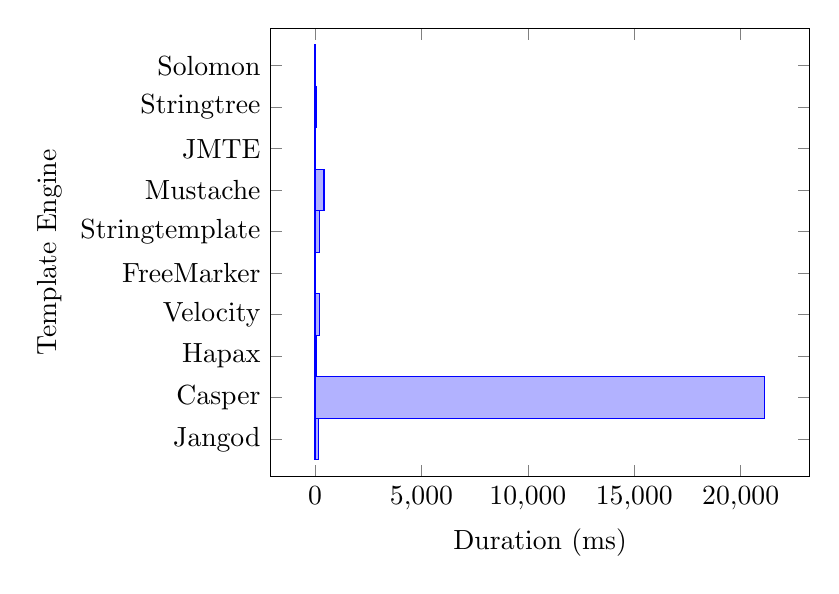
\begin{tikzpicture}
\begin{axis}[
    scaled ticks=false,
    % xmode=log,
    % ticks with fixed point,
    % scaled ticks=false,
    xbar stacked,
	bar width=15pt,
	% nodes near coords,
    ytick=data,
    legend style={at={(0.5,-0.20)},
      anchor=north,legend columns=-1},
    ylabel={Template Engine},
    xlabel={Duration (ms)},
    symbolic y coords={
        Jangod, Casper, Hapax, Velocity, FreeMarker,
        Stringtemplate, Mustache, JMTE, Stringtree, Solomon
    },
    ]
\addplot+[xbar] plot coordinates {
  (180.5,Jangod) (21138.3,Casper) (73.6,Hapax) (196.6,Velocity) (29,FreeMarker)
  (196.6,Stringtemplate) (418.8,Mustache) (17.4,JMTE) (86.5,Stringtree) (8,Solomon)
};
\end{axis}
\end{tikzpicture}
\caption{Mean test duration by \gls{template engine}}
\label{fs:graph:duration}
\end{figure}


\begin{figure}[ht]
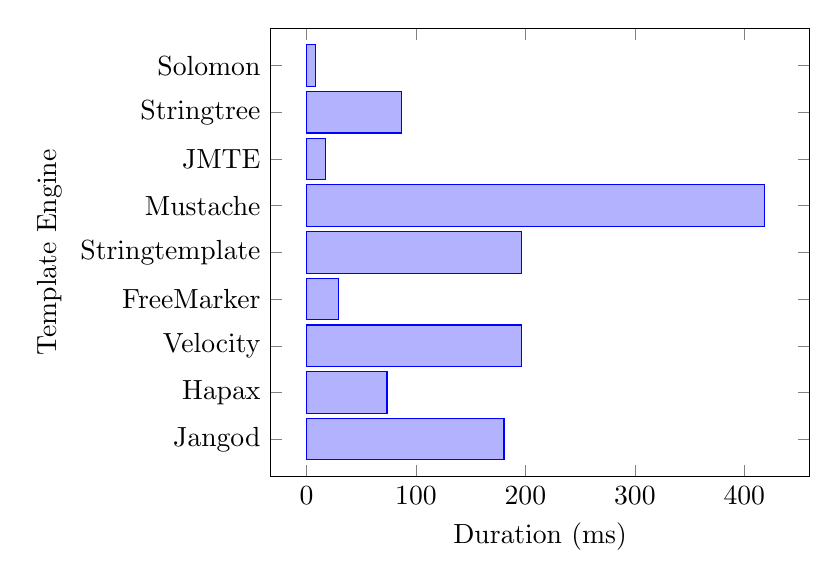
\begin{tikzpicture}
\begin{axis}[
    scaled ticks=false,
    % xmode=log,
    % ticks with fixed point,
    % scaled ticks=false,
    xbar stacked,
	bar width=15pt,
	% nodes near coords,
    ytick=data,
    legend style={at={(0.5,-0.20)},
      anchor=north,legend columns=-1},
    ylabel={Template Engine},
    xlabel={Duration (ms)},
    symbolic y coords={
        Jangod, Hapax, Velocity, FreeMarker,
        Stringtemplate, Mustache, JMTE, Stringtree, Solomon
    },
    ]
\addplot+[xbar] plot coordinates {
  (180.5,Jangod) (73.6,Hapax) (196.6,Velocity) (29,FreeMarker)
  (196.6,Stringtemplate) (418.8,Mustache) (17.4,JMTE) (86.5,Stringtree) (8,Solomon)
};
\end{axis}
\end{tikzpicture}
\caption{Mean test duration excluding \emph{Casper}}
\label{fs:graph:duration-excluding}
\end{figure}

It is reassuring that all the template systems in the study were capable of processing both plain text (S0) and simple substitution (S1) cases. However, these were the only scenarios that all the \gls{template engine}s passed. For all the other test scenarios there was at least one \gls{template engine} that could not manage it. There were only four \gls{template engine}s in the sample that correctly rendered every scenario: \emph{Solomon}, \emph{Stringtree}, \emph{Freemarker}, and \emph{Casper}. Given that these scenarios were chosen as representative of common situations in professional software development, it is surprising that there was so much variability in features. The documentation for all the implementations makes some kind of claim of being \enquote{powerful}, \enquote{flexible} or \enquote{suitable for a wide range of projects}. 

Consider, for example, the \emph{Hapax} template system that failed five of the eight tests. Its documentation states:

\begin{displayquote}
Hapax is a simple but powerful text templating library for Java. Hapax is suitable for constructing text output from Java code. The syntax is similar to Google's ctemplate library, and emphasizes the separation of logic from presentation. Hapax was designed to be easy to use and have minimal dependencies. Hapax does not depend on any existing web framework, and is suitable for use in servlets, scripting languages (Scala, Groovy, etc), and server-side applications.
\end{displayquote}

Nowhere in this does it mention any limitations, making comparing implementations on documentation alone a tricky proposition. Attempts have been made to compile comparative lists of such software by features \citep{Wikipedia2018} but interpretation of the exact meaning of each feature can be loose, and there would potentially be great benefit in defining a comprehensive set of such benchmark scenarios that could be used to compare and evaluate even software that is not found in such lists. The production of such benchmark scenarios would be difficult, however, because of the wide differences between \gls{template language}s. There is currently no single \enquote{meta language} in which scenarios can be expressed for multiple \gls{template engine}s. This problem is explored further in \autoref{chapter:intermediate}.

In many cases the limitations of the \gls{template engine}s seem closely tied to the choice of \gls{template language}. The minimalist language common to many \emph{Mustache} implementations, for example, deliberately avoids constructs such as loops, in favour of performing such logic in application code before invoking the \gls{template engine}. While this can be a workable strategy, and satisfies \citeauthor{Parr2004}'s (\citeyear{Parr2004}) desire for separation of concerns between view and model, it also has some potential drawbacks. Preparing values requires extra processing in the application code, which partially disguises the processing cost of generating pages compared to more competent \gls{template engine}s. It also requires that every possible configuration of data for the page is pre-calculated, including \enquote{expanding} collections. While expanding lists of textual or numeric values is relatively simple, this approach becomes much more complex in the relatively common case where each entry in the list needs to be processed using a secondary template in order to generate the desired result. This approach also denies the \gls{template engine} any possibility of automatically re-using intermediate values or using \enquote{lazy evaluation} strategies to avoid unused calculations, for example when Boolean conditions remove the need for a value to be rendered. Such choices have considerably more impact when the same application code is used to evaluate a wide variety of templates, each with different data requirements. In common with many software development habits, which prioritise development effort over execution time, it can be easier for developers to produce general-purpose code that pre-calculates everything required by every possible template, even though many of those values will not be required for any given rendered page. This can add extra, unneeded, processing cost to every page.

\label{A126}
There is also an anomaly in the timings. In table 3.2, it appears that several of the \gls{template engine}s take longer to process a plain text file than a simple substitution. While this is possible, it seems somewhat unlikely, so the experiment was temporarily adjusted to run the tests in a different order. Whichever test runs first seems to take longer. It was hypothesised that this was due either to interaction between the different template engines, or to some form of \enquote{warm up} behaviour. These issues cast doubt on the accuracy of the feasibility study model for performance comparisons, so an improved performance study was constructed to eliminate these kinds of influences. This improved performance study is described in \autoref{section:fs2}.

Despite these limitations, the feasibility study serves its purpose of determining whether the performance differences between different \gls{template engine}s were worth investigating further.

The software \enquote{test bench} for these measurements was constructed using the strategy pattern (as shown in \autoref{fs:figure:strategy}) with all the \gls{template engine} libraries loaded into memory at the same time. This made running the experiments much simpler, as they could be performed by a simple loop through a collection of \emph{TemplateSystem} objects with no need to stop or start the code, or to add and remove external code blocks. However, this approach also required some careful coding to deal with potential clashes and incompatibilities between the separate template libraries and their transitive dependencies. The version of Java used for these experiments did not provide any form of separation between libraries beyond class and package names. Any problems with any of the \gls{template engine} implementations (such as a syntax error in a template specification) that caused the \gls{template engine} to \enquote{crash} or raise an exception, would abort the whole test run. It is not clear whether there was any more subtle interference between the separate libraries that may have affected the results.

The approach of treating this code as a \enquote{throw away} experiment and writing only the minimum code necessary to perform the experiments had an impact on the usability of the software. Result values were simply printed out as soon as they were calculated, without performing any analysis or data formatting. This required manual copying into analysis software to determine derived results such as the mean duration. Configuration parameters such as the collection of \gls{template engine}s to be tested and the number of times to invoke them were hard-coded into the software, which meant that any change required editing and re-compliation of the experiment code.

Finally, it is important to note that this feasibility study only measured two things: the ability to correctly render some specific scenarios, and the time taken to perform them. While some \emph{guesses} may be made about what that might mean for overall energy usage, this study does not say anything definitive about the energy usage of the different \gls{template engine}s.

Later sections in this chapter and later chapters in this thesis address these issues. Improvements to the construction and operation of the test framework and more detailed  comparison of component performance are discussed in \autoref{section:fs2}. An apparatus for comparing the energy usage of software is developed in \autoref{chapter:testrig} and the energy usage of template engines is explored in \autoref{chapter:comp energy}.

\subsection{Analysis of Individual Template Engines}
\label{sub:individual template engines}

\emph{Casper} takes so long to perform the experiments that it makes \autoref{fs:graph:duration} unusable for comparing the performance of the other \gls{template engine}s. By removing Casper from the results (see \autoref{fs:graph:duration-excluding}) a more nuanced view of their relative performance can be seen.

In \autoref{fs:graph:duration-excluding}, \gls{template engine} performance can be seen to cluster into a few groups. \emph{Mustache} is in a group of its own, with a mean duration of 418.8ms, taking roughly twice the time as the engines in the next group. The next group contains three \gls{template engine}s: \emph{Stringtemplate}, \emph{Velocity}, and \emph{Jangod} all of which take around 200ms A third group includes \emph{Hapax} and \emph{Stringtree}, which both take a bit less than 100ms to complete the run. The final, fastest, group includes \emph{Solomon}, \emph{JMTE}, and \emph{Freemarker}, all taking 30ms or less.

It is clear from these results that the performance of different \gls{template engine}s varies widely. Examining the code and templates of the different template engines shows some interesting characteristics.

\begin{itemize}

\item \emph{Casper} has obviously been designed to be as flexible as possible, going so far as to start a complete JavaScript interpreter for every page generated, and discarding it when the page is completed. This imposes a relatively huge burden on generating regular web pages but does potentially provide some facilities unavailable in most other systems. It is important to note that this feasibility study was designed based on common web page scenarios, and thus does not include any cases where Casper would be the only applicable solution.

\item \emph{Solomon}, on the other hand has been coded with an emphasis on speed. It uses a relatively non-standard \gls{template language} (see \autoref{section:comp:languages}), optimised for simple and fast processing rather than easy readability and the internal design minimises time consuming operations such as parser-backtracking, buffering and data copying.

\item \emph{Stringtree} uses a similar \gls{template language} to Solomon but did not achieve the same performance benefits. When Stringtree was coded, performance was not the primary goal.

\item Two other template engines (\emph{JMTE} and \emph{FreeMarker}) achieve speeds almost as fast as \emph{Solomon}. \emph{FreeMarker} was also one of the few template engines that also managed to produce correct output for all the scenarios, which indicates that it is capable as well as fast. \emph{JMTE} and \emph{FreeMarker} have apparently also been coded with speed in mind, although their \gls{template language}s are more complex to parse than the language used by \emph{Solomon}, which may contribute to their slower performance. 

\item Simplicity of a \gls{template language} is no guarantee of performance, however. \emph{Mustache} has one of the simpler \gls{template language}s but performed the worst of the non-\emph{Casper} template engines. \emph{Hapax} and \emph{Jangod} have \gls{template language}s that are similar in many ways to \emph{Mustache}, but exhibit different performance characteristics. 

\item The remaining two templates in this study (\emph{Stringtemplate} and \emph{Velocity}) show similar performance to each other even though they have different \gls{template language}s and design goals.

\end{itemize}

The difference in template processing speed between the template engines in this study indicates that even when the platform and the task (generating specific output text) are fixed, choices during the design of \gls{template language}s and template engine implementations can significantly affect performance. 

\label{A135}
If the above experiments were used to select a \gls{template engine} for a project based on performance, then the three \gls{template engine}s in the fastest group would form the short-list. Selecting between these three would then depend on further factors. \emph{Solomon} is clearly the fastest. It is also able to correctly perform all the scenarios, so is the obvious choice. However, Solomon uses a slightly unusual \gls{template language} (see \autoref{section:comp:languages}) and this could require training that might hinder adoption. JMTE is the second fastest, but could not correctly perform all the scenarios. In development situations where the missing features are not important, however, then JMTE could be a good compromise. \emph{Freemarker}, although it is up to 18 times slower than Solomon for some cases, was the only popular \gls{template engine} to correctly perform all the scenarios. \emph{FreeMarker} also has the advantage of a well-documented \gls{template language} and wider adoption than the other two, so would also make a good choice for a more conservative development team. Based on their performance it would seem a poor choice to select any of the others.

\section{Feasibility Study Discussion}
\label{fs:discussion}

A key finding to arise from the feasibility study is the surprising variety in capabilities and performance between purportedly similar software libraries. The largest range in performance for a single scenario was for the Boolean False scenario between \emph{Casper}, which took 21572ms to complete the 10,000 template expansions, and \emph{Solomon}, which took 2ms. This is a difference of 10786 times. An application using \emph{Solomon} for this scenario would be able to process over 10,000 documents in the time it takes \emph{Casper} to process one. To handle a similar load, the machine running \emph{Casper} would need to be over 10,000 times as powerful. If that was not possible, multiple machines would be needed.

Even averaged across the range of different scenarios, the mean time taken for \emph{Casper} to perform the suite of scenarios (21138.3ms) is still over 2,500 times more than the mean time taken by \emph{Solomon} (8ms).

Selecting a \gls{template engine} for use in a software project is a difficult task. Typical open source software documentation has no quantitative specifications. All the components evaluated in this study are free software, so the traditional approach of minimising the purchase cost does not apply. All the components are available with licences that permit inclusion in commercial software, so considering licence terms is also no use in selecting between them. Despite their free availability, and with no direct financial incentive to increase \enquote{sales}, they often provide documentation that reads like optimistic and unsubstantiated advertising copy. Such documentation as is provided tends to concentrate on listing and describing specific available features, covering everything else with blanket subjective statements such as \enquote{fast}, \enquote{powerful} or \enquote{flexible}. This paucity of information makes it hard for developers to make informed choices.

The fact that one \gls{template engine}, \emph{Solomon}, was able to correctly perform all the scenarios in a much faster time than any of the others when they are all written in the same \gls{programming language} and running on the same platform, shows that the choices made in the design and programming of the different \gls{template engine}s in this study have had a huge impact on the performance and capabilities of these supposedly equivalent components. In this specific case, one reason could be that \emph{Solomon} was written to minimise multiple handling of template characters. Whenever possible, input characters are passed directly to the output document without buffering. The characteristics of the \emph{Solomon} \gls{template language} (discussed in more detail in \autoref{section:comp:languages}) help reduce the need for buffering.

\label{A139}
In conclusion, the results of this feasibility study show that there are surprisingly large differences in capabilities and performance between superficially similar solutions to a specific class of problem. The study provides data unavailable from the on-line documentation for the components being considered. This in turn suggests that a change in software development behaviour, both when writing software and when selecting components or libraries, could potentially make a noticeable difference in performance, and by implication the processing requirements and resource usage of large software systems such as the world wide web.

In particular, the following specific conclusions will be taken forward from this feasibility study:

\begin{itemize}
\item The differences between this sample of components are large enough to be worth proceeding with the research.
\item Choices made during design and development of software, and when selecting components, can have a large impact on the performance of the final product.
\item The methodology of constructing a range of representative scenarios and using them to compare the different components is fundamentally sound, however, improvements are needed to the implementation of the tests
\item The \gls{template language}s used by the different \gls{template engine}s vary widely enough that further research is needed on ways to simplify the creation of equivalent templates for a range of \gls{template engine}s.
\item Further research is needed to determine what impact this wide variety in performance might have on energy usage.
\end{itemize}

\section{An Improved Performance Study}
\label{section:fs2}

The following sections address the shortcomings of the feasibility study to enable a deeper exploration of the performance characteristics of \gls{template engine} components.  The development of an improved framework for the evaluation of components, and the results from using it for a wider range of performance comparisons is discussed in \autoref{section:comp:framework}.

\subsection{Recap of Problems With The Feasibility Study}
\label{section:comp:recap}

The feasibility study was conducted to gain an overview of the scale of the differences between a selection of components. While the results were clear, the individual performance measurements were neither rigorous nor comprehensive. In particular, the following issues were discovered:

\begin{itemize}
    \item \textbf{Problem 1} All the \gls{template engine}s were loaded into memory at the same time, which could cause influence between different components.
    \item \textbf{Problem 2} Clashes, both between class and package names of components and where components required different versions of the same library.
    \item \textbf{Problem 3} Configurations were all hard-coded, requiring editing and re-compilation of the code   \item \textbf{Problem 4} An anomaly in the timings where whichever scenario was run first took extra time.
    \item \textbf{Problem 5} Scenarios were always run the same number of times, and therefore showing only how the components compare at that load.
    \item \textbf{Problem 6} Results output was simplistic and difficult to process.
\end{itemize}

\subsection{Changes to the Component Landscape}
\label{section:comp:changes}

All of the \gls{template engine} components evaluated as part of the feasibility study were open source and free of charge and were chosen to be broadly representative of the available software at the time. However, in the several-year period between the feasibility study and the later measurements of the components (see the research timeline in \autoref{section:timeline}), the landscape of software in this niche had changed and developed. This is a natural process in open source software \citep{Sonatype2023} \citep{Xie2009}. While the \gls{template engine}s evaluated in the feasibility study were all still available, many had not been updated or were no longer in popular use. Several other \gls{template engine}s had appeared or increased in popularity in the intervening time. Research was needed to determine an appropriate set of current \gls{template engine}s to evaluate in more detail.

\subsection{Selecting Template Engines to Compare}
\label{section:comp:selecting}

For this stage of the research a more systematic approach was needed. This comprised the following initial steps to build a list of candidate \gls{template engine}s:

\begin{enumerate}
    \itemsep -0.5\parsep
    \item Limit the search to the \emph{GitHub}\footnote{\url{https://github.com/}} code repository
    \item Perform a search for the term \enquote{\gls{template engine}}.
    \item Limit the results to code in the Java language.
    \item Ignore repositories that are not textual \gls{template engine}s in their own right such as adaptors, plugins, examples, game engine templates etc.
    \item Ignore special-purpose \gls{template engine}s with specific output formats such as PDF, DOCX, and SQL.
    \item Ignore \gls{template engine}s that are obviously based on the \enquote{Template Engine Kata} from \citet{Koskela2007}.
    \item Ignore \gls{template engine}s that are \enquote{forks} of other \gls{template engine}s in the list
    \item Ignore \gls{template engine}s with documentation in languages other than English.
\end{enumerate}

This process resulted in a list of 132 \gls{template engine}s. The full list with names and GitHub URLs can be found in \appref{appendix:engines}. Note that, as mentioned above, the open source software landscape is continually changing, so following the same process at a later date would produce a different, and probably larger, set of results.

Even having eliminated the obvious cases where \gls{template engine}s appeared to have been created purely as a learning aid, there were still many in the list that were either incomplete, unusable, or would be unlikely to be used by anyone other than the original developer. To get perspective on which \gls{template engine}s to consider further, some gauge of popularity was needed.

Unfortunately, there is no single resource that indicates the popularity of such software components. Commercial products do not usually reveal their choice of components. Some code repositories provide indications of the number of times a particular component has been downloaded, or how many times it is used by other projects in the same repository. While such statistics can give clues as to the popularity of components, they are not reliable. For example, download counts are easily skewed if some organisation has a policy of re-downloading every component for every build, which may happen many times per day. Statistics on the usage of components by other components are arguably more useful, but are limited to dependencies that the repository is aware of, and do not include code that is not stored in a public component repository.

On the wider internet, there are a range of personal and collaborative websites containing recommendations and comparisons. These websites can provide an indication of popularity. Individually, each such website is of limited use. The information provided may not be objective and has probably never been reviewed. The site may be out of date, presenting information on obsolete versions of components. The authors may have misunderstood the capabilities of individual components, or be unaware of the existence of some, or lack the skills or experience to fully evaluate the options. In some cases the information may be deliberately or accidentally biased.

When a range of such resources are considered as a whole, however, they can provide a kind of \emph{zeitgeist}, but there are still potential problems. While outright collusion is less likely when a broad enough group of websites is included, there is still the possibility of an \enquote{echo chamber} effect \citep{Cinelli2021}, in which the creator of each website gains their information mainly from other similar websites. Such effects tend to reinforce the popularity of well-known choices and exclude newer or less-familiar opinions. The main reason to include this source of information in this research is because it is the main public source of information available to software developers. Individual developers will often have other sources, such as personal experience, the opinions of colleagues or friends, or instructions from an employer or client, but such sources are largely private and were unavailable for this research.

Public information sources on the web can be grouped into categories, with the elements in each category having different characteristics.

\paragraph{Data from component repositories} As discussed above, the details provided by component repositories vary and may not be fully representative, but within their scope they are authoritative.
    
\paragraph{Open Forums and Discussion sites} These kinds of sources typically consist of questions and answers, although there are often multiple answers to a question and the responses may conflict with each other or digress from the original topic. Typical examples include sites aimed at software developers such as \emph{Stack Overflow}\footnote{\url{https://stackoverflow.com/}} and \emph{The Java Ranch}\footnote{\url{https://javaranch.com/}} as well as more general question-and-answer sites such as \emph{Quora}\footnote{\url{https://www.quora.com/}} and \emph{reddit}\footnote{\url{https://www.reddit.com/}}. Some such sites have mechanisms intended to emphasise credible answers, or at least credible participants. Others make no such judgement.
    
\paragraph{Crowd-sourced Comparisons} In crowd-sourced websites, multiple users contribute to collecting and organising information and provide some notion of consensus. The most well-known website of this nature is \emph{Wikipedia}\footnote{\url{https://www.wikipedia.org/}} but this category also includes other \enquote{wiki} style websites as well as review aggregators such as \emph{Capterra}\footnote{\url{https://www.capterra.com/}}.
    
\paragraph{Individual Opinions} This category includes websites, blogs, videos, podcasts, articles, and social media posts predominantly created and managed by a single individual. The form of these opinions varies widely as does the scope. This category also includes articles or chapters in non peer-reviewed publications or collaborative websites, as long as there is an identifiable author. The key point with the sources in this category is that they originate from one individual and reflect that person's opinions, or at least what they would like to present as their opinions. In some cases there may be opportunities to engage with the author through comments or direct messages, which can help to justify or clarify their opinions.
    
\paragraph{Provider opinions} The final category includes all information in which the creator, provider or vendor of a particular product has a stake of some sort. The most common example of this is documentation websites provided for users of their product or products, but this category also includes forums, discussion sites, and blogs owned or managed by a stakeholder in a particular product. Such sources are usually the most authoritative in regard to their own products, but have an inherent bias and cannot be relied on for information about competing products.

This research included sources from each of the above categories. A full list of sources consulted is given in \appref{appendix:sources}. In addition to the \gls{template engine}s in the original feasibility study, several potential new candidates were identified. Not all were technically suitable to be included in the comparison, but this was not discovered until an attempt was made to include them in the experiments. Details are given in \autoref{section:comp:testing}.

\section{A Framework for Interchangeable Components}
\label{section:comp:framework}

The testing and evaluation of software components requires a different approach to the normal process of component-based software development. When developing a software product that uses third-party components, the main aim is usually to integrate those components closely with the rest of the code, to form a single application code base. When evaluating a range of components, on the other hand, the aim is to keep them as separate as possible from each other to minimise unintended influence on the evaluation. The feasibility study described in \autoref{section:fs1} was developed using a traditional integration approach and raised several issues that needed to be addressed in order to reliably measure and compare the components.

\subsection{Extracting Template Engines into Separate \enquote{Plugins}}
\label{section:comp:plugins}

To ensure complete separation between the different \gls{template engine} implementations, it was decided to re-code the measurement framework to treat the \gls{template engine}s as \enquote{plugins} to be loaded into the framework at run-time and tested individually. The Java language provides support for dynamic swapping of code, subject to the following constraints:

\begin{itemize}
    \item The code to be loaded must be in the form of compiled Java class files.
    \item The classes must have been compiled with a compatible version of the Java compiler.
    \item The plugins must all implement the same java interface.
    \item The classes to be loaded must be visible on the Java \gls{classpath}.
\end{itemize}

\label{A143}
All the selected template engines were written in Java and the source code was available. The availability of source code meant that they could be compiled to Java class files using the same version of the Java compiler as the test framework. This addressed the first two restrictions.

Even though all the \gls{template engine}s under consideration were written in Java, they all had different code with no interfaces or class names in common. This meant that they could not be called in the same way by the same code. To resolve this restriction, a \enquote{driver} was created for each \gls{template engine}. Each driver presents the same interface to the comparison framework but understands how to setup and invoke a particular \gls{template engine}.

The cohort of \gls{template engine}s considered for this study all use one of two ways of initiating the code for the \gls{template engine}. The traditional approach in Java is to use the Java \verb!new! operator to create an object of a named class. An alternative approach is to directly call a \verb!static! method on a named class that itself creates an appropriate object. In each case, the result is an object with methods that may be called for typical \gls{template engine} operations such as setting context values or expanding a template. The specific details of the methods available vary between \gls{template engine} implementations, with some requiring further setup and configuration while others are immediately ready to be used to process documents. Similarly, the specific sequence of methods and parameters to use when creating a context and expanding a template to produce a destination document also varies between \gls{template engine}s.

To ensure that the API for each engine was called in the correct manner, each plugin driver implements a Java \verb!interface! with two core methods: \verb!init()! to perform whatever initiation and preparation is required by the \gls{template engine} before it can be used; and \verb!expand()! that can be used to combine a named template with a provided context to produce an output document. 

Further details of the plugin driver implementation are given in \cref{appendix:driver}.

\subsection{Dynamic Loading of Plugins}
\label{comp:plugins:dynamic}

In order to compare the behaviour of each \gls{template engine} without overhead or interference from other \gls{template engine} code or data, it is vital that each \gls{template engine} driver is loaded independently. It is also highly desirable to be able to include new \gls{template engine}s without requiring changes to the code of the comparison framework. In order to meet this requirement, the code for \gls{template engine} drivers must be separate software, with the template comparison framework treated as a \enquote{black box}. In this approach, knowledge should be strictly one-way. It is acceptable for drivers to make use of classes from the framework code, such as the \verb!TemplateEngine! interface that all drivers must implement. However, it is not acceptable for the comparison framework to require knowledge of any classes from individual drivers as this would require those drivers to be present whenever the comparison framework is compiled.

The aim is that a \gls{template engine} evaluation can be run with a \gls{template engine} plugin specified as a command-line parameter. The comparison framework will then prepare and evaluate each comparison scenario and generate an appropriate destination document using the driver specified in the plugin. Unfortunately, in Java this process is not quite as simple as that would seem. In order to call methods on a driver, the driver must be instantiated as a Java object, which in turn requires that the class which specifies that object must be loaded first.

The Java language and virtual machine supports dynamic loading of classes, but with a catch. In Java there are essentially two ways to load a class. By far the most common is to refer to it by its fully-qualified name in the calling code. This approach, however, requires that the calling code know the full details of the package and name of the class to be loaded, which would violate the one-way knowledge rule, above. The alternative way to load a class involves techniques known as \enquote{reflection} and \enquote{introspection} that allow Java code to examine and use compiled Java objects without needing to know about their classes in advance. Reflection and introspection are relatively cumbersome to use, are known to be slower in use, and have a much wider range of failure modes than the regular way of using classes and objects.

There is, however, a way to gain the benefits of invoking a named class without knowledge of the details of the plugin. This requires the creation of a single class in every plugin that has the same fully-qualified name, in this case \verb!plugin.EngineFactory!. When the comparison framework code is compiled, it is provided with a \enquote{dummy} implementation of this class to avoid compiler errors about a missing class. When the comparison framework is run to evaluate a particular \gls{template engine}, the dummy class is removed from the \gls{classpath}, and the identically-named class from the supplied plugin is used instead. The intention is that this impostor class is as minimal as possible, leaving all the real work to appropriately-named classes within the plugin. 

Further details of the plugin driver factory implementation are given in \appref{appendix:driverfactory}.

The key method in this class is \verb!create!, which is responsible for creating a template-engine-specific driver object that implements the \verb!TemplateEngine! interface. Once that object is created, it can then be used by the template comparison framework, which only knows about the methods provided by the \verb!TemplateEngine! interface. The other method is not strictly necessary to generate templates, but aids observability of the comparison process and can be used in logging and error messages to indicate which plugin was in use when something happened. Note that as the shared interface has the same \enquote{leaf} name as the class being defined, it needs to be specified as a full-qualified name \verb!shared.EngineFactory! to avoid conflicts during compilation.

The \verb!create! method requires one parameter, a \verb!File! object representing a folder containing stored templates. Most of the \gls{template engine}s in this cohort require their templates to be stored on a file system, sometimes with specific requirements for file structure and naming. Arguably, \gls{template engine}s would probably perform faster and use less energy if template storage was in memory, without the overhead of locating and loading a template from slower file storage. However, while some of the \gls{template engine}s under consideration do support other forms of template storage, the only template source supported by all the \gls{template engine}s is templates stored on a file system, so for a more equable comparison of \gls{template engine} performance, all comparisons were done with templates stored in files.

While this approach of defining an identically-named class in every plugin addresses the problem of using plugin code without foreknowledge of the details of the plugin, it can cause some issues during development. Some Java development tools and integrated development environments (IDEs) prefer to load all the code for a project at once in order to build a search index and check for potential conflicts. Such tools do not work well with this style of coding. Happily, the Eclipse IDE\footnote{\url{https://www.eclipse.org/ide/}} used for the development of this code allows development in a \enquote{workspace} that consists of several separate \enquote{projects}, each of which contains its own independent namespace. Using Eclipse, the comparison framework and all the plugins could be worked on at once without the need to open, close, or switch projects.

The same approach to plugin loading and development was also used for the dynamic loading of \gls{template language} drivers that define the characteristics of different \gls{template language}s for use when generating test templates from an intermediate template (see \autoref{chapter:intermediate}).

\subsection{Conformance Testing of Individual Plugins}
\label{section:comp:testing}

Each plugin was developed and tested individually for conformance to the plugin specification described in \autoref{section:comp:plugins}. A conformance test framework was created using the \emph{JUnit}\footnote{\url{https://junit.org/junit5/}} testing tool to load and exercise each method of a specified plugin to ensure that it operated correctly. Example code to test a \gls{template engine} plugin is given in \appref{appendix:smoketest}. As will be seen later, the \gls{template language}s used by the various \gls{template engine}s varied considerably, so the tests could not be identical but each one had to be adjusted to use the correct \gls{template language} for the plugin being tested. A potential solution to this problem is discussed in \autoref{chapter:intermediate}.

\section{Replicating the Original Tests Using the New Plugins}
\label{section:comp:test replication}

Once a selection of plugins supporting a range of \gls{template engine}s had been created and tested, the next step was to replicate the feasibility study experiments using the new framework, to see how the results compared with the original. This involved re-working the original code to use the plugin API described above rather than the custom code that had been written for the different \gls{template engine}s in the original study.

\subsection{The Test Runner}
\label{section:comp:test runner}

One of the key aims for the reworking of the \gls{template engine} comparisons was to ensure complete isolation between the different \gls{template engine}s. The original performance comparison described in \autoref{section:fs1} had loaded the code for all the \gls{template engine}s into a single application and run a complete suite of tests for all loaded \gls{template engine}s in a single run of the code. The redesigned comparison framework not only separated out the \gls{template engine} code into dynamically loadable plugins but also separated the evaluation of individual scenarios into separate test runs. This was to make sure that there were no lingering side-effects from one scenario affecting the next. For compatibility with the original set of measurements, the same selection of scenarios were used. The new test runner is illustrated with a UML sequence diagram [\autoref{comp:figure:sequence}], which may be contrasted with the similar diagram from the feasibility study [\autoref{fs:figure:sequence}].

\begin{figure}[ht!]
\centering
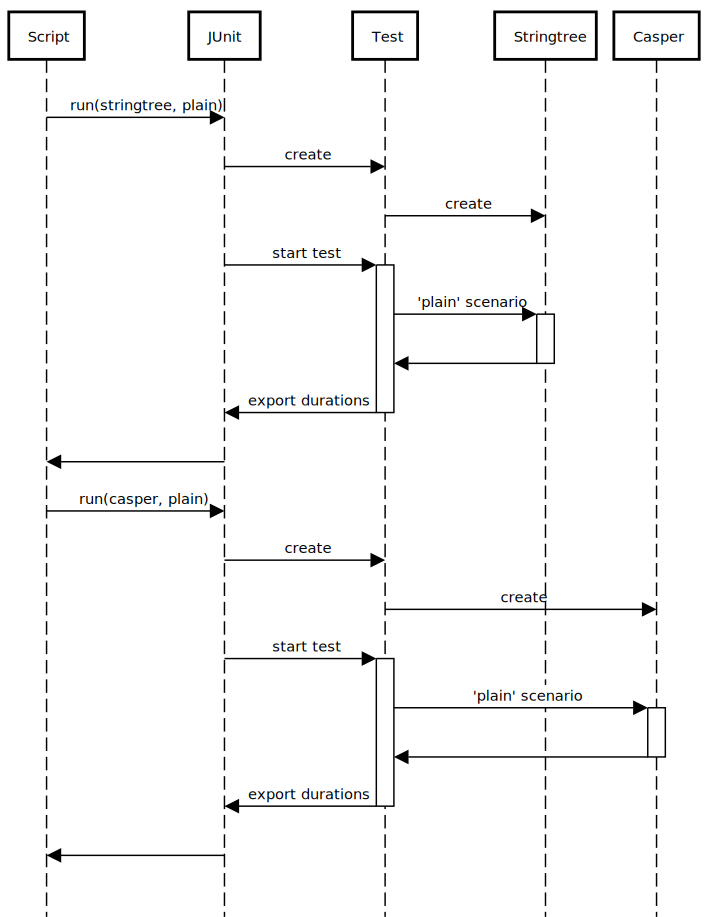
\includegraphics[scale=0.5]{Figures/newsequence.png}
\caption{Sequence diagram for the improved performance test process}
\label{comp:figure:sequence}
\end{figure}


When analysing the results of the original feasibility study it became clear that the experimental design was limited in several aspects. The plugin model enabled a way to evaluate individual \gls{template engine}s without interference from any of the others. The original experiments were also hard-coded to a specific number of expansions of each template. While implementing and testing the plugins it appeared that \gls{template engine}s have different performance characteristics as well as different rendering speeds for individual templates. To determine how these characteristics affect overall performance, a further series of experiments were designed that would measure the time taken to render different quantities of each template.

The test runner main routine reads command-line parameters to obtain the parameters for the test run, then loads and initialises the specified \gls{template engine}, loads the details of a specific scenario and the expected outcome, populates a context with the specified values, and then calls the \gls{template engine} to expand the provided template the specified number of times. Results were collected for each triplet of (\gls{template engine}, scenario, number of expansions) and are analysed in \autoref{fs2:results}.

An extra command-line option is also supported.\verb!-v! (for \enquote{verbose}) enables extra diagnostic messaging for use when tracking down problems when evaluating a \gls{template engine}. The verbose option was only used while setting up the comparisons. All timed runs had \enquote{verbose} disabled.

In Java, the entry point to an application is a \verb!main! method, and the \verb!main! method for the \verb!Run! class, which executes a particular test scenario is shown in \appref{appendix:testrunner}.

Each test scenario is stored in a folder and consists of two files. One file is the output document that is expected to be produced when the scenario is run. The contents of this file will be checked against the output that is actually produced by each \gls{template engine}. The other file is a \enquote{properties} file\footnote{\url{https://docs.oracle.com/cd/E23095_01/Platform.93/ATGProgGuide/html/s0204propertiesfileformat01.html}} that contains the specification of the scenario. A properties file consists of a set of key/value pairs. Each pair is positioned on a separate line of the file and takes the form \emph{key}=\emph{value} or \emph{key}: \emph{value}. The properties file used to specify a test scenario has one mandatory entry with the key \verb!~template!. The value associated with this key is the name of the template to be expanded. When the scenario is run, this template name will be used to locate the template within a folder of templates specific to the \gls{template engine} being evaluated. The properties file does not require other entries, but any other entries in the properties file will be used to populate the template context before expanding the template.

In a basic properties file, all keys and values are text strings. For some of the scenarios, however, the template context needs to be populated with values that are not simple strings. To enable this, all the context values in the properties files are processed using a filter that detects and converts values to different types. Each property key is examined for the presence of certain indicator characters at the end. If no indicator characters are present, then the key is used as it is and the value is treated as a text string. The presence of any of the indicator characters causes the value to be converted to the associated type. After conversion any indicator characters are removed from the key before adding the value to the template context. As an example, the properties file in \appref{code:properties example} will result in the use of a template named \enquote{cond} with a template context containing a single entry named \enquote{yes} with a value of boolean \emph{false}.

\begin{lstlisting}[backgroundcolor=\color{black!5},backgroundcolor=\color{black!5},escapeinside={(*}{*)},tabsize=2,label={code:properties example},caption={Example `properties' file},captionpos=b]
~template: cond
yes?: false
\end{lstlisting}

The initial set of indicator characters are listed in \appref{table:indicator characters}

\begin{table}[ht!]
\centering
\begin{tabular}{lcc}
\textbf{Character} & \textbf{Resulting Type}  & \textbf{Value} \\
\hline
\verb!?!   & \verb!java.lang.Boolean! & \emph{true} if it starts with \verb!T! or \verb!t! \\
\verb|!|   & a new object of a specified type & fully qualified class name \\
\verb![!   & \verb!java.lang.Array! & comma-separated list of strings \\
\verb!>!   & a reference to another value & the key of the other value \\
\end{tabular}
\caption{Indicator characters for key/value conversion\label{table:indicator characters}}
\end{table}


\subsection{Experimental Process}
\label{comp:experimental process}

The aim of this experiment was to address the problems with the original study, as described in \autoref{section:comp:recap}. Problems 1 (all \gls{template engine}s in memory at one time) and 2 (class and package name clashes) were addressed by the introduction of the \gls{template engine} driver model and the dynamic loading of a single driver for each test run. Problem 3 (hard-coded configurations) was addressed by the use of enhanced properties files for scenario specification. Problem 4 (A timing anomaly with the test order) is no longer relevant, because in the re-coded architecture each test is run in isolation.

Problems 5 (the use of a fixed number of template expansions) and 6 (non-machine-readable results output) remained to be addressed by the design of the experimental process.

To address problem 5, the number of template expansions was added as a run-time parameter to an experiment run. This allowed test runs to be controlled by a script that could measure the time to run a specific scenario using a specific \gls{template engine} for a range of different quantities of expansions. Each scenario for each \gls{template engine} was initially tested by hand with a small range of quantities to ensure that the test runs and the time measurement worked correctly and produced repeatable results. Once all the scenarios for each \gls{template engine} were considered fit for further experiments, a script was developed to run each combination for a broader range of repetitions.

To address problem 6, the output data format was changed. The changes are discussed in \autoref{fs2:data}.

To enable evaluation of the performance of everything from a single expansion of a single scenario using a single \gls{template engine} to a full set of tests for every scenario for every \gls{template engine} at a range of numbers of repetitions, a series of scripts were developed. The more complex and long-running scripts were built to use the more specific and quicker tests. This also ensured that there was no accidental differences in the way experiments were performed between single specific runs and a full set. Where possible, scripts were coded to accept optional arguments, but apply reasonable default values if the arguments are not supplied.

The basic script, named \texttt{run.sh} is responsible for running a single scenario using a single \gls{template engine} a specified number of times. All the arguments are optional, but the \gls{template engine} name and the scenario name will usually need to be supplied in practice. If not supplied, the \gls{template engine} defaults to the \enquote{dummy} \gls{template engine} used when compiling the experiment framework (see \autoref{section:comp:plugins}) and the scenario defaults to the \enquote{plain} scenario that contains only boilerplate text and no \gls{template language} features. Calling this script with these defaults can be used to ensure that the script is working correctly, but is of little use for performance measurement. If no value is supplied for the number of repetitions, then the specified scenario will be evaluated a single time. This default value was frequently used when investigating issues and potential solutions to \gls{template engine} or \gls{template language} problems (see \autoref{comp:set 4}).

The Java language was not initially designed as a scripting languages that can be easily run from a command line. Java is a compiled language, which means that a compilation step is required before the code can be run. Java files are generally compiled using the \verb!javac! tool, although some development environments skip the tool in favour of calling the lower-level APIs used by that tool. The result of this compilation step is one or more \enquote{class files} (files whose names have a \verb!.class! suffix), which can then be executed by the Java Virtual Machine (JVM). Java class files are executed using the \verb!java! tool. When the result of the compilation step is a single class file that uses no external libraries or other components, executing it can be as simple as something like \verb!java HelloWorld.class!. However, Java projects that result in a single independent class file are relatively rare.

In the case of evaluating the performance of \gls{template engine}s, to execute a performance test requires access not only to the class files that comprise the comparison framework, but also to the class files that form the \gls{template engine} being evaluated. To include multiple class files when executing some compiled Java code, the JVM provides the notion of a \emph{\gls{classpath}}. A \gls{classpath} is formed from a list of class files, directories, and \enquote{jar} (java archive) files. When the code is executed, all the class files specified in the \gls{classpath}, and all the class files in the specified folders, and all the class files contained in the specified jar files are available for the code to use.

The \texttt{run.sh} script constructs a \gls{classpath} from the following:

\begin{itemize}
    \item The classes that comprise the specified \gls{template engine} driver, compiled into a directory named \enquote{bin} (for binary) in a directory named for the \gls{template engine}.
    \item The classes and libraries that comprise the specified \gls{template engine} itself, placed into a directory named \enquote{lib} (for libraries) in a directory named for the \gls{template engine}.
    \item The general-purpose classes used by the comparison framework and the \gls{template engine} drivers, placed into a directory named \enquote{shared/bin}
    \item The classes that comprise the comparison framework itself, placed into a directory named \enquote{bin}
\end{itemize}

Using the \gls{classpath} constructed as described above, the \texttt{run.sh} script calls the main method of the entry point of the comparison framework, the \verb!runner.Run! class. The name of the \gls{template engine}, the name of the scenario, and the number of repetitions, as well as any extra command-line arguments from the script are passed as arguments to the Java code, which then executes the evaluation. Additional command-line arguments are always optional but include, for example, a \verb!-v! (for \enquote{verbose}) option to enable extra diagnostic output during evaluations.

All the files and directories that are constructed into the \gls{classpath} are relative to the current working directory. For this script to function correctly, it must be started from the base directory of this project. If it is run from elsewhere, the required classes and data files will not be available, and the script will not be able to run.

The code for the \texttt{run.sh} script is given in \appref{appendix:run.sh}.

Building on the basic \texttt{run.sh} script, a second script, \texttt{one.sh} was developed to run the full suite of scenarios using a specified \gls{template engine}. In this script there is no scenario parameter needed, as it implicitly processes all scenarios. As with the \texttt{run.sh} script, the \gls{template engine} name is optional, defaulting to \enquote{dummy}, and the number of repetitions is optional, defaulting to 1. 

The list of scenarios to evaluate is not hard-coded in the script, but derived by listing the files in a \enquote{scenarios} directory relative to the current directory. This script scans the available scenarios, and calls the \texttt{run.sh} script with the name of each scenario as well as the specified \gls{template engine} name and number of repetitions. Just as with \texttt{run.sh}, this script must be run from the base directory of this project so that it can find all the files it needs.

The code for the \texttt{one.sh} script is given in \appref{appendix:one.sh}.

The next step beyond the \texttt{one.sh} script is a script (\texttt{all.sh}) that runs all the available scenarios for all the available \gls{template engine}s. As with the \texttt{one.sh} script, there is no need to specify the scenario name or the \gls{template engine} name, as this script scans directories to find both the list of scenarios and the list of \gls{template engine}s to evaluate. The number of repetitions is still optional and defaults to 1, as in the previous two scripts.

This script, while broadly similar in structure to the \texttt{one.sh} script, contains some extra processing to determine which directories contain a valid \gls{template engine} driver. The main technique used for this is to search each directory for a file named \texttt{EngineFactory.java}. This file is the entry point for a dynamically loaded \gls{template engine} driver, as discussed in \autoref{section:comp:plugins}. Any directory that does not contain this file cannot contain a \gls{template engine} driver. In addition to looking for the \gls{template engine} driver entry point, the \texttt{all.sh} script also applies a further rule. Any matching directory that also contains a file named \enquote{SKIP} denotes an inactive \gls{template engine} driver that should not be evaluated. This feature was initially implemented to exclude the \enquote{dummy} \gls{template engine} driver from the evaluation process, but was later found to be useful when comparing a reduced set of \gls{template engine}s for other purposes.

Once the list of valid and active \gls{template engine} driver directories has been collected, each one in turn is passed to the \texttt{one.sh} script to evaluate that engine in the full suite of scenarios for the specified number of repetitions.

The code for the \texttt{all.sh} script is given in \appref{appendix:all.sh}.

\section{Measurement Sets}
\label{fs2:sets}

The performance comparison of the cohort of \gls{template engine}s were performed as a series of measurement sets. Each measurement set provided a different view on the performance of the selected \gls{template engine}s. Feedback from each measurement set was used to suggest improvements or alternative approaches for further sets.

Each measurement set was performed by running a \texttt{fulldata} script. Each \texttt{fulldata} script made use of the \texttt{all.sh} script described in \autoref{comp:experimental process} with a different pattern of repetitions to collect a set of measurement data.

The measurement sets performed during this experimentation are as follows:

\paragraph{Set 1} examined the performance of a single template engine (\emph{Solomon}) at a range of loads in detail.

The Set 1 version of the \texttt{fulldata} script (\texttt{fulldata1.sh}) used a simple linear shell \enquote{for} loop to start with one repetition and increase one by one until the feasibility study maximum of 10,000. It became apparent that for some of the \gls{template engine}s this process would take a prohibitively long time, so this approach was abandoned.

The code for the Set 1 \texttt{fulldata1.sh} script is given in \appref{appendix:fulldata1.sh} and the results of Set 1 are explored in \autoref{comp:set 1}.

\paragraph{Set 2} reduced the level of detail in order to compare all of the selected template engines against all the scenarios at a range of loads.

To gain a quick insight into the major differences between the \gls{template engine}s, the Set 1 script was copied to \texttt{fulldata2.sh} and re-coded to instead perform a simple logarithmic experiment, executing each combination of scenario and \gls{template engine} 1, 10, 100, 1000, and 10000 times. While the logarithmic script was successful in providing an overview of the relative performance characteristics of the different \gls{template engine}s, the results contained obvious artefacts related to the large jumps in the number of repetitions, and the attempts to interpolate between them.

The code for the Set 2 \texttt{fulldata2.sh} script is given in \appref{appendix:fulldata2.sh} and the results of Set 2 are explored in \autoref{comp:set 2}.

\paragraph{Set 3} introduced the \emph{Handlebars} template engine and excluded \emph{Hapax}, which overshadowed the other results. Set 3 also introduced averaging of multiple runs to decrease the impact of \enquote{noise} on the measurements.

A further version of the \texttt{fulldata} script was then written to gain more information about the performance of the \gls{template engine}s between the logarithmic steps. This approach attempted to improve the performance of the linear approach by using two slopes. To provide detail in the low end of the performance graph, this script increased the number of repetitions in increments of 10, rather than 1 for tests up to 100 repetitions. After this, the number of repetitions was stepped in increments of 100 up to the maximum of 10,000 repetitions. This took a long time, particularly for the slowest of the \gls{template engine}s, but the resulting data contained much more detail than the logarithmic script.

The code for the Set 3 \texttt{fulldata3.sh} script is given in \appref{appendix:fulldata3.sh} and the results of Set 3 are explored in \autoref{comp:set 3}.

\paragraph{Set 4} re-introduced \emph{Hapax} after a change to the \emph{Hapax} driver to reduce internal warning messages and thereby improve performance. A problem was also rectified in some of the \emph{Handlebars} templates that had been causing slow behaviour in the \enquote{iter} scenario. The inability of the \emph{Stringtemplate} \gls{template engine} to correctly include other templates was also addressed with a driver change.

This final version of the test script brought the test repetitions into a hybrid approach combining aspects of both the linear script and the logarithmic script. This approach increased the number of repetitions in steps of 10 up to 100, then steps of 100 up to 1000, then steps of 1000 up to 10000. While not exhaustive, this script was considered to be a reasonable compromise of providing enough information to characterise \gls{template engine} performance behaviour in a time that allowed for multiple runs of each set for subsequent averaging.

The code for the Set 4 \texttt{fulldata4.sh} script is given in \appref{appendix:fulldata4.sh} and the results of Set 4 are explored in \autoref{comp:set 4}.


\subsection{Data Collection}
\label{fs2:data}

To address problem 6 from the original measurements, The Java test runner was coded so that each execution of the test runner application resulted in a single CSV row of data. To gain a bigger picture of the relative performance characteristics of the different \gls{template engine}s required multiple runs of the test runner, so the experimental scripts were coded to append the data from each of the multiple runs with different parameters into a single CSV output file for analysis. The CSV output included columns for the date and time of the test run, the \gls{template engine} name, the scenario name, the number of repetitions, the time taken (in milliseconds) and an indication of whether the result of expanding the template produced correct output (indicated by \textbf{OK}) or incorrect output (indicated by \textbf{NOTMATCHED}). An example section of the CSV data might look as shown in \autoref{code:csv example}.

\begin{lstlisting}[backgroundcolor=\color{black!5},escapeinside={(*}{*)},tabsize=2,label={code:csv example},caption={Example of CSV output},captionpos=b]
2022-06-30T11:57:32,stringtree,iter,10,24,NOTMATCHED
2022-06-30T11:57:32,stringtree,plain,10,18,OK
2022-06-30T11:57:33,stringtree,separate,10,26,OK
2022-06-30T11:57:33,stringtree,single,10,19,OK
2022-06-30T11:57:33,jte,bean,10,1090,OK
2022-06-30T11:57:34,jte,cond-false,10,1043,OK
2022-06-30T11:57:36,jte,cond-true,10,1038,OK
2022-06-30T11:57:37,jte,include,10,1090,OK
\end{lstlisting}


One advantage of this format is that the content of the generated CSV results files are independent of the order of the entries. Each row contains enough information to uniquely identify it and its contribution to the results. This became especially important during analysis when it was desired to look at the average of several runs through the complete test suite. In principle, merging the data could be done by simply concatenating the data from the output files into a new single file that could then be processed by the analysis and graphing software. In practice, each CSV file starts with a header line, so simply concatenating the files would result in several such header lines interspersed with the data. As the header lines contain textual descriptions of the columns in the CSV data, they do not contain valid test data and would prevent correct functioning of any analytic or graphing software. A short script was coded in Python to accept an arbitrary list of these CSV output files and correctly concatenate the data, keeping only a single header line at the start.

In several of the sets of testing, the \texttt{fulldata} script was run more than once in an attempt to detect the effects of events and forces outside the behaviour of the \gls{template engine}s being evaluated. The measurements were performed on a Linux virtual machine running on a Windows PC, so there were two levels of underlying system, either of which could spontaneously use system resources on tasks unrelated to the \gls{template engine} performance experiments. While, as can be seen in the results in \autoref{fs2:results}, the overall character of the performance of each \gls{template engine} remained broadly the same, there was evidence of such external factors.

In an attempt to mitigate the effects of external interfering factors on the measurements, an additional script was also coded in python to read the output from multiple \texttt{fulldata} runs and produce a new output file containing the arithmetical mean of the time taken for each set of similar measurements from the provided data. The results of this attempt at smoothing the data can also be seen in \autoref{fs2:results}.

It is important to note that while care was taken to minimise changes in external factors such as hardware and software versions and other applications and processes running on the test platform during multiple runs for the same set, this could not practically be maintained between sets. Each set of testing therefore represents a comparison between the performance characteristics of the cohort of \gls{template engine}s but not an absolute measurement. The aim was that the overall relative characteristics would be repeatable if performed on other hardware and software systems, while the individual measurements would probably be different.

\section{Results}
\label{fs2:results}

As discussed in \autoref{fs2:sets},  the results from the performance comparison of \gls{template engine}s are gathered into a series of measurement sets. Each measurement set provides a different view on the performance of the selected \gls{template engine}s. Feedback from each measurement set is used to suggest improvements or alternative approaches for further sets. The details of each measurement set are described in the sections below, and overall discussion and conclusions are explored in \autoref{comp:fs2:dicsussion} and \autoref{comp:conclusions}. Where appropriate, results are illustrated by both large and small scale graphs. The small scale graphs fit a full set of 8 scenarios on a single page and provide an overview for direct visual comparison between the different scenarios. The large scale graphs provide clearer indication of the performance of individual \gls{template engine}s in the context of a single scenario.

\subsection{Set 1}
\label{comp:set 1}

As mentioned in \autoref{comp:experimental process}, the first set of performance comparisons was intended to measure the performance of each \gls{template engine} running each scenario at every step of repetitions from 1 to 10,000. This initially seemed plausible, with some of the faster \gls{template engine}s being able to complete their tests in just a few hours on the available computing hardware. A run using a slightly modified \texttt{fulldata1.sh} script  (see \appref{appendix:fullsolomon.sh}) that called the \texttt{one.sh} script using only the \emph{Solomon} \gls{template engine}, one of the fastest from the original study, completed in 306 minutes (over 5 hours). However, some of the slower \gls{template engine}s took tens or even hundreds of times longer to process the test scenarios in the original study, and would therefore possibly require many days to complete.

Examination of the results of running the modified \texttt{fulldata1.sh} script (shown in \autoref{results:fullsolomon}) showed no evidence of unusual performance characteristics at specific numbers of repetitions. What was clear, however, was the presence of \enquote{noise} in the results. The working hypothesis was that this was due to other software and hardware factors outside the software being tested. To eliminate such \enquote{noise} would require one of two techniques:

\begin{itemize}
    \item Curve fitting or smoothing could assist in providing a cleaner curve for the data, but would not necessarily be representative, as it would include the \enquote{noise} in its calculations.
    \item Averaging multiple runs would potentially provide a better solution, because any variation in results which is present in only a single data set would contribute proportionally less to the final result.
\end{itemize}

Averaging multiple runs was chosen as the more appropriate technique, and was used for measurement sets 3 (\autoref{comp:set 3}) and 4 (\autoref{comp:set 4}).
 
\begin{figure}[!p]
\centering
\includesvg[width=\columnwidth]{Figures/graphs/svg/2023-12-18.csv.svg}
\caption{\label{results:fullsolomon}Performance comparison set 1 overview illustrating the results of testing at every increment and the impact of noise on the readings (\emph{Solomon} only)}
\end{figure}

The combination of the apparent lack of need for this degree of detail, and the need to perform multiple runs for averaging, led to this approach being abandoned in favour of taking larger steps to achieve more results faster in further sets.

\subsection{Set 2}
\label{comp:set 2}

The second set of measurements used a logarithmic progression of repetitions, measuring the time taken by each \gls{template engine} to process each scenario 1, 10, 100, 1000, and 10000 times. Each run of this script completed much more quickly than the version in Set 1, which enabled a full set of all scenarios for all active \gls{template engine}s. The initial results are shown in \autoref{multi:set2}.

\begin{figure}[!p]
\centering
\includesvg[width=\columnwidth]{Figures/graphs/svg/2022-06-30.csv.svg}
\caption{\label{multi:set2}Performance comparison set 2 overview illustrating the way that the time taken by \emph{Hapax} in certain scenarios overshadows all other readings when presented at the same scale}
\end{figure}

Although the graphs in \autoref{multi:set2} go some way to indicating the relative performance characteristics of the different \gls{template engine}s, they are not very useful. The time taken by all the other \gls{template engine}s is completely overshadowed by the much worse performance of the loop scenarios (\enquote{iter} and \enquote{separate}) when evaluated using the \emph{Hapax} \gls{template engine}.

\label{A148}
Considering the full cohort of template engines on a single graph can make it difficult to clearly see differences between individual template engines. The same results from \autoref{multi:set2}, but with the \emph{Hapax} \gls{template engine} omitted from the graphs, are shown in more detail in \autoref{multi:set2-plain} to \autoref{multi:set2-separate}.

The graphs in \autoref{multi:set2-plain} to \autoref{multi:set2-separate} illustrate much more clearly the range of differences between the various approaches used by the different \gls{template engine}s. On the whole, all the \gls{template engine}s show a progressively increasing duration as the number of repetitions is increased, but they differ in three key aspects: the minimum duration, the slope of the increase, and the variation between scenarios. The minimum duration is indicative of some kind of \enquote{setup cost} incurred by the \gls{template engine} before it is able to expand a template. This contributes a larger proportion at low numbers of repetitions, and can make a \gls{template engine} with a high minimum duration seem as much as a thousand times worse than other \gls{template engine}s for low-volume use. The slope of the increase is indicative of the additional time take to process each repetition of the same template. This factor is most important at high numbers of repetitions. A \gls{template engine} with a steep slope can soon require much more time to process the same templates as a \gls{template engine} with a high minimum duration but a shallow slope of increase. These factors are not typically constant for each \gls{template engine}, however, but vary depending on the content of each template being expanded. The graphs for the different scenarios show considerable differences in slope and to a lesser degree, minimum duration between scenarios.

\label{A149}
In the data from Set 2, \emph{JTE} has a high minimum duration of around 1000ms but a relatively shallow slope of increase. This implies that in many cases, potentially at very high volumes of template expansions, it will eventually take less time to process all the templates than other \gls{template engine}s. However, this is not always the case. There are some \gls{template engine}s, such as \emph{Trimou} and \emph{Solomon}, which have both a low minimum duration \emph{and} a shallow slope.

\label{A155}
The performance results for each scenario are discussed below in a series of figures and tables that highlight the differences in low-volume (single run) and higher-volume (10,000 run) performance between each of the template engines for that scenario.

\paragraph{\enquote{plain} (no placeholders, just boilerplate text)}
\label{A150}
The results of the \enquote{plain} scenario are shown in \autoref{multi:set2-plain} and \autoref{w2:results:plain}.

In the \enquote{plain} scenario, both these \gls{template engine}s have very low minimum duration and, even at 10,000 repetitions, have only increased by 41ms (\emph{Trimou}) and 37ms (\emph{Solomon}) whereas \emph{JTE} has increased by 231ms (see \autoref{w2:results:plain}). Extrapolating from these results, it seems unlikely that either of these two \gls{template engine}s would ever perform worse than \emph{JTE} in this scenario, regardless of the quantity of template expansions.

\begin{figure}[!p]
\centering
\includesvg[width=\columnwidth]{Figures/graphs/wave2/single/2022-06-30-without-hapax.csv.plain.svg}
\caption{\label{multi:set2-plain}Set 2 performance comparison for the \emph{plain} scenario, excluding \emph{Hapax}}
\end{figure}

\begin{table}[!p]
\centering
\begin{tabular}{lrr}
\textbf{Engine} & \textbf{Single Run} & \textbf{10000 Runs} \\
\hline
trimou & 2 & 43 \\
solomon & 13 & 50 \\
freemarker & 104 & 260 \\
stringtemplate & 144 & 564 \\
stringtree & 17 & 276 \\
jte & 1016 & 1247 \\
jangod & 25 & 512\\
velocity & 7 & 607\\
pebble & 28 & 114 \\
thymeleaf & 346 & 635 \\
mustachej & 12 & 606 \\
\end{tabular}
\caption{Set 2 durations (ms) for the \enquote{plain} scenario\label{w2:results:plain}}
\end{table}

In this study, the \enquote{plain} scenario largely serves to measure the underlying performance of the \gls{template engine} including \enquote{setup costs} and the time to process a document. Without the presence of any placeholders, it does not provide information about the performance characteristics of each \gls{template engine} when processing different placeholders and directives. The remaining scenarios are investigated below.

\paragraph{\enquote{single} (a single replacement placeholder)}
\label{A151}
The results of the \enquote{single} scenario are shown in \autoref{multi:set2-single} and \autoref{w2:results:single}.

The performance curves for each \gls{template engine} in this scenario are broadly similar to the ones for the \enquote{plain} scenario, although most \gls{template engine}s exhibit a steeper slope of increase, indicating that they are doing more work for each template expansion. The main exception to this is \emph{JTE}, which has an almost identical curve to the \enquote{plain} scenario.

\begin{figure}[!p]
\centering
\includesvg[width=\columnwidth]{Figures/graphs/wave2/single/2022-06-30-without-hapax.csv.single.svg}
\caption{\label{multi:set2-single}Set 2 performance comparison for the \emph{single} scenario, excluding \emph{Hapax}}
\end{figure}

\begin{table}[!p]
\centering
\begin{tabular}{lrr}
\textbf{Engine} & \textbf{Single Run} & \textbf{10000 Runs} \\
\hline
trimou & 3 & 76 \\
solomon & 13 & 66 \\
freemarker & 101 & 262 \\
stringtemplate & 162 & 922 \\
stringtree & 16 & 378 \\
jte & 1037 & 1288 \\
jangod & 27 & 535 \\
velocity & 14 & 849 \\
pebble & 277 & 406 \\
thymeleaf & 418 & 903 \\
mustachej & 13 & 605 \\
\end{tabular}
\caption{Set 2 durations (ms) for the \enquote{single} scenario\label{w2:results:single}}
\end{table}

\label{A152}
Although \emph{JTE} still took more time than any of the other \gls{template engine}s, even at 10,000 repetitions, some of the ones with steeper slopes (such as \emph{Stringtemplate}, \emph{Velocity}, and \emph{Thymeleaf}) were approaching the \emph{JTE} minimum duration.

\label{A153}
The performance profile for the \emph{Pebble} \gls{template engine} warranted further investigation. In this scenario, as well as in the \enquote{bean}, \enquote{iter} , and \enquote{separate} scenarios, the \emph{Pebble} \gls{template engine} exhibits a relatively large minimum duration compared to the \enquote{plain}, \enquote{include}, \enquote{cond-true} and \enquote{cond-false} scenarios. The code for \emph{Pebble}\footnote{\url{https://github.com/PebbleTemplates/pebble}} makes use of \gls{lazy evaluation}, a technique in which the calculation or processing of data values is deferred until needed. It is significant that the \enquote{single}, \enquote{bean}, \enquote{iter}, and \enquote{separate} scenarios all require context values to be rendered. It appears that the apparent speed of \emph{Pebble} in scenarios without value rendering is a benefit of the lazy evaluation process. In practice, templates that do not include rendered values are very rare, so the relative speed of \emph{Pebble} in real use is likely to be closer to the performance in the \enquote{single} scenario.

\paragraph{\enquote{include} (include a second template)}

The results of the \enquote{include} scenario are shown in \autoref{multi:set2-include} and \autoref{w2:results:include}.

This scenario followed the progression from the previous two. \emph{JTE} was still the worst performing \gls{template engine} over the range of 1 to 10,000 repetitions, but several of the other \gls{template engine}s (\emph{Stringtemplate}, \emph{Jangod}, \emph{velocity}) were in the same area by the end of the range. \emph{Trimou} and \emph{Solomon} remain the best performing \gls{template engine}s in this scenario, both once again showing a shallower slope than \emph{JTE}, so likely to remain a more performant choice regardless of template volume.

The poor performance of the \emph{Stringtemplate} and \emph{Jangod} \gls{template engine}s in this scenario may be partly explained by their lack of full support for this operation. It appears that the ability to include templates is not included in \emph{Jangod} by design, so a failure in this scenario is to be expected. The documentation for \emph{Stringtemplate} claims that template inclusion is possible, however, but at this point in the experimentation, template inclusion in \emph{Stringtemplate} was not working. Template inclusion in \emph{Stringtemplate} was addressed in Set 4 of the measurements (see \autoref{comp:set 4}).

\begin{figure}[!p]
\centering
\includesvg[width=\columnwidth]{Figures/graphs/wave2/single/2022-06-30-without-hapax.csv.include.svg}
\caption{\label{multi:set2-include}Set 2 performance comparison for the \emph{include} scenario, excluding \emph{Hapax}}
\end{figure}

\begin{table}[!p]
\centering
\begin{tabular}{lrr}
\textbf{Engine} & \textbf{Single Run} & \textbf{10000 Runs} \\
\hline
trimou & 2 & 55 \\
solomon & 12 & 67 \\
freemarker & 104 & 294 \\
stringtemplate (NOTMATCHED) & 162 & 1197 \\
stringtree & 16 & 365 \\
jte & 1037 & 1283 \\
jangod (NOTMATCHED) & 28 & 1150 \\
velocity & 14 & 1190 \\
pebble & 30 & 140 \\
thymeleaf & 372 & 849 \\
mustachej & 16 & 845 \\
\end{tabular}
\caption{Set 2 durations (ms) for the \enquote{include} scenario\label{w2:results:include}}
\end{table}

\paragraph{\enquote{cond-true} and \enquote{cond-false}}

The results of the \enquote{cond-true} scenario are shown in \autoref{multi:set2-true} and \autoref{w2:results:cond-true}. The results of the \enquote{cond-false} scenario are shown in \autoref{multi:set2-false} and \autoref{w2:results:cond-false}.

These two scenarios produced very similar results. This is not surprising, as they use identical templates, so the processing needed to parse and/or compile the templates should be the same. By the end of the range there are some small differences in the time taken by each of the \gls{template engine}s, but based on the evidence of the presence of external \enquote{noise} shown in \autoref{results:fullsolomon}, this could easily be the result of that. These differences were explored in more detail in further sets of measurements.

Once again, \emph{JTE}, \emph{Stringtemplate}, and \emph{Velocity} performed the worst at high volumes, but \emph{Jangod}, which was among the worst in the \enquote{include} scenario found itself in the middle of the pack for these scenarios.

\begin{figure}[!p]
\centering
\includesvg[width=\columnwidth]{Figures/graphs/wave2/single/2022-06-30-without-hapax.csv.cond-true.svg}
\caption{\label{multi:set2-true}Set 2 performance comparison for the \emph{cond-true} scenario, excluding \emph{Hapax}}
\end{figure}

\begin{table}[!p]
\centering
\begin{tabular}{lrr}
\textbf{Engine} & \textbf{Single Run} & \textbf{10000 Runs} \\
\hline
trimou & 2 & 71 \\
solomon & 12 & 76 \\
freemarker & 96 & 303 \\
stringtemplate & 143 & 1268 \\
stringtree & 17 & 367 \\
jte & 1204 & 1333 \\
jangod & 32 & 563 \\
velocity & 15 & 1079 \\
pebble & 44 & 145 \\
thymeleaf & 371 & 869 \\
mustachej & 16 & 876 \\
\end{tabular}
\caption{Set 2 durations (ms) for the \enquote{cond-true} scenario\label{w2:results:cond-true}}
\end{table}

\begin{figure}[!p]
\centering
\includesvg[width=\columnwidth]{Figures/graphs/wave2/single/2022-06-30-without-hapax.csv.cond-false.svg}
\caption{\label{multi:set2-false}Set 2 performance comparison for the \emph{cond-false} scenario, excluding \emph{Hapax}}
\end{figure}

\begin{table}[!p]
\centering
\begin{tabular}{lrr}
\textbf{Engine} & \textbf{Single Run} & \textbf{10000 Runs} \\
\hline
trimou & 2 & 72 \\
solomon & 13 & 70 \\
freemarker & 97 & 274 \\
stringtemplate & 211 & 1270 \\
stringtree & 21 & 391 \\
jte & 1204 & 1318 \\
jangod & 30 & 593 \\
velocity & 15 & 1073 \\
pebble & 33 & 142 \\
thymeleaf & 386 & 883 \\
mustachej & 17 & 885 \\
\end{tabular}
\caption{Set 2 durations (ms) for the \enquote{cond-false} scenario\label{w2:results:cond-false}}
\end{table}

\paragraph{\enquote{bean} (implicit method call)}

The results of the \enquote{bean} scenario are shown in \autoref{multi:set2-bean} and \autoref{w2:results:bean}.

Most \gls{template engine}s in this cohort seem to have roughly equivalent performance characteristics for this scenario as for the \enquote{single} scenario, reflecting what should be a broadly similar parsing and compilation overhead for essentially a slightly specialised form of a value substitution placeholder. The usual poor-performers \emph{Stringtemplate} and \emph{Jangod} perform somewhat worse in this scenario than the \enquote{single} scenario. As mentioned in the discussion of the \enquote{include} scenario in \autoref{w2:results:include}, the poor performance of \emph{Jangod} in this scenario may be due to the lack of support for this feature.

\begin{figure}[!p]
\centering
\includesvg[width=\columnwidth]{Figures/graphs/wave2/single/2022-06-30-without-hapax.csv.bean.svg}
\caption{\label{multi:set2-bean}Set 2 performance comparison for the \emph{bean} scenario, excluding \emph{Hapax}}
\end{figure}

\begin{table}[!p]
\centering
\begin{tabular}{lrr}
\textbf{Engine} & \textbf{Single Run} & \textbf{10000 Runs} \\
\hline
trimou & 8 & 121 \\
solomon & 56 & 190 \\
freemarker & 101 & 339 \\
stringtemplate & 158 & 1086 \\
stringtree & 65 & 541 \\
jte & 1153 & 1276 \\
jangod (NOTMATCHED) & 29 & 1089 \\
velocity & 21 & 851 \\
pebble & 342 & 531 \\
thymeleaf & 425 & 937 \\
mustachej & 17 & 711 \\
\end{tabular}
\caption{Set 2 durations (ms) for the \enquote{bean} scenario\label{w2:results:bean}}
\end{table}

\paragraph{\enquote{iter} and \enquote{separate} (present all items in a collection)}

The results of the \enquote{iter} scenario are shown in \autoref{multi:set2-iter} and \autoref{w2:results:iter}. The results of the \enquote{separate} scenario are shown in \autoref{multi:set2-separate} and \autoref{w2:results:separate}.

The \enquote{iter} and \enquote{separate} scenarios are arguably the most complex of this suite of evaluation scenarios. Template languages represent these scenarios in very different ways, which leads to distinct differences in processing speeds. These scenarios are the only ones in the suite in which \emph{JTE} is not the worst performer.  In the \enquote{iter} scenario, \emph{Stringtemplate}, \emph{Velocity}, \emph{Thymeleaf}, and \emph{Mustachej} all take longer to process 10,000 repetitions than the pre-compiled \emph{JTE}. The steep slopes exhibited by these \gls{template engine}s in this scenario may indicate that they are doing extra work, such as re-parsing the sub-template used to present each list item, for every element of the collection. In the \enquote{separate} scenario, both \emph{Stringtemplate} and \emph{Thymeleaf} show considerably worse performance than \emph{JTE} even at relatively low volumes.

Most of the \gls{template engine}s were able to successfully process the \enquote{iter} scenario. Although \emph{Solomon} and \emph{Stringtree} are shown as \enquote{NOTMATCHED} in \autoref{w2:results:iter}, this was discovered to be a template error, corrected in later sets. Only \emph{Mustachej} was unable to successfully generate the required output. The \enquote{separate} scenario requires separating the elements of a collection with commas, but without an extra comma at the end of the items, and proved to be more challenging. \emph{Jangod}, \emph{Velocity}, and \emph{Mustachej} were unable to successfully generate the required output.

\begin{figure}[!p]
\centering
\includesvg[width=\columnwidth]{Figures/graphs/wave2/single/2022-06-30-without-hapax.csv.iter.svg}
\caption{\label{multi:set2-iter}Set 2 performance comparison for the \emph{iter} scenario, excluding \emph{Hapax}}
\end{figure}

\begin{table}[!p]
\centering
\begin{tabular}{lrr}
\textbf{Engine} & \textbf{Single Run} & \textbf{10000 Runs} \\
\hline
trimou & 4 & 134 \\
solomon (NOTMATCHED) & 14 & 155\\
freemarker & 104 & 315 \\
stringtemplate & 157 & 1693\\
stringtree (NOTMATCHED) & 20 & 581 \\
jte & 1099 & 1290 \\
jangod & 37 & 651 \\
velocity & 18 & 1563 \\
pebble & 327 & 448 \\
thymeleaf & 623 & 1443 \\
mustachej (NOTMATCHED) & 26 & 1405 \\
\end{tabular}
\caption{Set 2 durations for the \enquote{iter} scenario\label{w2:results:iter}}
\end{table}

\begin{figure}[!p]
\centering
\includesvg[width=\columnwidth]{Figures/graphs/wave2/single/2022-06-30-without-hapax.csv.separate.svg}
\caption{\label{multi:set2-separate}Set 2 performance comparison for the \emph{separate} scenario, excluding \emph{Hapax}}
\end{figure}

\begin{table}[!p]
\centering
\begin{tabular}{lrr}
\textbf{Engine} & \textbf{Single Run} & \textbf{10000 Runs} \\
\hline
trimou & 28 & 265 \\
solomon & 14 & 147 \\
freemarker & 112 & 389 \\
stringtemplate & 191 & 2010 \\
stringtree & 19 & 541 \\
jte & 1133 & 1404 \\
jangod (NOTMATCHED) & 36 & 692 \\
velocity (NOTMATCHED) & 25 & 1479 \\
pebble & 303 & 563 \\
thymeleaf & 657 & 1682 \\
mustachej (NOTMATCHED) & 28 & 1396 \\
\end{tabular}
\caption{Set 2 durations for the \enquote{separate} scenario\label{w2:results:separate}}
\end{table}

\paragraph{Overall considerations}

Overall, the results from this set show differences between the performance profiles of the different \gls{template engine}s in this cohort when used for different scenarios and therefore go some way to validating the experimental approach. The distinct difference in performance characteristics between scenarios shows why a single \enquote{benchmark} that tests one template at a fixed number of repetitions or for a fixed duration \citep{Hasselbring2021} does not tell the whole story.

However, there are some anomalies in the results, such as the variable \enquote{setup cost} of the \emph{Pebble} \gls{template engine} and the spikes in duration taken by \emph{JTE} in the \enquote{cond-true}, \enquote{cond-false}, and \enquote{separate} scenarios. It is unclear from these results whether these anomalies are inherent in the performance characteristics of the \gls{template engine}s concerned, or are due to external \enquote{noise} distorting the readings and corrupting the data.

Later sets of measurements addressed these issues with a combination of more measurements per set, and re-running each set multiple times in the hope of decreasing the impact of external \enquote{noise}. As a reminder, the graphs in \autoref{multi:set2-plain} to \autoref{multi:set2-separate} do not include the results from \emph{Hapax}. Reconsidered results following changes to the \emph{Hapax} \gls{template engine} driver are examined in Set 4 (see \autoref{comp:set 4}).

\subsection{Set 3}
\label{comp:set 3}

As discussed in \autoref{comp:experimental process}, the third set of performance evaluation measured the time taken to expand templates in a larger number of steps than the second set. This set also introduced the \emph{Handlebars} \gls{template engine}. The \gls{template language} for \emph{Handlebars} is similar to the other \enquote{Mustache} style \gls{template language}s in this cohort (\emph{Mustachej} and \emph{Trimou}) but, as can be seen in the detailed graphs \autoref{multi:set3-plain} to \autoref{multi:set3-separate}, they each have different performance characteristics. The results considered in this set also exclude the measurements of the \emph{Hapax} \gls{template engine}, as the time taken to process the \enquote{iter} and \enquote{separate} scenarios  overshadowed the other results.

\begin{figure}[!p]
\centering
\includesvg[width=\columnwidth]{Figures/graphs/svg/2022-09-21-2.csv.svg}
\caption{\label{multi:set3-overview}Performance comparison set 3 overview with an increased number of samples showing the impact of \emph{noise} unrelated to the experiment}
\end{figure}

\begin{figure}[!p]
\centering
\includesvg[width=\columnwidth]{Figures/graphs/svg/2022-09-21-avg.csv.svg}
\caption{\label{multi:set3-average}Performance comparison set 3 overview averaged over 8 runs to reduce the impact of unrelated \emph{noise}}
\end{figure}

Including more measurements than Set 2 gave more data but, as can be seen in \autoref{multi:set3-overview}, exhibited similar \enquote{noise} to the results of the first set. In an attempt to mitigate the effects of such external interference, the Set 3 script was run 8 times and the results averaged. The results of this process are shown in \autoref{multi:set3-average} and explored further in the detailed graphs \autoref{multi:set3-plain} to \autoref{multi:set3-separate}.

\begin{figure}[!p]
\centering
\includesvg[width=\columnwidth]{Figures/graphs/wave3/single/2022-09-21-avg.csv.plain.svg}
\caption{\label{multi:set3-plain}Set 3 performance comparison for the \emph{plain} scenario, averaged over 8 runs}
\end{figure}

\begin{figure}[!p]
\centering
\includesvg[width=\columnwidth]{Figures/graphs/wave3/single/2022-09-21-avg.csv.single.svg}
\caption{\label{multi:set3-single}Set 3 performance comparison for the \emph{single} scenario, averaged over 8 runs}
\end{figure}

\begin{figure}[!p]
\centering
\includesvg[width=\columnwidth]{Figures/graphs/wave3/single/2022-09-21-avg.csv.include.svg}
\caption{\label{multi:set3-include}Set 3 performance comparison for the \emph{include} scenario, averaged over 8 runs}
\end{figure}

\begin{figure}[!p]
\centering
\includesvg[width=\columnwidth]{Figures/graphs/wave3/single/2022-09-21-avg.csv.cond-true.svg}
\caption{\label{multi:set3-cond-true}Set 3 performance comparison for the \emph{cond-true} scenario, averaged over 8 runs}
\end{figure}

\begin{figure}[!p]
\centering
\includesvg[width=\columnwidth]{Figures/graphs/wave3/single/2022-09-21-avg.csv.cond-false.svg}
\caption{\label{multi:set3-cond-false}Set 3 performance comparison for the \emph{cond-false} scenario, averaged over 8 runs}
\end{figure}

\begin{figure}[!p]
\centering
\includesvg[width=\columnwidth]{Figures/graphs/wave3/single/2022-09-21-avg.csv.bean.svg}
\caption{\label{multi:set3-bean}Set 3 performance comparison for the \emph{bean} scenario, averaged over 8 runs}
\end{figure}

\begin{figure}[!p]
\centering
\includesvg[width=\columnwidth]{Figures/graphs/wave3/single/2022-09-21-avg.csv.iter.svg}
\caption{\label{multi:set3-iter}Set 3 performance comparison for the \emph{iter} scenario, averaged over 8 runs}
\end{figure}

\begin{figure}[!p]
\centering
\includesvg[width=\columnwidth]{Figures/graphs/wave3/single/2022-09-21-avg.csv.separate.svg}
\caption{\label{multi:set3-separate}Set 3 performance comparison for the \emph{separate} scenario, averaged over 8 runs}
\end{figure}

Comparing the graphs in \autoref{multi:set3-plain} to \autoref{multi:set3-separate} with similar graphs from previous sets shows an overall increase in performance of all the \gls{template engine}s, with \emph{JTE} typically taking around 600ms, compared to around 1000ms in previous sets. This is due to an update to the underlying hardware, as discussed in \autoref{comp:experimental process}. While the overall timings for each \gls{template engine} may have changed, the shape of the curves is largely similar, which implies that the factors used to evaluate the \gls{template engine}s remain constant relative to each other. This acts to validate the overall repeatability of the experimental approach.

The addition of the \emph{Handlebars} \gls{template engine} to this set highlights its unusual performance characteristics in the \enquote{iter} scenario. While a \gls{template engine} taking more time to process this scenario is not unusual, all the other \gls{template engine}s that exhibit this behaviour also show such increased time for the adjacent \enquote{separate} scenario. \emph{Handlebars}, however, only takes this extra time for the \enquote{iter} scenario, returning to the lower cluster of \gls{template engine}s for the \enquote{separate} scenario. This issue is explored, and some potential solutions evaluated, in Set 4.

The increased number of data points in the Set 3 results shows more clearly the curved, rather than linear, nature of the performance characteristics of several of the \gls{template engine}s. It was initially thought that this could be an artefact of the script used to generate the results, which increases in steps of 10 until 100, then in steps of 100 from then on. Examination of the performance curves, however, shows that they do not have a clear turning point, but rather a smooth transition, with most \gls{template engine} curves eventually tending towards a more linear slope.

Although the \emph{Casper} \gls{template engine} did not meet the inclusion criteria for this cohort (see \autoref{section:comp:selecting}), it stood out as the poorest performer during the original study, overshadowing some other results in a similar way to \emph{Hapax} from this cohort. During Set 3, a separate experiment was conducted to compare the relative performance characteristics of \emph{Casper} and \emph{Hapax}, and the results are shown in \autoref{multi:set3-c-h}. These graphs illustrate the consistently poor performance of \emph{Casper}, showing a largely linear increase in time with volume regardless of scenario. In comparison, \emph{Hapax} performs much better than \emph{Casper} except in the \enquote{iter} and \enquote{separate} scenarios in which it shows a progressively steepening slope and rapidly overtakes \emph{Casper} as the worst performing \gls{template engine} studied.

\begin{figure}[!p]
\centering
\includesvg[width=\columnwidth]{Figures/graphs/svg/2022-07-05-c-vs-h.csv.svg}
\caption{\label{multi:set3-c-h}Set 3 \emph{Hapax} compared with \emph{Casper}}
\end{figure}

Further examination of the behaviour of \emph{Hapax} showed a large number of messages being generated on the error stream during processing of these scenarios. To address this, the \gls{template engine} driver for \emph{Hapax} was reworked to address these errors (see \autoref{comp:set 4}). This brought the performance figures for \emph{Hapax} into a similar range to the other \gls{template engine}s, so results for \emph{Hapax} were re-introduced in Set 4. 

\subsection{Set 4}
\label{comp:set 4}

The measurements from Set 3 had shown that, when the \enquote{noise} was minimised by averaging several runs, the performance results of the \gls{template engine}s in this cohort were fairly stable, exhibiting the same characteristics across multiple runs of the experiments. For Set 4, the number of data points was reduced again. The aim of this approach was to use the faster execution speed to enable more experimentation with \gls{template engine} driver code and the specific templates used for each scenario for each \gls{template engine}. The overview shown in \autoref{set 4 overview} and the detailed graphs in \autoref{multi:set4-plain} to \autoref{multi:set4-separate} show the results of an initial 8 runs of the Set 4 script. The reduction in the number of readings has resulted in a less smooth graph compared with Set 3, but the overall performance characteristics of the \gls{template engine}s remain the same, exhibiting the same slopes and minimum values.

\begin{figure}[!p]
\centering
\includesvg[width=\columnwidth]{Figures/graphs/svg/2023-12-19avg.csv.svg}
\caption{\label{set 4 overview}Performance comparison set 4 overview averaged over 8 runs with reduced number of samples}
\end{figure}

\begin{figure}[!p]
\centering
\includesvg[width=\columnwidth]{Figures/graphs/wave4/single/2023-12-19avg.csv.plain.svg}
\caption{\label{multi:set4-plain}Set 4 performance comparison for the \emph{plain} scenario, averaged over 8 runs}
\end{figure}

\begin{figure}[!p]
\centering
\includesvg[width=\columnwidth]{Figures/graphs/wave4/single/2023-12-19avg.csv.single.svg}
\caption{\label{multi:set4-single}Set 4 performance comparison for the \emph{single} scenario, averaged over 8 runs}
\end{figure}

\begin{figure}[!p]
\centering
\includesvg[width=\columnwidth]{Figures/graphs/wave4/single/2023-12-19avg.csv.include.svg}
\caption{\label{multi:set4-include}Set 4 performance comparison for the \emph{include} scenario, averaged over 8 runs}
\end{figure}

\begin{figure}[!p]
\centering
\includesvg[width=\columnwidth]{Figures/graphs/wave4/single/2023-12-19avg.csv.cond-true.svg}
\caption{\label{multi:set4-cond-true}Set 4 performance comparison for the \emph{cond-true} scenario, averaged over 8 runs}
\end{figure}

\begin{figure}[!p]
\centering
\includesvg[width=\columnwidth]{Figures/graphs/wave4/single/2023-12-19avg.csv.cond-false.svg}
\caption{\label{multi:set4-cond-false}Set 4 performance comparison for the \emph{cond-false} scenario, averaged over 8 runs}
\end{figure}

\begin{figure}[!p]
\centering
\includesvg[width=\columnwidth]{Figures/graphs/wave4/single/2023-12-19avg.csv.bean.svg}
\caption{\label{multi:set4-bean}Set 4 performance comparison for the \emph{bean} scenario, averaged over 8 runs}
\end{figure}

\begin{figure}[!p]
\centering
\includesvg[width=\columnwidth]{Figures/graphs/wave4/single/2023-12-19avg.csv.iter.svg}
\caption{\label{multi:set4-iter}Set 4 performance comparison for the \emph{iter} scenario, averaged over 8 runs}
\end{figure}

\begin{figure}[!p]
\centering
\includesvg[width=\columnwidth]{Figures/graphs/wave4/single/2023-12-19avg.csv.separate.svg}
\caption{\label{multi:set4-separate}Set 4 performance comparison for the \emph{separate} scenario, averaged over 8 runs}
\end{figure}

\label{small changes}
Following the investigation into the poor behaviour of the \emph{Hapax} \gls{template engine} in previous sets and the discovery of a profusion of messages generated during the problematic scenarios, the code for the \gls{template engine} driver was modified in an attempt to remove the messages and improve performance in these cases.

The problem was relatively subtle. As described in \autoref{section:comp:plugins}, each \gls{template engine} driver has two methods. One method is called to initialise the driver, and the other is called to expand a template, provided with a context and the name of the template to expand. Typically there is some form of \enquote{impedance mismatch} between the structure and data types of the provided context, and the structure and data types of the context required by each specific \gls{template engine}. Most of the \gls{template engine} drivers for this cohort include a short section in the \verb!expand! method to copy values from the supplied context to the required one. In the original driver for the \emph{Hapax} \gls{template engine}, this code used a \verb!putContext! method that added the supplied context key and value to a \emph{Hapax}-specific context created in the \verb!init! method. This approach had been successfully used in several other \gls{template engine} drivers. Most template-engine-specific context classes follow the example set by the built-in classes that implement the \verb!java.util.Map! interface. These implementations treat a \enquote{put} operation for a key that is already present in the context as an \enquote{update} operation. If the provided value is the same as the existing value, then nothing changes.

For some reason, the designers of \emph{Hapax} decided to ignore that convention and, instead, issue an warning message whenever an attempt is made to \enquote{put} a value for a key that is already present in the context. This added an overhead to every \enquote{put} of every item. In the case of \emph{Hapax}, this was also compounded by a requirement to extract items from any collections in the context and place them independently in the context with a specific naming scheme. A similar warning message was then generated for every item in every collection.

The solution to this issue was to create a new \emph{Hapax}-specific context at the start of the \verb!expand! method and discard it at the end, once template expansion is complete. This has its own issues, such as an accumulation of objects that need to be garbage collected, but as can be seen from the graphs in \autoref{set 4 overview}, greatly improved the performance of \emph{Hapax}, particularly in the \enquote{iter} and \enquote{separate} scenarios. The code for the original and updated \emph{Hapax} drivers is given in \appref{appendix:hapax:driver2}.

As discussed in \autoref{comp:set 3}, the \emph{Handlebars} \gls{template engine} also exhibited unexpectedly slow performance in the \enquote{iter} scenario. Unlike the case for \emph{Hapax}, this did not also occur in the \enquote{separate} scenario. The difference appears to be because of a quirk in the way the Java implementation of the \emph{Handlebars} template language processes templates. Like many of the templates in this cohort, \emph{Handlebars} was designed primarily for the generation of HTML web pages. HTML is largely insensitive to whitespace. In an attempt to aid in the readability of \emph{handlebars} placeholders and directives, the template parser routinely removes excess whitespace characters within the sub-templates used for loop and conditional expressions. This allows loop and conditional directives to be laid out in a manner similar to those structures in a \gls{programming language}, using newlines and indentation to indicate the contents of sub-templates.

The \enquote{iter} scenario requires each item from the collection to be separated by a single space, but every attempt to add this to the template resulted in it being removed and not included in the output. Other implementations of the \emph{handlebars} \gls{template language} correctly determine that this whitespace is desired in the output, but this Java implementation appears to contain a \enquote{bug} that removes too much whitespace in this situation. In order to generate the correct output, the initial \enquote{iter} template for \emph{Handlebars} was coded using template include directive to include a file containing just a single space character. This achieved the desired output, but at the expense of greater template processing time. It appears that \emph{Handlebars} does not effectively cache included templates, and was taking extra time to process the sub-template and re-load the included template for every item in the collection.

In Set 4, an alternative approach was explored, of pre-storing a context value containing a single \enquote{space} character before expanding each template, and using that context value in a placeholder to ensure that the required space character would be included in the final output. This is not a perfect solution, as it requires an extra context value placeholder in any template that faces this problem and risks the name given for this context value clashing with the name of a context value provided by the application. This approach was, however, considerably faster than the original solution involving template inclusion, as can be seen in \autoref{multi:set 4 handlebars comparison}. There may be other ways to achieve this, but they had not been discovered at the time this set of measurements were taking place.

\begin{figure}[!p]
\centering
\includesvg[width=\columnwidth]{Figures/graphs/wave4/comparison/2023-12-19-handlebars-comparison.csv.iter.svg}
\caption{\label{multi:set 4 handlebars comparison}Comparison of \emph{iter} scenario performance showing the difference between the original and updated \emph{Handlebars} templates}
\end{figure}

Another problem observed during the experiments for Set 3 was the failure of the \emph{Stringtemplate} \gls{template engine} to correctly include other templates. The \gls{template language} used by \emph{Stringtemplate} is extensively documented and claims that such a feature is supported. Unfortunately, the code to interact with the \gls{template engine} from a user application is less well documented. The original design of the \gls{template engine} driver for \emph{Stringtemplate} worked correctly for everything except template inclusion, so addressing the issue with template inclusion was postponed until Set 4.

The code for the original \emph{Stringtemplate} driver was written based on online examples. This seemed plausible, and worked in most cases. On further research, however, it appeared that this form of usage (create an \verb!ST! object based on a supplied template and then call its \verb!render! method) was intended as a simplified syntax for applications requiring only a single template. The created \verb!ST! object only knows about the supplied template, and has no way to locate any others, so any use of template inclusion in the supplied template will never work.

Eventually, alternative code examples and documentation were located that explained that in order to use multiple templates a \verb!StringTemplateGroup! object needed to be created and populated with templates. This code was added to the \verb!init! method of the \emph{Stringtemplate} driver, and the \verb!expand! method altered to make use of the group. The code for the original and corrected \emph{Stringtemplate} driver is given in \appref{appendix:stringtemplate:driver1}.

The results of running and averaging the Set 4 script following these changes is shown in \autoref{multi:set 4 handlebars comparison} and \autoref{multi:set4stringtemplatye comparison}. \emph{Handlebars} now shows a much shallower curve in the \enquote{iter} scenario, \emph{Stringtemplate} now produces the correct output for template inclusion and performs well in all the scenarios, and \emph{Hapax} remains reasonable in both the looping scenarios.

\begin{figure}[!p]
\centering
\includesvg[width=\columnwidth]{Figures/graphs/wave4/comparison/2023-12-19-stringtemplate-comparison.csv.include.svg}
\caption{\label{multi:set4stringtemplatye comparison}Comparison of \emph{include} scenario performance showing the similarity in performance between the original and corrected \emph{Stringtemplate} drivers}
\end{figure}

While the averaging process used for graphs \autoref{multi:set4-plain} to \autoref{multi:set4-separate} has eliminated some of the \enquote{noise} by averaging multiple runs, and show the general relationship between the performance characteristics of the different \gls{template engine}s, they are still not as smooth as the curves from Set 3 in \autoref{multi:set3-average}. \autoref{multi:set4.2-smooth} shows the result of applying a Savitzky-Golay filter \citep{Schafer2011} to the averaged results of the second set of Set 4 measurements.

\begin{figure}[!p]
\centering
\includesvg[width=\columnwidth]{Figures/graphs/families/2023-12-20-smoothed.mf.csv.svg}
\caption{\label{multi:set4.2-smooth}Overview of selected template engines showing examples of curve distortion when Savitzky-Golay curve smoothing is applied to reduce noise}
\end{figure}

These graphs are slightly less busy than the raw data plotted in \autoref{set 4 overview}, but also exhibit unexpected distortion of the data such as the apparent reduction in the time taken by \emph{Thymeleaf} at high numbers of template repetitions. This appears to be an artefact of the smoothing algorithm that uses a polynomial fit approach. Such smoothed graphs should therefore not be used to draw conclusions about the detail of the \gls{template engine} performance.

\section{Discussion}
\label{comp:fs2:dicsussion}

The performance comparisons in this chapter exhibit a distinct difference in performance between the candidate \gls{template engine}s and also between the evaluation scenarios. When comparing at only a single load it can be tempting to assume that time taken scales linearly with load, but the results of these comparisons show that this does not always hold. This in turn implies that when selecting a template component based on performance, the choice should depend on the expected volume of traffic as well as other considerations.

The high minimum duration and relatively shallow slope of increase associated with the \emph{JTE} \gls{template engine} may be explained by its architecture. Unlike most of the other \gls{template engine}s, when \emph{JTE} loads a template, it first translates it to Java code, then calls the Java compiler to compile that code to JVM \emph{bytecode} for direct execution during template expansion. This process imposes a largely constant time overhead, even when the template contains no placeholders and could be transferred directly to the output. The rest of the \gls{template engine}s in this cohort use a variety of approaches from re-parsing and direct interpretation of the template each time to intermediate compilation into an internal data structure on loading, followed by rendering from that data structure to reduce the overhead of re-parsing the template.

\label{A160}
These experiments revealed several issues with the \gls{template engine} components themselves. Small changes to the driver code for \emph{Hapax} made a huge difference to the performance of the component. Similarly, \emph{Handlebars} provided alternative template syntax options to achieve the same output but with large differences in performance (see \pageref{small changes}). The performance difference between \emph{Trimou}. \emph{Mustachej} and \emph{handlebars}, which use largely similar syntax, showed that there is no direct relationship between the choice of \gls{template language} syntax and the performance of the \gls{template engine}.

As can be seen from the results of the individual scenario measurements in sets 1 to 4, the performance of a \gls{template engine} varies depending on what is asked of it. The individual scenarios used up to this point have all been aimed at determining, and in some cases improving, the performance of each \gls{template engine} for single, very specific, tasks. This is not generally how \gls{template engine}s are used in commercial projects. The most common application for \gls{template engine}s is the generation of web pages, and a typical web page will have multiple placeholders and directives mixed in with large blocks of boilerplate text and page markup. The creation of such templates for all the \gls{template engine}s in this cohort would be a complex and potentially error-prone process. An intermediate representation and a software tool to generate such templates is explored in \autoref{chapter:intermediate}. The performance of this kind of scenario is explored in more depth in \autoref{section:context energy}, which also compares the energy use of the components.

\section{Conclusions}
\label{comp:conclusions}

The most striking conclusion from this second round of \gls{template engine} performance tests is the wide range of different performance profiles across the cohort of \gls{template engine}s tested. The initial performance tests discussed in \autoref{section:fs1} highlighted a large difference in performance for one particular number of repetitions, but further investigation clearly shows that this relationship is not true for all scenarios and workloads. Some \gls{template engine}s have a large initial performance cost, but relatively stable performance regardless of the number of repetitions. Others show execution times that increase with the number of repetitions, but at a wide range of slopes. The relationship between duration and workload is also not the same for the different template scenarios. Some scenarios, such as ones involving iteration, appear to cause some \gls{template engine}s to work much harder and therefore take longer. The initial configuration of \emph{Hapax}, for example, took so long to process the iteration scenarios that the results for other \gls{template engine}s were barely visible.

From a sustainability perspective, it is not enough just to measure and compare performance. There must also be some usable outcome. The usable outcomes that arose from the measurements during the several sets of this investigation into \gls{template engine} performance were twofold.

\label{A161}
\begin{itemize}
    \item The first outcome was a better understanding of the characteristics of the performance of each of the \gls{template engine}s, which in turn led to an understanding that \gls{template engine} performance can vary considerably by both scenario and volume. Both of these criteria need to be considered when selecting candidate components.
    \item The second outcome was a recognition of the scale of the difference made by seemingly small changes in the way a \gls{template engine} is used or how templates are constructed. Selecting a \gls{template engine} without understanding of these areas could result in software that generates correct output documents, but risks very poor performance. 
\end{itemize}

Such poor performance might in turn result in the software system either not achieving its goals or requiring considerably more computing resources, with the accompanying consumption of materials and energy, and emission of greenhouse gases, to achieve them.

Understanding software component performance characteristics, then using that understanding to select appropriate components and configure and use them correctly could therefore be a direct contribution to increasing the sustainability of software systems.



\chapter{An Apparatus To Compare Energy Usage}
\label{chapter:testrig}

As discovered in \autoref{chapter:literature}, it is still uncommon to routinely compare the energy usage due to different software, both when selecting existing applications or components and when creating or maintaining new software. This chapter describes the design and construction of a prototype low-cost apparatus to allow software energy usage comparisons to be included in the regular software testing process. The prototype apparatus was evaluated by comparing the energy usage and performance of a range of web server software. In \autoref{chapter:comp energy} the apparatus is also used to compare the energy usage of the components from \autoref{chapter:performance}.

The previous chapters have led to several important conclusions.

\begin{itemize}
\item The energy consumption of the internet is very large, and for sustainability this needs to be reduced.
\item Software systems are a key factor in the energy consumption of the internet.
\item Software systems vary widely in performance, even when performing the same task.
\item Information is generally not provided about the energy-efficiency of software.
\end{itemize}

These conclusions in turn lead to the hypothesis that components and applications may vary in energy use when performing the same task. If true this implies that the energy use of web software systems may potentially be reduced by replacing components or applications with functionally equivalent ones that use less energy. In order to verify this initial hypothesis, a prototype apparatus was developed to measure and compare the energy usage of different applications, servers, and software components, and therefore to determine whether the overall energy usage of server-side web software applications can be reduced in this way.

\section{Existing Approaches}
\label{testrig:existing}

Attempting to determine the efficiency and energy usage of computer systems is not a new idea. What is new is the increasing realisation of the large environmental and climate impact of the world's computer systems and the corresponding desire to reduce that impact as much as possible, as soon as possible. This goal requires a holistic approach considering all aspects of the global computing ecosystem. This section provides an overview of existing approaches and research.

The largest and most diverse category of research into energy usage is that of electronics and computing hardware. This is with good reason. It is the physical electrical and electronic parts of the systems that consume energy in order to function and produce heat that requires cooling. Electronic components and subsystems are commonly provided with \emph{data sheets} that include vital information such as voltage and current requirements, power dissipation, and operating temperature ranges. Manufacturers compete on optimising these numbers, and each new generation of technology often results in a general improvement. Reducing the overall energy requirements of the physical components that make up computing systems is an important way to reduce global energy usage and its associated greenhouse gas emissions.

Unfortunately, measuring the energy usage of electronic infrastructure is the point at which much existing research stops. Although built from electrical and electronic components, computer systems are not simple electrical systems that can be understood as a mathematical function of their components. The power consumption of a computer processor, and by implication the whole computer system, can vary by hundreds of watts depending on the software running at the time \citep{derBauer2023}. Software also influences the power consumption of memory, storage, networking, and other computing facilities \citep{Basmadjian2012}.

However, software \emph{changes}. The reason that software-defined systems are so different from pure electronic solutions is the ability to change and update the behaviour of a system without changing the hardware. When attempting to determine the energy usage of a programmable system, it needs to be re-evaluated every time the software changes. Depending on the software development process in use, that can be many times per day \citep{Shahin2017}. As was shown in \autoref{section:fs1}, small changes can have a big impact. In an ideal scenario, whatever method is used to determine any increases or decreases in energy usage should integrate seamlessly into the software development process alongside tests for correct function and performance.

Many mobile and portable devices rely on batteries for power. The trade-off between weight, size, and battery capacity means that these devices  have limited energy availability, and need to conserve energy wherever possible. Testing, and reducing, energy consumption is a key part of the design process for both hardware and software in battery-operated systems. Software that causes too great a battery drain is not fit for purpose. The simplest way to determine the energy usage of such devices is to measure how long they can continue operating before the battery is drained \citep{Brown2006}. This form of measurement, while arguably representative of real-world usage, is relatively coarse. Battery behaviour is complex \citep{Panigrahi2001} and it can be difficult to find what is causing the problem when battery life is not as expected. Such battery life testing is, by its nature, not a quick process. Testing multiple usage scenarios can be prohibitively lengthy, and is therefore not really suitable for frequent automated testing.

A common way to measure the operational energy usage of any electronic system is connect a meter and observe the results \citep{derBauer2023}. This approach has the advantage of simplicity and familiarity to anyone with an electrical or electronics background. Such meters are generally available at relatively low cost and easy to connect in the power supply to the device being tested. There are several drawbacks to this approach, however, which make it less suitable for comparing the energy consumption of different software or different versions of the same software. A major issue is that it is a manual measurement, and requires a skilled observer. This does not integrate well with automated tests run many times a day, and is a challenge for geographically distributed teams. Manual measurement can also miss transient events, which might lead to a miscalculation of the real usage. On the whole, while this approach is better than nothing, it is neither accurate, repeatable, nor easily automated. Electronics manufacturers are aware of the problems of manual measurements on complex systems. Test and measurement equipment models are available that offer data logging, communication with other devices using a variety of protocols, and other complex features. Such test equipment is considerably more expensive than manually-operated equipment, though. 

Computer component manufacturers are also aware of this problem, and some include power-measurement circuitry in processors or supporting chipsets. For example, modern processors from Intel include \emph{Running Average Power Limit} (RAPL) circuitry that may be queried by software to determine the power consumption of specific components of the computer system \citep{Travers2015} \citep{Hahnel2012}. In some scenarios, such as software that is very processor-intensive, this can be an effective solution, particularly when the measurement facilities are already included in the computer hardware being used for development, testing, and deployment of the software. This approach does have its disadvantages, however. The power measurement is not holistic, and may not include energy used by other components such as storage drives, cooling fans and network interfaces that are not part of the central processor or its supporting chipset. There is also the problem that the measurement and control software is being run on the same device, and its energy usage will be merged with the energy usage of the software being tested. In cases where the software under test uses a large proportion of the available computing facilities, the overhead of the test and measurement software will be small in proportion, but in scenarios with a wider range of software this can act to confuse the measurements.

If the software is deployed to a cloud hosting service, or co-located in a datacenter, the hosting partner may be able to provide some form of power usage information. Where available, this is typically aggregated across all the services in a project or all services hosted for a particular client. This kind of power consumption measurement has the advantage of being holistic, in that it includes power supplies and their associated losses as well as processors, memory, storage drives, cooling fans, network interfaces, and all the other equipment required to keep an internet service running. The disadvantage is its coarse-grained nature. Although data from such power consumption measurements can be used to track trends and indicate major increases or decreases in overall energy use, it is rarely precise enough to identify the contribution due to individual software.

In many commercial projects, there is no attempt to measure energy usage directly. Instead, monetary cost is used as a proxy. If the energy cost for running a project or service increases, then it is treated as if the project is using more energy, and vice versa. This approach has the advantage of fitting naturally with the information used to manage the financial aspects of a business. Unfortunately, it has all the disadvantages of hosting service measurements with the added complexity of changing energy prices. If this approach is then used to determine greenhouse gas emissions, it is also subject to strategies such as \enquote{carbon offsetting} that can make it appear that a product, project, or service is \enquote{greener} that it is.

The above approaches are not exclusive, and many combinations are possible. For example, both \citet{Kaup2014} and \citet{Stoico2023} used an aggregated performance modelling approach in conjunction with a commercial external power measurement device to estimate energy usage in a variety of scenarios.

\section{Apparatus Requirements}
\label{testrig:requirements}

The existing approaches mentioned above have a mixture of advantages and disadvantages, but none quite fit the needs of a software development team that frequently and automatically tests individual services and complete systems during development to ensure that the end result meets requirements and is free of faults before deployment. This technique is known as \gls{continuous integration} (CI) \citep{Meyer2014} and is very popular in conjunction with agile development practices \citep{Shahin2017}. An ideal solution for this situation would include the following features:

The proposed apparatus should:

\begin{itemize}
\item Measure the energy consumption of the whole system, not just certain components
\item Support testing of existing software without manual modification or substantive changes
\item Measure energy consumption during representative usage
\item Be precise enough and fast enough to catch transient events
\item Be programmable so it can be used in a CI build process
\item Be able to operate repeatedly without human intervention
\item Be easy to use
\end{itemize}

The following sections describe the design, construction, and testing of a prototype apparatus to address these requirements.

\section{Design of the Prototype Apparatus}
\label{testrig:design}

The apparatus described is a research prototype, developed on a small scale and to a low budget. Future implementations could revisit the architectural decisions, particularly the choice of power measurement and server hardware. Potential improvements and future possibilities are discussed in \autoref{testrig:improvements}.

\subsection{Solution Architecture}

The key elements of the architecture are a computer platform on which to install the software to be tested (DUT), a way of measuring the power used by that platform, and one (or more) computers to act as clients and make requests to exercise the software (LOAD). This system also includes a separate computer to manage the operation of the apparatus and interface with the power measurement device (CTRL), and a separate server containing a database for data logging (LOG). All these systems are connected by a local network that can be separate from the internet during normal operation.

\begin{figure}[htbp]
  \centering
  % \def\svgwidth{\columnwidth}
  \includesvg[width=\columnwidth]{Figures/rig/rig.svg}
  \caption{Prototype apparatus system diagram}
\end{figure}

\subsection{Power Measurement Technology}
\label{Power measurement}

During the construction of the prototype a range of power measurement technologies were considered (see \autoref{literature:methods}), eventually settling on the INA260 chip from Texas Instruments \citep{TexasInstruments2016} that can work with DC voltages up to 36V and currents up to 15A. This was purchased in the form of a pre-built evaluation board from Adafruit \citep{AdafruitINA260}. The INA260 is controlled using 12C with a default address of 0x48. In this apparatus SDA and SCL lines are connected to an i2C interface on the CTRL device.

The INA260 is capable of both \enquote{high side} (in series with the positive voltage to the DUT) and \enquote{low side} (in series with the ground connection) measurements. In its  default configuration, the most accurate readings are gained when used in a high side circuit \citep{TexasInstruments2016}, so the Adafruit board was connected in the high side of the power supplied to the DUT device. Adafruit provide a Python library for the control and measurement of this board that was used when building the control software for the apparatus.

\subsection{Computer Hardware}

The choice of power measurement hardware influenced the choice of computer platform. Any computer used for the DUT device would need to be DC powered  and consume no more than 36V and 15A. A popular choice for research is the \emph{Raspberry Pi} single-board computer \citep{RaspberryPi}, that fits the required power supply range.

The Raspberry Pi computer is based on an ARM CPU \citep{ARM}, manufactured under license by Broadcom, and has various models with different CPU variants and memory sizes. The specific board chosen for the DUT device in this prototype was a Raspberry Pi 4 Model B with 8 GB of memory. Although the computer is physically small, it is capable of running much of the same software as larger and more power-hungry server systems \citep{Varghese2015}. To ensure that the DUT device would not just be idling during tests, a similar computer is used for the LOAD device. Although the architecture supports multiple LOAD devices, only one was implemented in this prototype. Software to simulate client interactions with a service is typically less resource-intensive than the service itself, so this was not considered to be a major issue.

For simplicity the CTRL device also used a Raspberry Pi. This role did not need such a high specification, so a cheaper Raspberry Pi 3 Model B with 4GB RAM was chosen. 

\begin{figure}[htbp]
  \centering
  \includegraphics[width=\columnwidth]{Figures/rig/testrig-annotated-1.png}
  \label{hardware}
  \begin{tabular}{|ll|}
  \hline
                                   & \textbf{D} \quad 5V Power Supply \\
  \textbf{A} \quad CTRL Device     & \textbf{E} \quad DUT Device \\
  \textbf{B} \quad Network Switch  & \textbf{F} \quad LOAD Device \\
  \textbf{C} \quad I2C Connector   & \textbf{G} \quad INA260 Board \\
  \hline
  \end{tabular}
  \caption{Prototype hardware annotated to illustrate hardware components}
\end{figure}

In all cases the computers used a variant of the Debian Linux operating system.

\subsection{Data Logging}

The machine used for data logging needed larger and faster data storage than available on a Raspberry Pi, so a generic Intel-based desktop PC was chosen. The logging system consists of two main software components: A PostgreSQL database and a service to receive data from the CTRL device and store it in the database. The data logging service provides a REST \citep{Fielding2000} interface for the CTRL device to submit experiment status and progress data as well as measurements from the INA260. 

For near-real-time data visualisation during experiments a Grafana dashboard \citep{Grafana} was configured to read, aggregate, and display power usage data every second from the database. Data gathered during experiments remains in the database for subsequent analysis.

\subsection{Power and Networking}

As discussed in \autoref{Power measurement}, the selected power measurement technology only works with DC voltages. While this is perfect for the Raspberry Pi boards, which all work with 5V DC power, it is not suitable for traditional desktop computers that require an AC supply from which they generate DC voltages appropriate to the different parts of the system. For this reason the prototype apparatus uses two separate power sources: a stable 5V DC supply for the Raspberry Pi devices and an AC supply for the data logging server.

All the computing devices needed to be networked together, so in this prototype, a low-cost, low-power, 5-port gigabit switch is mounted alongside the Raspberry Pi devices. The ports link the three Raspberry Pi devices and the logging server as well as providing an \enquote{uplink} to a network with PCs for software development, debugging and results analysis. The selected network switch also requires 5V DC power, and is powered by the same supply as the Raspberry Pis.

\subsection{System configuration}

Each participating computer needs to know the IP addresses and ports of any other services it makes use of. Early versions of the prototype were manually configured using a simple key-value text file. This rapidly became cumbersome when using the system with other networks with different IP allocation rules. It also became a problem whenever one of the participating computers needed to be replaced or re-installed.

To overcome this issue a service registry was added that provided a single point of access for whatever services were added to the system. This registry functions in a similar way to Eureka \citep{Netflix2012}. On start-up, every service registers itself with the registry and receives a \emph{lease} with a limited duration. The service must renew this lease before expiry or be removed from the registry. This leasing process keeps the list of services \enquote{fresh} \citep{Arnold1999} and reduces the risk of attempting to connect to an obsolete or unavailable service. When one service needs to communicate with another, it requests details of the endpoint from the service registry.

To minimise the number of separate machines in the system, the service registry is installed on the LOG system. This machine is allocated a static IP address, so that a fresh installation of any of the other participants can find the server, register, and obtain IP addresses and ports of the other participating services, even in a DHCP environment where IP addresses may not be consistent.

\subsection{Software installation and version control}

As well as simplifying the hardware, the choice to use similar devices for the DUT, LOAD, and CTRL roles made it possible to use a single \enquote{disc} image for all three participants. The Raspberry Pi has no hard drive or SSD storage in the usual sense, but instead uses an SD card. While this approach has some issues with performance and reliability (see \autoref{testrig:limitations}), it has the advantages that the cards are removable and relatively easy to copy. During development a single \enquote{golden} card image was maintained containing up-to-date versions of all the services. Whenever a card became corrupted, failed, or otherwise needed replacing, it was a simple matter of copying the golden card image.

While basing all the Raspberry Pi systems on the same image made version management and failure recovery much simpler than a completely manual configuration, there was still one more step required. When the system starts it needs to know which role it should perform. In the current prototype, this information is contained in a plain text file at a known location on the card image, and must be manually edited before booting the Raspberry Pi device. Other approaches are potentially available to avoid the need for this, and are discussed in \autoref{testrig:improvements}.

\subsection{Preparation}
\label{Preparation}

In operation, the apparatus involves dynamic participation by services running on all four of the main hardware components (CTRL, DUT, LOAD, and LOG). Before measurement can start, however, the system needs to be configured for the specific measurements. This proceeds in four steps, which can be done either manually (via SSH terminal sessions to the appropriate devices) or under control of a CI build system that has remote access to the devices.

\begin{enumerate}

\item  Install the software to be tested. When comparing external applications this process will usually involve installing the applications according to their specific instructions, but may involve the same \enquote{Infrastructure as code} tools such as \emph{Ansible}\footnote{\url{https://www.ansible.com/}}, \emph{Chef}\footnote{\url{https://www.chef.io/}}, \emph{Puppet}\footnote{\url{https://www.puppet.com/}}, or \emph{Terraform}\footnote{\url{https://www.terraform.io/}}, which would be used to deploy the application for real \citep{Rahman2019}. When comparing versions of an internal application, this process may also include fetching the software from a code repository such as \emph{GitHub}.

\item Create scripts for the apparatus to use to start and stop the software. These scripts have standard names and locations known to the measurement software and enable the system to start and stop arbitrarily complex installations without the need to modify the measurement software itself. As will be seen in \autoref{Measurement}, these scripts not only start and stop the software, but also notify the measurement controller when start-up and shut-down is complete, to support the measurement of software with lengthy or complex start-up and shut-down behaviour.

\item Configure the client service on the LOAD device. When evaluating this prototype, client requests were simulated using the \emph{Siege}\footnote{\url{https://github.com/JoeDog/siege}} load testing tool so the configuration consists of creating a script to call \emph{Siege} and to notify the measurement controller when it has finished. \emph{Siege} was selected after an examination of several alternatives. Many popular load testing tools such as \emph{JMeter}\footnote{\url{https://jmeter.apache.org/}} and \emph{Locust}\footnote{\url{https://locust.io/}} are designed for programmable scripting and performance testing of specific HTTP requests. For realistic comparison of energy use it is important to emulate a web browser that automatically fetches any associated page resources such as images, CSS, and JavaScript. \emph{Siege} does this and is easy to control with command-line parameters. The process of selecting and evaluating potential load testing tools was not exhaustive, for reasons explained in \autoref{fs1:intro}.

\item Provide the measurement system with identifying information about the upcoming measurement so that the resulting data can be retrieved from the database when the measurement is completed. Typically this information is in the form of a textual name and a version or sequence number. The identifying information can be provided either manually using a web form, or by the CI process using an HTTP API.

\end{enumerate}

\subsection{Measurement Operation}
\label{Measurement}

Once preparation and software installation is complete, measurement is started either by an API request from a CI process or a user clicking on a button on the CTRL web interface (\autoref{UI CTRL}). The apparatus then runs a sequence of operations managed by the CTRL device, as shown in \autoref{Sequence Diagram}.

\begin{figure}[htbp]
  \centering
  \includesvg{Figures/rig/sequence.svg}
  \caption{Measurement operation sequence diagram}
  \label{Sequence Diagram}
\end{figure}

The sequence begins by notifying the LOG that a measurement is starting, which enables it to group subsequent measurements together as a single experiment for later analysis. Following this, \emph{Warmup} instructions are sent to DUT and LOAD. These start the services using the scripts described in \autoref{Preparation}, which in turn notify CTRL when they are complete. When both DUT and LOAD are ready, the first of two phases of measurement begins.

Computers are complex systems and the amount of power they use, even when not explicitly running application software, can vary due to a range of factors, including ambient temperature \citep{Jin2022}, operating system software versions and updates \citep{Williams2015}, network activity \citep{Canek2022}, and other time or environmental factors. To eliminate as much of this variability as possible, the apparatus runs an initial phase of measurement with no LOAD activity which is then used as a \emph{baseline} for the measurements under load that follow. LOG is also notified of the start and end of this baseline measurement phase, so that these measurements are not confused with the active phase.

When the baseline measurements are completed, the second, active, phase begins. LOG is notified to expect active readings, the LOAD process starts, and readings are collected until LOAD reports that it is complete, at which point LOG is notified that the experiment is ended. All messages to LOG are timestamped so that the length of time taken to service the load can also be included in the analysis. Finally \emph{Cooldown} instructions are sent to DUT and LOAD to revert changes made during \emph{Warmup}, if required.

Execution time for the whole measurement cycle varies depending on the choice of load and the requirements and capabilities of the software being investigated. During validation of this prototype, the duration of each measurement cycle was typically of the order of a few minutes.

\subsection{External Interfaces}
\label{Web UI}

Each of the platforms which comprise the comparison apparatus provide multiple ways for external software to interact with them. To enable automated installation and configuration of services to be compared and client software to exercise them, the DUT and LOAD devices provide secure shell (ssh) access. Software installation and removal often requires superuser privileges, so this is also available to authenticated ssh users. This ssh access is also used by the CTRL device when it calls the \emph{Warmup}, \emph{Cooldown}, \emph{Start}, and \emph{Stop} scripts to manage comparison runs. Such access comes with significant risk, however. Accidental or malicious commands over this channel could damage the operating system or the software that operates the DUT and LOAD services or even install other malicious or exploitative software on the apparatus. The risk of this is mitigated somewhat by two factors. The first factor is the isolation of the apparatus from other networks except when required to install software, and the second is the easy and regular re-installation of each system from an externally-created and managed \enquote{golden} disk image. In most cases for this prototype it is both simpler and safer to start each group of tests from a fresh disc image rather than relying on a clean de-installation of a previous candidate.

The REGISTRY, CTRL, and LOG systems all provide safer interaction mechanisms in the form of REST interfaces for use by integration testing software and web interfaces for manual use by humans. In each case the web interface is mainly just a wrapper around the REST requests. All operations provided by the web interfaces can also be achieved by calls to the REST API.

A screenshot of the web interface for the REGISTRY is shown in \autoref{UI registry}. At the top is a table of the currently registered devices in the system with their IP addresses, the remaining time before their leases need to be renewed, and a set of options for each one to deregister, remove and shutdown individual services. This table is automatically refreshed using JavaScript, but should that fail for some reason there is also a \enquote{link button} to force a refresh of the table.

\begin{figure}[ht!]
\centering
\includegraphics[width=\columnwidth]{Figures/screenshots/Registry.png}
\caption{Web interface to the Registry}
\label{UI registry}
\end{figure}

The REGISTRY web interface also includes a form for manually registering a device. This is typically only used for testing, to check that the \enquote{lookup} process is working correctly, because it does not set anything running that will renew the lease when it expires. Also used for system testing is a form that calls the REST endpoint used for looking up the IP address of a device. The final form on this page allows setting the duration of future leases. By default, the system issues leases valid for 1 hour (3,600,000 milliseconds) but when stopping, starting, or replacing devices or services, it can be useful to set the lease expiry to a shorter value.

In addition to the forms, the REGISTRY web interface also includes \enquote{link buttons} which remove expired leases (typically from devices that have been replaced and gained a new IP address), clear the whole lease table, and shutdown the registry service.

All the forms and buttons on each of the web interfaces have attached JavaScript code that shows a temporary message to confirm success or failure of the operation.

A screenshot of the web interface for the CTRL role is shown in \autoref{UI CTRL}. At the top is a status display for the currently running experiment. \enquote{running} is true when an energy measurement is in operation. \enquote{child} indicates the status of the process that interacts with the INA260 device over the I2C interface. This process is started at the beginning of each experiment and shutdown at the end. \enquote{dut\_ready} and \enquote{load\_ready} indicate whether the relevant service has confirmed completion of its \emph{Warmup} script. \enquote{scenario} and \enquote{session} reflect the information entered for the current experiment.

\begin{figure}[ht!]
\centering
\includegraphics[width=\columnwidth]{Figures/screenshots/Controller.png}
\caption{Web interface to the Experiment Controller}
\label{UI CTRL}
\end{figure}

An experiment is started by entering a scenario name and a session number for that scenario and clicking \enquote{Submit}. These values are separate to make identification easier when executing multiple runs of a single scenario for averaging. There is also an optional field for some descriptive text that will be stored in the database with the details of the experiment but has no automated use. As the experiment progresses, the values in the status display are updated.

For testing purposes the CTRL web interface also provides \enquote{link buttons} to manually trigger the normally-automated responses from the DUT and LOAD devices, as well as a way to manually mark a run as complete. These options can be useful when testing that the software to be measured is installed correctly and that valid \emph{Warmup}, \emph{Cooldown}, \emph{Start}, and \emph{Stop} scripts have been created and placed in the correct places. The \enquote{Run Complete} button is particularly useful if an experiment fails to terminate and is continuing to send data to the LOG service and the database.

Just as with the other interfaces, the CTRL interface also provides a button to shut down the CTRL service.

A screenshot of the web interface to the LOG role is shown in \autoref{UI LOG}. At the top is diagnostic information about the current active session, if any, and the current number of stored readings from the INA260 in the \verb!log! table.. The database consists of two active tables: \verb!log!, in which each row is a single timestamped voltage and current reading from the INA260; and \verb!session2!, in which each row describes a measurement session with its scenario name, session number and description, as well as the starting and ending timestamps for the \enquote{baseline} and \enquote{active} readings. The SQL creation script for the database is given in \appref{appendix:database}.

\begin{figure}[ht!]
\centering
\includegraphics[width=\columnwidth]{Figures/screenshots/Logger.png}
\caption{Web interface to the Experiment Logger}
\label{UI LOG}
\end{figure}

The LOG web interface provides a form to create a session in the \verb!session2! table and some \enquote{link buttons} to set the start and end timestamps for the \enquote{baseline} and \enquote{active} readings. There is also a button to manually terminate a session, but in this version of the prototype this button is mis-labelled. In addition to the buttons that add data into the \verb!session2! table, there is also a form to manually enter some dummy readings for test purposes. This form requires voltage and current values and an optional timestamp. If no timestamp is provided, the current time is used.

As with the other services, the LOG web interface provides general administration functions to truncate or rebuild the \verb!log! table and to shutdown the LOG service.

\section{Validation of the Design}
\label{validation}

The prototype apparatus consists of multiple collaborating parts. To verify the correct operation of the apparatus it was first necessary to validate the individual parts.

\subsection{Voltage and Current measurement}

To verify that the values read from the INA260 chip correspond to the actual voltage and current values, the apparatus was powered from a calibrated bench power supply with a voltage and current display. A range of different software was run on the DUT device, and a variety of different USB devices attached,  while displaying the readings from the INA260. The INA260 has a sensitivity of 1.25mV/bit and 1.25mA/bit and typically reports results to a precision of 10mA and 10mV. The bench power supply, however, only reported voltage and current to a precision of 100mV and 100mA. For early measurements while constructing the apparatus and before the adoption of a stabilised bench power supply, voltage stability was also checked with a manually-operated digital multimeter. [\autoref{pic:multimeter}]

\begin{figure}[htbp]
  \centering
  \includegraphics[width=\columnwidth]{Figures/rig/rig-multimeter.jpg}
  \caption{Voltage verification using a multimeter}
  \label{pic:multimeter}
\end{figure}

The Raspberry Pi 4 uses a MaxLinear MX7704 power management chip that can accept voltages between 4.0-5.5V \citep{MaxLinear2018}. The Raspberry Pi 4 hardware includes an internal voltage monitor that reports a low-power error if the voltage drops to 4.7V. Also included in the hardware is a voltage limit to comply with the USB maximum voltage of 5.25V. The result of this is that the operational voltage of a working Raspberry Pi 4 should always be between 4.7V and 5.25V. The bench power supply was set to regulate the output voltage to 5.0V which, given the precision of the display, can be treated as between 4.9V-5.1V.

The readings from the INA260 correctly reported the 5V input when the DUT was under no load but also reported a minor drop in voltage to around 4.9V when heavily loaded. The bench power supply was set to display but not regulate the input current. Readings from the INA260 remained within 0.1A of the readings from the bench power supply

In both the voltage and current cases the readings from the INA260 were consistent and repeatable, so the measurement approach was deemed appropriate for comparing the energy use of alternative software options.

\subsection{Data Logging from the DUT}
\label{logging}

To validate that the readings from the INA260 were being logged correctly, it was needed to show that the power measurement circuitry will generate different readings when different software is in operation. The same approach as \citet{Kaup2014} was taken, by creating a simple \enquote{infinite loop} that could be run from a terminal session connected to the DUT machine. With the CTRL and LOG software running, the measurements on the Grafana dashboard, which had been set to monitor the data in the LOG database, were observed when the loop was not running and when it was running. There was a clear difference, which can be seen in \autoref{Run 1}. The readings are not consistent in this graph, and exhibit some \enquote{glitches}. This is due to the manual nature of the tests. For example, the drop in energy usage at around 16:48 shows the point at which the loop code was changed so that it no longer \enquote{printed} a message to the (remote) console every cycle. This shows an overall reduction in energy use by both the CPU and the network hardware. Note also that the peak power usage is around 2.5W (or 2.4W without the \enquote{print}) for this run. Even though the code was running an infinite loop, which should cause the processor to work as hard as it can, the peak power usage is less than some of the readings from real application tests in \autoref{comparisons}. A hypothesis is that this occurs because the loop used in this test is only exercising a single core of the CPU, as  observed by \citet{Basmadjian2012}. The applications investigated in \autoref{comparisons} typically run multiple threads of execution which can make use of multiple cores.

\begin{figure}[htbp]
  \centering
  \includegraphics[width=\columnwidth]{Figures/rig/run1.png}
  \caption{Initial manual measurement run}
  \label{Run 1}
\end{figure}

\subsection{Interaction Between Apparatus Devices}

When the apparatus starts up, each of the main test devices needs to register itself with the REGISTRY in order for other devices to be able to locate and contact. A self-updating status display was added to the REGISTRY web interface to show which devices had registered and the time remaining on their leases. To check the lease renewal behaviour the initial lease time was set to a few minutes and the devices were observed registering and renewing leases correctly. Buttons were also added to the REGISTRY status display to deregister, remove, and shutdown individual devices to ensure that the rest of the devices would recognise and adapt to the situation, preventing measurement sessions until all the required participants were present and operational.

During a test, the apparatus was designed to operate as an interaction between the various devices according to the sequence diagram shown in \autoref{Sequence Diagram}. To ensure that the interactions progressed correctly from the start to the end of a test run a combination of approaches was used. Status fields and tables were placed on the CTRL web interface to show the progress of the interaction, and to override the status if, for example, a test script had an error.

\subsection{Reliability and System Management}

The apparatus was designed to be reliable in operation. The REGISTRY mechanism allows a device to be added to or removed from the set of collaborating devices without needing to modify any of the other devices. All the raspberry Pi devices run from SD cards based on the same \enquote{golden} image. The SD card image allows any of the boards to perform any of the roles, with the only difference being a single setting. For self-diagnostic purposes, if a Raspberry Pi board is started running the CTRL software but without a connected INA260 power measurement board, it loads an emulator that reports predefined values. This enables the interaction between devices to be validated even if the INA250 board breaks or becomes disconnected.

In the case of a sudden general power loss, all participating devices will shut down. This situation has been known to cause corruption of the SD card storage in some cases. All that is required to get the system up and running after such an error is to replace any corrupted SD cards with another copy of the \enquote{golden} image, configure the desired roles, and boot the devices.

Logged data is stored on more reliable hard disc media using the \emph{PostgreSQL} database. Logged data is regularly exported and backed up to a separate machine so that, if required, it can be re-imported to a new database for analysis. The LOG server runs in a virtual machine (see \autoref{section:industry}) which is also backed up externally. Recreating a LOG server just requires starting the backed up virtual machine image and entering the command to start the LOG server software.

Other components of the system such as the power supply and network switch are generic components. Replacements can easily be sourced. The whole apparatus is designed to be cheap and easy to acquire parts and build, if multiple instances of the apparatus are required.

\subsection{Comparison with Other Approaches}

The prototype apparatus has several key advantages over the other approaches to software energy measurement from the literature.

\begin{itemize}
    \item The prototype apparatus is easy to construct from low-cost, easily available components. This makes it more attractive in budget-constrained situations than approaches based on expensive lab measurement systems or which require specialist servers with built-in power measurement.
    \item The prototype apparatus makes and logs multiple automated voltage and current measurements during a measurement run. This makes it more accurate, repeatable, and less labour-intensive than approaches based on manual measurements.
    \item This apparatus measures the energy consumption of the whole DUT device. This makes it more representative of the energy usage of real systems than approaches that only measure the energy usage of some parts of the device.
    \item The prototype apparatus is robust and allows seamless replacement of failed devices or integration of extra LOAD devices. This makes it relatively easy to keep working compared with manually configured approaches.
    \item The prototype apparatus provides an external API to allow it to be integrated into the \gls{continuous integration} (CI) process which an organisation is already using to test software features or performance. This makes it much more attractive to software development organisations than approaches that work in an isolated laboratory setting.
\end{itemize}

The prototype apparatus does, however have some drawbacks which are discussed in detail in \autoref{testrig:limitations}, together with potential ways to overcome them in \autoref{testrig:improvements}. key drawbacks include:

\begin{itemize}
\item The prototype apparatus uses a low-cost Raspberry Pi for the DUT device. This does not have the same processor, memory, or storage as many of the servers used to serve live web software.
\item The load generation software in this version of the prototype is relatively simplistic and would need to be improved to simulate any scenarios more complex than fetching a series of web pages.
\item Energy measurements become less accurate at low load levels due to system \enquote{noise}. However, this is a problem also faced by alternative approaches.
\end{itemize}

\subsection{Collaboration with Other Approaches}
\label{collaboration}

The aim of the prototype apparatus is to provide a low-cost method of energy-usage comparison that can integrate with existing development and testing processes. This aim does not preclude working in conjunction with other approaches where appropriate. Some examples are given below:

\begin{itemize}
    \item If lab measurement equipment is available, it would be a relatively small change to the CTRL software to read voltage, current, or power measurements from an external device rather than from an attached INA260 board. The use of the prototype apparatus software could assist in integrating other measurement equipment into an existing \gls{continuous integration} and test process.
    \item If a DUT platform is chosen which contains energy use measurement circuitry for some of the internal components, then this information could be used in conjunction with the prototype apparatus. Energy usage readings from the internal circuitry could be used to help identify which aspects of the software are responsible for an increase or decrease in overall energy usage.
    \item When using the prototype apparatus there is generally little use for manual measurements, except to provide confidence that tests and measurements are executing correctly. This is how manual measurements were used during the development of the prototype apparatus.
\end{itemize}



\section{Results and Analysis}
\label{testrig:results}

\subsection{Application Comparisons}
\label{comparisons}

To demonstrate that the control and data collection aspects of the prototype apparatus were functioning correctly, a selection of common web server applications were compared. As of June 2023, the three most popular web servers were \emph{NginX}\footnote{\url{https://www.nginx.com/}}, \emph{Apache}\footnote{\url{https://httpd.apache.org/}}, and \emph{Cloudflare}\footnote{\url{https://www.cloudflare.com/}}, together serving over 50\% of the world's websites \citep{Netcraft2023}. \emph{NginX} and \emph{Apache} are open source software and were easily installed on the DUT. \emph{Cloudflare} is proprietary software, and was not available for download and installation, but it is apparently based on the \emph{NginX} codebase, so this was eliminated from the comparison.

Apache and NginX are general purpose web servers that can both serve pre-generated web pages from file and be configured to execute user code to respond to HTTP requests. Two other general purpose web servers were also evaluated: \emph{Lighttpd}\footnote{\url{https://www.lighttpd.net/}} and \emph{Caddy}\footnote{\url{https://caddyserver.com/}}. \emph{Lighttpd} is known for its speed \citep{Bogus2008}, but there was no information as to whether that would translate to lower energy usage. \emph{Caddy} is known for its extensibility, and has been used for a range of academic projects \citep{OCallaghan2017} \citep{Ardi2021}.

In some applications, a service requires dynamic generation of HTTP responses, for example a page containing information specific to the requesting user or providing an API that returns data calculated or retrieved from elsewhere. In such cases there are two broad approaches. One approach is to use a general purpose web server to handle the HTTP protocol and pass the request data on to the application code that acts as some form of \enquote{plugin} or \enquote{extension} to the web server. The other approach is to dispense with the general purpose web server and instead  for the application to handle the details of the HTTP protocol itself. To achieve this it is common to \enquote{embed} a specialist web server component into the application.

The energy usage of some well-known web server components was investigated, using each one to build a simple file-only server. Two \gls{programming language}s were used that are popular for this kind of stand-alone web application development: \emph{Java}\footnote{\url{https://www.java.com/}} and \emph{Node.js}\footnote{\url{https://nodejs.org/en}}. With \emph{Java}, servers were built using both the web server code built in to the standard java libraries and a third-party web server component, \emph{Jetty}\footnote{\url{https://eclipse.dev/jetty/}}. For \emph{Node.js}, a server was built using the standard \emph{Express}\footnote{\url{https://expressjs.com/}} library. For the standard \emph{Java} and \emph{Express} applications, two versions were built, one that always serves the web content from files, and one that caches frequently requested data in memory. In \autoref{Server Energy}, the caching implementations are marked with \verb!(*)!

To compare the energy usage of the different web servers an example website was created with just one page. That page contains text and HTML markup as well as external images and CSS styling in a manner representative of a typical public \enquote{blog} page, so it requires multiple HTTP requests to fully render the resulting page. The \emph{Siege} load-generation software correctly recognises and fetches these external files to simulate a request from a real web browser. Before starting automated testing, each server was checked by requesting the example page using \emph{Chrome}\footnote{\url{https://www.google.com/intl/en_uk/chrome/}}, the web browser with the largest current market share \citep{StatistaBrowsers}. The resulting rendered page was observed to visually check that all page assets were correctly located and rendered. Where necessary, server configurations (in the case of the general purpose servers) and code (in the case of the server components) were adjusted until a successful page was achieved.

To determine the energy usage impact of an application running on a general-purpose web server, \emph{WordPress}\footnote{\url{https://wordpress.org/}} was installed into each of the general-purpose web servers. \emph{WordPress} is a \enquote{content management} application \citep{Patel2011a} estimated to run approximately 50\% of the world's websites \citep{W3Techs2022b}. The static files and the \emph{WordPress} application were configured to serve identical web pages. 

Once there was confidence that each web server was configured and working correctly, the automated energy usage measurements began. Each server was subjected to a load of 100 page requests while measuring the power used by the DUT. Each experiment was repeated several times to determine a range of energy usage and to reduce the impact of accidental or unrelated activity during measurement. For each experiment, the mean power usage in Watts was multiplied by the length of time it took for the application to handle the load in seconds to give a total energy usage in Joules. The results, showing ranges and mean values, are summarised in \autoref{Server Energy}.

\begin{figure}[htbp]
  \centering
  \includesvg[width=\columnwidth]{Figures/rig/energy.svg}
  \caption{Energy usage grouped by server}
  \label{Server Energy}
\end{figure}

In addition to measuring the energy usage during each experiment, the time it took for each of the servers to complete serving the requests from LOAD was also tracked. The results, laid out in the same framework as \autoref{Server Energy}, are shown in \autoref{Server Time}.

\begin{figure}[htbp]
  \centering
  \includesvg[width=\columnwidth]{Figures/rig/time.svg}
  \caption{Experiment duration grouped by server}
  \label{Server Time}
\end{figure}

\subsection{Analysis}
\label{servers:analysis}

The most obvious observation from these results is that, in every case, WordPress consumes a lot more energy to serve the same website than any of the static servers. The median energy usage for all the WordPress experiments was 347J, while the median usage for the static servers was just 29J. That's roughly 12 times the energy to perform the same task. Comparing the median values does not tell the whole story, though. The purpose of this apparatus is to enable decisions to be made between alternate options with the aim of reducing overall energy usage. Comparing the \enquote{worst} approach in this group (\emph{WordPress} running on \emph{Caddy} with a mean energy usage of 413J) to the \enquote{best} (\emph{Lighttpd} serving static files with a mean energy usage of 12J) shows that \emph{WordPress} on \emph{Caddy} uses over 33 times more energy for this scenario.

The extra energy used by the \emph{WordPress} servers is due to a combination of several factors. \emph{WordPress} is written in the \emph{PHP}\footnote{\url{https://www.php.net/}} \gls{programming language}, known to consume more energy than the compiled languages typically used to write efficient servers \citep{Pereira2017} \citep{Pereira2021}, and that does not run natively in any of the servers investigated. Once an incoming HTTP request is received and decoded by the host server it must then be passed on, using one of a variety of methods, to a separate process responsible for running the \emph{PHP} code. When the \emph{PHP} code has completed processing the request, the response must be passed back to the host server and then returned to the client. All this communication takes resources. \emph{PHP} is a language that sits within HTML markup. To prepare a response, the \emph{PHP} processor must parse the combined file, execute any contained PHP code, which may in turn require the loading and execution of other \emph{PHP} files, and then combine the results and the original markup into a final web page. Depending on the configuration of the host server, this \emph{PHP} code may need to be fetched from files and re-parsed every time, or some or all of it may remain in memory. All this page loading and processing also consumes energy. In the particular case of \emph{WordPress}, much of the page content is stored in a database. To generate a response page requires not only all the processing described above, but also one or more requests to a database, all of which consumes yet more energy.

In contrast, the process for serving static websites is much simpler. A request is decoded and resolved to a filename. That file is then loaded, either from storage or from a memory cache, and returned as-is to the client. The experimental results show that this process clearly takes less energy than generating a \emph{WordPress} page on any server.

\label{A171}
While comparing a complex process to a simple one may seem like an unfair comparison, it is important to view this from the point of view of the end user of the website. To such a user a web page is just a web page that either contains useful and interesting information or it does not. The technology used \enquote{behind the scenes} is unimportant. If the same end result can be achieved by a simpler and less energy-hungry, process then the energy used by the complex process is unnecessary waste.

Although not explored in this research, technologies do exist to mitigate some of the issues of \emph{WordPress}. Typically these are positioned as ways to improve the response speed and throughput, but they are also likely to have an impact on energy usage. Plugins are available for WordPress that cache full or partial pages, eliminating the need for some of the database accesses and page construction \citep{BoldGrid2022}. However, such plugins are themselves written in \emph{PHP} so still suffer the issues of communication overhead and relatively slow, energy-intensive execution. Depending on the host server there may also be caching available at the request and response level, eliminating the need to invoke the \emph{PHP} code at all for some frequent requests. Caching is also possible in the network infrastructure between the client and the server \citep{Kusuma2017}. This is a common use-case for the \emph{Cloudflare} software mentioned in \autoref{comparisons} and contributes to its position in the server rankings. Finally, there are tools that can convert some kinds of \emph{WordPress} website to a static site. All of these techniques require some combination of extra configuration, installation of plugins \citep{Data2017}, and costs \citep{Strattic}, which limits their uptake. 

As mentioned in \autoref{comparisons}, \emph{Apache} and \emph{NginX} are currently the most used servers for general websites. Between these two the situation is more complex. When running \emph{WordPress}, the two are roughly similar. \emph{Apache} shows a lower mean energy usage, but a wider range. When serving static websites, \emph{NginX} is a clear winner with \emph{Apache} using roughly 2.7 times as much energy on average. Usage of \emph{NginX} is currently increasing, largely at the expense of Apache \citep{Netcraft2023}.

Of the four general-purpose web servers examined, the lowest energy usage in both static and \emph{WordPress} scenarios was \emph{Lighttpd}, averaging 286J for the \emph{WordPress} runs and 12J for the static website. This appears to validate the claim that \emph{Lighttpd} is faster, and also the assumption that this translates into using less energy to process the same load. Conversely, the worst server was \emph{Caddy}. Using roughly 6 times as much energy as \emph{Lighttpd} for the static scenarios and roughly 1.5 times as much for the \emph{WordPress} scenarios. \emph{Caddy} may be more extensible, but that comes at a cost.

The component-based servers all showed broadly similar energy consumption to NginX when used for static files. Not as good as \emph{Lighttpd}, which has obviously been highly tuned, but better than \emph{Apache} and \emph{Caddy}. There is a slight indication that caching frequently-used pages in memory improved the energy consumption of the \emph{Node.js} server, but had little effect for the \emph{Java} server. Further testing with a broader range of page requests would be needed to see if this holds for more realistic scenarios.

Of particular interest were the similarities and differences between the energy usage and speed of the different servers. Software performance, in the sense of speed to complete a task or throughput for non-completing services, is much more commonly measured than energy usage \citep{Freitas2014} \citep{Kuber2023}. In software the term \emph{efficiency} is almost universally considered in performance terms. Several researchers have attempted to determine a mathematical relationship between time performance and energy usage \citep{Kalaitzoglou2014} \citep{Stoico2023}, in the hope of eliminating the need for external energy measurement apparatus.

In both aspects the \emph{WordPress} servers were considerably worse than the static servers, with median duration of 412 and 213 seconds, respectively. The difference is not as great as the energy usage figures, however. The \emph{WordPress} servers show a similar pattern of better and worse. This might be taken to imply that experiment duration is a reasonable proxy for energy usage, at least for a simple \enquote{bigger or smaller} comparison. This relationship does not hold for the static servers, though. The component servers, which consumed roughly the same energy as \emph{NginX}, and less than \emph{Apache} and \emph{Caddy}, take over twice the time to service the same requests as \emph{NginX} and are considerably slower than both \emph{Apache} and \emph{Caddy}. Even within the general-purpose servers the relationship between performance and energy usage does not hold well. \emph{NginX} uses 3-4 times as much energy as \emph{Lighttpd} for roughly similar performance.

The apparent similarity between the performance of the component servers, despite being written in different \gls{programming language}s and using a range of approaches, is an option for further research (see \autoref{section:future work}). There may be some underlying factor that is constraining their performance but does not apply to the general-purpose servers.

\section{Evaluation Against Requirements}
\label{testrig:evaluation}

In \autoref{testrig:requirements}, a set of requirements were introduced for the apparatus described in this chapter. This section evaluates the prototype apparatus against these requirements.

\subsection{Measure the energy consumption of the whole system, not just certain components}

The prototype apparatus met this requirement. The use of the INA260 voltage and current measurement chip in the 5V power line to the DUT device ensures that all hardware and activity on the DUT device is measured. In this aspect, the prototype apparatus is superior to energy measurement techniques that only measure processor and/or memory energy use.

\subsection{Support testing of existing software without manual modification or substantive changes}

The prototype apparatus met this requirement, at least for software that will run on the Raspberry Pi device chosen for the DUT role. Popular software such as the \emph{Apache} and \emph{Nginx} web servers and the \emph{WordPress} website management application were installed and run on the apparatus without changes.

However, this apparatus is not capable of running \emph{all} potential software, as some software requires different hardware with features such as a specific type of processor, more processor cores, or more memory. See \autoref{testrig:limitations} for discussion of the hardware limitations of the apparatus.

\subsection{Measure energy consumption during representative usage}

The prototype apparatus met this requirement for web applications driven by HTTP requests from web users. Software running on the DUT device is unaware that HTTP traffic is being generated by the LOAD device rather than from the \enquote{real} web. The \emph{Siege} load testing tool selected for use on the LOAD device generates HTTP traffic that is largely representative of the requests made by a web browser including fetching images, styles, and script files.

For applications with different usage patterns or requirements, the REGISTRY software is flexible enough to allow multiple or alternative LOAD devices to be registered. These alternative LOAD devices do not have to be Raspberry Pi devices built into the apparatus hardware, but can be any kind of device that is capable of sending HTTP requests to the REGISTRY and DUT, and of receiving commands from CTRL. the prototype apparatus supports LOAD devices running whatever load simulation software is desired. These kinds of load simulation are often performed during existing load tests or performance tests, so the prototype apparatus supports energy measurement during whatever load and performance tests would normally be run.

The prototype apparatus may not provide accurate energy comparisons during tests in which the testing code runs on the same DUT device as the code being tested. This is a fairly common pattern for component performance testing (as seen in \autoref{chapter:performance}) but when used on the prototype apparatus the energy usage of both the code being tested and the code running the tests will be combined into a single result. If the energy used by the code running the tests is consistent between tests, however, then the difference in energy usage between tests will still be representative of the difference in energy usage between the components being tested.

\subsection{Be precise enough and fast enough to catch transient events}

The prototype apparatus met this requirement to a large degree. Current and voltage measurement is performed much more frequently than is possible with manual measurement or with most domestic \enquote{energy meter} devices. Experimental readings were able to demonstrate capturing energy spikes during software execution. However, the nature of using an operating system on the DUT device powerful enough to run real web server software means that there are also other processes running in addition to the code being tested, and these can also generate transient changes in energy usage.

\subsection{Be programmable so it can be used in a CI build process}

The prototype apparatus met this requirement. Once the basic apparatus software has been installed on the CTRL, REGISTRY, and LOG devices, operation of the prototype apparatus is completely programmable. The apparatus provides access for external CI scripts to install, start, stop, remove, or update software on the DUT device and a HTTP API to trigger measurement runs and monitor test status. Once each measurement run is complete, test data remains available from the LOG database for analysis even after the software on the DUT and/or LOAD devices has been reconfigured the next measurement run.

\subsection{Be able to operate repeatedly without human intervention}

The prototype apparatus met this requirement. Once the basic apparatus software has been installed on the CTRL, DUT, LOAD, REGISTRY, and LOG devices, operation of the prototype apparatus requires no human intervention, except in cases where a hardware, network, or operating system error has occurred. Although each of the devices in the apparatus provides a Web UI for manual operation, this is primarily for diagnostic tasks such as validation of test scripts and is not necessary for normal operation of the prototype apparatus.

\subsection{Be easy to use}

Ease of use is a classic example of a \enquote{soft} requirement (see \autoref{software:requirements}) that can only be evaluated subjectively. Once set up to integrate with a particular CI process, use should be trivially easy, typically involving just \emph{pushing} a new version of the software to be tested to a version control repository. This then triggers the rest of the steps: installing of the software to be tested onto the DUT machine, setting up the appropriate load test scripts on the LOAD machine, then triggering a measurement run. This process will be repeated automatically for each new version of the software to be tested.even if this is several times per day.

Setting up the steps to be performed by the CI process will probably be relatively familiar to anyone with experience installing and using the software to be tested. Installation of the software on the DUT device can be done either using manually created scripts or using a deployment tool such as \emph{Ansible}, \emph{Chef}, \emph{Puppet}, or \emph{Terraform}. Setting up load generation software on the LOAD machine can use any scripts or load generation tools that would normally be used to test the function or the performance of the software. Once these CI steps have been set up, they can then be used automatically by the CI process for each new test.

It is expected that the apparatus will normally be used under the control of CI build process, but manual operation is also possible. Typically this will be used when creating or modifying installation and test scripts to check that everything is working as expected. Each of the devices in the apparatus provides a simple web user interface (see \autoref{Web UI}). A typical working session might start by accessing the REGISTRY server interface using a web browser. The address of this device is fixed, so can be placed in a bookmark, for example. The web interface for the REGISTRY server provides web interface links and status indication for all the participating devices, enabling access to their web interfaces in a single click. To run a measurement set for software that is already set up on the DUT and LOAD it is merely necessary to click the link to navigate to the CTRL web interface, enter a unique scenario name and session number (used to identify the results associated with this run) and an optional description, then click the submit button. The complete test run will then be carried out automatically and the results stored in the LOG database for analysis.

\section{Limitations and Drawbacks}
\label{testrig:limitations}

The apparatus and software described in this chapter have been developed as a prototype to investigate the feasibility of a low-cost way to include energy usage comparison in the normal process of software acquisition and development. However, this system differs in several key areas from the platforms in common use in commercial servers.

\subsection{Processor}

Raspberry Pi computers use 32 or 64-bit ARM \emph{Reduced Instruction Set Computer} (RISC) processors. While computers using such processors are becoming more popular in datacenters, they are still in a minority  \citep{Korolov2022}, with most servers using \emph{Complex Instruction Set Computer} (CISC) processors from Intel or AMD, even though switching to RISC processors could potentially provide equivalent performance at a reduced energy consumption \citep{Varghese2015}. The Raspberry Pi 4 used in this prototype has 4 CPU cores. This is the maximum for current Raspberry Pi devices, but Intel processors, for example, are available with tens \citep{Intel2022} or even hundreds \citep{Intel2023} of cores. Software that can make use of more CPU cores could exhibit a different energy usage profile when run on such processors \citep{Basmadjian2012}.

ARM processors are designed around a RISC model with relatively few processor instructions compared to equivalent designs from Intel and AMD. Specific implementations of the ARM processor core may have different amounts and speeds of local instruction and data cache and may include or omit features such as instruction look-ahead. These differences can affect both manual and automated code optimization strategies, and in turn may affect the performance of \gls{programming language}s and applications \citep{Hartley2022}.

\subsection{Storage}

The initial choice of the Raspberry Pi Foundation to use SD cards as the sole form of persistent storage was unusual. With the exception of a few niche cases \citep{RaspberryHosting}, commercial servers use spinning hard drives or solid-state SSD or NVMe drives. SD cards are known for being slow in comparison with other forms of storage. Typical SD cards range from 5-15MB/s write speed compared to 160MB/s for a typical hard drive, 550MB/s for SSD, and 5000MB/s or more for NVMe \citep{Tekie.com}. Software that makes a lot of storage access may become \emph{IO bound} - unable to process data at full speed because it is waiting for the storage device - and therefore exhibit a different energy usage profile. SD cards are also known to be less reliable than the other forms, with some Raspberry Pi hosting companies allowing only network storage rather than support the risk of SD card failure \citep{MythicBeasts}

There are ways of connecting other forms of storage to the Raspberry Pi. Every Raspberry Pi has USB ports, and on the Raspberry Pi 4 two of those are USB3 and therefore theoretically capable of up to 5GB/s. In practice the available speed will depend on both the type of drive and the protocols supported by the USB drive controller, as well as the internal architecture of the Raspberry Pi 4 which shares a single 4GB/s PCIe lane between all the USB ports. Network storage is also a possibility. Modern Raspberry Pi devices can be configured to boot and operate entirely from network storage \citep{RaspberryPiFoundation2023}. As this apparatus is intended for network-driven stress testing, It was considered that the extra network traffic associated with storage access might affect the performance and thus the power usage readings. Both USB storage and network storage have a bigger problem for this application, though. Many USB hard drives and network storage devices require more power than the Raspberry Pi is able to provide, which means that they would need an external power source. This would exclude any power usage associated with storage from the results and act against the intention to perform a holistic measurement.

Possible ways around this limitation are discussed in \autoref{testrig:improvements}.

\subsection{Memory}

The Raspberry Pi is an all-in-one single-board computer. The amount of memory is fixed at time of manufacture and the current maximum is 8GB. While this is enough for simple or undemanding applications it is not representative of many real systems. Commercial servers are commonly available with as much as 256GB of memory \citep{FastHosts2023}. Any software that requires more than the available memory on the Raspberry Pi board will either fail to operate or suffer changes to its performance and energy usage.

\subsection{Apparatus software}

The software used both for running the application being tested and for providing representative load are unlikely to be identical to those found \enquote{in the wild}. The current approach to simulating usage is simplistic and repetitive and therefore does not execute a wide variety of code and data in the application being measured. This has the specific side effect that applications which cache frequently requested data can quickly \enquote{warm up} and may exhibit different performance and power usage than if they were receiving a broader and less predictable range of requests. Note however, that the LOAD software makes use of \emph{Siege}\footnote{\url{https://github.com/JoeDog/siege}}, an open source load tool of the type commonly used for performance and functionality testing during development, so this problem is not unique to this apparatus.

The software for starting. stopping, and measuring idle power consumption of applications is also relatively simplistic. Applications to be tested are started by shell scripts that may not accurately match the real-world installation and start-up process. Applications are left running only for the duration of their measurement cycle, which may mask longer-term caching, secondary compilation, and other performance strategies. Supporting services such as databases may or may not continue running after a measurement run is complete, depending on how they have been installed, and this may affect the measurement of idle power consumption and even possibly the active power consumption of later applications.

\subsection{Reflections}

It is clear, for all the reasons mentioned above, that the prototype apparatus is far from identical to a typical web server used for real software deployments. Whether it is representative enough to be useful is a different question. The aim of the apparatus is not to provide an accurate \emph{absolute} measurement of the energy used by a particular installation of software. Instead, the aim is to enable \emph{comparisons} between different pieces of software. Such comparisons are useful both when choosing between candidate software components or applications, and when comparing different versions of the same software as part of development. In either case, the apparatus provides a relatively consistent environment for such comparison. A similar approach is commonly used when testing software functionality and performance during development \citep{Collins2012}. Such tests are performed in a \enquote{test environment} or \enquote{development environment}, which may be smaller or otherwise different from the live deployment.

It is suggested that if software \emph{A} runs correctly and uses less energy than software \emph{B} for a similar task when measured on this apparatus, it can be taken as an indication that it is likely to use less energy when deployed live. Such information is potentially very useful and otherwise hard to obtain.

\section{Improvements and Future Possibilities}
\label{testrig:improvements}

\subsection{Addressing Limitations}

A prototype is not a finished product, and exists as much to discover limitations and provoke suggestions for improvements as it does to validate an idea. As can be seen from \autoref{testrig:limitations}, this prototype apparatus has several aspects in which it may not be fully representative of a real deployment environment.

Some limitations of the prototype could be partially mitigated without major changes. For example, the speed and reliability issues associated with SD cards could be improved by sourcing high-speed USB storage with low enough power requirements that it can operate as the primary storage for the DUT and LOAD devices. Likewise, the issue of a simplistic and potentially unrepresentative pattern of requests from LOAD to DUT could be addressed by finding or creating a more sophisticated load service.

Other limitations would require larger changes to the hardware of the apparatus. The largest change would be to replace the Raspberry Pi with an alternate platform that addresses some or all of the limitations of that device. Several manufacturers now produce equivalent single-board computers with a range of memory and storage options. Most also use ARM processors, but some are available with Intel, AMD, or Risc-V processors instead. In most cases, features such as larger memory, more CPU cores, or on-board SSD or NVMe storage also increase the power consumption and price of these devices. After this research took place, a fifth iteration of the Raspberry Pi was released that includes a relatively high-speed PCI interface. Several after-market adapter boards are now available that allow the connection of NVMe storage, which is more representative of common server deployments.

The popularity of USB Power Delivery (PD) for charging mobile devices has also led to an uptake in the use of USB PD for general computer use. An increasing number of laptop and \enquote{mini PC} devices now use this standard for operational and battery charging power. Replacing the DUT with such a device might be physically cumbersome, but should pose no major software or operational issues. The prototype apparatus is capable of measuring power usage of any device using USB PD up to version 3.0. However, version 3.1, introduced in 2021, allows voltages up to 48V that are beyond the range of the INA260 power measurement chip.

Any changes to the power supply to the DUT device would probably also require the separation of power supplies. In this prototype, DUT, LOAD, and CTRL are all powered by a single stable 5V supply. USB PD includes a negotiation process and is therefore only suitable for a single device at a time. If just the DUT device requires USB PD, then potentially LOAD and CTRL could still share a 5V supply.

The current prototype does not use all the features of the INA260 measurement chip. It is possible that the accuracy of the readings could be improved by, for example, using the power usage calculated by the INA260 directly rather than the existing approach of measuring voltage and current and combining them to derive the power.

To support DUT devices requiring higher DC voltage and current, or even an AC supply, would require a different power measurement technology. Integrated circuits, boards, and full devices are available from a variety of manufacturers, but these would represent a major change to the prototype apparatus and would also potentially increase its cost.

\subsection{Software Improvements}

As well as addressing the differences between environments, there are other potential software changes that could improve the usability and effectiveness of the prototype. For example, the need to manually adjust the SD card \enquote{disc} image for each of the Raspberry Pi devices is intrusive and error-prone. There are several potential ways to address this including: storing some form of role ID in the Raspberry Pi EEPROM so it persists between SD card changes; placing \enquote{jumpers} or other connectors on the Raspberry Pi GPIO pins that can be read on start-up; requiring a USB \enquote{key} to identify the device role; and so on. While such changes would be an improvement, they are dependent on the hardware of the raspberry Pi, and would be unlikely to work if a different device were to be used instead.

The current prototype software makes the assumption that an application running on the DUT, but receiving no requests from LOAD, uses negligible energy. This has been observed to be the case for the small number of applications investigated so far, but arguably may not be the case for all applications. To address this oversight, there should be the option to also measure the baseline energy usage before instructing the DUT to \emph{Warmup}.

This prototype has so far only been used with a small range of applications that were manually installed prior to measurement. \emph{Warmup} and \emph{Cooldown} scripts were also created by hand. This approach is not suitable for an environment requiring more frequent or varied, automated, measurements. The addition of an \emph{install} and \emph{uninstall} steps to the measurement process would allow, for example, a call to an external API or \enquote{webhook}, which would then manage the installation without the measurement software needing to know the details. When the installation step is complete, the system can proceed with the rest of the measurement cycle, then notify the external system to undo the installation in the same way.

\subsection{Future Possibilities}

The current prototype embodies a relatively simple model of a single apparatus testing the overall energy usage of a single application at a time. While this functions as a proof of concept, there are ways in which this model could be enhanced to be easier to use, provide more precise information, and scale more effectively to larger and more complex systems.

A relatively simple enhancement would be to support multiple installations of the measurement apparatus communicating with a shared LOG service and database. This would require the provision of a unique identifier to each apparatus, and that id to be included in all messages to the database. The apparatus id would then be stored with the status updates and readings in the database, enabling analysis to be performed either on the results of a specific apparatus or aggregated across all installations. A system such as this would allow either parallel evaluation of the same measurements on multiple candidate applications or simultaneous evaluation of multiple different load patterns on a single application.

At the moment the prototype software treats all power measurements during a run as relating to a single session. The assumption is that the load client generates \enquote{realistic} load that can be used to measure the power consumption of the application under representative usage. The collected results can then be used to statistically determine values such as the total, average, and peak energy usage for the scenario. While this is arguably useful, it is not particularly fine-grained. To measure any different scenario requires a complete test run including \emph{warmup}, \emph{cooldown}, baseline measurements, and potentially also installation and removal of the software being tested. An alternative approach would be to split the main phase of the measurement, once the baseline measurement has completed, into distinct sections representing different volumes or patterns of load. This could potentially speed up the process and allow a greater variety of measurements in a given time.

In agile software development, software is typically tested many times and at many levels during development, not just when an application is complete \citep{Fowler2012}. When evaluating potential third-party code, components, or libraries to include in an application, it would be useful to be able to evaluate the relative energy consumption of the alternatives. In both these cases, the code to be evaluated is not in the form of a whole application service which exposes an API for a load client to exercise. Instead, the system needs to evaluate fragments of software. This is a more complex challenge. One approach is to build a \enquote{wrapper} application to contain the software fragments and translate client API requests into internal software calls. This has the advantage of fitting well with the existing architecture, but for some components the overhead of the containing application could outweigh the energy usage of the components. An alternative approach is to exercise the software from within the DUT device without the overhead of processing network requests. While this could be more effective, it would require changes to the architecture to ensure that measurement readings and status notifications to the LOG database are correctly synchronised.

The current prototype apparatus was designed for low cost and ease of construction and testing. More work would be needed to produce a version which would be suitable for inclusion in commercial build processes. The hardware would need to be self-contained, robust, maintainable, and protected from accidental damage. The software would need to be flexible to support unknown future applications and usable without the need to make internal changes. The improved hardware would require sourcing of components and a casing as well as physical and electrical testing. The software changes would require improving the architecture to support configurations, plugins, or \enquote{hooks} to integrate with existing test and application infrastructure.

\section{Conclusions}
\label{testrig:conclusions}

The primary purpose of the research in this chapter was to determine if the energy usage of software applications and components varies, and therefore whether selecting a more energy-efficient combination of components would show an overall reduced energy use compared with an application constructed using less energy-efficient components. Arguably this has been shown to be the case, and the results illustrate measurable variation in the energy usage of different software applications which perform similar functions.

The energy usage results from the web server comparisons showed considerable differences in energy usage and performance between candidates. The energy usage results from experiments using \emph{WordPress} software are considerably higher than those from a static website with a similar appearance and functionality. Further research is needed to validate these results in real deployments, but initial indications are that application energy consumption can be reduced by switching to a more energy-efficient web server application and that a large amount of energy, with its associated greenhouse gas emissions, could be saved by switching to static websites wherever possible.

The secondary purpose of the research in this chapter was to determine whether a low-cost apparatus could be constructed and used to compare the relative energy usage of different software. An apparatus was successfully constructed and used to compare a variety of software applications. A low-cost apparatus of this nature could therefore be useful both for selecting between functionally equivalent software applications, and for tracking and addressing changes in energy usage between releases of software during development.

This research also highlights the variable relationship between performance and energy usage. Although the same word \enquote{efficiency} is used in both cases, the meaning and the measurements can be very different. The amount of energy used by an application to perform a particular task depends on many factors including \gls{programming language}, application architecture, and the use of libraries and components. Performance measurement, along with other estimation techniques such as static analysis, is not a reliable method of determining energy usage.

This prototype apparatus demonstrates that the concept of low-cost automated energy usage comparison is valid. It is hoped that energy usage comparison will soon become a common part of both the software acquisition and software development processes.

\chapter{The Energy Usage of Template Engine Components}
\label{chapter:comp energy}

Previous chapters have included performance comparisons of software components and the construction and testing of a prototype apparatus to compare the energy use of running software. The results showed that common server applications differ in the energy they use to perform the same task and that there is a wide variety in the performance of software components. Arguably, therefore, both the amount and capability of servers required (which depends to some degree on application performance) and the energy those servers use in operation (which depends on the software they are running) could potentially be reduced by substituting components for ones with better time- and/or energy-efficiency.

This chapter explores the energy usage of software components, in particular the \gls{template engine}s investigated in \autoref{chapter:performance}. A range of experiments are conducted to determine the energy use and its relationship with performance for a range of scenarios. The feasibility of comparing the energy use of software components is considered in \autoref{section:fse}; the experimental approach is improved in \autoref{section:fse2}; and a more realistic scenario is constructed and evaluated in \autoref{section:context energy} to explore the energy and time use of \gls{template engine}s in context.

\section{Performance Tests on Different Platforms}
\label{section:perf dut}

\subsection{Method}
\label{pc vs dut method}
The initial performance experiments in \autoref{chapter:performance} were conducted on a standard laptop, before the construction of the prototype comparison apparatus. Changing the underlying platform is likely to change the absolute values of the performance measurements, but potentially also the relative performance. To provide context for the energy comparisons in this chapter, the final \enquote{Set 4} performance comparisons were run on the DUT platform of the energy comparison apparatus.

\subsection{Results}

The results of running measurement set 4 on the DUT platform are shown in \autoref{results:set4-dut-plain} to \autoref{results:set4-dut-separate}. Note these graphs show the results of a single run without averaging. A combined set of results for the same measurement set on the Intel PC platform can be seen in \autoref{set 4 overview} for comparison.

\begin{figure}[!p]
\centering
\includesvg[width=\columnwidth]{Figures/graphs/dut/single/2024-03-28.csv.plain.svg}
\caption{\label{results:set4-dut-plain}Set 4 performance comparison for the \emph{plain} scenario, run on the \emph{DUT} platform}
\end{figure}

\begin{figure}[!p]
\centering
\includesvg[width=\columnwidth]{Figures/graphs/dut/single/2024-03-28.csv.single.svg}
\caption{\label{results:set4-dut-single}Set 4 performance comparison for the \emph{single} scenario, run on the \emph{DUT} platform}
\end{figure}

\begin{figure}[!p]
\centering
\includesvg[width=\columnwidth]{Figures/graphs/dut/single/2024-03-28.csv.include.svg}
\caption{\label{results:set4-dut-include}Set 4 performance comparison for the \emph{include} scenario, run on the \emph{DUT} platform}
\end{figure}

\begin{figure}[!p]
\centering
\includesvg[width=\columnwidth]{Figures/graphs/dut/single/2024-03-28.csv.cond-true.svg}
\caption{\label{results:set4-dut-cond-true}Set 4 performance comparison for the \emph{cond-true} scenario, run on the \emph{DUT} platform}
\end{figure}

\begin{figure}[!p]
\centering
\includesvg[width=\columnwidth]{Figures/graphs/dut/single/2024-03-28.csv.cond-false.svg}
\caption{\label{results:set4-dut-cond-false}Set 4 performance comparison for the \emph{cond-false} scenario, run on the \emph{DUT} platform}
\end{figure}

\begin{figure}[!p]
\centering
\includesvg[width=\columnwidth]{Figures/graphs/dut/single/2024-03-28.csv.bean.svg}
\caption{\label{results:set4-dut-bean}Set 4 performance comparison for the \emph{bean} scenario, run on the \emph{DUT} platform}
\end{figure}

\begin{figure}[!p]
\centering
\includesvg[width=\columnwidth]{Figures/graphs/dut/single/2024-03-28.csv.iter.svg}
\caption{\label{results:set4-dut-iter}Set 4 performance comparison for the \emph{iter} scenario, run on the \emph{DUT} platform}
\end{figure}

\begin{figure}[!p]
\centering
\includesvg[width=\columnwidth]{Figures/graphs/dut/single/2024-03-28.csv.separate.svg}
\caption{\label{results:set4-dut-separate}Set 4 performance comparison for the \emph{separate} scenario, run on the \emph{DUT} platform}
\end{figure}

\subsection{Discussion}
\label{pc dut discussion}
There are several key points to take from the comparison of \gls{template engine} performance on the two platforms.

All the performance measurements run roughly 10 times the speed on the Intel PC platform compared with the Raspberry Pi-based DUT platform. This is not surprising given the higher clock speed and greater number of processor cores on the Intel PC platform. This overall difference, in itself, does not diminish the usefulness of the comparisons. Neither of these platforms are identical to current web server platforms, and future web platforms will be different again. 

The difference between the performance tests run on the two platforms is more than just scaling up, however. There are more subtle differences beyond a simple increase in speed. Consider the results from three template engines \emph{JTE}, \emph{Velocity}, and \emph{Thymeleaf} running the \enquote{separate} scenario. These results are shown in \autoref{dut vs pc} with different scales to emphasise the comparison between the shapes of the curves. In both the Intel PC and Raspberry Pi test \emph{JTE} has a relatively high minimum duration and a relatively gentle slope, \emph{Velocity} has a much lower minimum duration but a steeper slope, and \emph{Thymeleaf} is somewhere in between those two. Where the two sets of measurements differ is in the crossing points.

\begin{figure}[ht!]
\centering
\includesvg[width=\columnwidth]{Figures/graphs/svg/dut-vs-pc.csv.svg}
\caption{\label{dut vs pc}Performance comparison between Intel PC and Raspberry Pi}
\end{figure}

On the Intel PC platform, \emph{JTE} becomes a better choice than \emph{Thymeleaf} at around 5000 runs, and a better choice than \emph{Velocity} at around 7000 runs. On the Raspberry Pi DUT platform, however, \emph{JTE} becomes a better choice than \emph{Thymeleaf} at around 1000 runs, and a better choice than \emph{Velocity} at around 3000 runs. The relationship between \emph{Thymeleaf} and \emph{Velocity} is more consistent, however, with  \emph{Velocity} appearing as the better choice up to around 9000 runs, at which point \emph{Thymeleaf} takes the lead.

The consistency between \emph{Thymeleaf} and \emph{Velocity} tends to indicate that it is JTE that is the outlier, with a generally better performance on the Raspberry Pi device. The distinctive characteristic of \emph{JTE} in this cohort of \gls{template engine}s is that it converts its templates to Java and pre-compiles them prior to use. This adds a large time overhead to the first page request, but the resulting templates execute relatively fast, leading to a shallow slope as the volume of requests increases. This shallow slope is similar in both the Intel PC and Raspberry Pi cases, but the difference is in the time taken to prepare the templates on first use. It appears that it is this process which is comparatively faster on the Raspberry Pi device. A hypothesis is that the simpler \emph{RISC} architecture of the ARM processor used in the Raspberry Pi makes the compilation process simpler and thus faster.

The use of program compilation, a process that is usually done before as part of software development before deploying and running a software application, places \emph{JTE} in a category of its own among this cohort of \gls{template engine}s. This choice influenced the design of the \emph{JTE} \gls{template language} which, in turn, caused problems integrating \emph{JTE} with the intermediate language discussed in \autoref{chapter:intermediate} and prevented its use in \autoref{cce evaluation}. Further investigation of the behaviour of \emph{JTE} was not pursued, as this aspect of its design was considered part of the software development process and therefore excluded from this research in \autoref{exclude:development}


\section{The Feasibility of Comparing Component Energy Use}
\label{section:fse}

\subsection{Method}
\label{fse methodology}

The apparatus from \autoref{chapter:testrig} had already been used to compare the energy usage of web server software written in Java, so no extra support was needed to run the evaluation scenarios. However, the comparison apparatus had been designed to trigger execution of server code via HTTP requests from the \texttt{LOAD} device. To integrate the code from the performance study with this architecture required either changes to the performance study code, or the addition of a server to listen for trigger requests and invoke an appropriate performance study script.

For simplicity, and to minimise any accidental issues due to modification of the performance study code, it was decided to use one of the web servers compared during the evaluation of the apparatus and to invoke the performance study code using the \emph{Common gateway Interface} (CGI) protocol. CGI was designed as a method for invoking local programs from an HTTP request, so seemed a suitable choice for this task. The web server \emph{Lighttpd} had consumed the least energy when serving static pages when evaluated in \autoref{chapter:testrig} so this server was used.

Lighttpd is very configurable and was supplied with an example of the configuration needed to serve CGI requests. All that was required was to modify this configuration slightly: to indicate where to look for scripts to execute when a CGI request is received, and to add a mapping to indicate that shell scripts should be executed by the system shell \verb!/bin/bash!. The configuration changes were tested using a simple \enquote{hello world} CGI script.

Once the operation of the server had been confirmed, a CGI script was created that called the \emph{one.sh} script described in \autoref{chapter:performance}. This script evaluates a single \gls{template engine} by running all the scenarios a specified number of times. For the initial experiments, a count of 1000 times for each scenario was used. As this was just an initial study to determine if any difference in energy consumption could be observed, each \gls{template engine} was measured just once.

\subsection{Results}
\label{fse results}

The measured net energy use (after subtracting the \enquote{baseline} energy use of a quiescent system) for each of the \gls{template engine}s is shown in \autoref{fse:results:net 1000}. The same information is shown as a bar chart in \autoref{fse:graph:net 1000} for easier visual comparison.

\begin{table}[ht!]
\centering
\begin{tabular}{lccr}
\textbf{Engine} & \textbf{Energy (J)} \\
\hline
Freemarker & 11.4936 \\
Handlebars & 12.4403 \\
Hapax & 10.7424 \\
Jangod & 9.33103 \\
JTE & 5.13393 \\
Mustachej & 7.22679 \\
Pebble & 8.48842 \\
Solomon & 4.90431 \\
Stringtemplate & 6.20053 \\
Stringtree & 8.39519 \\
Thymeleaf & 15.6721 \\
Trimou & 7.98896 \\
Velocity & 11.5069 \\
\end{tabular}
\caption{Net energy use for 1000 sets of scenarios by \gls{template engine}\label{fse:results:net 1000}}
\end{table}

\begin{figure}[ht]
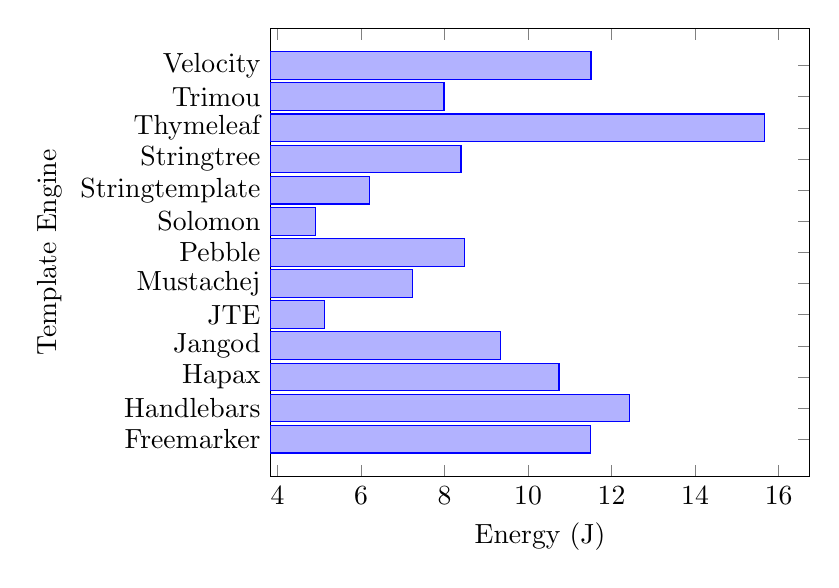
\begin{tikzpicture}
\begin{axis}[
    scaled ticks=false,
    % xmode=log,
    % ticks with fixed point,
    % scaled ticks=false,
    xbar stacked,
	bar width=10pt,
	% nodes near coords,
    ytick=data,
    legend style={at={(0.5,-0.20)},
      anchor=north,legend columns=-1},
    ylabel={Template Engine},
    xlabel={Energy (J)},
    symbolic y coords={
        Freemarker, Handlebars, Hapax, Jangod,
        JTE, Mustachej, Pebble, Solomon,
        Stringtemplate, Stringtree, Thymeleaf,
        Trimou, Velocity
    },
    ]
\addplot+[xbar] plot coordinates {
  (11.4936,Freemarker) (12.4403,Handlebars) (10.7424,Hapax) (9.33103,Jangod)
  (5.13393,JTE) (7.22679,Mustachej) (8.48842,Pebble) (4.90431,Solomon)
  (6.20053,Stringtemplate) (8.39519,Stringtree) (15.6721,Thymeleaf)
  (7.98896,Trimou) (11.5069,Velocity)
};
\end{axis}
\end{tikzpicture}
\caption{Net energy use for 1000 sets of scenarios by \gls{template engine}}
\label{fse:graph:net 1000}
\end{figure}

\subsection{Discussion}
\label{fse discussion}

The results from \autoref{fse:results:net 1000} show a discernible difference in energy usage between the \gls{template engine}s. However, the scale of the difference is considerably less than shown in the performance figures from \autoref{chapter:performance}. Also, the energy use figures from this experiment do not align well with the performance figures. A striking example is \emph{JTE}, which exhibited the slowest performance at 1000 repetitions of all the \gls{template engine}s in this cohort (see \autoref{set 4 overview}. According to the \enquote{folklore} described in \citep{Yuki2013}, slower performance implies longer running time, which implies greater energy use. However, this component shows the second lowest energy usage in this experiment.

While the energy usage figures from this experiment are interesting, they should not be considered authoritative for several reasons:

\paragraph{Low number of samples}
The typical duration of 1000 repetitions of the suite of template scenarios for these \gls{template engine}s was between 10 and 20 seconds. The experimental test apparatus was configured to sample current and voltage at 1 second intervals, which meant that each run only had 10-20 readings from which to derive an average energy figure [\autoref{fse2:energy single 1000}]. 

\begin{figure}[htbp]
  \centering
  % \def\svgwidth{\columnwidth}
  \includesvg[width=\columnwidth]{Figures/graphs/Energy/SingleRun1000.svg}
  \caption{Energy readings from 1,000 runs of \emph{Pebble}}
  \label{fse2:energy single 1000}
\end{figure}

\label{A204}
The readings varied during this period although, with a variance of 0.0367 and a standard deviation of 0.1917, most readings stayed relatively close to the mean of 2.3508 W. Despite this, there is clear evidence of \enquote{noise}, so it is entirely possible that one or two outliers, either high or low, could perturb the average.

\paragraph{System \enquote{noise} and other external factors}
\label{A206}
The contribution to the energy due to the components in these experiments is small compared to the energy usage of the system as a whole, including the energy needed to run the \emph{Lighttpd} server. Background processes and the general functioning of the systems required to support a modern operating system and its applications add \enquote{noise} to the measurements which can, on occasion, overshadow the energy usage of the components. Background processes were minimised during these experiments, leaving only those required to enable the operation of the software being tested. When combined with the low number of samples and the experiment being run only once for each \gls{template engine}, this also acts to reduce confidence in the comparison.

\paragraph{Unrepresentative scenarios}
The performance experiments in \autoref{chapter:performance} were designed to investigate the differences in behaviour of \gls{template engine}s in specific circumstances. In those experiments it made sense to repeat each specific scenario many times in order to amplify the differences and minimise the influence of external factors. If the intention is to obtain a directly applicable comparison between the energy usage of components when deployed to real applications, then a more representative scenario might be more appropriate.

\paragraph{Platform differences}
The performance experiments in \autoref{chapter:performance} were conducted on an Intel CPU running a 64-bit operating system, while the energy experiments in this section were conducted on the energy measurement apparatus, which uses an ARM CPU running a 32-bit operating system. Differences between the performance results for the two different platforms are explored in \autoref{section:perf dut}.

\subsection{Conclusions}
\label{fse conclusions}

The initial conclusions from this experiment were that there was an apparent difference in the energy consumption of the \gls{template engine} components when tested with the simple scenarios used for the performance comparisons, but further investigation was required. Further experiments would need to include a larger number of cycles within each run and the averaging of several runs to minimise the impact of system noise and other external factors as well as the construction of further, more representative, scenarios. These further experiments are described in \autoref{section:fse2} and \autoref{section:context energy}.


\section{More Samples and Averaging}
\label{section:fse2}

Following the approach taken in \autoref{section:fs1} and \autoref{section:perf dut}, a further energy comparison experiment was carried out in which each \gls{template engine} was exercised 10,000 times for each of the performance test scenarios. Both energy use and time taken to process the test scenario were recorded. Each set of 10,000 was repeated three times for each \gls{template engine} and the results were averaged to reduce the effect of system noise and interference.

\subsection{Results}
\label{fse2 results}

Increasing the number of repetitions of each template scenario served to reduce the variability of the energy readings in most cases. \autoref{fse2:energy single 10000} shows relatively consistent energy use during the measurement, with the addition of noise in a similar manner to the performance graph in \autoref{results:fullsolomon}.

\begin{figure}[htbp]
  \centering
  % \def\svgwidth{\columnwidth}
  \includesvg[width=\columnwidth]{Figures/graphs/Energy/SingleRun10000.svg}
  \caption{Energy readings from 10,000 runs of \emph{Pebble}}
  \label{fse2:energy single 10000}
\end{figure}

\paragraph{Energy Use}
\label{fse2 results energy}

\autoref{fse2:energy graph} shows the comparative energy use of the selected \gls{template engine}s with the centre dot representing the average of three runs and the range bars indicating maximum and minimum values. The graph clearly shows a wide variation in energy use between \gls{template engine}s for this scenario.

\begin{figure}[htbp]
  \centering
  % \def\svgwidth{\columnwidth}
  \includesvg[width=\columnwidth]{Figures/graphs/Energy/ComponentEnergy.svg}
  \caption{Averaged energy use by template engine}
  \label{fse2:energy graph}
\end{figure}

\paragraph{Time Taken}
\label{fse2 results time}

\autoref{fse2:time graph} shows the time taken for the experiments shown in \autoref{fse2:energy graph}. There is also a wide variation between these figures which has some similarity to the energy usage but also has some important differences. For example, \emph{Hapax} shows as faster than \emph{Jangod}, but achieves that speed at the expense of extra energy usage.

\begin{figure}[htbp]
  \centering
  % \def\svgwidth{\columnwidth}
  \includesvg[width=\columnwidth]{Figures/graphs/Energy/ComponentTime.svg}
  \caption{Averaged test duration by template engine}
  \label{fse2:time graph}
\end{figure}

\paragraph{Running Power Consumption}
\label{fse2 results power}

Having recorded both total energy use and time taken for each of the test runs, it became possible to derive the average running power consumption for each of the \gls{template engine}s by dividing the total energy used by the total time taken for each run. These derived values are shown in \autoref{fse2:power graph}.

\begin{figure}[htbp]
  \centering
  % \def\svgwidth{\columnwidth}
  \includesvg[width=\columnwidth]{Figures/graphs/Energy/ComponentPower.svg}
  \caption{Averaged running power by template engine}
  \label{fse2:power graph}
\end{figure}

\subsection{Discussion}
\label{fse2 discussion}

Unlike the improved performance experiments in \autoref{section:fs2}, the experiments that provided the energy and duration values in this section only represented a single quantity of requests. However, there is a clear variation between the evaluated \gls{template engine}s in both time taken and energy used. 

While the emphasis of this research is on comparing the energy used by different software components, the addition of performance measurements also enables investigation into the running power consumption of the different components and its potential use as an indicator of the relationship between performance and energy use. This relationship between energy use and time taken, as shown in \autoref{fse2:power graph}, is also different for the different \gls{template engine}s. In these results, \emph{Hapax} uses approximately twice the running power of \emph{JTE}. A component that uses less running power is not necessarily a better or worse choice than one that uses more, however. The important values for capacity planning are performance, which can be used to determine the number of machines required to serve a desired number of requests per second, and total energy use, which indicates which components are more or less energy-efficient for the same task.

The disparity in calculated running power, even at a single quantity of repetitions, indicates that performance measurement is a poor analogue for energy use. However, the combination of the different measurements can help decide which components to choose, at least for this kind of scenario on this kind of platform. For example, in this experiment, \emph{Velocity} exhibits both the worst performance and the worst energy use so is unlikely to be a good choice.\emph{JTE}, on the other hand performs consistently well in both performance and energy use. One concern with \emph{JTE} in this scenario is that it completes so quickly that it does not allow enough time for a large number of energy readings.

\subsection{Conclusions}
\label{fse2 conclusions}

This experiment confirms that there is an observable difference in both performance and energy use of different \gls{template engine} components. Combining the two sets of measurements also shows that the different components have different relationships between performance and energy use. This indicates that, without prior calibration specific to the code being executed, performance measurement is not a reliable way to predict overall energy use.

Results from \autoref{chapter:performance} showed that the different components perform differently under different volumes of requests, but the experiments in this section all used the same volume. It is expected that energy use, time taken, and running power will also vary depending on request volume.  Further experimentation is needed to validate this assumption as well as to determine how well such abstract test scenarios represent real deployments.

\section{Measuring Template Engines in Context}
\label{section:context energy}

\subsection{Introduction and Scope}
\label{cce intro}

The preceding experiments have concentrated on testing the behaviour of specific \gls{template engine} features. While informative, such scenarios may not be fully representative of the way such \gls{template engine}s are used on the web. To better simulate that kind of usage an example web page was converted to an intermediate template using the \emph{GILT} \gls{template language} discussed in \autoref{chapter:intermediate}. This intermediate template was then used to generate templates for a selection of \gls{template engine}s. The performance and energy usage of the selected \gls{template engine}s were compared using the apparatus described in \autoref{chapter:testrig}. The results of these comparisons are described in \autoref{cce results}.

\subsection{Methods}

\paragraph{Selecting A Web Page and Generating Templates}
\label{cce pages}

Web pages on the public internet vary widely. From simple pages holding a single image or a small amount of text to large, sprawling pages containing many distinct sections and structures. For the purposes of this investigation, a page was needed containing representative usage of many of the template features compared in previous sections. Such a web page would need boilerplate text, simple substitutions, template inclusion, iteration through a list, and boolean selection. Method invocation is not supported across the full range of \gls{template engine}s, so that was excluded from this investigation.

The desired set of features are found on many blogs and other similarly-structured sites. The blog page used for the comparison between servers in \autoref{chapter:testrig} only contains the content for a single page with little opportunity for iteration, so it was decided to use the \enquote{front page} of a blog that contains multiple tags, archive links, and sections for different blog posts. To avoid potential repeatability issues with relying on an externally-controlled website, a snapshot of the front page of the website and blog associated with this research\footnote{\url{https://greenprogrammer.net/}} was selected.

\paragraph{Generating Templates}
\label{cce gilt}

The aim of the experiment was to compare the performance and energy use of a range of \gls{template engine}s. In order to do this, templates would be needed in appropriate \gls{template language}s for each of the engines. The intention was to generate these templates from a single intermediate template coded using the \emph{GILT} intermediate language described in \autoref{chapter:intermediate}. It quickly became clear during the creation of this intermediate template that the only way to test for correctness was to generate a template for one of the candidate \gls{template engine}s and then expand that template using the appropriate \gls{template engine}. This process was cumbersome, and led to confusion whenever there was an error as to whether the issue was in the intermediate template, the template generation driver for the chosen target \gls{template language}, or the behaviour of the target \gls{template language} itself.

To eliminate some of these variables, and allow verification of the correctness of the intermediate template without using it to generate a template in a different \gls{template language}, a new \gls{template engine} was created. This \gls{template engine}, named \emph{gilt-native}, uses the \emph{GILT} intermediate language directly as its \gls{template language}. This \gls{template engine} enabled faster development and testing of intermediate templates without the need for third-party \gls{template engine}s and direct comparison of the expanded template with the expected web page. 
% Updated results graphs from \autoref{chapter:fs2} including the new \emph{gilt-native} \gls{template engine} are shown in \autoref{cce results}.

Once a intermediate template containing uses of all the desired features was complete, the \emph{GILT} template generator was used to generate appropriate templates for each of the \gls{template engine}s.

\paragraph{Selecting a Test Method}
\label{cce method}

When evaluating the effectiveness of the apparatus in \autoref{chapter:testrig}, web pages were served by a selection of servers using both dynamic (Wordpress) and static page data. When comparing performance and energy use of components in \autoref{section:fse} and \autoref{section:fse2}, each test scenario was invoked directly using a script. Both approaches showed clear differences between energy use but in the server-based tests the differences between server implementations had the potential to overshadow the differences between components. In order to directly compare the performance and energy use of the candidate \gls{template engine}s it was decided to run each engine from a script in a similar manner to the component tests.

Scripts from the separate scenario tests were copied and modified to load appropriate context data and invoke each \gls{template engine} using its \verb!EngineDriver! implementation using its generated template.

\paragraph{Evaluating the Template Engines}
\label{cce evaluation}

Prior to use on the measurement apparatus, each \gls{template engine} was invoked with the intended context data and generated template, and the result was compared with the expected web page. This highlighted several problems that needed to be addressed before the performance and energy use of the \gls{template engine}s could be measured and compared.

The most common problems were differences in the handling of \enquote{whitespace} such as space, tab, and newline characters. All the \gls{template engine}s in this cohort were designed primarily to generate output formatted using HTML. The rendering of HTML by web browsers is mostly insensitive to the presence or absence of such whitespace, so the \gls{template engine} developers have not always cared about exactly preserving whitespace when generating web pages. For example, \emph{velocity} failed to preserve a new line following a template inclusion directive (see \autoref{velocity diff}).

\begin{figure}[htbp]
  \centering
  \includegraphics[width=\columnwidth]{Figures/graphs/Page/velocity-diff.png}
  \caption{Difference in generated whitespace}
  \label{velocity diff}
\end{figure}

After examining the output from these \gls{template engine}s, the acceptance criteria for a successful template expansion were relaxed to allow such minor differences in whitespace.

Other \gls{template engine}s, however, had bigger issues. Even though each of the \gls{template engine}s considered for this phase of the investigation had passed the individual tests in \autoref{chapter:performance}, some failed to generate acceptable output for this more complex scenario. For example, \emph{Solomon}, which had performed flawlessly on the individual scenarios, initially generated a much smaller output file than the other \gls{template engine}s. When the output was examined it was clear that the template inclusion directives had failed. To understand why this was happening, the source code for the \emph{Solomon} \gls{template engine} was used instead of the provided library, and instrumented to discover the cause of the problem. An issue was discovered in the filenames of the templates to be included. \emph{Solomon} expected the names of included templates to conform to the rules for identifier names in Java: starting with a letter then containing a combination of letters, digits, \verb!_! and \verb!$!. The filenames of the blog post summaries to be included had names beginning with their creation date in the form \verb!2022-10-23! which meant that the filenames were not valid Java identifiers. Once this issue was resolved, by renaming included template file to be valid Java identifiers, \emph{Solomon} generated the correct output. This issue was subsequently addressed in a later release of \emph{Solomon}.

Of the remaining \gls{template engine}s, some initially  failed to process the generated template at all.

\emph{JTE}, which had performed well in the tests of individual features, uses an approach that converts a supplied template into Java source code, then compiles that source code and runs it to expand the template. This approach requires additional specialist annotation in templates to enable the correct Java code to be generated. Unlike all the other \gls{template engine}s, which provide access to data values via a shared context visible to all templates, \emph{JTE} requires that context value names and types be declared in a header section at the start of the template. When including one template in another, any context values used in the child template need to be both declared in the child template, and passed as \enquote{parameters} in the include directive. During the evaluation of individual \gls{template engine} features and the development of the \emph{JTE} driver, no child template made use of context values, so this requirement was never discovered. Although the \emph{JTE} driver generated child templates with the correct declarations, it failed to generate the correct \enquote{parameters} in the parent template, which in turn meant that \emph{JTE} generated invalid Java code that \emph{JTE} could not compile. To add this feature to the \emph{JTE} driver would require the template generation code to model the complete, transitive, contents of every child template in order to generate a correct parent template. This would require major changes to the architecture of the template generator, so \emph{JTE} was excluded from this phase of the \gls{template engine} evaluation.

\emph{Stringtemplate} also required included templates to be valid Java identifiers but, even after the names of included templates had been adjusted as for \emph{Solomon}, the template generation process still produced invalid templates. Further investigation determined that the \emph{Stringtemplate} driver was using incorrect delimiters for some situations. The driver was updated to correct this error, and then \emph{Stringtemplate} correctly processed the generated template.

\emph{Handlebars} crashed when attempting to expand the generated template. Investigation indicated that this was a problem with the specific version of the \emph{Handlebars} library that was being used, which made use of some features incompatible with recent versions of Java\footnote{\url{https://github.com/swagger-api/swagger-codegen/issues/10966}} \footnote{\url{https://teamtreehouse.com/community/broke-when-adding-blocks}}. Updating the library removed this problem, but revealed further issues. All previous comparisons had been performed with a single version of the \emph{Handlebars} library. Updating to a new version, even if the further issues could be addressed, would raise questions about the comparability of the measurements, so \emph{Handlebars} was also excluded from this phase of the \gls{template engine} evaluation.

\emph{Mustachej} required some minor changes to the Driver, but otherwise functioned correctly.

\emph{Hapax} does not fully support loops and conditionals, so was excluded from this phase of the \gls{template engine} evaluation.

\emph{Thymeleaf} employs an HTML-specific syntax that would require altering the intermediate template document in ways that would make it incompatible with the other \gls{template engine}s, so it was also excluded from this phase of the \gls{template engine} evaluation.

Energy and performance comparisons were therefore performed on the following \gls{template engine}s:
\emph{trimou},
\emph{solomon},
\emph{freemarker},
\emph{stringtemplate},
\emph{stringtree},
\emph{jangod},
\emph{velocity},
\emph{pebble},
\emph{mustachej},
and \emph{gilt-native}.

A script was created to load a specified context and use a single \gls{template engine} to expand the templates generated from the example website. Each page expansion was run 100,000 times. The overall run of 100,000 expansions was then repeated twice more, and the results averaged, to minimise the impact of external interference.

\subsection{Results}
\label{cce results}

The energy usage of the averaged runs for each \gls{template engine} are shown in \autoref{cce:energy page 100000} and the time taken by each \gls{template engine} is shown in \autoref{cce:time page 100000}. These two data sets have been combined to produce running power figures for each \gls{template engine}, and these results are shown in \autoref{cce:power page 100000}

\begin{figure}[htbp]
  \centering
  % \def\svgwidth{\columnwidth}
  \includesvg[width=\columnwidth]{Figures/graphs/Page/Full-Page-Energy.svg}
  \caption{Energy usage of 100,000 page expansions}
  \label{cce:energy page 100000}
\end{figure}

\begin{figure}[htbp]
  \centering
  % \def\svgwidth{\columnwidth}
  \includesvg[width=\columnwidth]{Figures/graphs/Page/Full-Page-Time.svg}
  \caption{Time taken for 100,000 page expansions}
  \label{cce:time page 100000}
\end{figure}

\begin{figure}[htbp]
  \centering
  % \def\svgwidth{\columnwidth}
  \includesvg[width=\columnwidth]{Figures/graphs/Page/Full-Page-Power.svg}
  \caption{Average running power for 100,000 page expansions}
  \label{cce:power page 100000}
\end{figure}

\subsection{Analysis}
\label{cce analysis}

In \autoref{cce:energy page 100000} there is an observable difference between the energy usage of the different \gls{template engine}s. There is also a clear distinction between two groups of \gls{template engine}s: those which use less than 100J, and the four \gls{template engine}s that consume over 350J for the same scenario. This distinction suggests that there is some key aspect of the design or implementation that differs between the two groups. Investigation of the reason or reasons for this difference is out of scope for this research, but such a large difference could indicate a potentially fruitful area of future research (see section:future work).

The times taken shown in \autoref{cce:time page 100000} largely echo the energy usage results, with the same four \gls{template engine}s taking the longest to process the specified number of template expansions. The relationship between the \gls{template engine} energy usage and duration is not constant, however. For example, when considering only energy usage, \emph{velocity} is noticeably worse than \emph{stringtemplate}, but for time taken, these positions are reversed. This difference can be clearly seen in \autoref{cce:power page 100000}. \emph{velocity} uses more energy in a shorter time, which shows as a much higher running power consumption.

While the power figures in \autoref{cce:power page 100000} can be useful when comparing components whose energy usage and time taken are roughly similar, they are not indicative of any notion of efficiency. \emph{mustachej}, for example, shows by far the highest running power consumption, but is still among the lowest for total energy consumption and time taken to complete the task.

\section{Discussion}
\label{ce duscussion}

This chapter has explored some different ways of comparing the energy usage of \gls{template engine} components. Comparing software components is challenging because, unlike full applications, they cannot be executed without other software to configure, initiate, execute, and shut down the components. This external software can potentially influence the time and energy performance of the components. The results in this chapter show that software components do not usually perform identically in different scenarios. 

The experiments have shown clear differences in energy usage between \gls{template engine} components. The combined individual scenario experiments in \autoref{section:fse2} provide a ranking of \gls{template engine}s by energy usage as shown in the first data column of \autoref{ce rankings}. If considered in isolation, this ranking would seem to provide a way to select the most energy-efficient \gls{template engine} for a project. However, when the same \gls{template engine}s were compared using the arguably more realistic scenario of generating a complete web page, the rankings were very different as shown in the second data column of \autoref{ce rankings}.

\begin{table}[ht]
\centering
\begin{tabular}{lrr}
\multirow{2}{*}{Template Engine} 
      & \multicolumn{2}{c}{Energy Efficiency Ranking} \\
& Individual Scenarios & Full Page Generation \\
\hline
freemarker & 8 & 3 \\
gilt-native & \emph{n/a} & 8 \\
handlebars & 9 & \emph{n/a} \\
hapax & 11 & \emph{n/a} \\
jangod & 10 & 6 \\
jte & 1 & \emph{n/a} \\
mustachej & 2 & 5 \\
pebble & 6 & 2 \\
solomon & 3 & 1 \\
stringtemplate & 4 & 7 \\
stringtree & 7 & 10 \\
thymeleaf & 12 & \emph{n/a} \\
trimou & 5 & 4 \\
velocity & 13 & 9 \\
\end{tabular}
\caption{Comparative energy-efficiency rankings for all template engines\label{ce rankings}}
\end{table}

\label{IN24}
To examine the correspondence between these two sets of rankings, a Kendall Rank Coefficient (also known as Kendall's $\tau$) was calculated. This measure is a non-parametric hypothesis test for statistical dependence and produces a value between -1 and 1, with positive numbers indicating greater correspondence and negative numbers indicating lesser correspondence.

However, this calculation is complicated by the incomplete nature of the two sets of rankings. Kendall's test requires directly comparable sets of rankings, so the data needed to be adjusted to achieve this before the statistical test could be performed. There was no problem with the rankings for template engines that appear in both lists, but template engines that only provided rankings for one of the comparisons have no obvious position in the rankings for the other.

Four approaches to address this issue were considered:

\begin{itemize}
\item replace missing values with a low or out-of range value, such as 0 or 1
\item replace missing values with a high or out-of range value, such as 13 or 14
\item replace missing values with a middle or average value
\item remove template engines with missing values from the comparison.
\end{itemize}

The high and low approaches were rejected as they would skew the results of the test and reduce the confidence in the calculated value. The middle or average approach, while potentially having less impact on the calculated result, would also invalidate the calculation, as the Kendall Rank Coefficient assumes distinct ranking values. As a result, only templates with ranks for both the individual scenarios and the full-page generation were considered for the comparison. Removing rows where one side or the other was missing left some gaps in the rankings. These gaps were closed by moving adjacent rankings down until both columns contained only the numbers 1 to 9.

The final list of template engines, with their adjusted rankings, is shown in \autoref{ce rankings exc}.

\begin{table}[ht]
\centering
\begin{tabular}{lrr}
\multirow{2}{*}{Template Engine} 
      & \multicolumn{2}{c}{Energy Efficiency Ranking} \\
& Individual Scenarios & Full Page Generation \\
\hline
freemarker & 7 & 3 \\
jangod & 8 & 6 \\
mustachej & 1 & 5 \\
pebble & 5 & 2 \\
solomon & 2 & 1 \\
stringtemplate & 3 & 7 \\
stringtree & 6 & 9 \\
trimou & 4 & 4 \\
velocity & 9 & 8 \\
\end{tabular}
\caption{Adjusted rankings for template engines that participated in both studies\label{ce rankings exc}}
\end{table}

The adjusted rankings were then able to be used to generate a Kendall Rank Coefficient ($\tau$) of 0.277.
The $\tau$ value is positive, indicating that the two sets of rankings are more correlated than they are un-correlated.

However, taking as a null hypothesis that the two sets of rankings are independent, which would produce a $\tau$ value of 0, this results in a $p$ value of 0.358, which is low, but not low enough to reject the null hypothesis completely.

\label{A212}
The use of the GILT template generation software was an enabler for these experiments but did not figure in the measurements themselves. All GILT processing took place to generate all the templates before any timing or energy experiments were run. This use of an \gls{eager evaluation} approach removed the time and energy required for the GILT processing from the software being measured. The main benefit of using the GILT software was that it enabled easier interchangeability of template engine components by removing the dependency on manual editing of different template formats.

\subsection{Comparisons With the Performance Studies}
\label{ce performance}

The performance studies in \autoref{chapter:performance} could also potentially be used to rank the \gls{template engine} components based solely on performance. However, these experiments revealed that the various \gls{template engine}s exhibit different performance characteristics based on the overall volume of requests. Any potential rankings based on the performance studies of individual \gls{template engine} features would only be valid for the specific features being evaluated at that particular request volume. The energy comparisons were performed at fixed request volumes in order to gain a workable number of energy usage samples, but it is expected that energy-efficiency of some \gls{template engine}s would also vary with request volume.

\subsection{The Relationship Between Energy Use and Performance}
\label{ce relationship}

For the components evaluated in this chapter, the relationship between energy usage and time taken was neither constant between \gls{template engine}s nor constant between scenarios. This relationship, formulated as average running power is shown in \autoref{fse2 results power} and \autoref{cce:power page 100000}. In both scenarios the ratio between energy use and time taken, expressed as Joules per second (Watts) ranged from under 0.3 W to around 0.6 W. This variability suggests that models which aim to predict energy usage based on time performance are unlikely to be generally applicable.

\section{Conclusions}
\label{ce conclusions}

The key conclusion drawn from the experiments in this chapter is that different software components can vary widely in both energy usage and performance when performing the same task, and that the relationship between performance and energy usage is not constant across different evaluation scenarios. 

One implication of this is that models which attempt to predict energy use solely from other measurements such as performance, task complexity, or static analysis of code will not yield generally-applicable results. However the results affirm the importance of measuring actual performance and energy usage during system tests as an effective way to compare energy use between software changes. The apparatus described in \autoref{chapter:testrig} can enable this testing as part of the regular software development and automated testing process.

\chapter{Conclusions}
\label{chapter:conclusions}

\section{Reflection}
\label{conclusions:reflection}

Environmental sustainability is one of the major challenges of the modern world. We need to immediately and significantly reduce the production and emission of greenhouse gases. Energy production, driven by energy consumption, is a major contributor to greenhouse gas emissions. The energy consumption of the world's \gls{ICT} systems is a significant contributor to global energy demand.

This research has explored ways to improve the sustainability of large-scale \gls{ICT} systems by reducing energy consumption and its associated greenhouse gas emissions. Most \gls{ICT} systems are controlled by software that has the capacity to increase or decrease the required energy. Software systems are created and maintained by software developers in the context of existing software and infrastructure, organisational culture, and personal skills. Exploring this context of software development gave insight into many reasons why energy efficiency and the sustainability of software systems are often not a high priority.

The literature on computing and sustainability revealed \enquote{vague, diverse and contradictory ideas} and confusion between subdisciplines. Several research teams have released manifestos or proposed frameworks in an effort to clarify the state of sustainable computing research, but there is little evidence of this extending beyond academia.

A research gap was identified in the use of component substitution to reduce the energy use of large web software, and web template systems were selected as a representative category of component for investigation. A general lack of information on the performance and energy usage of these components was identified, so a series of experiments were carried out to discover the feasibility and effectiveness of component substitution as a sustainability strategy.

A feasibility study was conducted to determine whether the scale of differences between a selection of template components was large enough to warrant further investigation. The results of this study indicated that the fastest component (\emph{Solomon}) was, on average, 2642 times faster than the slowest (\emph{Casper}). Further performance comparisons were performed that showed that although individual component performance varied depending on task and load, there were still considerable differences in performance between components. Selecting components with better performance could therefore potentially reduce the number and/or capabilities of computers needed to run a popular service, thereby reducing both energy usage in operation and the embodied carbon costs of manufacturing and disposal of the hardware.

Although optimising performance can help reduce hardware requirements, it is not a direct measurement of energy use. A prototype test apparatus was designed and constructed to support automated, programmable, comparison of the energy used by applications or software components under different scenarios and loads. Comparisons using the apparatus produced some interesting results, including that the popular \emph{WordPress} application used by a very large number of websites requires a lot more energy to serve each web page than an equivalent traditional \enquote{static} website.

The feasibility of component substitution as a strategy depends on the cost and complexity of replacing one component with another. However, software components provide individual APIs and are rarely directly interchangeable. To explore potential solutions to this problem, a framework was constructed to simplify the creation of \enquote{drivers} for different component APIs. Components can also differ in data formats and data storage requirements. To explore this issue, an intermediate data format and associated conversion tools were created to simplify the generation of appropriate data for each component. This combination of framework, data format, and tools was then used to create more complex scenarios to evaluate the energy consumption of the selected template components. The results showed that there was also a considerable difference in energy consumption between components, although this did not always align with the performance of the components. 

The implication of this research is that replacing software components with alternatives with better performance can potentially help improve sustainability. However, performance on its own is not a good proxy for operational energy usage.

A more effective and direct way to assess and reduce the energy usage of a software system is to use an energy comparison apparatus, such as the prototype developed as part of this research, to include energy usage comparison in existing automated test suites. This approach would allow comparisons of energy usage to be performed in load and deployment scenarios customised to the needs of the software in use.

\section{Evaluation of Research Objectives}

A set of research objectives were described in \autoref{section:research objectives}. This section examines the outcomes and evaluates the effectiveness of this research against these objectives.

\subsection{Investigate the context of web software and its development}

Research was conducted on the scale of the internet, the history of computing, and how software is made, including development team roles and how software developers choose components. It was discovered that many forces act to prioritise other goals than sustainability. Improved education, reliable information, and energy measurement tools that fit in with existing development processes are required to enable software developers to improve the sustainability of the software being produced or maintained.

\subsection{Explore the differences in performance of a selection of template engine
components}

A representative category of software component was selected and a small cohort of implementations was chosen from within that category. A software performance test harness was created for a feasibility study to explore the performance of the implementations in a range of scenarios. This initial feasibility study clearly indicated large performance differences between these components and demonstrated that the area was worthy of further study. However, there were some issues with the interaction between the performance test harness and the components being evaluated.

An improved performance test harness was constructed to address the issues raised by the feasibility test. A driver framework was created to allow independent loading of \gls{template engine} components into the comparison framework. A new component could be added and compared by writing a driver for the new component with no need to modify or recompile the comparison framework. The comparison framework was used to compare both component performance and (when used with the energy test apparatus) component energy usage.

This confirmed the large differences in component performance found in the feasibility study and also discovered that component performance varies not only between components and scenarios but also between the volume of requests.

This research was effective in showing that there are ways to simplify the complex and potentially expensive task of comparing software components. The development of standard tools for performance and energy usage comparison as well as tools to overcome the differences in component APIs and data formats has helped compare the performance and energy-use differences between components. With the ability to compare components comes the ability to select ones with better performance and lower energy use. This, in turn, could lead to an overall reduction in energy use and associated carbon emissions.

This research was also effective in uncovering the scale and complexity of the performance differences between supposedly-equivalent software components. This stands in sharp contrast to the documentation and other public information available about these components. Such documentation rarely mentions performance, and when it does it is usually in vague terms such as \enquote{fast} or \enquote{powerful}. Using this information to select components with optimum performance for a desired application could potentially reduce the number of computers needed to serve that application, thus reducing the embodied carbon in the system.


\subsection{Construct a test apparatus to compare the energy use of software during operation}

An apparatus was designed, constructed, and evaluated to assess the energy usage of running software under different scenarios. This phase of the research was very successful, resulting in a useful apparatus that was then used for subsequent experiments.

This research was effective in showing that an apparatus could be constructed to compare the energy usage of both components and whole applications in a variety of scenarios. Importantly, this apparatus was built for much less cost than traditional lab equipment and provided software interfaces so it could be included in the \gls{continuous integration} processes commonly used to test software during development. Comparisons run on the apparatus revealed the wide range of differences in energy consumption between equivalent software, in particular, the much larger energy required to serve websites using WordPress software.


\subsection{Use the apparatus from \autoref{chapter:testrig} to compare the energy use of common
web software and the feasibility and effectiveness of substituting template engine components}

The energy comparison apparatus was used to compare the energy usage of a selection of popular web server applications, both when serving static and dynamic web pages. The results of this comparison clearly showed not only a difference in energy usage between servers but also highlighted the large hidden energy cost of dynamic website generation.

An intermediate language was designed to represent common features of \gls{template language}s and a software tool was constructed to convert templates expressed in the intermediate language into the various formats required by different \gls{template engine}s. The template generation tool also used a driver mechanism, allowing new \gls{template language}s to be added without the need to modify the generation tool. This intermediate language and tool were successfully used to generate representative web page templates for \gls{template engine} comparisons, based on a real website, for each of the supported \gls{template engine}s.

The cohort of software components that had been compared for performance was then compared for energy use. Energy use was compared both when re-running the performance evaluation scenarios and when running new scenarios designed to be more representative of common use. The results of this comparison showed differences in the energy usage of the components but the relationship between performance and energy usage was different for each of the components.

The ability to compare both performance and energy usage of the same software highlighted the differences in the relationship between the two metrics. Although many attempts have been made in the literature to derive ways of using performance to predict energy usage, this research clearly showed that the relationship between the two varies both between components and between usage scenarios. Any models which claim to relate the two metrics will therefore only be of use in very limited circumstances.


\subsection{Research Objectives Conclusions}

Of the four research objectives, three were very successful, providing a range of contributions to knowledge that should help improve the sustainability of software systems. The objective of investigating the context of web software and how it is developed confirmed existing concerns about the lack of support for the development of sustainable software. There is increasing interest in this area by academic researchers, but this does not appear to have had much influence on existing software development practices. However, that research did provide the justification for exploring ways to improve the sustainability of software systems through other means that do not require rapid changes to the practices, structure, and roles of software development teams.


\section{Contributions To Knowledge}
\label{section:contributions}

This research has generated several contributions to knowledge, which are described below.

\subsection{A Novel Self-Contained Apparatus for Comparing Software Performance and Energy Consumption}
\label{contrib:apparatus}

While there have been several studies that have measured or compared the energy usage of software, they typically involve expensive laboratory equipment or manual measurements, require specific computer hardware, or concentrate on the investigation of theoretical models rather than enabling energy measurement and comparison as part of routine software development and testing.

This research has developed a self-contained, low-cost prototype for an apparatus that can be integrated into the automated \gls{continuous integration} processes used by many industry teams when developing and testing software. The apparatus can operate without human intervention to compare the performance and energy use of a wide range of software applications and software components with customisable scenarios and load levels. The apparatus is designed to integrate with automated test systems, but also offers a manual web interface, which can be useful when evaluating candidate software to include in a project.

\subsection{Energy Use and Performance Comparisons for a Cohort of Web Server Implementations}
\label{contrib:servers}

The apparatus described in \autoref{chapter:testrig} was evaluated by comparing the energy use and performance of a variety of web server implementations, including two of the most widely used servers worldwide, to serve some representative web content. The results clearly indicate the differences between the implementations. This information is not available elsewhere.

\subsection{The Relative Energy Usage of WordPress Compared to Static Websites}
\label{contrib:wordpress}

\emph{WordPress} is a very popular tool for creating, managing, and serving websites, yet users are mostly unaware of its energy consumption. This research has revealed that \emph{WordPress} requires many times more energy to serve the same web pages compared with a traditional \enquote{static} website. Although \emph{WordPress} can provide website features that static sites cannot, these features are not used by all \emph{WordPress} websites. There are a potentially large number of websites currently running \emph{WordPress} that could be switched to a static approach for an immediate saving in energy.

\subsection{A Novel Extendable Java Framework for Template Engine Comparison}
\label{contrib:framework}

Selecting a \gls{template engine} component for a project can be a daunting task. The lack of detailed information provided by the component creators leads to a choice between committing to one component (and hoping it is a good choice) or conducting comparative experiments. The construction of rigorous comparative experiments can be complex, but that complexity can be reduced using the \gls{template engine} comparison software framework constructed for this research. When using this framework all that is needed is to define the template scenarios to be tested and write driver implementations to suit the API of each candidate \gls{template engine}. The framework takes care of dynamically loading the correct drivers and templates, running the selected scenarios, and collecting results ready for analysis.

\subsection{Energy Use and Performance Comparisons for a Cohort of Template Engine Implementations}
\label{contrib:engines}

As part of this research, the comparison framework described in \autoref{chapter:performance}, the intermediate language described in \autoref{chapter:intermediate}, and the apparatus described in \autoref{chapter:testrig} were utilised to compare the energy usage and performance of a cohort of open source \gls{template engine}s of the kind commonly used for the generation of dynamic web pages. These comparisons involved multiple platforms and a range of scenarios and load levels. This information is not available elsewhere.

\subsection{A Challenge to the Notion of Execution Speed as a Proxy for Software Energy Usage}
\label{contrib:speed as proxy}

It seems to be a common opinion, even being referred to as \enquote{folklore} in one paper \citep{Yuki2013}, that energy usage of software is in some way related to the time taken to accomplish a task. Many researchers have attempted to construct models to relate the two quantities in the hope that relatively simple and cheap performance measurements could be used to produce an estimate of energy usage. This research has shown that when evaluating a range of software that performs a broadly similar task, there is no constant or reliable relationship between execution speed and energy use. Different components have different relationships, which vary between different evaluation scenarios.

This research leads to the conclusion that the only practical and effective way to compare the energy use of software in operation is to measure it.

\subsection{A Challenge to the Notion of Task Complexity as a Proxy for Software Energy Usage}
\label{contrib:complexity as proxy}

Many works on the topic of software energy usage have made the implicit or explicit assumption that the energy use of a software system is primarily dependent on the complexity of the task the software system performs. This may be true in cases where there is a very large difference in task complexity. In such cases, reducing the complexity of the task is likely to reduce overall energy usage. However, this research has shown that the architecture and design of the software to perform the task can also make a big difference, even when the task being performed is the same.

\subsection{The Efficacy of Component Substitution as a Strategy to Improve Software Sustainability}
\label{contrib:efficacy}

This research has discovered major differences in the performance and energy use of different software components when performing similar tasks. This clearly indicates that the choice of software components, when designing a new system or modifying an existing system, could be a viable strategy to improve the sustainability of software.

\section{Future Work}
\label{section:future work}

Each of the studies in this research has also revealed the potential for further work.

\subsection{The Performance of Software Components}

The performance of software components under real conditions is an under-researched area. Historically, academic research has concentrated on the study of algorithms and data structures, but such abstract concepts are less-often considered in practical software development. Instead, software architects and developers attempt to design and construct systems from components, but lack detailed information to use when selecting between many candidate components. Although a poor proxy for energy use, in general, component performance comparisons can assist in designing software systems that require fewer or less powerful computer hardware systems to support them.

Within the category of \gls{template engine}s, more research is needed to investigate the design and characteristics of the selected components to investigate why their performance is so different, and to determine if any software development or evaluation guidelines can be derived from this information.

The generally similar performance of the embedded web server components seen in \autoref{servers:analysis}, despite their different implementations and energy use, is also an anomaly which would benefit from further investigation.

This research has concentrated on one specific type of component, but there is a very broad range of software component types available, many of which also have a large number of substitution candidates. Further research is needed on the performance of other types of software component to investigate whether the results from this research are in any way representative.

Further research would also be useful on the impact on application performance of including multiple components and the possibility of models that could predict or estimate overall performance or hardware requirements from a \enquote{software bill of materials}.

Most research in this area is limited by a lack of information, so there is also potential for future research to find ways to grow the range, detail and reliability of information available on software components. An approach to this might be to develop tools and benchmarks that can be used to compare components. For \gls{template engine} components these might take the form of standardised template scenarios that can be applied to many candidate \gls{template engine}s.

\subsection{An Apparatus To Compare Energy Usage}

The energy comparison apparatus developed in this study was only a prototype and thus there is ample opportunity for further research and development. Potential research areas include:

\begin{itemize}
    \item evaluating the use of alternative \enquote{DUT} platforms to better simulate the hardware used in commercial applications.
    \item evaluating or developing different energy measurement circuits that can handle larger voltages and currents.
    \item improving the software to support multiple scenarios in a single test run.
    \item improving the software and database to support the parallel operation of more than one apparatus.
    \item evolving the apparatus into a robust, self-contained device.
    \item investigating and constructing tools to help integrate the apparatus with specific software \gls{continuous integration} systems.
    \item enhancing the output and presentation of comparison results to better inform decision-making
\end{itemize}

Further research is also needed in the broader field of software energy usage measurement and communication. The results of the energy usage of different software applications and components need to be disseminated so that potential users can make an informed decision without always having to perform their own comparisons of energy usage. This in turn would need standards and repeatable methodologies as well as devices such as this apparatus.

\subsection{Substitution of Incompatible Software Components}

The software developed as part of this investigation to support the substitution of components that are partly functionally equivalent but provide different APIs and data formats was specific to \gls{template engine} components, but the approach is potentially applicable to other classes of components. More research would be required to determine how broadly applicable this approach is to other contexts.

\subsection{The Energy Use of Software Components}

The performance results of the evaluation of \gls{template engine} components using the comparison apparatus in \autoref{chapter:comp energy} are interesting, but do not align well with the performance results of the studies in \autoref{chapter:performance}. The measured values were expected to be different from the previous experiments as they were executed on different computers with different processors. However, what was not expected was that performance \emph{rankings} would be so different. There is clearly something else different about the two platforms, which needs further investigation.

The difference in performance rankings raises questions about the accuracy of the energy use comparisons and rankings for the same scenarios. These also need to be investigated, ideally in a range of different request volumes as was done for the performance studies in \autoref{section:fs2}. 

\subsection{Other Related Future Research}

This research has continually shown that there is a lack of detailed and reliable information about software in general, but in particular about software components. Electrical appliances have energy ratings, electronic components have data sheets, but software components mostly have little more than feature lists and usage instructions at best. Further research is needed into ways to obtain, share, and compare information about the characteristics of software components.

The comparisons of server energy use in \autoref{chapter:testrig} highlighted the poor performance of dynamic websites and, in particular, \emph{WordPress}. Further research is needed on the development of software that can make the management of static websites as easy and flexible as \emph{WordPress} but without the high energy cost.

\section{Final Remarks}

As mentioned at the very beginning of this dissertation, this PhD was motivated by concern for the future of our environment. This research has revealed the increasing environmental impact of computing technology and with it the importance of improving the sustainability of software-driven computing. The experimental results of this research have shown that the environmental impact of both software applications and software components can be reduced by choosing alternatives with better performance and/or better energy efficiency and by improving the process of software development to include these aspects alongside other requirements and document them alongside other features.

As a researcher and the author of this dissertation, I earnestly hope that this work will make a positive difference.

% \chapter{Context Of This Research}
\label{chapter:context}

\section{The Scale of The Internet}
\label{section:context scale}

The modern world contains a vast number of electronic devices. The emphasis of this research is on the development of software, so the scope of this research will be limited to devices and systems which include software as a key element. Software is more pervasive, and more complex, than many people think \citep{Kang2015}, though, with software controlled devices ranging from the barely visible and commonplace to multi-million-dollar and planet-wide systems. There are even thousands of computers in space, as they form a key part of every modern spacecraft and artificial satellite \citep{Eickhoff2011}. Increasingly, even small devices, sensors, or appliances include network connectivity and collaborate both with each other and with more traditional computer resources to form the so-called \emph{internet of things}. The internet is already by far the largest and most complex computer system ever built, and every addition makes it even bigger \citep{Belkhir2018}. 

It's hard to get to grips with the scale of the \gls{internet} because so much of it is behind-the-scenes, The most visible aspect of the internet is the \gls{web} (also known as the `www', or just `web'). This may seem relatively simple, because a user can only see at most a few pages at a time, and most people stick to familiar high-profile shopping, social, and informational websites \citep{Similarweb2023}. The web is a \gls{distributed system} consisting of many communicating devices. As originally conceived \citep{Berners-Lee1992} the web was a purely \gls{client-server} system.

Anyone wishing to find some information would use a textual interface or a \gls{web browser} such as the original \emph{NCSA Mosaic} software \citep{Strawn2014} or one of its conceptual descendants such as \emph{Chrome}, \emph{Firefox}, \emph{Edge}, or \emph{Internet Explorer} (which function as the \gls{client}) to request and receive information from one or more data storage machines (known as the \emph{servers}). This is still essentially how the web works today, although extra complexity has been added in the decades since the web's initial design.

Estimates vary as to the `size' of the web and many different approaches have been taken to try and come up with an answer, from random IP-address probing \citep{Xing2003} and undisclosed proprietary algorithms \citep{Murray2000} to lurid websites with unclear data sources\citep{LiveCounter2018}. A slightly more trustworthy estimate is provided by \citet{Worldwidewebsize2018} which at least explains its methodology and data sources \citep{Kunder2008}. This website (at time of writing, 18 March 2024) reports \enquote{at least 5.22 billion pages}. It is important to note, however, that \citet{Worldwidewebsize2018} uses a mechanism based on search engine results and is therefore unable to count unindexed pages such as private (\gls{intranet}) sites, databases, and the so-called `\gls{dark web}'. The real figure is likely to be much larger. A different 2023 survey reported just over a billion websites running on a little over 12 million servers \citep{Netcraft2023} but made no claims about the number of web pages on each site.

As well as being \emph{big}, the web is also very \emph{busy}. There are billions of client devices and many web servers handle millions of requests per day \todo{citation?}. The growth of the \gls{internet of things} is increasing this even more as sensors and other `smart' devices send and receive data without ever involving a human being. Although often described naively as `\gls{the cloud}', the infrastructure of the internet is very physical. Every web request and response passes through a large network of devices including routers, switches, caches, transmitters, receivers, and signal boosters. Each of these contains electronics and the great majority of them also contain software.

A key to understanding the enormous numbers involved is that there is a \emph{lot} of duplication. Many web requests are for the same popular pages, and many pages are very similar to others. The well-known shopping website Amazon.com, for example, currently offers over 350 million products \citep{SellerApp2023}. To make this possible, Amazon uses a set of standard structures for its product pages, with each page differing only in details related to the specific product. The rest of the page is largely the same, with the same branding, layout, headers and footers and so on. Many very high traffic websites need to run multiple servers serving the same website to handle the load, resulting in even more duplication.

Although an increasing amount of the modern web involves some code which runs on the device with the web browser (known as \gls{client-side processing}), the great majority of the work of the web is done on the servers which provide the web browsers with their data. Servers are responsible for listening for requests from browsers using the \gls{http} protocol \citep{rfc2616} or the more secure but otherwise similar \gls{https}, and serving the correct responses. This process can be as simple as generating an error message or locating a stored file and sending the contents in response, or it can involve complex textual and numeric processing, reading multiple files, and collecting data from other servers and databases, before combining the result into a web page or other document ready to return to the client browser.

The huge scale of the internet results in a correspondingly huge consumption of energy. ICT devices and systems require a variety of forms of energy to operate including specific voltages to run micro-circuitry, power to move and spin mechanical parts, and electricity to run cooling fans, illuminate displays, and communicate with other devices. Active web servers are usually located in \gls{datacenter}s, where they have access to the physical security, power, cooling, and connectivity that they need. A single datacenter will often consume the order of tens of megawatts. This would be enough to power thousands, or even tens of thousands, of homes \citep{Law2022}.

Electrical energy consumption contributes to \gls{global warming} in several ways. The most direct is the generation of heat when the electricity is used to perform work. This heat is released into the surrounding environment causing localised warming. Most ICT equipment works best within a relatively narrow temperature range, and if the temperature around the equipment gets too high it needs to be cooled. This in turn requires more electrical energy. While the cooling process may reduce the temperature of the sensitive equipment, it also results in the release of yet more energy as heat into the external environment. Power distribution in a datacenter is usually centralised, which makes it a potential point of failure. Without power, none of the servers in the datacenter would be able to operate. Servers need to run continuously, which means that a datacenter will usually provide additional power systems in case of problems. These additional power systems also consume electricity and release heat, as does the general operation of the datacenter including things such as lighting and security.

The proportion of incoming energy used by infrastructure such as cooling, power conversion and transmission, lighting, security and so on is described using a \gls{PUE} (PUE) metric. The minimum value for PUE is 1.0, which would indicate that the datacenter used no energy for anything except the computing and data storage systems. A 2016 survey reported typical datacenter PUE values in the USA of 2.0 or greater \citep{Shehabi2016}, indicating that more energy was being used by the operation of the datacenter itself than all the IT resources combined. Power transmission from power stations to data centres also loses energy (as heat) along the way, so only a proportion of the power produced by the power station is available at the data centre. As can be see in \autoref{system losses}, less than 20\% of fuel energy typically reaches the servers \citep{Zhao2016}.

\begin{figure}[htbp]
  \centering
  \includegraphics[width=\columnwidth]{Figures/Data-Center-Power.png}
  \caption{Traditional Data Center System Losses (from \protect\citet{Zhao2016})}
  \label{system losses}
\end{figure}

Any power generated by burning fuel, either in a large power station or in a local generator, contributes \gls{greenhouse gasses} such as carbon dioxide to the atmosphere. Greenhouse gasses accumulate in the Earth's atmosphere and contribute to the \gls{greenhouse effect}. These emissions are more serious than localised heating effects, because they are cumulative. If a datacenter were to be shut down immediately, localised heating effects would die down relatively quickly and the local temperature would return to its normal state. The greenhouse gasses, however, will remain in the atmosphere and continue to affect heat retention for much longer, potentially for tens of thousands of years before biological and geological processes absorb or reduce them \citep{Pierrehumbert2019}.

Potential improvements and their effectiveness will be explored in more detail in later chapters, but the key point to note is that all this energy usage and especially all the duplication and losses along the way imply that the field is ripe for change. Small changes in the energy use of key software can have a greatly magnified impact on waste heat and carbon dioxide emissions. Even something as small as a saving of one milliwatt per request on a page which is requested a million times a day, could save a kilowatt per day, every day in server energy usage. Taking into account typical datacenter PUE values and transmission losses, this tiny software change could potentially save over 6kW of power generation and its associated greenhouse gas production. The same logic applies to a page fragment or code component which is used on many different pages. A tiny saving in energy per fragment will result in a much larger overall saving when multiplied by the number of pages which use that component and the number of times those pages are requested.

\section{The History of Computers and Software}
\label{section:context history}

Electronic computing is still a very new field. The first programmable electronic computers generally accepted as such, Colossus and ENIAC, were developed in the 1940s \citep{Campbell-Kelly2023}, still less than 100 years ago. Software, as we might recognise it, came somewhat later. Early computers were distinguished by being large, expensive, often unreliable. and very rare. Software was usually created from scratch for each new need. Initially there were no programming languages or code libraries so each programming task involved designing a solution and laboriously entering it into the computer memory as ones and zeroes. Since then, computers have gained persistent storage, compilers to create the ones and zeroes from readable programs, and a proliferation of \gls{programming language}s. Depending on definitions there are currently between hundreds and thousands of different programming languages \citep{Pigott2020}. The introduction of the web, the browser software to access it, and a slew of data and communication standards, meant that most new computers and operating systems had the ability to participate in a large scale distributed system. With the resources of the web and the communication abilities of the wider internet, collaborating on software development became much easier, leading to the rise of open source, and the spread of free (to use, at least) software libraries and components.

Throughout this process everyone involved has wanted more and more of everything. Faster processing, faster networks carrying more data, bigger and faster storage, bigger screens, more applications with more features. \todo{cite, rewrite, or delete the previous sentence} Software in the 2020s requires a huge amount more resources even to do what is arguably a similar job to that of previous generations. For example, \emph{Wordwise} \citep{Wordwise2023} was a top word processor for the very popular BBC Microcomputer throughout the 1980s. The software was delivered on an 8 kilobyte Read-Only Memory (ROM) chip, and allowed users to write, edit, and print letters and other documents using just 32 kilobytes of memory on a single 8-bit processor running at a clock speed of 2 megahertz. The 2020s equivalent would be something such as \emph{Microsoft Word}, which is usually purchased as part of a subscription to \emph{Microsoft Office}\footnote{\url{https://www.office.com/}} (also known as \emph{Microsoft 365}). Depending on version, this software can take up to around 10 gigabytes of storage space. That's roughly a \emph{million} times more than the 1980s equivalent. Even just the basic Windows 11 operating system can require over 20 gigabytes of storage. A typical 2023 personal computer might have an 8-core processor running at 2 gigahertz. That's roughly \emph{eight thousand} times the processing power of the 1980s word processor.

This explosion in code size is not limited to desktop applications. Web server and \gls{web application} software is far from simple. As of June 2023, the three most popular web server applications were \emph{NginX}, \emph{Apache}, and \emph{Cloudflare} \citep{Netcraft2023}. NginX and Apache are open source software so the details of their code are available online. NginX has roughly 250,000 lines of code \citep{Openhub2023a} while Apache has nearly 1,700,000 lines of code \citep{Openhub2023}. Cloudflare is proprietary software, so details are sparse, but it was apparently based on the NginX codebase, so is probably roughly similar in size.

Of course, people have much higher expectations of modern software, but the facts remain that the single unwavering trend throughout the development of computers and software has been inflation, both of software size and of the resources needed to run it. The sharp increase in the number of `smart' devices joining the internet, the increasing expectations of `\gls{cloud computing}', and the development of various forms of \gls{artificial intelligence} will only push this trend even harder \citep{Falk2023}.

\section{What is Being Done by The Industry}
\label{section:industry}

An obvious method of reducing energy use is to switch off unused computer systems. This technique has even gained a name: `LightSwitchOps' \citep{RedHat2022}. Although simple in concept, this has turned out to be a surprisingly difficult problem, with the main issues being identifying which computer systems are not being used \citep{Lechelt2024}, and gaining access to them to switch them off \citep{Wiggers2023}. Distributed systems comprised of multiple services on multiple physical devices usually run continuously on the basis that a user or another system \emph{might} require access to the service at any time. Actual use of such a system might be rare, so determining whether a particular system should be running requires more than just observing traffic over a short period. A system may actually be obsolete and will never be used again, or it may be largely idle until specific circumstances such as the failure of another system or extra traffic from a busy `Black Friday' sale. Some systems are known to be obsolete but remain active because shutting them down requires access credentials or knowledge which are no longer available. Such unused systems and services have gained the description `\gls{zombie}s' because they remain active and consuming resources even though they should be `dead'. 

On the whole, computing technology has got faster and cheaper every year since its invention. One way which organisations aim to reduce energy usage is to replace old systems with newer, more efficient, ones. Energy reductions can be achieved in two main ways: by replacing a single system with one which is in some sense `better' (usually known as \emph{\gls{upgrading}}), or by replacing several systems by one which is powerful enough to do all their tasks (usually known as \emph{\gls{consolidating}}).

Upgrading has been a popular choice for many years. It is usually relatively simple to implement because it requires no changes to the architecture of the overall system. The new machine can be configured to perform the same roles as the old one, responding to the same addresses and instructions in a way which is indistinguishable to users and other participants. In an ideal situation, the old machine is then switched off, decommissioned and responsibly reused or recycled. This is not always the case, of course, and missing this step of the process is one of the ways in which machines become `\gls{zombie}s'. Upgrading is attractive because it can also provide an increase in capabilities, perhaps storing more data or handling a larger number of requests. However, upgrading does not always reduce energy usage. If the primary purpose of the upgrade is to increase capabilities it is common for the replacement to need at least as much power and cooling as the machine it replaces. This can still be a saving of sorts, if the increase in capabilities were already needed and the alternative was multiple less-efficient machines with a greater total energy requirement than the single new one. This, however, could also be viewed as a form of pre-emptive consolidation.

As well as the operational requirements, energy is also needed to manufacture, transport, and dispose of ICT equipment. Reducing the overall number of computing devices is one way to address rising energy usage. Once zombie machines have been identified and removed, the next step is to find machines which are not being used to their full capacity and consolidate them. Consolidation is a more complex process than simply upgrading old machines. It may require changes to the architecture of the system and the way that elements of distributed systems find and communicate with each other. There may be conflicts with the way the old and new machines are addressed, and so on.

Various technologies have been created to help avoid such problems. The most well established of these is \emph{\gls{virtualisation}}. This is a technique for running several \emph{guest} \gls{virtual machine}s, complete with operating systems, applications, and data on a single (\emph{host}) computer. None of these guest systems is aware of the others. From a software point of view they are completely separate installations. To make this work requires a \emph{hypervisor}. A \gls{hypervisor} is a specific form of \gls{operating system} whose sole job is to manage guest systems and provide them access to the hardware resources without any conflicts. Virtualisation has the advantage that, once the hypervisor is in place, the process of adding a new guest system is usually no more difficult than installing the old system on an upgraded machine of its own. A hypervisor can also provide important management tools such as the ability to take `snapshots' of running systems before making changes, or to migrate a whole virtual machine to a new hardware host without major interruption in service. The main disadvantage of virtualisation is that each guest machine needs a complete software installation including the operating system. This can use a lot of memory and storage resources. Each virtual machine can require many gigabytes of storage and memory, even when the application part of the software is relatively small.

An alternative to \gls{virtualisation} is \emph{\gls{containerisation}}. This has many aspects in common with virtualisation, and provides many of the same benefits in terms of sharing of resources and management tools. In a container system, however, rather than requiring a full installation for each guest machine, several applications can share common facilities such as the operating system and read-only resources. Each containerised application is unaware of the others, and appears to have a whole machine to itself. In most cases the size of a containerised application or system is much smaller than a corresponding virtualised machine image, ideally little larger than the specific resources and code for the application itself. Creating and managing containerised applications is more complex than the equivalent tasks for virtual machines. Each container image must be created using specialist container tools. Although container images are theoretically portable, they can also require specific features of the host system depending on how they were created. Creating, deploying, managing, and updating containerised applications requires very different skills to installing a full system on virtualised or `\gls{bare metal}' hardware.

When upgrading, consolidating, or simply moving a software system to a different machine, the destination does not usually have to be in the same physical location as the original. There are some cases where issues such as physical security or communication latency mean that devices must be situated together, but most distributed system designs are flexible enough that the components can be anywhere with a network connection. This opens up the possibility of \emph{\gls{cloud computing}}. Cloud computing is not a precise or rigidly-defined term but is generally taken to include the leasing of computing and storage resources owned and operated by another organisation. Such resources are usually located in large \gls{datacenter}s where economies of scale can reduce the overheads of running and maintaining a large number of computer systems. Although it is possible to lease whole machines (known as \emph{hosting} or just \emph{leasing}), or in some cases place your own equipment in a shared datacenter (known as \emph{co-location}), cloud computing is mostly achieved using a combination of \gls{virtualisation} and \gls{containerisation}. Full guest images or containerised applications are uploaded to the cloud provider ready to be deployed to appropriate host systems. Most cloud organisations also provide tools to configure virtual networks between these cloud-hosted systems and to make specific ports and services available to the wider internet.

Simply moving a computer system to a different location in a more efficiently run datacenter can have some sustainability benefits, but this must be balanced against the environmental cost of more network traffic when systems are physically separated. The real benefit of cloud computing is in the ability to add or remove additional copies of machines according to demand. In traditional system designs, adding new machines is a slow and costly process involving ordering, installing and setting up new hardware, and often changing the software application as well. Because this process is slow and expensive, such systems are usually designed and built with enough capability to handle the largest expected load. In a cloud system, deploying a new virtual machine or container image is quick and simple enough to be automated and performed only when needed. This allows cloud applications to be set up initially to use just enough resources for normal use. If a service suddenly becomes popular, more machine images can be started to cope with the load, and when that demand drops, some of those extra machines can be stopped again, and their resources returned to the pool for use by other systems. This is commonly known as \emph{\gls{dynamic scaling}}. A system does need to be designed with dynamic scaling in mind, though, to ensure that there are no conflicts when new parts of the application are `spun up' or communication failures when parts are `spun down', and that the operation is generally seamless.

With the increase in awareness of the impact of energy usage, manufacturers have also concentrated on reducing the power consumption of each new generation of technology. A reduction in power consumption is accompanied by the production of less waste heat, which in turn helps to reduce the need for cooling, and thus reduces the power needed for that, too. One of the advantages of designing applications for containerisation is that it becomes relatively easy to rebuild them to take advantage of lower-power hardware as it becomes available. Most cloud providers now offer `greener' hosting options in addition to traditional computer architectures. Sadly, the continual introduction of new and updated technology has its costs, both in financial terms to buy replacement equipment, but also in the energy and resources used in the production of the new equipment and an increase in `e-waste' when the old equipment is discarded. There is a continual trade-off between the impact of continued operation with obsolescent equipment, and the impact of replacing that old equipment with new hardware.

Not all the energy used by the internet is used in server or client machines. A large amount is used in the network itself. The routers, firewalls, transmitters, receivers and signal boosters which make the internet work take energy to operate, and much of this is dependent on the amount of data being transferred. Techniques which reduce the amount of network traffic can also help to reduce energy consumption. In cases where the same data is sent across a network multiple times, such as the content of popular websites or streaming media, local caching can reduce the number of times the data moves across long distances. This also has the advantage of reducing contention for network resources and can potentially provide faster or more reliable access to the content. The increasing demand for machine learning and artificial intelligence can also increase data traffic when large amounts of input data are sent to central servers for processing. The introduction of specialist neural-processing hardware has meant that some of this processing can now be performed at the `edge' of the network, so that only the results of the analysis need to be transferred. 

While these improvements may seem promising, it is against a backdrop of continually increasing demand. Users expect more information, entertainment and commerce to be available online, the rise of remote working places an extra burden on the network, and even many of the attempts to address other aspects of sustainability end up requiring server processing and network traffic. There is no sign of this growth in internet use, or its associated energy usage, slowing down any time soon \citep{Morley2018} \citep{Odlyzko2016}.

In summary, the computer industry is aware of the environmental problems and the energy usage of computer systems, and has made some steps to address these issues. These steps mostly include \gls{virtualisation} and \gls{containerisation}, \gls{cloud computing}, \gls{dynamic scaling} and \gls{upgrading} to `greener' hardware where possible. Despite this, computer and software systems keep growing and the overall energy usage keeps increasing. All of the attempts at improving the sustainability of computer systems discussed in this section have one thing in common. They treat it as a \emph{hardware} problem. Despite all the improvements in capability and efficiency, computer hardware is still essentially fixed. What makes the difference between one system and another is the software. Software was designed for the express purpose of being able to change the behaviour of electronic systems without changing the hardware, but, as will be shown in \autoref{section:literature}, relatively little research has been done into improving the development of software to make it more sustainable.

\section{How Software is Made}
\label{section:context development}

\subsection{Categories of Software}

It is common in the teaching of computing to repeat the notion that there are three types of software: \emph{system software}, \emph{utility software}, and \emph{application software} \citep{FuturelearnTypes} \citep{Gupta2023a} \citep{Various2023} and many more. This distinction was coined during the relatively early days of the development of computing, when most software was created from scratch in isolation to run on standalone computers, and is arguably no longer particularly useful. Modern software is multi-layered and often distributed between multiple machines. Code is shared and re-used at all levels and the boundaries between the three original categories have become blurred and uncertain.

For the purposes of this research it is important to consider the reason for making the software in the first place. For example, software might be created to gain knowledge, or to help people, or even just for the joy of it. This kind of software is generally considered to `non-commercial'. On the other hand, `commercial' software is defined by its association with money, making it, saving it, or both. No two commercial projects are the same, but there is a distinction between software used only within a single organisation and software intended for sale to others. One thing that all commercial software systems and applications have in common is that product features and timelines are driven by business and market analysis rather than personal needs, curiosity, or research funding.

The following sections will consider four rough categories of reason for developing software. These categories are neither strict nor exclusive - examples can easily be found which blur the distinctions, or change over time - but they are potentially useful to examine the way that the reason for creating software affects both the creation process and the end result. the four categories are summarised in \autoref{table:software-categories}.

\begin{table}
\centering
\begin{tabular}{ c | c | c }
  & \textbf{Internal Need} & \textbf{External Need} \\
  \hline
  \textbf{Non-commercial} & \makecell{Open source, personal \\ and hobby software} & \makecell{Academic and \\ research software} \\ 
  \hline
  \textbf{Commercial} & \makecell{Software for use \\ within an organisation} & Software for sale \\
  \hline
\end{tabular}
\caption{Example Software Categories\label{table:software-categories}}
\end{table}

The impact will also be considered of writing software for regulated environments such as banking, medicine, or aviation; the particular challenges of writing software for distributed and web systems; and writing software to be \emph{embedded} in hardware devices.

\subsubsection{Open Source, Personal and Hobby Software}

Personal software projects were once dismissed as just a hobby with no real impact on the wider world. The rise of the open source movement and the increase in acceptance of using open source software in commercial, government, and academic software has changed all that \citep{Midha2011} and now open source software which originated as personal or hobby projects can be found in a huge proportion of applications \citep{Androutsellis-Theotokis2011}. Open source software is almost always made available to users (who are often themselves other developers) for free, although it may have licence restrictions which constrain or prevent commercial use. For the creators, open source software development is often seen as a social good rather than a quick route to riches \citep{Androutsellis-Theotokis2011} \citep{Raymond2010}. An archetypal open source project is created and maintained by a single individual in his or her spare time, which clearly marks it as a hobby rather than a job. Some open source projects do gain enough popularity to attract other developers or enough financial sponsorship to allow the original developer to work on the project full-time, but this is not the norm.

A single person project which has to fit in around work and family life imposes its own set of constraints such as time, cost, and personal motivation. To keep such a project moving, despite the constraints of the situation, and with little or no chance of remuneration, requires a high level of personal motivation, and there are many things which can derail or shutdown development on a project. To help keep motivation, individual open source developers have evolved a wide range of techniques, many of which ignore the wider context of the project and potential alternative solutions in favour of `scratching your own itch' \citep{Raymond1999} \citep{Raymond2010}. This, in turn, has led to a profusion of open source solutions to common developer problems.

The wide variety of open source options can be a good thing. If a component you are trying to use does not entirely suit your needs, then there are usually many more to choose from \citep{Raymond2010}. Often, though, the sheer quantity of options can be overwhelming. As an example, a naive search for a `template engine' at the GitHub open source code repository returned over 12,000 results \citep{GitHub2022}. Template engines will be explored in more depth in \autoref{chapter:performance} and \autoref{chapter:comp energy}. Open source software also varies widely in quality, which can have a major impact on the selection process. Evaluation of open source component quality will also be explored in \autoref{chapter:performance}.

\subsubsection{Academic and Research Software}

Academic readers will likely be familiar with academic software development. Software produced in an academic context is usually very different to that produced by independent open source developers, and also very different to that produced in a commercial context. As a broad generalisation, academic software is usually produced for one of two purposes: for teaching and learning or for research. Sometimes, of course, software produced in an academic context may find its way into public open source projects or into commercial products, but this is not its original intention.

Academic software produced for teaching and learning needs to be short, often short enough to fit on a presentation slide, and it needs to clearly express its learning points. In many cases such teaching software serves no other purpose, and does not need to be complete or even to work. Software produced for teaching is often only made available to enrolled students, and software written by students for assessment is usually kept private to avoid claims of plagiarism, so such academic software is not easy to find and re-use in another project. Software produced for teaching and learning will therefore be excluded from further discussion.

Academic software produced for research is not commonly subject to the length and pedagogical clarity constraints of software produced for teaching and learning. In common with commercial projects, such research software is often developed under a deadline and a budget but still needs to achieve some kind of objective. The main difference is that the objective is research rather than profit. A more subtle difference, though, is that research software is often developed by people with plenty of knowledge of the research area, but not necessarily a lot of experience of software development, In this sense it can have more in common with personal software projects on which the developer is learning at the same time. Similarly, academic software is often developed by individuals or very small teams rather than the larger project teams common on commercial projects.

\subsubsection{Software for Sale}

Some commercial software is intended for packaging and sale to end-users for installation on their own machines. Colloquially known as `shrink-wrap' software, this was the dominant form of software delivery from the 1980s until the early 2000s. In recent years there has been a decline in this form of software, as it is replaced by online applications and `software as a service' \citep{Fan2009}. In order to be successful, software for sale must meet market expectations of quality in terns of functionality, reliability, and usability \citep{Khoshgoftaar2001}. Software which falls short in any of these areas risks loss of sales, or may require more expensive marketing, and may not cover the cost of development.

Shrink-wrap software requires a development process which can deliver distinct versions with marketable features while minimising the burden of end-user support. This kind of software was traditionally sold in the form of physical media such as floppy discs, CD-ROM or DVD discs, or USB storage devices. These typically require the design and manufacture of packaging such as cardboard boxes and CD cases in addition to the media themselves. Such products cost money to manufacture and distribute as well as taking up space in warehouses and retailers. Producing all these physical artefacts for each new product or new release of an existing product is complex and expensive, and can lose a lot of money if sales don't match up to expectations. With the rise of the web, it has become feasible to deliver shrink-wrap software electronically, which can reduce some of the production and delivery costs. Regardless of delivery model, this form of software still relies on the production and marketing of distinct versions with enough features to attract potential customers. Such software requires extensive testing and documentation to minimise problems and customer misunderstandings.

With the growth of the internet and the web, many commercial software applications now exist and operate online. The exact nature of this operation varies, but can include browser-based web applications such as \emph{Gmail}\footnote{\url{https://www.google.com/intl/en_uk/gmail/about/}}, public online services accessed primarily through an Application Programming Interface (API) such as \emph{Amazon Web Services}\footnote{\url{https://aws.amazon.com/}}, and client-server applications which include a custom user interface and access a `back end' server through a remote API. Some applications include a mixture of these approaches, such as \emph{Microsoft Office}\footnote{\url{https://www.office.com/}}, also known as \emph{Microsoft 365}, which includes both a web browser interface and installable local applications or \emph{GitHub}\footnote{\url{https://github.com/}} which includes a web interface, a local application and an online API.

On the whole, the cost of releasing updates to such systems is much less than that for shrink-wrap software, which allows developers to make (or revert) changes without the heavy burden of exhaustive testing and re-documentation, even though this may result in errors. This attitude has been phrased as \enquote{Move Fast and Break Things} \citep{Taplin2018}. While the speed and cost of deployment is much lower for these applications, that has been traded for the increased cost and complexity of \emph{running} the applications. With shrink-wrap software the cost of a computer to run the software and the resources to operate it are borne by the user. With internet applications a large part of the cost and resources to run the software is borne by the manufacturer, who has become the \emph{de facto} operator of the system. More customers may imply more income, but also more operational expenses. 

Shrink-wrap software can be relatively simple, as it typically only needs to cater for a single user at a time on a single machine. Each user has their own distinct installation with no impact on any of the others. Most online applications have to cater for large numbers of users, often concurrently, and yet still maintain usable performance and responsiveness. This dramatically increases the complexity of the systems, and many online applications need multiple separate computers running together to keep up with the demand, and developers are tasked with constructing an application which can work effectively and reliably in this context.

\subsubsection{Custom Software for Use Within an Organisation}

Some commercial software is not built for sale, but for internal use within the organisation to assist in other business functions. An example might be a job scheduling tool for service engineers such as \emph{Work Manager} developed by British Telecom \citep{Garwood1997}. Such software contributes indirectly to the success of the organisation by improving service and decreasing costs rather than directly providing revenue. Such software may be developed and maintained using an internal software development team, if one exists, or it may be contracted out to software development specialists, but the essence is that it is the current needs of the organisation which determine features and timescales.

Unlike the development of software for sale, which is essentially speculative, the developers of software for use within an organisation have direct access to the people and processes involved. This can be a positive factor, in that there is usually no need for lengthy market research, focus groups, or trial releases, but it can also be negative. The developers of internal software are subject to all the social forces and `internal politics' of the organisation. This can result in conflicting requirements from different departments, for example, or staff reluctance to adopt a new system.

Internal software projects can vary widely in size, complexity and cost, but all have in common that they are considered as a business expense to be minimised rather than a source of income to be maximised.

\subsubsection{Regulated Software}

Software developments are not above the law, so there will always be legal as well as practical limits on what can be done. In some situations, however, the person or organisation developing the software is constrained by regulations specific to the kind of software being developed and the intended uses. The specific regulatory requirements vary with, for example, financial services oversight imposing very different constraints to those on medical equipment development. In such situations, the consequences of a `bug' could be very serious, and even potentially fatal, so as much as possible is done to eliminate such problems before the system is made available for use. Software development which is regulated in this way commonly involves more checks during development, lengthier testing before release, a lot more documentation, and generally slower release cycle. It could be considered as the opposite of `move fast and break things'.

\subsubsection{Distributed and Web software}

Any system which consists of multiple items of software running on more than one physical or virtual machine is known as a \emph{distributed} system. The web as a whole is a distributed system, but so are many smaller ones. Developing software for distributed systems has its own challenges, particularly when a system is large or has specialist hardware or software requirements and cannot easily be exercised by a single developer. In such situations, parts of the system must be developed and tested, as far as is possible, in isolation. Combining all the individual parts and ensuring that they work together is the task of \emph{integration}. Depending on the circumstances, this might be a manual process, or it might be automated, but in either case the effect is to delay feedback to software developers about whether any changes they have implemented have made the overall system better or worse. However, attempts have been made to apply software development tools and approaches to improve the management of distributed systems under the umbrella term \emph{DevOps} \citep{Jabbari2016}.

\subsubsection{Embedded Software}

Some software is not intended to run on generic computing platforms, but to interact with specialist hardware. Software which is developed as an integral part of a physical product is known as \emph{embedded} software. Every embedded software project is different but such software commonly operates at a very low level, often without any kind of operating system, and often on very resource-constrained devices. Simple processors and limited available memory are typical in embedded projects, as is the need to write software on one machine and `cross-compile' for deployment to the target device. In some cases, the software is developed at the same time as the hardware and developers do not have access to a real device on which to test the software. These constraints can make developing such software a complex process which requires detailed knowledge of the hardware design and a different approach to testing as well as to finding and fixing problems.

\subsubsection{Software Categories Conclusions}

As a final point, it is important to note that things can change. A software product can migrate between these groups as it develops and matures, which will necessarily affect the software development context and processes needed to work with it. As an example, the \emph{Work Manager} scheduling software mentioned above started life as a standalone academic research project \citep{Lesaint2003}, developed into a distributed system and became a key internal product \citep{Garwood1997}, and was then `spun out' as a commercial online service \citep{Trimble2006}.

\subsection{Other Forces affecting software development}

Software development is not usually done in isolation. Developers produce software systems in the context of existing software and hardware choices and subject to conflicting forces.

\subsubsection{Requirements and Expectations}

An obvious force on development is the presence of `requirements' and the expectation from stakeholders that these requirements will be met. The classic software life cycle usually presumes the presence of customers and requirements, often decided before the design and programming phase of the product begins. While requirements are often specified in such situations, there is also a considerable amount of software development which happens without explicit requirements in the traditional sense. Personal and hobby projects rarely have requirements beyond \enquote{scratching the itch} \citep{Raymond2010} of a particular software developer or small team, and research software is often more exploratory in nature and defined by its results rather than its specification. Software developed using one of the many agile processes \citep{Hoda2017} usually has some form of requirements, although these requirements and priorities are decided during the development process and subject to change rather than established before development starts.

In situations where requirements are present they can have varying degrees of rigidity, from precise specifications which must be followed exactly to loose guidance subject to interpretation. In all such cases, however, the presence of requirements, and the accompanying expectations of customers and other stakeholders exert a force on the software to conform to the requirements and to avoid choices which might prevent those requirements being met. Requirements are generally established using a process of \emph{elicitation}, used to determine the wants and needs of stakeholders. Sustainability requirements have a different character to functional requirements and are treated differently by different disciplines \citep{Venters2017a}. For the purpose of this research, maximising sustainability and minimising environmental impact are considered as implicit requirements as recommended by the Green Software Foundation \citep{GreenSoftwareFioundation2024}.

\subsubsection{Timescales}

Along with the pressure of requirements comes the pressure of timescales. These come in many forms from single hard deadlines to a sequence of deliverables or progress demonstrations with negotiable dates. The pressure of timescales can be more subtle and insidious than that of requirements, as it encourages the making of quick decisions and provides an obvious penalty to taking too long to research or come to a conclusion. This in turn can lead to choices being made without enough information, an outcome which is especially likely in situations where that information is both slow and expensive to obtain.

\subsubsection{Development Costs}

Cost is an issue in almost all software development projects, with the main exception being personal hobby projects which are usually limited more by time than money. Just as with timescales, the pressure to keep development costs low can also act to encourage quick (and cheap) decision-making, although a more thorough investigation is sometimes possible if the predicted cost of an incorrect decision outweighs the estimated cost of the research.

\subsubsection{Available Skills}

The knowledge and experience of team members affects the decisions made during design and development of a software system, both in terms of implementing requirements directly, and in terms of selecting third-party components and tools to use. Lack of experience among the team can also lead to decisions which negatively impact cost or timescales, and in turn increase the pressure to make decisions quickly and cheaply \citep{Jiang2007a}.

\subsubsection{Ethics}

Depending on the nature of the application or system being developed, ethical issues may have a different impact on the choices being made during the development process. Ethics in computer science is largely concerned with the uses or impact of \emph{what} is produced rather than \emph{how} it is produced \citep{Alidoosti2022}. For example, software to control medical equipment or voting machines \citep{Fleischman2010} might be subject to more ethical scrutiny than a calculator or a solitaire game. Individual software developers are not always involved in the decisions about how a software product will be used, particularly if the software they are working on is only a component or library which might be used by other, possibly unknown, applications. In such cases the ethical responsibility rests with the industry as a whole.

\subsubsection{The Dilemma of Sustainability}

While all the pressures mentioned above are well understood and often discussed in the context of software design and development, the dimension of sustainability is much less frequently acknowledged \todo{citation}. Commercial software mostly exists in a money-focused world where income is balanced against outgoings. If the environmental impact of a system is considered it is usually through the lens of cost - the cost of energy, the cost of adding or replacing hardware, the cost of infrastructure, and so on. Unfortunately, cost is a poor proxy for sustainability impact \citep{Barbier1990} and is confused even more by techniques such as offsetting and `carbon credits'.

The issue of sustainability is a dilemma because, while the corporate forces affecting decisions largely overlook sustainability, that does not imply that the individual people involved in making and implementing decisions are oblivious or insensitive. The same person who might act to reduce waste and greenhouse gas emissions at home, or publicly fight for gender equality and social justice, can find themself in a position at work where sustainability is often sidelined or overshadowed by other factors which are more easily mapped to financial gain or loss.

\subsection{Software Development Roles}
\label{section:software development roles}

Irrespective of the situation in which the software is developed, there are many different roles required to make a success of a software product. In personal products and single project products all or most of these roles will be filled by the same person. In larger teams or organisations these roles may be spread out with one or more people filling each role. Software Engineering theory points out that simply adding more people to a project will not usually make it any faster or more efficient \citep{Brooks1995}, but simply reducing the number of people will not always be advantageous either. Taking on too many roles can lead to conflicting priorities, time wasted switching between contexts, and a lack of time for the deep thinking  required to solve complex problems \citep{Newport2016}.

As the broad field of computing has developed, the names and expectations of the roles in software development have changed, evolved and blurred, but a few representative examples are listed in \autoref{table:roles}:

\begin{table}[htbp]
\begin{tabular}{p{2.5cm} | p{10cm}}
\textbf{Role} & \textbf{Responsibilities} \\
\hline
Customer & The person or organisation who sponsors a product or project, or a client representative such as a \emph{Product Owner}. Arbitrates on choices and makes decisions that affect the overall suitability of the product or project. \\
\hline
User & A person who will use the product. Not often involved in software decisions \\
\hline
Project Manager & Ensures that a project completes on time and on budget and meets its aims. Prioritises Requirements. \\
\hline
Architect & Makes technical choices which determine the direction of a product. Divides large systems into smaller subsystems and selects infrastructure such as operating systems, databases and cloud platforms. \\
\hline
Designer & May involve high-level decision-making similar to an architect, or other areas not directly related to software, such as graphical design and user experience design. \\
\hline
Developer & Creates, updates, and fixes the software parts of a project. May also do testing, configuration management, and deployment in some contexts. \\
\hline
Tester & Ensures that the system works as intended. May test manually by using a system like a real user, or create and run automated tests. \\
\hline
Configuration Manager & Builds and deploys complex or distributed systems. Ensures that each release contains correct and compatible versions of all components and services. \\
\hline
Operation & Ensures that the server-side parts of the application are available and functioning correctly. Also involves monitoring availability and managing responsiveness as well as backups and resilience, attack prevention and mitigation, and other cybersecurity functions. \\
\hline
Documentation & Produces and updates documentation, tutorials, usage examples etc. \\
\hline
Support & Responds to questions from clients and users, either answering them directly or passing them on to other roles. \\
\hline
\end{tabular}
\caption{Software Development Roles\label{table:roles}}
\end{table}

\subsection{Example Combinations of Roles}

Although all the roles listed in \autoref{table:roles} have their own responsibilities, they are often combined, and the way that they are grouped together can be indicative of the assumptions and structure of the organisation or project.

\subsubsection{The One-Person Team}
The stereotypical grouping of roles for a small personal or open source project is for one person to do everything in the list above, as well as other organisational functions such as publicity and marketing. This can be a lot to take on, and some roles naturally have greater or lesser priority. Typically, in a one-person team the emphasis is on the architecture, design, and programming roles, with product owner and testing roles usually running second. Sadly this means that build, operation, documentation and support often suffer. If the software is released as open source and becomes popular enough, a community of users or co-developers may emerge and provide some peer support and documentation.

Many of the components which are evaluated in later chapters are the product of one-person teams and this can particularly be seen in the lack of support and documentation.

\subsubsection{The Business Startup Team}
Exemplified by the \enquote{Move Fast and Break Things} attitude \citep{Taplin2018}, many business startups focus strongly on the commercial aspects of a product in order to bring in revenue before things are fully ready. Product owner, designer and architect roles have priority, with documentation and support attempting to make up for the lack of emphasis on programming, testing, configuration management and operation. Often these low-priority roles will be subcontracted, sometimes to just one person.

\subsubsection{The Legacy Software Team}
Once a software product evolves beyond the capability of smaller teams, it is common for the team to grow and for people in the team to take on progressively more specialised roles and responsibility for ever more specific niches. This runs the risk of communication issues as discussed in \citet{Brooks1995}. When developers no longer work closely with their colleagues, the fast-and-loose approach taken by one-person teams and startups becomes increasingly dangerous. A typical response to this is to increase the strictness of the development process, which in turn places a lot more emphasis on testing, build, and configuration management roles, often also accompanied by a growth in the need for documentation and support.

An alternative response to increasing product and team complexity is to make use of a light-weight process which is, however, more formally defined than the ad-hoc approach of a startup team. There are a range of such processes, including SCRUM \citep{Schwaber1997} and Extreme Programming \citep{Beck2000}, which are commonly included under the umbrella term `Agile'. An agile process is characterised by its priorities, for example \enquote{Working software over comprehensive documentation}, as enumerated in the `Agile Manifesto' \citep{Beck2001}:

\subsection{Developer Choices}
\label{subsection:developer choices}

A typical software development role involves a range of responsibilities such as understanding the domain, the problem to be solved, and the constraints on possible solutions; architecture; design; selection of libraries or other components; testing; documentation; planning, communicating with team members and many others. All these responsibilities involve making decisions which can affect the costs and resource usage of the eventual system. The choice between making a new software component and adapting or re-using one which has already been made, for example, is understood to have an effect on duration and cost of development \citep{Gacek2002}. However, such choices also potentially impact other factors such as long-term running costs, power usage, cooling and maintenance needs of the system. Research suggests that these factors are often obscured by the importance placed on `up front' development costs and time to market \citep{Petro2017}, and this is backed up by personal experience.

Evans Data Corporation estimated that in 2017 there were 22 million software developers worldwide, a number that was due to rise to 26 million by 2022 \citep{EvansDataCorporation2018}. All these software developers have different skills, experiences, attitudes and preferences. Software, and the development of software, can be very complex. There are as many ways to develop software as there are individual developers, and even individual developers will vary what they do and how they do it depending on factors such as project requirements, team culture and prior experience.

The software development process can be viewed as a sequence of choices which affect the final software product. Some choices are large and set the scene for many others. Some choices are individual and self-contained. This section explores some of the areas in which such choices are made.

\subsubsection{Solution Architecture}

In most software projects, the biggest and most important decisions are usually in the architecture of the solution. This includes choices such as whether to build software which runs on a client system, a central server, or distributed between multiple participating services, how to deal with the expected number of users and quantity of data, where to store information and how to access it, and so on. Like so many things in software development, there is no clear and universally accepted definition of what constitutes an architectural decision rather than one of the many other kinds of decisions. On the whole, if a decision affects the overall structure of the software system and would have a major impact on the code if it were changed, it is usually considered as an architectural decision.

\subsubsection{Programming Languages and Tools}

There is a class of decisions, however, which sits somewhere between architect and developer responsibilities and can cause demarcation problems among teams - the choice of programming languages and other development tools. Such decisions do not directly affect the structure and capabilities of the final software system, so it could be argued that they fall outside the remit of architecture \citep{Mills1985}. On the other hand, they are major decisions which are not easy to change once a large amount of development work has been done, so it could be argued that they need to be included in the key architectural decisions made at the start of a project. \citep{Spinellis2006}

In some cases it is possible for an architectural decision to be made which pushes the decisions on tools and programming languages `down' to smaller development teams, each responsible for different parts of the overall system. One technique to enable this is \emph{microservices}, in which the architecture of a system is defined as a collection of collaborating smaller subsystems, each of which communicates only though a predefined interface, allowing development teams freedom to use whatever development tools, languages, and approaches are most suitable for that subsystem \citep{Chen2022}.

\subsubsection{Testing}

Software testing is itself a complex field \citep{Whittaker2000} which is largely beyond the scope of this research, but there are some key choices which software developers always need to make during the development process. The first of these key choices is \emph{when} to test the code. A software developer continually faces choices about whether to test their code before, during, or after development. Even having decided \emph{when} to test, there are also choices about \emph{what} to test. At one end of the scale it's probably too much work for too little return to try and test every line of code individually, but at the other end waiting for a whole system to be created before attempting to test any of it makes finding which part of the code caused an error much harder \citep{Singh2012}. Some testing approaches such as Test-Driven Development \citep{Beck2022} have been observed to affect the structure and quality of the code itself \citep{George2004}.

\subsubsection{`Green field' or Code Reuse?}

The way programming is often taught, the next step after the requirements and architectural decisions is to decide on the algorithms and data structures which will form the final software, and then start creating code. While there is eventually an aspect of this kind of programming, it is hardly ever as simple as that \citep{Cusumano1995}. Real software rarely starts from a blank page but has to fit in with other parts of the system and conform to the choices which have already been made \citep{Spinellis2006}. Even so-called `green field' software development - creating something new rather than adding features or fixes to existing systems - almost always involves finding existing code or libraries which do part or all of the job \citep{Bjarnason2023} \citep{Sametinger1997}.

Existing code can be used in one of two ways: \emph{White Box} (also known as \emph{Copy and Paste}) - in which the external code is added directly into the project and then modified to suit, and \emph{Black Box} - in which the external code is added to the project as a library, component, or module and used as-is. This decision of whether, and if so how, to bring third-party code into a system is made many times during a project, and the context of each choice will determine the outcome. A typical software system will contain a mixture of both black box and white box re-use along with code created specially for this application.

White box code re-use is the most flexible, as the software developers importing the code have the freedom to include all or only part of the external software, and also to edit or modify it as needed for its new use. White box code re-use also has its problems, though. Importing partial code or modifying the code which has been imported can introduce problems and security issues which were avoided by the original. White box code reuse also provides the continual temptation to add further copies of the imported code throughout the new project. This not only increases the size of the codebase but greatly complicates code maintenance if the imported code ever needs to be modified or updated.

Black box code reuse does not offer the opportunity to import partial or modified versions of a component, but does ensure that the imported component retains its full functionality. As such an imported component is a \emph{black box}, it typically only needs to be imported once to the codebase for it to be available wherever it is needed, which can help reduce the size of the overall solution. This form of code re-use enables much easier updates if an improved version of the component becomes available. While the code for a black box component may be available for inspection, it cannot usually be modified, so if specific features, performance or ways of operating are required there is very little scope for adding them. In such cases the main option is to look for an alternative component which does have the desired characteristics.

\subsubsection{Component Selection and Evaluation}

The choice of whether and how to bring third-party code into a system will be made many times in a typical project, but that should not be taken to imply that the choice or the process is easy \citep{Nazir2014} \citep{Badampudi2017} \citep{Paschali2017}. Most programming  languages, tools, libraries, and software components in modern software development are available free of charge. A large proportion of libraries and components are also \emph{open source} \citep{Androutsellis-Theotokis2011} with the code available for free online, making them suitable for both white-box and black-box re-use. The spread of open source software has changed software development in a range of ways \citep{OReilly1999}. Many of these changes have been positive, such as a reduction of the cost and complexity of sharing and re-using existing code \citep{OReilly1999}, but the adoption of open source has not been universally beneficial \citep{Vasilescu2013}. Open Source software varies widely both in quality and in the developer choices (such as programming languages and other required components or libraries) made during its creation \citep{Bissyande2013}.

Commercial software, by its nature, exists to earn money, and commonly some of that income is spent on marketing, advertising, and competition. Free software has no such income stream (although there are other ways which developers of free software can earn money from their efforts \citep{Hall2016} \citep{Lowry2008}) and this is often reflected in the quality of documentation and support \citep{Sowe2008}. In some cases open source software provides no supporting documentation other than the code itself. This lack of information has led to a confusing, cluttered, landscape of potential software components for a software developer to choose from \citep{Teixeira2015}. As creating and sharing a new software component is so simple, there is usually an overwhelming number of options to address any common problem \citep{Spinellis2019}. Where documentation does exist it might be obsolete, incomplete, contain unverified claims, or even conflict with itself \citep{Midha2011} \citep{Raja2012}.

Even in cases where the documentation of what a component can do, and how to use it, are of better quality, there is an extra layer of information which can be much harder to find. This `hidden' information includes such things as the performance of the component, any bugs or security problems, and any other components which it uses \citep{Harrison2022}  \citep{Spinellis2019}. Most importantly for this research, it turns out to be extremely hard to find and compare details of the energy consumption of a component \citep{Field2014} \citep{Jagroep2016a}. The lack of detailed information about performance, energy usage and other important aspects of a software component is a sharp contrast to components in other fields of engineering. In mechanical engineering, precise tolerances and load abilities are vital, and in electronic engineering the manufacturer of every component provides an extremely detailed data sheet giving the physical and electronic characteristics of every aspect of the component. A software developer facing a deadline and making decisions about whether or not to re-use an existing software component is forced to choose between using a component without knowing its characteristics or spend a lot of time and effort on trying to understand and evaluate many potential components.

\subsection{Bigger Decisions}

There is another context which surrounds and informs all software development choices and decisions - the point of doing it. This may sometimes be codified in advance or it may evolve as an understanding as the problem and solution domains are explored, but it has to exist in some form in order for any decisions to make sense.

Depending on the structure of any sponsoring organisation, this kind of decision may be outside the control of individual software developers. Such decisions are still vital to the software development process and, in cases where software developers can exert some influence, can have the biggest impact on sustainability. All of these questions eventually lead to a decision on whether to make software at all. Software which does not exist obviously consumes less power and resources than software which needs to be developed and run \citep{Linders2023}.

In the broadest sense, every decision has costs, benefits, and risks. The same is true of the decision to create or modify some software. Commercial organisations usually concentrate on the financial aspects of such decisions but there are other aspects including the social and environmental \citep{MoisesdeSouza2023} \citep{Barbier1990}. If the overall costs outweigh the potential benefits, or if the risk outweighs the understanding, then arguably the work is not worth doing.

In 1966, Abraham Maslow wrote \enquote{I suppose it is tempting, if the only tool you have is a hammer, to treat everything as if it were a nail.} \citep{Maslow1966}. This attitude is especially prevalent in organisations which specialise in the development of software. The unique flexibility and malleability of software can easily make it seem like the solution to every problem, even when alternative, non-software, solutions might be more appropriate.

\subsubsection{Make or Buy?}

Not all software is written `in house'. Many software applications have already been written, and some of them may be appropriate for the task in hand. The decision on whether to create something new, or alternatively to use an existing product, is a business decision traditionally known as \emph{Make or Buy}. In physical manufacturing this name makes more sense, as the choice is usually between undertaking a costly design and manufacturing process or negotiating with a supplier to source and purchase something equivalent. In software development, however, the decision is different, but just as difficult. Software is infinitely flexible, so determining whether an existing product is equivalent (or at least \emph{capable} of being equivalent) is a lengthy, complex and expensive process in itself. On the other hand, there is a lot of software which is available for free (in monetary terms, at least), so the decision involves not just deciding which option to choose, but also deciding how much time and money to spend on the decision-making process. In software development, the `buy' aspect of \emph{make or buy} is not a simple monetary transaction. This can cause problems for organisations with a purchasing policy originally conceived as a way to manage costs, as standard approaches such as selecting the lowest `purchase' price are inapplicable.

It might seem obvious that if the `buy' option is monetarily free, then the choice between `make' or `buy' should always be `buy'. After all, programmers, and all the other software development roles mentioned above, are expensive, so a free option should be automatically better. Unfortunately, such a view is na\"{\i}ve. While there may be no monetary cost associated with the acquisition of a third-party software component, there are hidden costs which may ultimately outstrip the cost of making such a component in-house. Typical issues faced when attempting to include an external component in a software product include:

\begin{itemize}
    \item The component does not include all the required features
    \item The component has faults which would impair the product
    \item The component documentation is incomplete or misleading
    \item The component has security problems
    \item The component depends on other components which conflict with the product or with other components used by the product
    \item The component does not exhibit the required performance
\end{itemize}

Resolving these kinds of issues can often cost more than writing the required code from scratch.

If a third-party component were to exist which was entirely suitable for, and easy to integrate with, the product, then the decision to `buy' would be a good one. However, even this is more complicated than it seems on the surface. Most free components, being built by one-person teams as described above, lack the kind of detailed documentation which is needed to make an informed decision as to whether the component is suitable or not. In economics terms this means that although the \emph{purchase cost} of the component is zero, the total \emph{transaction cost} \citep{OECD2003} is considerably more than that. The particular difficulty when it comes to choosing between make or `buy', or choosing between options to `buy', is that the actual transaction cost of each option is unknown, and even the process of determining the transaction costs has a transaction cost of its own, and that is also unknown.

In many cases the organisation simply washes its hands of such choices, leaving the decisions to technical staff who are expected to be able to make an appropriate choice. Unfortunately, the process of evaluating potential components takes time away from other work, and the resources to make an optimal choice are rarely available. This evaluation and selection process will be discussed in more detail in \autoref{chapter:performance}.

\section{Context Summary}
\label{section:motivation summary}

Most people who work in software development for any length of time come to recognise one central irony. Even though the hardware, operating systems, programming languages and data formats are objectively logical to the point of pedantry, the skills, practises and processes of software development itself are loose, vague, subjective, incomplete and even contradictory. Many attempts have been made to formalise software development \citep{Glass2002}, but the sheer number and variety of software products, projects and software development teams defy easy solutions.

Software development is a high-pressure, high-value, business. Time to market is critical and developer time is expensive, so it makes sense to reuse existing code wherever possible. In such situations, developers tend to choose any solution which `gets the job done', often with little consideration of the broader effects of such decisions. Modern software is commonly replicated to many real or virtual machines and will often be executed millions of times per day. Even small differences in resource usage can be magnified hugely \citep{Vercauteren2007} \citep{Andreolini2006}, requiring more servers in larger data centres, needing more cooling, using more power, costing everyone more, producing more carbon dioxide, and accelerating global warming. The continuing demand for computationally-expensive crypto-currencies, for example, would result in \enquote{an unacceptable amount of energy consumed} \citep{Giungato2017}. 

This research aims to explore ways to help software developers make smarter choices about the broader, long-term impact of their work, concentrating on comparing and reducing energy usage of large-scale applications through the choice and substitution of software components and libraries.

% \input{Sections/03-Questions.tex}
% \input{Sections/05-Performance.tex}
% \chapter{An Apparatus To Compare Energy Usage}
\label{chapter:testrig}

As discovered in \autoref{section:literature}, it is still uncommon to routinely compare the energy usage due to different software, both when selecting existing applications or components and when creating or maintaining new software. This chapter describes the design and construction of a prototype low-cost apparatus to allow software energy usage comparisons to be included in the regular software testing process. The prototype apparatus was evaluated by comparing the energy usage and performance of a range of web server software. In \autoref{chapter:comp energy} the apparatus is also used to compare the energy usage of the components from \autoref{chapter:performance}.

\section{Introduction}
\label{section:rig introduction}

The previous chapters have led to several important conclusions.

\begin{itemize}
\item The energy consumption of the internet is very large, and for sustainability this needs to be reduced.
\item Software systems are a key factor in the energy consumption of the internet.
\item Software systems vary widely in performance, even when performing the same task.
\item Information is generally not provided about the energy-efficiency of software.
\end{itemize}

These conclusions in turn lead to the hypothesis that the energy usage of a components and applications may vary in energy use. If true this implies that the energy use of web software system may potentially be reduced by replacing components with functionally equivalent components which use less energy. In order to verify this initial hypothesis, a prototype apparatus was developed to measure and compare the energy usage of different applications, servers, and software components, and therefore to determine whether the overall energy usage of server-side web software applications could be reduced.

\section{Existing Approaches}

Attempting to determine the efficiency and energy usage of computer systems is not a new idea. What is new is the increasing realisation of the large environmental and climate impact of the world's computer systems and the corresponding desire to reduce that impact as much as possible, as soon as possible. This goal requires a holistic approach considering all aspects of the global computing ecosystem. This section provides an overview of existing approaches and research.

The largest and most diverse category of research into energy usage is that of electronics and computing hardware. This is with good reason. It is the physical electrical and electronic parts of the systems which consume energy in order to function and produce heat which requires cooling. Electronic components and subsystems are commonly provided with \emph{data sheets} which include vital information such as voltage and current requirements, power dissipation, and operating temperature ranges. Manufacturers compete on optimising these numbers, and each new generation of technology often results in a general improvement. Reducing the overall energy requirements of the physical components which make up computing systems is an important way to reduce global energy usage and its associated greenhouse gas emissions.

Unfortunately, measuring the energy usage of electronic infrastructure is the point at which much existing research stops. Although built from electrical and electronic components, computer systems are not simple electrical systems which can be understood as a mathematical function of their components. The power consumption of a computer processor, and by implication the whole computer system, can vary by hundreds of watts depending on the software running at the time \citep{derBauer2023}. Software also influences the power consumption of memory, storage, networking, and other computing facilities \citep{Basmadjian2012}.

However, software \emph{changes}. The reason that software-defined systems are so different from pure electronic solutions is the ability to change and update the behaviour of a system without changing the hardware. When attempting to determine the energy usage of a programmable system, it needs to be re-evaluated every time the software changes. Depending on the software development process in use, that can be many times per day \citep{Shahin2017}. As was shown in \autoref{section:fs1}, small changes can have a big impact. In an ideal scenario, whatever method is used to determine any increases or decreases in energy usage should integrate seamlessly into the software development process alongside tests for correct function and performance.

Many mobile and portable devices rely on batteries for power. The trade-off between weight, size, and battery capacity means that these devices  have limited energy availability, and need to conserve energy wherever possible. Testing, and reducing, energy consumption is a key part of the design process for both hardware and software in battery-operated systems. Software which causes too great a battery drain is not fit for purpose. The simplest way to determine the energy usage of such devices is to measure how long they can continue operating before the battery is drained \citep{Brown2006}. This form of measurement, while arguably representative of real-world usage, is relatively coarse. Battery behaviour is complex \citep{Panigrahi2001} and it can be difficult to find what is causing the problem when battery life is not as expected. Such battery life testing is, by its nature, not a quick process. Testing multiple usage scenarios can be prohibitively lengthy, and is therefore not really suitable for frequent automated testing.

A common way to measure the operational energy usage of any electronic system is connect a meter and observe the results \citep{derBauer2023}. This approach has the advantage of simplicity and familiarity to anyone with an electrical or electronics background. Such meters are generally available at relatively low cost and easy to connect in the power supply to the device being tested. There are several drawbacks to this approach, however, which make it less suitable for comparing the energy consumption of different software or different versions of the same software. A major issue is that it is a manual measurement, and requires a skilled observer. This does not integrate well with automated tests run many times a day, and is a challenge for geographically distributed teams. Manual measurement can also miss transient events which might lead to a miscalculation of the real usage. On the whole, while this approach is better than nothing, it is neither accurate, repeatable, nor easily automated. Electronics manufacturers are aware of the problems of manual measurements on complex systems. Test and measurement equipment models are available which offer data logging, communication with other devices using a variety of protocols, and other complex features. Such test equipment is considerably more expensive than manually-operated equipment, though. 

Computer component manufacturers are also aware of this problem, and some include power-measurement circuitry in processors or supporting chipsets. For example, modern processors from Intel include \emph{Running Average Power Limit} (RAPL) circuitry which may be queried by software to determine the power consumption of specific components of the computer system \citep{Travers2015} \citep{Hahnel2012}. In some scenarios, such as software which is very processor-intensive, this can be an effective solution, particularly when the measurement facilities are already included in the computer hardware being used for development, testing, and deployment of the software. This approach does have its disadvantages, however. The power measurement is not holistic, and may not include energy used by other components such as storage drives, cooling fans and network interfaces which are not part of the central processor or its supporting chipset. There is also the problem that the measurement and control software is being run on the same device, and its energy usage will be merged with the energy usage of the software which is being tested. In cases where the software under test uses a large proportion of the available computing facilities, the overhead of the test and measurement software will be small in proportion, but in scenarios with a wider range of software this can act to confuse the measurements.

If the software is deployed to a cloud hosting service, or co-located in a datacenter, the hosting partner may be able to provide some form of power usage information. Where available, this is typically aggregated across all the services in a project or all services hosted for a particular client. This kind of power consumption measurement has the advantage of being holistic, in that it includes power supplies and their associated losses as well as processors, memory, storage drives, cooling fans, network interfaces, and all the other equipment required to keep an internet service running. The disadvantage is its coarse-grained nature. Although data from such power consumption measurements can be used to track trends and indicate major increases or decreases in overall energy use, it is rarely precise enough to identify the contribution due to individual software.

In many commercial projects, there is no attempt to measure energy usage directly. Instead, monetary cost is used as a proxy. If the energy cost for running a project or service increases, then it is treated as if the project is using more energy, and vice versa. This approach has the advantage of fitting naturally with the information used to manage the financial aspects of a business. Unfortunately, it has all the disadvantages of hosting service measurements with the added complexity of changing energy prices. If this approach is then used to determine greenhouse gas emissions, it is also subject to strategies such as `carbon offsetting' which can make it appear that a product, project, or service is `greener' that it is.

The above approaches are not exclusive, and many combinations are possible. For example, both \citet{Kaup2014} and \citet{Stoico2023} used an aggregated performance modelling approach in conjunction with a commercial external power measurement device to estimate energy usage in a variety of scenarios.

\section{Research Gap}

The existing approaches mentioned above have a mixture of advantages and disadvantages, but none quite fit the needs of a software development team which frequently and automatically tests individual services and complete systems during development to ensure that the end result meets requirements and is free of faults before deployment. This technique is known as `Continuous Integration' (CI) \citep{Meyer2014} and is very popular in conjunction with agile development practices \citep{Shahin2017}. An ideal solution for this situation would include the following features:

\begin{itemize}
\item Support testing of existing software without manual modification or substantive changes
\item Measure the energy consumption of the whole system, not just certain components
\item Measure energy consumption during representative usage
\item Be precise enough and fast enough to catch transient events
\item Be programmable so it can be used in a CI build process
\item Be able to operate repeatedly without human intervention
\end{itemize}

The following sections describe the design, construction, and testing of a prototype apparatus to address these requirements.

\section{Methods and Prototype Apparatus}

The apparatus described is a research prototype, developed on a small scale and to a low budget. Future implementations could revisit the architectural decisions, particularly the choice of power measurement and server hardware. Potential improvements and future possibilities are discussed in \autoref{Improvements}.

\subsection{Solution Architecture}

The key elements of the architecture are a computer platform on which to install the software to be tested (DUT), a way of measuring the power used by that platform, and one (or more) computers to act as clients and make requests to exercise the software (LOAD). This system also includes a separate computer to manage the operation of the apparatus and interface with the power measurement device (CTRL), and a separate server containing a database for data logging (LOG). All these systems are connected by a local network which can be separate from the internet during normal operation.

\begin{figure}[htbp]
  \centering
  % \def\svgwidth{\columnwidth}
  \includesvg[width=\columnwidth]{Figures/rig/rig.svg}
  \caption{Prototype Apparatus System Diagram}
\end{figure}

\subsection{Power Measurement Technology}
\label{Power measurement}

During the construction of the prototype a range of power measurement technologies were considered (see \autoref{literature:methods}), eventually settling on the INA260 chip from Texas Instruments \citep{TexasInstruments2016} which can work with DC voltages up to 36V and currents up to 15A. This was purchased in the form of a pre-built evaluation board from Adafruit \citep{AdafruitINA260}. The INA260 is controlled using 12C with a default address of 0x48. In this apparatus SDA and SCL lines are connected to an i2C interface on the CTRL device.

The INA260 is capable of both `high side' (in series with the positive voltage to the DUT) and `low side' (in series with the ground connection) measurements. In its  default configuration, the most accurate readings are gained when used in a high side circuit \citep{TexasInstruments2016}, so the Adafruit board was connected in the high side of the power supplied to the DUT device. Adafruit provide a Python library for the control and measurement of this board which was used when building the control software for the apparatus.

\subsection{Computer Hardware}

The choice of power measurement hardware influenced the choice of computer platform. Any computer used for the DUT device would need to be DC powered  and consume no more than 36V and 15A. A popular choice for research is the \emph{Raspberry Pi} single-board computer \citep{RaspberryPi}, which fits the required power supply range.

The Raspberry Pi computer is based on an ARM CPU \citep{ARM} manufactured under license by Broadcom and has various models with different CPU variants and memory sizes. The specific board chosen for the DUT device in this prototype was a Raspberry Pi 4 Model B with 8 GB of memory. Although the computer is physically small, it is capable of running much of the same software as larger and more power-hungry server systems \citep{Varghese2015}. To ensure that the DUT device would not just be idling during tests, a similar computer is used for the LOAD device. Although the architecture supports multiple LOAD devices, only one was implemented in this prototype. Software to simulate client interactions with a service is typically less resource-intensive than the service itself, so this was not considered to be a major issue.

For simplicity the CTRL device also used a Raspberry Pi. This role did not need such a high specification, so a cheaper Raspberry Pi 3 Model B with 4GB RAM was chosen. 

\begin{figure}[htbp]
  \centering
  \includegraphics[width=\columnwidth]{Figures/rig/testrig-annotated-1.png}
  \label{hardware}
  \begin{tabular}{|ll|}
  \hline
                                   & \textbf{D} \quad 5V Power Supply \\
  \textbf{A} \quad CTRL Device     & \textbf{E} \quad DUT Device \\
  \textbf{B} \quad Network Switch  & \textbf{F} \quad LOAD Device \\
  \textbf{C} \quad I2C Connector   & \textbf{G} \quad INA260 Board \\
  \hline
  \end{tabular}
  \caption{Prototype Hardware}
\end{figure}

In all cases the computers used a variant of the Debian Linux operating system.

\subsection{Data Logging}

The machine used for data logging needed larger and faster data storage than available on a Raspberry Pi, so a generic Intel-based desktop PC was chosen. The logging system consists of two main software components: A PostgreSQL database and a service to receive data from the CTRL device and store it in the database. The data logging service provides a REST \citep{Fielding2000} interface for the CTRL device to submit experiment status and progress data as well as measurements from the INA260. 

For near-real-time data visualisation during experiments a Grafana dashboard \citep{Grafana} was configured to read, aggregate, and display power usage data every second from the database. Data gathered during experiments remains in the database for subsequent analysis.

\subsection{Power and Networking}

As discussed in \autoref{Power measurement}, the selected power measurement technology only works with DC voltages. While this is perfect for the Raspberry Pi boards, which all work with 5V DC power, it is not suitable for traditional desktop computers which require an AC supply from which they generate DC voltages appropriate to the different parts of the system. For this reason the prototype apparatus uses two separate power sources: a stable 5V DC supply for the Raspberry Pi devices and an AC supply for the data logging server.

All the computing devices needed to be networked together, so in this prototype, a low-cost, low-power, 5-port gigabit switch is mounted alongside the Raspberry Pi devices. The ports link the three Raspberry Pi devices and the logging server as well as providing an `uplink' to a network with PCs for software development, debugging and results analysis. The selected network switch also requires 5V DC power, and is powered by the same supply as the Raspberry Pis.

\subsection{System configuration}

Each participating computer needs to know the IP addresses and ports of any other services it makes use of. Early versions of the prototype were manually configured using a simple key-value text file. This rapidly became cumbersome when using the system with other networks with different IP allocation rules. It also became a problem whenever one of the participating computers needed to be replaced or re-installed.

To overcome this issue a service registry was added which provided a single point of access for whatever services were added to the system. This registry functions in a similar way to Eureka \citep{Netflix2012}. On start-up, every service registers itself with the registry and receives a \emph{lease} with a limited duration. The service must renew this lease before expiry or be removed from the registry. This leasing process keeps the list of services \enquote{fresh} \citep{Arnold1999} and reduces the risk of attempting to connect to an obsolete or unavailable service. When one service needs to communicate with another, it requests details of the endpoint from the service registry.

To minimise the number of separate machines in the system, the service registry is installed on the LOG system. This machine is allocated a static IP address, so that a fresh installation of any of the other participants can find the server, register, and obtain IP addresses and ports of the other participating services, even in a DHCP environment where IP addresses may not be consistent.

\subsection{Software installation and version control}

As well as simplifying the hardware, the choice to use similar devices for the DUT, LOAD, and CTRL roles made it possible to use a single `disc' image for all three participants. The Raspberry Pi has no hard drive or SSD storage in the usual sense, but instead uses an SD card. While this approach has some issues with performance and reliability (see \autoref{limitations}), it has the advantages that the cards are removable and relatively easy to copy. During development a single `golden' card image was maintained containing up-to-date versions of all the services. Whenever a card became corrupted, failed, or otherwise needed replacing, it was a simple matter of copying the golden card image.

While basing all the Raspberry Pi systems on the same image made version management and failure recovery much simpler than a completely manual configuration, there was still one more step required. When the system starts it needs to know which role it should perform. In the current prototype, this information is contained in a plain text file at a known location on the card image, and must be manually edited before booting the Raspberry Pi device. Other approaches are potentially available to avoid the need for this, and are discussed in \autoref{Improvements}.

\subsection{Preparation}
\label{Preparation}

In operation, the apparatus involves dynamic participation by services running on all four of the main hardware components (CTRL, DUT, LOAD, and LOG). Before measurement can start, however, the system needs to be configured for the specific measurements. This proceeds in four steps, which can be done either manually (via SSH terminal sessions to the appropriate devices) or under control of a CI build system which has remote access to the devices.

\begin{enumerate}

\item  Install the software to be tested. When comparing external applications this process will usually involve installing the applications according to their specific instructions, but may involve the same `Infrastructure-as-code' tools such as \emph{Ansible}\footnote{\url{https://www.ansible.com/}}, \emph{Chef}\footnote{\url{https://www.chef.io/}}, \emph{Puppet}\footnote{\url{https://www.puppet.com/}}, or \emph{Terraform}\footnote{\url{https://www.terraform.io/}} which would be used to deploy the application for real \citep{Rahman2019}. When comparing versions of an internal application, this process may also include fetching the software from a code repository such as \emph{GitHub}.

\item Create scripts for the apparatus to use to start and stop the software. These scripts have standard names and locations known to the measurement software and enable the system to start and stop arbitrarily complex installations without the need to modify the measurement software itself. As will be seen in \autoref{Measurement}, these scripts not only start and stop the software, but also notify the measurement controller when start-up and shut-down is complete, to support the measurement of software with lengthy or complex start-up and shut-down behaviour.

\item Configure the client service on the LOAD device. When evaluating this prototype, client requests were simulated using the \emph{Siege}\footnote{\url{https://github.com/JoeDog/siege}} load testing tool so the configuration consists of creating a script to call \emph{Siege} and to notify the measurement controller when it has finished. \emph{Siege} was selected after an examination of several alternatives. Many popular load testing tools such as \emph{JMeter}\footnote{\url{https://jmeter.apache.org/}} and \emph{Locust}\footnote{\url{https://locust.io/}} are designed for programmable scripting and performance testing of specific HTTP requests. For realistic comparison of energy use it is important to emulate a web browser which automatically fetches any associated page resources such as images, CSS, and JavaScript. \emph{Siege} does this and is easy to control with command-line parameters. The process of selecting and evaluating potential load testing tools was not exhaustive, for reasons explained in \autoref{fs1:intro}.

\item Provide the measurement system with identifying information about the upcoming measurement so that the resulting data can be retrieved from the database when the measurement is completed. Typically this information is in the form of a textual name and a version or sequence number. The identifying information can be provided either manually using a web form, or by the CI process using an HTTP API.

\end{enumerate}

\subsection{Measurement Operation}
\label{Measurement}

Once preparation and software installation is complete, measurement is started either by a user clicking on a button on the CTRL web interface (\autoref{Web UI CTRL}), or by an API request from a CI process. The apparatus then runs a sequence of operations managed by the CTRL device, as shown in \autoref{Sequence Diagram}.

\begin{figure}[htbp]
  \centering
  \includesvg{Figures/rig/sequence.svg}
  \caption{Measurement operation sequence diagram}
  \label{Sequence Diagram}
\end{figure}

The sequence begins by notifying the LOG that a measurement is starting, which enables it to group subsequent measurements together as a single experiment for later analysis. Following this, \emph{Warmup} instructions are sent to DUT and LOAD. These start the services using the scripts described in \autoref{Preparation}, which in turn notify CTRL when they are complete. When both DUT and LOAD are ready, the first of two phases of measurement begins.

Computers are complex systems and the amount of power they use, even when not explicitly running application software, can vary due to a range of factors, including ambient temperature \citep{Jin2022}, operating system software versions and updates \citep{Williams2015}, network activity \citep{Canek2022}, and other time or environmental factors. To eliminate as much of this variability as possible, the apparatus runs an initial phase of measurement with no LOAD activity which is then used as a \emph{baseline} for the measurements under load which follow. LOG is also notified of the start and end of this baseline measurement phase, so that these measurements are not confused with the active phase.

When the baseline measurements are completed, the second, active, phase begins. LOG is notified to expect active readings, the LOAD process starts, and readings are collected until LOAD reports that it is complete, at which point LOG is notified that the experiment is ended. All messages to LOG are timestamped so that the length of time taken to service the load can also be included in the analysis. Finally \emph{Cooldown} instructions are sent to DUT and LOAD to revert changes made during \emph{Warmup}, if required.

Execution time for the whole measurement cycle varies depending on the choice of load and the requirements and capabilities of the software being investigated. During validation of this prototype, the duration of each measurement cycle was typically of the order of a few minutes.

\subsection{External Interfaces}
\label{Web UI}

Each of the platforms which comprise the comparison apparatus provide multiple ways for external software to interact with them. To enable automated installation and configuration of services to be compared and client software to exercise them, the DUT and LOAD devices provide secure shell (ssh) access. Software installation and removal often requires superuser privileges, so this is also available to authenticated ssh users. This ssh access is also used by the CTRL device when it calls the \emph{Warmup}, \emph{Cooldown}, \emph{Start}, and \emph{Stop} scripts to manage comparison runs. Such access comes with significant risk, however. Accidental or malicious commands over this channel could damage the operating system or the software which operates the DUT and LOAD services or even install other malicious or exploitative software on the apparatus. The risk of this is mitigated somewhat by two factors. The first factor is the isolation of the apparatus from other networks except when required to install software, and the second is the easy and regular re-installation of each system from an externally-created and managed `golden' disk image. In most cases for this prototype it is both simpler and safer to start each group of tests from a fresh disc image rather than relying on a clean de-installation of a previous candidate.

The REGISTRY, CTRL, and LOG systems all provide safer interaction mechanisms in the form of REST interfaces for use by integration testing software and web interfaces for manual use by humans. In each case the web interface is mainly just a wrapper around the REST requests. All operations provided by the web interfaces can also be achieved by calls to the REST API.

\subsubsection{Registry Web Interface}
\label{Web UI Registry}

A screenshot of the web interface for the registry is shown in \autoref{UI registry}. At the top is a table of the currently registered devices in the system with their IP addresses, the remaining time before their leases need to be renewed, and a set of options for each one to deregister, remove and shutdown individual services. This table is automatically refreshed using JavaScript, but should that fail for some reason there is also a `link button' to force a refresh of the table.

\begin{figure}[ht!]
\centering
\includegraphics[width=\columnwidth]{Figures/screenshots/Registry.png}
\caption{Web Interface to the Registry}
\label{UI registry}
\end{figure}

The web registry interface also includes a form for manually registering a device. This is typically only used for testing, to check that the `lookup' process is working correctly, because it does not set anything running which will renew the lease when it expires. Also used for system testing is a form which calls the REST endpoint used for looking up the IP address of a device. The final form on this page allows setting the duration of future leases. By default, the system issues leases valid for 1 hour (3,600,000 milliseconds) but when stopping, starting, or replacing devices or services, it can be useful to set the lease expiry to a shorter value.

In addition to the forms, the registry interface also includes `link buttons' which remove expired leases (typically from devices which have been replaced and gained a new IP address), clear the whole lease table, and shutdown the registry service.

All the forms and buttons one ach of the web interfaces have attached JavaScript code which shows a temporary message to confirm success or failure of the operation.

\subsubsection{CTRL Web Interface}
\label{Web UI CTRL}

A screenshot of the web interface for the CTRL role is shown in \autoref{UI CTRL}. At the top is a status display for the currently running experiment. `running' is true when an energy measurement is in operation. `child' indicates the status of the process which interacts with the INA260 device over the I2C interface. This process is started at the beginning of each experiment and shutdown at the end. `dut\_ready' and `load\_ready' indicate whether the relevant service has confirmed completion of its \emph{Warmup} script. `scenario' and `session' reflect the information entered for the current experiment.

\begin{figure}[ht!]
\centering
\includegraphics[width=\columnwidth]{Figures/screenshots/Controller.png}
\caption{Web Interface to the Experiment Controller}
\label{UI CTRL}
\end{figure}

An experiment is started by entering a scenario name and a session number for that scenario and clicking `Submit'. These values are separate to make identification easier when executing multiple runs of a single scenario for averaging. There is also an optional field for some descriptive text which will be stored in the database with the details of the experiment but has no automated use. As the experiment progresses, the values in the status display are updated.

For testing purposes the CTRL interface also provides `link buttons' to manually trigger the normally-automated responses from the DUT and LOAD devices, as well as a way to manually mark a run as complete. These options can be useful when testing that the software to be measured is installed correctly and that valid \emph{Warmup}, \emph{Cooldown}, \emph{Start}, and \emph{Stop} scripts have been created and placed in the correct places. The `Run Complete' button is particularly useful if an experiment fails to terminate and is continuing to send data to the LOG service and the database.

Just as with the other interfaces, the CTRL interface also provides a button to shut down the CTRL service.

\subsubsection{LOG Web Interface}
\label{Web UI LOG}

A screenshot of the web interface to the LOG role is shown in \autoref{UI LOG}. At the top is diagnostic information about the current active session, if any, and the current number of stored readings from the INA260 in the \verb!log! table.. The database consists of two active tables: \verb!log!, in which each row is a single timestamped voltage and current reading from the INA260; and \verb!session2!, in which each row describes a measurement session with its scenario name, session number and description, as well as the starting and ending timestamps for the `baseline' and `active' readings. The SQL creation script for the database is given in \autoref{appendix:database}.

\begin{figure}[ht!]
\centering
\includegraphics[width=\columnwidth]{Figures/screenshots/Logger.png}
\caption{Web Interface to the Experiment Logger}
\label{UI LOG}
\end{figure}

The LOG web interface provides a form to create a session in the \verb!scenario2! table and some `link buttons' to set the start and end timestamps for the `baseline' and `active' readings. There is also a button to manually terminate a session, but in this version of the prototype this button is mis-labelled. In addition to the buttons which add data into the \verb!scenario2! table, there is also a form to manually enter some dummy readings for test purposes. This form requires voltage and current values and an optional timestamp. If no timestamp is provided, the current time is used.

As with the other services, the LOG interface provides general administration functions to truncate or rebuild the \verb!log! table and to shutdown the LOG service.

\section{Results and Analysis}

\subsection{Validation of the Design}
\label{validation}

To validate the design of the apparatus, it was needed to show that the power measurement circuitry will generate different readings when different software is in operation. The same approach as \citet{Kaup2014} was taken, by creating a simple `infinite loop' which could be run from a terminal session connected to the DUT machine. With the CTRL and LOG software running, the measurements on the Grafana dashboard were observed when the loop was not running and when it was running. There was a clear difference, which can be seen in \autoref{Run 1}. The readings are not consistent in this graph, and exhibit some `glitches'. This is due to the manual nature of the tests. For example, the drop in energy usage at around 16:48 shows the point at which the loop code was changed so that it no longer `printed' a message to the (remote) console every cycle. This shows an overall reduction in energy use by both the CPU and the network hardware. Note also that the peak power usage is around 2.5W (or 2.4W without the `print') for this run. Even though the code was running an infinite loop, which should cause the processor to work as hard as it can, the peak power usage is less than some of the readings from real application tests in \autoref{comparisons}. A hypothesis is that this occurs because the loop used in this test is only exercising a single core of the CPU, as  observed by \citet{Basmadjian2012}. The applications investigated in \autoref{comparisons} typically run multiple threads of execution which can make use of multiple cores.

\begin{figure}[htbp]
  \centering
  \includegraphics[width=\columnwidth]{Figures/rig/run1.png}
  \caption{Initial manual measurement run}
  \label{Run 1}
\end{figure}

\subsection{Application Comparisons}
\label{comparisons}

To demonstrate that the control and data collection aspects of the prototype apparatus were functioning correctly, a selection of common web server applications were compared. As of June 2023, the three most popular web servers were \emph{NginX}\footnote{\url{https://www.nginx.com/}}, \emph{Apache}\footnote{\url{https://httpd.apache.org/}}, and \emph{Cloudflare}\footnote{\url{https://www.cloudflare.com/}}, together serving over 50\% of the world's websites \citep{Netcraft2023}. \emph{NginX} and \emph{Apache} are open source software and were easily installed on the DUT. \emph{Cloudflare} is proprietary software, and was not available for download and installation, but it is apparently based on the \emph{NginX} codebase, so this was eliminated from the comparison.

Apache and NginX are general purpose web servers which can both serve pre-generated web pages from file and be configured to execute user code to respond to HTTP requests. Two other general purpose web servers were also evaluated: \emph{Lighttpd}\footnote{\url{https://www.lighttpd.net/}} and \emph{Caddy}\footnote{\url{https://caddyserver.com/}}. \emph{Lighttpd} is known for its speed \citep{Bogus2008}, but there was no information as to whether that would translate to lower energy usage. \emph{Caddy} is known for its extensibility, and has been used for a range of academic projects \citep{OCallaghan2017} \citep{Ardi2021}.

In some applications, a service requires dynamic generation of HTTP responses, for example a page containing information specific to the requesting user or providing an API which returns data calculated or retrieved from elsewhere. In such cases there are two broad approaches. One approach is to use a general purpose web server to handle the HTTP protocol and pass the request data on to the application code which acts as some form of `plugin' or `extension' to the web server. The other approach is to dispense with the general purpose web server and instead  for the application to handle the details of the HTTP protocol itself. To achieve this it is common to `embed' a specialist web server component or library into the application.

The energy usage of some well-known web server components was investigated, using each one to build a simple file-only server. Two programming languages were used which are popular for this kind of stand-alone web application development: \emph{Java}\footnote{\url{https://www.java.com/}} and \emph{Node.js}\footnote{\url{https://nodejs.org/en}}. With \emph{Java}, servers were built using both the web server code built in to the standard java libraries and a third-party web server component, \emph{Jetty}\footnote{\url{https://eclipse.dev/jetty/}}. For \emph{Node.js}, a server was built using the standard \emph{Express}\footnote{\url{https://expressjs.com/}} library. For the standard \emph{Java} and \emph{Express} applications, two versions were built, one which always serves the web content from files, and one which caches frequently requested data in memory. In \autoref{Server Energy}, the caching implementations are marked with \verb!(*)!

To compare the energy usage of the different web servers an example website was created with just one page. That page contains text and HTML markup as well as external images and CSS styling in a manner representative of a typical public `blog' page, so it requires multiple HTTP requests to fully render the resulting page. The \emph{Siege} load-generation software correctly recognises and fetches these external files to simulate a request from a real web browser. Before starting automated testing, each server was checked by requesting the example page using \emph{Chrome}\footnote{\url{https://www.google.com/intl/en_uk/chrome/}}, the web browser with the largest current market share \citep{StatistaBrowsers}. The resulting rendered page was observed to visually check that all page assets were correctly located and rendered. Where necessary, server configurations (in the case of the general purpose servers) and code (in the case of the server components) were adjusted until a successful page was achieved.

To determine the energy usage impact of an application running on a general-purpose web server, \emph{WordPress}\footnote{\url{https://wordpress.org/}} was installed into each of the general-purpose web servers. \emph{WordPress} is a `content management' application \citep{Patel2011a} estimated to run approximately 50\% of the world's websites \citep{W3Techs2022b}. The static files and the \emph{WordPress} application were configured to serve identical web pages. 

Once there was confidence that each web server was configured and working correctly, the automated energy usage measurements began. Each server was subjected to a load of 100 page requests while measuring the power used by the DUT. Each experiment was repeated several times to determine a range of energy usage and to reduce the impact of accidental or unrelated activity during measurement. For each experiment, the mean power usage in Watts was multiplied by the length of time it took for the application to handle the load in seconds to give a total energy usage in Joules. The results, showing ranges and mean values, are summarised in \autoref{Server Energy}.

\begin{figure}[htbp]
  \centering
  \includesvg[width=\columnwidth]{Figures/rig/energy.svg}
  \caption{Energy usage grouped by server}
  \label{Server Energy}
\end{figure}

In addition to measuring the energy usage during each experiment, the time it took for each of the servers to complete serving the requests from LOAD was also tracked. The results, laid out in the same framework as \autoref{Server Energy}, are shown in \autoref{Server Time}.

\begin{figure}[htbp]
  \centering
  \includesvg[width=\columnwidth]{Figures/rig/time.svg}
  \caption{Experiment duration grouped by server}
  \label{Server Time}
\end{figure}

\subsection{Analysis}

The most obvious observation from these results is that, in every case, WordPress consumes a lot more energy to serve the same website than any of the static servers. The median energy usage for all the WordPress experiments was 347J, while the median usage for the static servers was just 29J. That's roughly 12 times the energy to perform the same task. Comparing the median values does not tell the whole story, though. The purpose of this apparatus is to enable decisions to be made between alternate options with the aim of reducing overall energy usage. Comparing the `worst' approach in this group (\emph{WordPress} running on \emph{Caddy} with a mean energy usage of 413J) to the `best' (\emph{Lighttpd} serving static files with a mean energy usage of 12J) shows that \emph{WordPress} on \emph{Caddy} uses over 33 times more energy for this scenario.

The current hypothesis is that the extra energy used by the \emph{WordPress} servers is due to a combination of several factors. \emph{WordPress} is written in the \emph{PHP}\footnote{\url{https://www.php.net/}} programming language, known to consume more energy than the compiled languages typically used to write efficient servers \citep{Pereira2017} \citep{Pereira2021}, and which does not run natively in any of the servers investigated. Once an incoming HTTP request is received and decoded by the host server it must then be passed on, using one of a variety of methods, to a separate process responsible for running the \emph{PHP} code. When the \emph{PHP} code has completed processing the request, the response must be passed back to the host server and then returned to the client. All this communication takes resources. \emph{PHP} is a language which sits within HTML markup. To prepare a response, the \emph{PHP} processor must parse the combined file, execute any contained PHP code, which may in turn require the loading and execution of other \emph{PHP} files, and then combine the results and the original markup into a final web page. Depending on the configuration of the host server, this \emph{PHP} code may need to be fetched from files and re-parsed every time, or some or all of it may remain in memory. All this page loading and processing also consumes energy. In the particular case of \emph{WordPress}, much of the page content is stored in a database. To generate a response page requires not only all the processing described above, but also one or more requests to a database, all of which consumes yet more energy.

In contrast, the process for serving static websites is much simpler. A request is decoded and resolved to a filename. That file is then loaded, either from storage or from a memory cache, and returned as-is to the client. The experimental results show that this process clearly takes less energy than generating a \emph{WordPress} page on any server.

Although not explored in this research, technologies do exist to mitigate some of the issues of \emph{WordPress}. Typically these are positioned as ways to improve the response speed and throughput, but they are also likely to have an impact on energy usage. Plugins are available for WordPress which cache full or partial pages, eliminating the need for some of the database accesses and page construction \citep{BoldGrid2022}. However, such plugins are themselves written in \emph{PHP} so still suffer the issues of communication overhead and relatively slow, energy-intensive execution. Depending on the host server there may also be caching available at the request and response level, eliminating the need to invoke the \emph{PHP} code at all for some frequent requests. Caching is also possible in the network infrastructure between the client and the server \citep{Kusuma2017}. This is a common use-case for the \emph{Cloudflare} software mentioned in \autoref{comparisons} and contributes to its position in the server rankings. Finally, there are tools which can convert some kinds of \emph{WordPress} website to a static site. All of these techniques require some combination of extra configuration, installation of plugins \citep{Data2017}, and costs \citep{Strattic}, which limits their uptake. 

As mentioned in \autoref{comparisons}, \emph{Apache} and \emph{NginX} are currently the most used servers for general websites. Between these two the situation is more complex. When running \emph{WordPress}, the two are roughly similar. \emph{Apache} shows a lower mean energy usage, but a wider range. When serving static websites, \emph{NginX} is a clear winner with \emph{Apache} using roughly 2.7 times as much energy on average. Usage of \emph{NginX} is currently increasing, largely at the expense of Apache \citep{Netcraft2023}.

Of the four general-purpose web servers examined, the lowest energy usage in both static and \emph{WordPress} scenarios was \emph{Lighttpd}, averaging 286J for the \emph{WordPress} runs and 12J for the static website. This appears to validate the claim that \emph{Lighttpd} is faster, and also the assumption that this translates into using less energy to process the same load. Conversely, the worst server was \emph{Caddy}. Using roughly 6 times as much energy as \emph{Lighttpd} for the static scenarios and roughly 1.5 times as much for the \emph{WordPress} scenarios. \emph{Caddy} may be more extensible, but that comes at a cost.

The component-based servers all showed broadly similar energy consumption to NginX when used for static files. Not as good as \emph{Lighttpd}, which has obviously been highly tuned, but better than \emph{Apache} and \emph{Caddy}. There is a slight indication that caching frequently-used pages in memory improved the energy consumption of the \emph{Node.js} server, but had little effect for the \emph{Java} server. Further testing with a broader range of page requests would be needed to see if this holds for more realistic scenarios.

Of particular interest were the similarities and differences between the energy usage and speed of the different servers. Software performance, in the sense of speed to complete a task or throughput for non-completing services, is much more commonly measured than energy usage \citep{Freitas2014} \citep{Kuber2023}. In software the term \emph{efficiency} is almost universally considered in performance terms. Several researchers have attempted to determine a mathematical relationship between time performance and energy usage \citep{Kalaitzoglou2014a} \citep{Stoico2023}, in the hope of eliminating the need for costly energy measurement apparatus.

In both aspects the \emph{WordPress} servers were considerably worse than the static servers, with median duration of 412 and 213 seconds, respectively. The difference is not as great as the energy usage figures, however. The \emph{WordPress} servers show a similar pattern of better and worse. This might be taken to imply that experiment duration is a reasonable proxy for energy usage, at least for a simple `bigger or smaller' comparison. This relationship does not hold for the static servers, though. The component servers, which consumed roughly the same energy as \emph{NginX}, and less than \emph{Apache} and \emph{Caddy}, take over twice the time to service the same requests as \emph{NginX} and are considerably slower than both \emph{Apache} and \emph{Caddy}. Even within the general-purpose servers the relationship between performance and energy usage does not hold well. \emph{NginX} uses 3-4 times as much energy as \emph{Lighttpd} for roughly similar performance.

The apparent similarity between the performance of the component servers, despite being written in different programming languages and using a range of approaches, needs further research. There may be some underlying factor which is constraining their performance but does not apply to the general-purpose servers.

\section{Limitations and Drawbacks}
\label{limitations}

The apparatus and software described in this chapter have been developed as a prototype to investigate the feasibility of a low-cost way to include energy usage comparison in the normal process of software acquisition and development. However, this system differs in several key areas from the platforms in common use in commercial servers.

\subsection{Processor}

Raspberry Pi computers use 32 or 64-bit ARM \emph{Reduced Instruction Set Computer} (RISC) processors. While computers using such processors are becoming more popular in datacenters, they are still in a minority  \citep{Korolov2022}, with most servers using \emph{Complex Instruction Set Computer} (CISC) processors from Intel or AMD, even though switching to RISC processors could potentially provide equivalent performance at a reduced energy consumption \citep{Varghese2015}. The Raspberry Pi 4 used in this prototype has 4 CPU cores. This is the maximum for current Raspberry Pi devices, but Intel processors, for example, are available with tens \citep{Intel2022} or even hundreds \citep{Intel2023} of cores. Software which can make use of more CPU cores could exhibit a different energy usage profile when run on such processors \citep{Basmadjian2012}.

ARM processors are designed around a RISC model with relatively few processor instructions compared to equivalent designs from Intel and AMD. Specific implementations of the ARM processor core may have different amounts and speeds of local instruction and data cache and may include or omit features such as instruction look-ahead. These differences can affect both manual and automated code optimization strategies, and in turn may affect the performance of programming languages and applications \citep{Hartley2022}.

\subsection{Storage}

The initial choice of the Raspberry Pi Foundation to use SD cards as the sole form of persistent storage was unusual. With the exception of a few niche cases \citep{RaspberryHosting}, commercial servers use spinning hard drives or solid-state SSD or NVMe drives. SD cards are known for being slow in comparison with other forms of storage. Typical SD cards range from 5-15MB/s write speed compared to 160MB/s for a typical hard drive, 550MB/s for SSD, and 5000MB/s or more for NVMe \citep{Tekie.com}. Software which makes a lot of storage access may become \emph{IO bound} - unable to process data at full speed because it is waiting for the storage device - and therefore exhibit a different energy usage profile. SD cards are also known to be less reliable than the other forms, with some Raspberry Pi hosting companies allowing only network storage rather than support the risk of SD card failure \citep{MythicBeasts}

There are ways of connecting other forms of storage to the Raspberry Pi. Every Raspberry Pi has USB ports, and on the Raspberry Pi 4 two of those are USB3 and therefore theoretically capable of up to 5GB/s. In practice the available speed will depend on both the type of drive and the protocols supported by the USB drive controller, as well as the internal architecture of the Raspberry Pi 4 which shares a single 4GB/s PCIe lane between all the USB ports. Network storage is also a possibility. Modern Raspberry Pi devices can be configured to boot and operate entirely from network storage \citep{RaspberryPiFoundation2023}. As this apparatus is intended for network-driven stress testing, It was considered that the extra network traffic associated with storage access might affect the performance and thus the power usage readings. Both USB storage and network storage have a bigger problem for this application, though. Many USB hard drives and network storage devices require more power than the Raspberry Pi is able to provide, which means that they would need an external power source. This would exclude any power usage associated with storage from the results and act against the intention to perform a holistic measurement.

Possible ways around this limitation are discussed in \autoref{Improvements}.

\subsection{Memory}

The Raspberry Pi is an all-in-one single-board computer. The amount of memory is fixed at time of manufacture and the current maximum is 8GB. While this is enough for simple or undemanding applications it is not representative of many real systems. Commercial servers are commonly available with as much as 256GB of memory \citep{FastHosts2023}. Any software which requires more than the available memory on the Raspberry Pi board will either fail to operate or suffer changes to its performance and energy usage.

\subsection{Apparatus software}

The software used both for running the application being tested and for providing representative usage are unlikely to be identical to those found `in the wild'. The current approach to simulating usage is simplistic and repetitive and therefore does not execute a wide variety of code and data in the application being measured. This has the specific side effect that applications which cache frequently requested data can quickly `warm up' and may exhibit different performance and power usage than if they were receiving a broader and less predictable range of requests. Note however, that the LOAD software makes use \emph{Siege}\footnote{\url{https://github.com/JoeDog/siege}}, an open source load tool of the type commonly used for performance and functionality testing during development, so this problem is not unique to this apparatus.

The software for starting. stopping, and measuring idle power consumption of applications is also relatively simplistic. Applications to be tested are started by shell scripts which may not accurately match the real-world installation and start-up process. Applications are left running only for the duration of their measurement cycle which may mask longer-term caching, secondary compilation, and other performance strategies. Supporting services such as databases may or may not continue running after a measurement run is complete, depending on how they have been installed, and this may affect the measurement of idle power consumption and even possibly the active power consumption of later applications.

\subsection{Reflections}

It is clear, for all the reasons mentioned above, that the prototype apparatus is far from identical to real software deployments. Whether it is representative enough to be useful is a different question. The aim of the apparatus is not to provide an accurate \emph{absolute} measurement of the energy used by a particular installation of software. Instead, the aim is to enable \emph{comparisons} between different pieces of software. Such comparisons are useful both when choosing between candidate software components or applications, and when comparing different versions of the same software as part of development. In either case, the apparatus provides a relatively consistent environment for such comparison. A similar approach is commonly used when testing software functionality and performance during development \citep{Collins2012}. Such tests are performed in a `test environment' or `development environment' which may be smaller or otherwise different from the live deployment.

It is suggested that if software \emph{A} runs correctly and uses less energy than software \emph{B} for a similar task when measured on this apparatus, it can be taken as an indication that it is likely to use less energy when deployed live. Such information is potentially very useful and otherwise hard to obtain.

\section{Improvements and Future Possibilities}
\label{Improvements}

\subsection{Addressing Limitations}

A prototype is not a finished product, and exists as much to discover limitations and provoke suggestions for improvements as it does to validate an idea. As can be seen from \autoref{limitations}, this prototype apparatus has several aspects in which it may not be fully representative of a real deployment environment.

Some limitations of the prototype could be partially mitigated without major changes. For example, the speed and reliability issues associated with SD cards could be improved by sourcing high-speed USB storage with low enough power requirements that it can operate as the primary storage for the DUT and LOAD devices. Likewise, the issue of a simplistic and potentially unrepresentative pattern of requests from LOAD to DUT could be addressed by finding or creating a more sophisticated load service.

Other limitations would require larger changes to the hardware of the apparatus. The largest change would be to replace the Raspberry Pi with an alternate platform which addresses some or all of the limitations of that device. Several manufacturers now produce equivalent single-board computers with a range of memory and storage options. Most also use ARM processors, but some are available with Intel, AMD, or Risc-V processors instead. In most cases, features such as larger memory, more CPU cores, or on-board SSD or NVMe storage also increase the power consumption and price of these devices. After this research took place, a fifth iteration of the Raspberry Pi was released which includes a relatively high-speed PCI interface. Several after-market adapter boards are now available which allow the connection of NVMe storage which is more representative of common server deployments.

The popularity of USB Power Delivery (PD) for charging mobile devices has also led to an uptake in the use of USB PD for general computer use. An increasing number of laptop and `mini PC' devices now use this standard for operational and battery charging power. Replacing the DUT with such a device might be physically cumbersome, but should pose no major software or operational issues. The prototype apparatus is capable of measuring power usage of any device using USB PD up to version 3.0. However, version 3.1, introduced in 2021, allows voltages up to 48V which are beyond the range of the INA260 power measurement chip.

Any changes to the power supply to the DUT device would probably also require the separation of power supplies. In this prototype, DUT, LOAD, and CTRL are all powered by a single stable 5V supply. USB PD includes a negotiation process and is therefore only suitable for a single device at a time. If just the DUT device requires USB PD, then potentially LOAD and CTRL could still share a 5V supply.

The current prototype does not use all the features of the INA260 measurement chip. It is possible that the accuracy of the readings could be improved by, for example, using the power usage calculated by the INA260 directly rather than the existing approach of measuring voltage and current and combining them to derive the power.

To support DUT devices requiring higher DC voltage and current, or even an AC supply, would require a different power measurement technology. Integrated circuits, boards, and full devices are assailable from a variety of manufacturers, but these would represent a major change to the prototype apparatus and would also potentially increase its cost.

\subsection{Software Improvements}

As well as addressing the differences between environments, there are other potential software changes which could improve the usability and effectiveness of the prototype. For example, the need to manually adjust the SD card `disc' image for each of the Raspberry Pi devices is intrusive and error-prone. There are several potential ways to address this including: storing some form of role ID in the Raspberry Pi EEPROM so it persists between SD card changes; placing `jumpers' or other connectors on the Raspberry Pi GPIO pins which can be read on start-up; requiring a USB `key' to identify the device role; and so on. While such changes would be an improvement, they are dependent on the hardware of the raspberry Pi, and would be unlikely to work if a different device were to be used instead.

The current prototype software makes the assumption that an application running on the DUT, but receiving no requests from LOAD, uses negligible energy. This has been observed to be the case for the small number of applications investigated so far, but arguably may not be the case for all applications. To address this oversight, there should be the option to measure the baseline energy usage before instructing the DUT to \emph{Warmup}.

This prototype has so far only been used with a small range of applications which were manually installed prior to measurement. \emph{Warmup} and \emph{Cooldown} scripts were also created by hand. This approach is not suitable for an environment requiring more frequent or varied, automated, measurements. The addition of an \emph{install} and \emph{uninstall} steps to the measurement process would allow, for example, a call to an external API or webhook which would then manage the installation without the measurement software needing to know the details. When the installation step is complete, the system can proceed with the rest of the measurement cycle, then notify the external system to undo the installation in the same way.

\subsection{Future Possibilities}

The current prototype embodies a relatively simple model of a single apparatus testing the overall energy usage of a single application at a time. While this functions as a proof of concept, there are ways in which this model could be enhanced to be easier to use, provide more precise information, and scale more effectively to larger and more complex systems.

A relatively simple enhancement would be to support multiple installations of the measurement apparatus communicating with a shared LOG service and database. This would require the provision of a unique identifier to each apparatus, and that id to be included in all messages to the database. The apparatus id would then be stored with the status updates and readings in the database, enabling analysis to be performed either on the results of a specific apparatus or aggregated across all installations. A system such as this would allow either parallel evaluation of the same measurements on multiple candidate applications or simultaneous evaluation of multiple different load patterns on a single application.

At the moment the prototype software treats all power measurements during a run as relating to a single session. The assumption is that the load client generates `realistic' load which can be used to measure the power consumption of the application under representative usage. The collected results can then be used to statistically determine values such as the the total, average, and peak energy usage for the scenario. While this is arguably useful, it is not particularly fine-grained. To measure any different scenario requires a complete test run including \emph{warmup}, \emph{cooldown}, baseline measurements, and potentially also installation and removal of the software being tested. An alternative approach would be to split the main phase of the measurement, once the baseline measurement has completed, into distinct sections representing different volumes or patterns of load. This could potentially speed up the process and allow a greater variety of measurements in a given time.

In agile software development, software is typically tested many times and at many levels during development, not just when an application is complete \citep{Fowler2012}. When evaluating potential third-party code, components, or libraries to include in an application, it would be useful to be able to evaluate the relative energy consumption of the alternatives. In both these cases, the code to be evaluated is not in the form of a whole application service which exposes an API for a load client to exercise. Instead, the system needs to evaluate fragments of software. This is a more complex challenge. One approach is to build a `wrapper' application to contain the software fragments and translate client API requests into internal software calls. This has the advantage of fitting well with the existing architecture, but for some components the overhead of the containing application could outweigh the energy usage of the components. An alternative approach is to exercise the software from within the DUT device without the overhead of processing network requests. While this could be more effective, it would require changes to the architecture to ensure that measurement readings and status notifications to the LOG database are correctly synchronised.

The current prototype apparatus was designed for low cost and ease of construction and testing. More work would be needed to produce a version which would be suitable for inclusion in commercial build processes. The hardware would need to be self-contained, robust, maintainable, and protected from accidental damage. The software would need to be flexible to support unknown future applications and usable without the need to make internal changes. The improved hardware would require sourcing of components and a casing as well as physical and electrical testing. The software changes would require improving the architecture to support configurations, plugins, or `hooks' to integrate with existing test and application infrastructure.

\subsection{Further Research}

The development of this prototype is continuing. Research plans include: evaluating alternative platforms to the Raspberry Pi; evolving the hardware and software into a self-contained software energy measurement appliance; and running trials of the apparatus with existing software build and test processes.

Further research is also needed in the broader field of software energy usage measurement and communication. The results of energy usage of different software applications and components need to be disseminated so that potential users can make an informed choice. This would need standards and repeatable methodologies as well as devices such as this prototype apparatus.

\section{Conclusions}
\label{Conclusions}

The primary purpose of this research was to determine if the energy usage of software applications and components varies, and therefore whether selecting a more energy-efficient combination of components would show an overall reduced energy use compared with an application constructed using less energy-efficient components. Arguably this has been shown to be the case, and the results illustrate measurable variation in the energy usage of different software applications which perform similar functions.

The energy usage results from the web server comparisons showed considerable differences in energy usage and performance between candidates. The energy usage results from experiments using \emph{WordPress} software are considerably higher than those from a static website with a similar appearance and functionality. Further research is needed to validate these results in real deployments, but initial indications are that application energy consumption can be reduced by switching to a more energy-efficient web server application and that a large amount of energy, with its associated greenhouse gas emissions, could be saved by switching to static websites wherever possible.

The secondary purpose of this research was to determine whether a low-cost apparatus could be constructed and used to compare the relative energy usage of different software. An apparatus was successfully constructed and used to compare a variety of software applications. A low-cost apparatus of this nature could therefore be useful both for selecting between functionally equivalent software applications, and for tracking and addressing changes in energy usage between releases of software during development.

This research also highlights the variable relationship between performance and energy usage. Although the same word `efficiency' is used in both cases, the meaning and the measurements can be very different. The amount of energy used by an application to perform a particular task depends on many factors including programming language, application architecture, and the use of libraries and components. Performance measurement, along with other estimation techniques such as static analysis, is not a reliable method of determining energy usage.

This prototype apparatus demonstrates that the concept of low-cost automated energy usage comparison is valid, but there are also ample opportunities for improvement and further research. It is hoped that energy usage comparison will soon become a common part of both the software acquisition and software development processes.

% \chapter{The Energy Usage of Template Engine Components}
\label{chapter:comp energy}

Previous chapters have included performance comparisons of software components and the construction and testing of a prototype apparatus to compare the energy use of running software. The results showed that common server applications differ in the energy they use to perform the same task and that there is a wide variety in the performance of software components. Arguably, therefore, both the amount and capability of servers required (which depends to some degree on application performance) and the energy those servers use in operation (which depends on the software they are running) could potentially be reduced by substituting components for ones with better time- and/or energy-efficiency.

This chapter explores the energy usage of software components, in particular the template engines investigated in \autoref{chapter:performance}. A range of experiments are conducted to determine the energy use and its relationship with performance for a range of scenarios. The feasibility of comparing the energy use of software components is considered in \autoref{section:fse}; the experimental approach is improved in \autoref{section:fse2}; and a more realistic scenario is constructed and evaluated in \autoref{section:context energy} to explore the energy and time use of template engines in context.

\section{Performance Tests on Different Platforms}
\label{section:perf dut}

\subsection{Method}

The initial performance experiments in \autoref{chapter:performance} were conducted on a different machine, before the construction of the prototype comparison apparatus. Changing the underlying platform is likely to change the absolute values of the performance measurements, but potentially also the relative performance. To provide context for the energy comparisons in this chapter, the final `Wave 4' performance comparisons were run on the DUT platform of the energy comparison apparatus.

\subsection{Results}
The results are shown in \autoref{results:wave4 dut} and a copy of \autoref{multi:wave4.2-average} for comparison is shown in \autoref{results:wave4 pc}. Note that \autoref{results:wave4 dut} shows the results of a single run without averaging.

\begin{figure}[ht!]
\centering
\includesvg[width=\columnwidth]{Figures/graphs/svg/2024-03-28a.csv.svg}
\caption{\label{results:wave4 dut}Performance Wave 4 Run on the DUT Platform}
\end{figure}

\begin{figure}[ht!]
\centering
\includesvg[width=\columnwidth]{Figures/graphs/svg/2023-12-20avg.csv.svg}
% 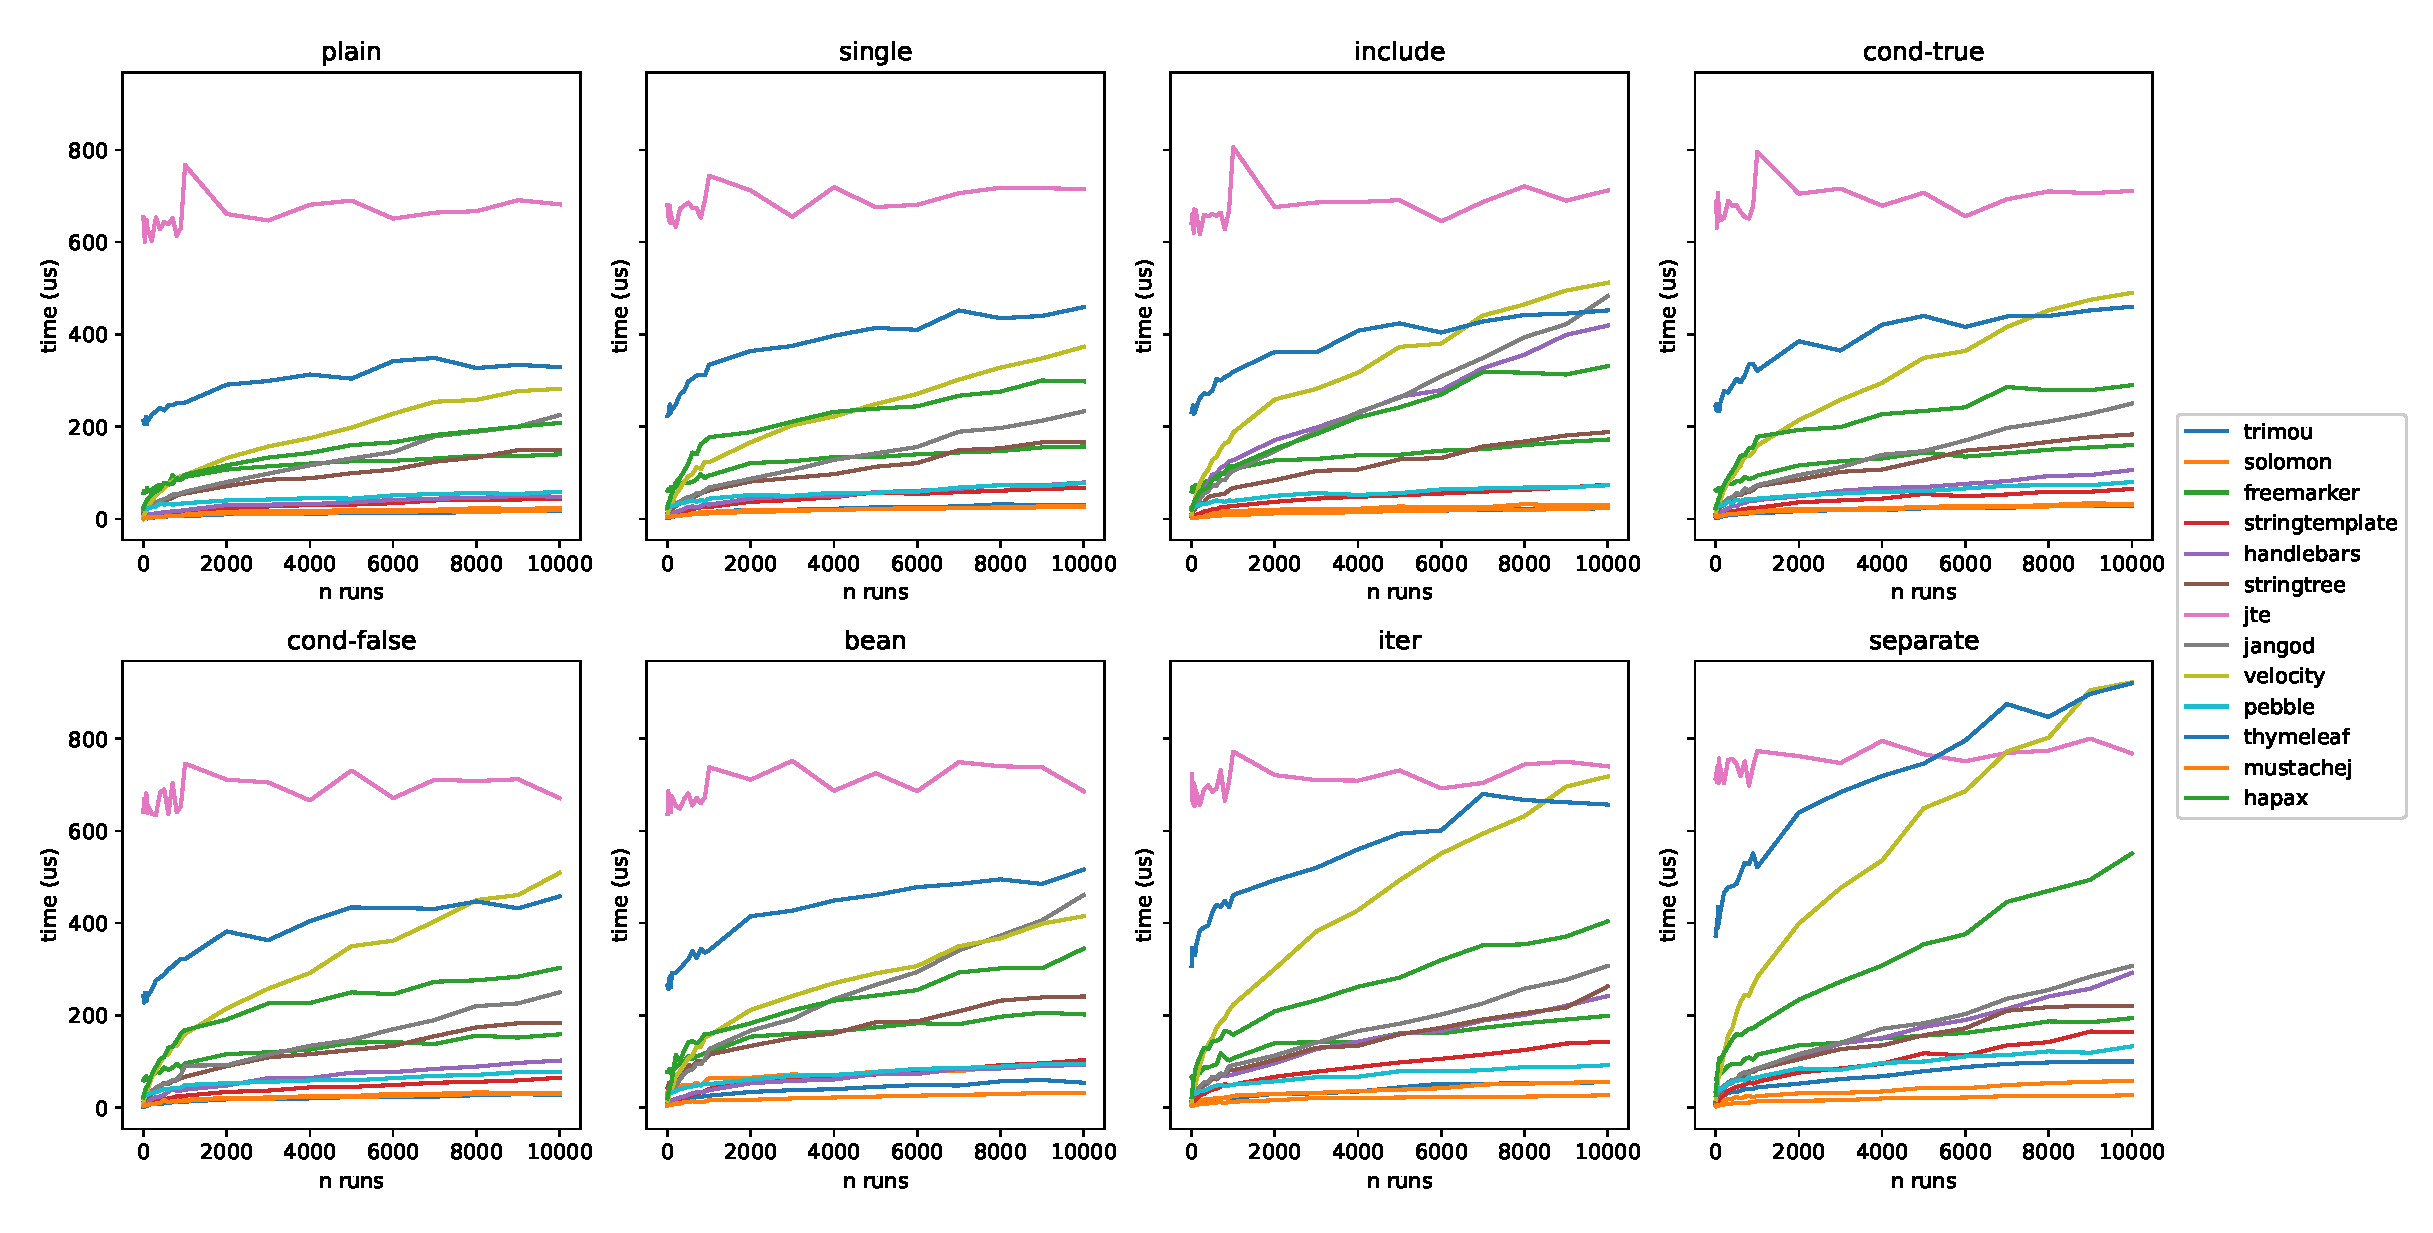
\includegraphics[width=\columnwidth]{Figures/graphs/wave4/2023-12-20avg.eps}
\caption{\label{results:wave4 pc}Performance Wave 4 Run on the Intel PC Platform}
\end{figure}

\subsection{Discussion}

There are several key points to take from the comparison of template engine performance on the two platforms.

All the performance measurements run roughly 10 times the speed on the Intel PC platform compared with the Raspberry Pi-based DUT platform. This, in itself, does not diminish the usefulness of the comparisons, however. neither of these platforms will be identical to current and future web platforms. For this research, the important aspect is the \emph{relative} performance of the different template engines in the different scenarios. The relative performance is indicated by the shapes of the curves and the points at which they cross.

The shapes of the curves in the two sets of measurements are broadly similar. For example, in both cases \emph{JTE} has a relatively high minimum duration and a relatively gentle slope, \emph{Velocity} has a much lower minimum duration but a steeper slope, and \emph{Thymeleaf} is somewhere in between those two. Where the two sets of measurements differ is in the crossing points. Consider the `separate' scenario, for example. On the PC platform, \emph{JTE} becomes a better choice than \emph{Thymeleaf} at around 5000 runs, and a better choice than \emph{Velocity} at around 7000 runs. On the DUT platform, however, \emph{JTE} becomes a better choice than \emph{Thymeleaf} at around 1000 runs, and a better choice than \emph{Velocity} at around 3000 runs. The slope of the graphs indicate that this difference will probably become increasingly important as the number of runs increases beyond 10,000. The effect of this can be seen in the energy comparison timings in \autoref{section:context energy}.  Further research is required to determine which specific differences between the two platforms cause these effects.

A minor, but encouraging, point is that there appears to be considerably less influence of `noise' on the performance measurements on the DUT platform. This is likely to be due in part by the longer time taken for the measurements but the relative simplicity of the operating system installation on the DUT device, with fewer background processes running, may also be a factor.

\section{The Feasibility of Comparing Component Energy Use}
\label{section:fse}

\subsection{Method}
\label{fse methodology}

The apparatus from \autoref{chapter:testrig} had already been used to compare the energy usage of web server software written in Java, so no extra support was needed to run the evaluation scenarios. However, the comparison apparatus had been designed to trigger execution of server code via requests from the \texttt{LOAD} device. To integrate the code from the performance study with this architecture required either changes to the performance study code, or the addition of a server to listen for trigger requests and invoke an appropriate performance study script.

For simplicity, and to minimise any accidental issues due to modification of the performance study code, it was decided to use one of the web servers compared during the evaluation of the apparatus and to invoke the performance study code using the \emph{Common gateway Interface} (CGI) protocol. CGI was designed as a method for invoking local programs from an HTTP request, so seemed a suitable choice for this task. The web server \emph{Lighttpd} had consumed the least energy when serving static pages when evaluated in \autoref{chapter:testrig} so this server was used.

Lighttpd is very configurable and was supplied with an example of the configuration needed to serve CGI requests. All that was required was to modify this configuration slightly: to indicate where to look for scripts to execute when a CGI request is received, and to add a mapping to indicate that shell scripts should be executed by the system shell \verb!/bin/bash!. The configuration changes were tested using a simple `hello world' CGI script.

Once the operation of the server had been confirmed, a CGI script was created which called the \emph{one.sh} script described in \autoref{chapter:performance}. This script evaluates a single template engine by running all the scenarios a specified number of times. For the initial experiments, a count of 1000 times for each scenario was used. As this was just an initial study to determine if any difference in energy consumption could be observed, each template engine was measured just once.

\subsection{Results}
\label{fse results}

The measured net energy use (after subtracting the `baseline' energy use of a quiescent system) for each of the template engines is shown in \autoref{fse:results:net 1000}.

\begin{table}[ht!]
\centering
\begin{tabular}{lccr}
\textbf{Engine} & \textbf{Energy (J)} \\
\hline
freemarker & 11.4936 \\
handlebars & 12.4403 \\
hapax & 10.7424 \\
jangod & 9.33103 \\
jte & 5.13393 \\
mustachej & 7.22679 \\
pebble & 8.48842 \\
solomon & 4.90431 \\
stringtemplate & 6.20053 \\
stringtree & 8.39519 \\
thymeleaf & 15.6721 \\
trimou & 7.98896 \\
velocity & 11.5069 \\
\end{tabular}
\caption{Average net energy use for 1000 sets of scenarios by template engine\label{fse:results:net 1000}}
\end{table}

\subsection{Discussion}
\label{fse discussion}

The results from \autoref{fse:results:net 1000} show a discernible difference in energy usage between the template engines. However, the scale of the difference is considerably less than shown in the performance figures from \autoref{chapter:performance}. Also, the energy use figures from this experiment do not align well with the performance figures. A striking example is \emph{JTE} which exhibited the slowest performance at 1000 repetitions of all the template engines in this cohort (see \autoref{multi:wave4-average}), yet shows the second lowest energy usage in this experiment.

While the energy usage figures from this experiment are interesting, they should not be considered authoritative for several reasons:

\paragraph{Low number of samples}
The typical duration of 1000 repetitions of the suite of template scenarios for these template engines was between 10 and 20 seconds. The experimental test apparatus was configured to sample current and voltage at 1 second intervals which meant that each run only had 10-20 readings from which to derive an average energy figure (see \autoref{fse2:energy single 1000}). The readings varied widely during this period, so it is entirely possible that one or two outliers, either high or low, could noticeably perturb the average.

\begin{figure}[htbp]
  \centering
  % \def\svgwidth{\columnwidth}
  \includesvg[width=\columnwidth]{Figures/graphs/Energy/SingleRun1000.svg}
  \caption{Energy Readings From 1,000 scenarios}
  \label{fse2:energy single 1000}
\end{figure}

\paragraph{System `noise' and other external factors}
The contribution to the energy due to the components in these experiments is small compared to the energy usage of the system as a whole. Background processes and the general functioning of the system add `noise' to the measurements which can, on occasion, overshadow the energy usage of the components. When combined with the low number of samples and the experiment being run only once for each template engine, this also acts to reduce confidence in the comparison.

\paragraph{Unrepresentative scenarios}
The performance experiments in \autoref{chapter:performance} were designed to investigate the differences in behaviour of template engines in specific circumstances. In those experiments it made sense to repeat each specific scenario many times in order to amplify the differences and minimise the influence of external factors. If the intention is to obtain a directly applicable comparison between the energy usage of components when deployed to real applications, then a more representative scenario might be more appropriate.

\paragraph{Platform differences}
The performance experiments in \autoref{chapter:performance} were conducted on an Intel CPU running a 64-bit operating system, while the energy experiments in this section were conducted on the energy measurement apparatus which uses an ARM CPU running a 32-bit operating system. Differences between the performance results for the two different platforms are explored in \autoref{section:perf dut}.

\subsection{Conclusions}
\label{fse conclusions}

The initial conclusions from this experiment were that there was an apparent difference in the energy consumption of the template engine components when tested with the simple scenarios used for the performance comparisons, but further investigation was required. Future experiments would need to include a larger number of cycles within each run and the averaging of several runs to minimise the impact of system noise and other external factors as well as the construction of further, more representative, scenarios.


\section{More Samples and Averaging}
\label{section:fse2}

Following the approach taken in \autoref{section:fs1} and \autoref{section:perf dut}, a further energy comparison experiment was carried out in which each template engine was exercised 10,000 times for each of the performance test scenarios. Both energy use and time taken to process the test scenario were recorded. Each set of 10,000 was repeated three times for each template engine and the results were averaged to reduce the effect of system noise and interference.

\subsection{Results}
\label{fse2 results}

Increasing the number of repetitions of each template scenario served to reduce the variability of the energy readings in most cases. \autoref{fse2:energy single 10000} shows relatively consistent energy use during the measurement, with the addition of noise in a similar manner to the performance graph in \autoref{results:fullsolomon}.

\begin{figure}[htbp]
  \centering
  % \def\svgwidth{\columnwidth}
  \includesvg[width=\columnwidth]{Figures/graphs/Energy/SingleRun10000.svg}
  \caption{Energy Readings From 10,000 runs of \emph{Pebble}}
  \label{fse2:energy single 10000}
\end{figure}

\subsubsection{Energy Use}
\label{fse2 results energy}

\autoref{fse2:energy graph} shows the comparative energy use of the selected template engines with the centre dot representing the average of three runs and the range bars indicating maximum and minimum values. The graph clearly shows a wide variation in energy use between template engines for this scenario.

\begin{figure}[htbp]
  \centering
  % \def\svgwidth{\columnwidth}
  \includesvg[width=\columnwidth]{Figures/graphs/Energy/ComponentEnergy.svg}
  \caption{Averaged Energy Use by Template Engine}
  \label{fse2:energy graph}
\end{figure}

\subsubsection{Time Taken}
\label{fse2 results time}

\autoref{fse2:time graph} shows the time taken for the experiments shown in \autoref{fse2:energy graph}. There is also a wide variation between these figures which has some similarity to the energy usage but also has some important differences. For example, \emph{Hapax} shows as faster than \emph{Jangod}, but achieves that speed at the expense of extra energy usage.

\begin{figure}[htbp]
  \centering
  % \def\svgwidth{\columnwidth}
  \includesvg[width=\columnwidth]{Figures/graphs/Energy/ComponentTime.svg}
  \caption{Averaged Test Duration by Template Engine}
  \label{fse2:time graph}
\end{figure}

\subsubsection{Running Power Consumption}
\label{fse2 results power}

Having recorded both total energy use and time taken for each of the test runs, it became possible to derive the average running power consumption for each of the template engines by dividing the total energy used by the total time taken for each run. These derived values are shown in \autoref{fse2:power graph}.

\begin{figure}[htbp]
  \centering
  % \def\svgwidth{\columnwidth}
  \includesvg[width=\columnwidth]{Figures/graphs/Energy/ComponentPower.svg}
  \caption{Averaged Running Power by Template Engine}
  \label{fse2:power graph}
\end{figure}

\subsection{Discussion}
\label{fse2 discussion}

Unlike the improved performance experiments in \autoref{section:fs2}, the experiments which provided the energy and duration values in this section only represented a single quantity of requests. However, there is a clear variation between the evaluated template engines in both time taken and energy used. 

While the emphasis of this research is on comparing the energy used by different software components, the addition of performance measurements also enables investigation into the running power consumption of the different components and its potential use as an indicator of the relationship between performance and energy use. This relationship between energy use and time taken, as shown in \autoref{fse2:power graph}, is also different for the different template engines. In these results, \emph{Hapax} uses approximately twice the running power of \emph{JTE}. A component which uses less running power is not necessarily a better or worse choice than one which uses more, however. The important values for capacity planning are performance, which can be used to determine the number of machines required to serve a desired number of requests per second, and total energy use, which indicates which components are more or less energy-efficient for the same task.

The disparity in calculated running power, even at a single quantity of repetitions, indicates that performance measurement is a poor analogue for energy use. However, the combination of the different measurements can help decide which components to choose, at least for this kind of scenario on this kind of platform. For example, in this experiment, \emph{Velocity} exhibits both the worst performance and the worst energy use so is unlikely to be a good choice.\emph{JTE}, on the other hand performs consistently well in both performance and energy use. One concern with \emph{JTE} in this scenario is that it completes so quickly that it does not allow enough time for a large number of energy readings.

\subsection{Conclusions}
\label{fse2 conclusions}

This experiment confirms that there is an observable difference in both performance and energy use of different template engine components. Combining the two sets of measurements also shows that the different components have different relationships between performance and energy use. This indicates that, without prior calibration specific to the code being executed, performance measurement is not a reliable way to predict overall energy use.

Results from \autoref{chapter:performance} showed that the different components perform differently under different volumes of requests, but the experiments in this section all used the same volume. It is expected that energy use, time taken, and running power will also vary depending on request volume.  Further experimentation is needed to validate this assumption as well as to determine how well such abstract test scenarios represent real deployments.

\section{Measuring Template Engines in Context}
\label{section:context energy}

\subsection{Introduction and Scope}
\label{cce intro}

The preceding experiments have concentrated on testing the behaviour of specific template engine features. While informative, such scenarios may not be fully representative of the way such template engines are used on the web. To better simulate that kind of usage an example web page was converted to an intermediate template using the \emph{GILT} template language discussed in \autoref{chapter:intermediate}. This intermediate template was then used to generate templates for a selection of template engines. The performance and energy usage of the selected template engines were compared using the apparatus described in \autoref{chapter:testrig}. The results of these comparisons are described in \autoref{cce results}.

\subsection{Methods}

\subsubsection{Selecting A Web Page and Generating Templates}
\label{cce pages}

Web pages on the public internet vary widely. From simple pages holding a single image or a small amount of text to large, sprawling pages containing many distinct sections and structures. For the purposes of this investigation, a page was needed containing representative usage of many of the template features compared in previous sections. Such a web page would need boilerplate text, simple substitutions, template inclusion, iteration through a list, and boolean selection. Method invocation is not supported across the full range of template engines, so that was excluded from this investigation.

The desired set of features are found on many blogs and other similarly-structured sites. The blog page used for the comparison between servers in \autoref{chapter:testrig} only contains the content for a single page with little opportunity for iteration, so it was decided to use the `front page' of a blog which contains multiple tags, archive links, and sections for different blog posts. To avoid potential repeatability issues with relying on an externally-controlled website, a snapshot of the front page of the website and blog associated with this research\footnote{\url{https://greenprogrammer.net/}} was selected.

\subsubsection{Generating Templates}
\label{cce gilt}

The aim of the experiment was to compare the performance and energy use of a range of template engines. In order to do this, templates would be needed in appropriate template languages for each of the engines. The intention was to generate these templates from a single intermediate template coded using the \emph{GILT} intermediate language described in \autoref{chapter:intermediate}. It quickly became clear during the creation of this intermediate template that the only way to test for correctness was to generate a template for one of the candidate template engines and then expand that template using the appropriate template engine. This process was cumbersome, and led to confusion whenever there was an error as to whether the issue was in the intermediate template, the template generation driver for the chosen target template language, or the behaviour of the target template language itself.

To eliminate some of these variables, and allow verification of the correctness of the intermediate template without using it to generate a template in a different template language, a new template engine was created. This template engine, named \emph{gilt-native}, uses the \emph{GILT} intermediate language directly as its template language. This template engine enabled faster development and testing of intermediate templates without the need for third-party template engines and direct comparison of the expanded template with the expected web page. 
% Updated results graphs from \autoref{chapter:fs2} including the new \emph{gilt-native} template engine are shown in \autoref{cce results}.

Once a intermediate template containing uses of all the desired features was complete, the \emph{GILT} template generator was used to generate appropriate templates for each of the template engines.

\subsubsection{Selecting a Test Method}
\label{cce method}

When evaluating the effectiveness of the test rig in \autoref{chapter:testrig}, web pages were served by a selection of servers using both dynamic (Wordpress) and static page data. When comparing performance and energy use of components in \autoref{section:fse} and \autoref{section:fse2}, each test scenario was invoked directly using a script. Both approaches showed clear differences between energy use but in the server-based tests the differences between server implementations had the potential to overshadow the differences between components. In order to directly compare the performance and energy use of the candidate template engines it was decided to run each engine from a script in a similar manner to the component tests.

Scripts from the separate scenario tests were copied and modified to load appropriate context data and invoke each template engine using its \verb!EngineDriver! implementation using its generated template.

\subsubsection{Evaluating the Template Engines}
\label{cce evaluation}

Prior to use on the measurement apparatus, each template engine was invoked with the intended context data and generated template, and the result was compared with the expected web page. This highlighted several problems which needed to be addressed before the performance and energy use of the template engines could be measured and compared.

The most common problems were differences in the handling of `whitespace' such as space, tab, and newline characters. All the template engines in this cohort were designed primarily to generate output formatted using HTML. The rendering of HTML by web browsers is mostly insensitive to the presence or absence of such whitespace, so the template engine developers have not always cared about exactly preserving whitespace when generating web pages. For example, \emph{velocity} failed to preserve a new line following a template inclusion directive (see \autoref{velocity diff}.

\begin{figure}[htbp]
  \centering
  \includegraphics[width=\columnwidth]{Figures/graphs/Page/velocity-diff.png}
  \caption{Difference in generated whitespace}
  \label{velocity diff}
\end{figure}

After examining the output from these template engines, the acceptance criteria for a successful template expansion were widened to allow such minor differences in whitespace.

Other template engines, however, had bigger issues. Even though each of the template engines considered for this phase of the investigation had passed the individual tests in \autoref{chapter:performance}, some failed to generate acceptable output for this more complex scenario. For example, \emph{Solomon}, which had performed flawlessly on the individual scenarios, initially generated a much smaller output file than the other template engines. When the output was examined it was clear that the template inclusion directives had failed. To understand why this was happening, the source code for the \emph{Solomon} template engine was used instead of the provided library, and instrumented to discover the cause of the problem. An issue was discovered in the filenames of the templates to be included. \emph{Solomon} expected the names of included templates to conform to the rules for identifier names in Java: starting with a letter then containing a combination of letters, digits, \verb!_! and \verb!$!. The filenames of the blog post summaries to be included had names beginning with their creation date in the form \verb!2022-10-23! which meant that the filenames were not valid Java identifiers. Once this issue was resolved, by renaming included template file to be valid Java identifiers, \emph{Solomon} generated the correct output. This issue was subsequently raised with the \emph{Solomon} developers, who relaxed this unnecessary restriction in a later release.

Of the remaining template engines, some initially  failed to process the generated template at all.

\emph{JTE}, which had performed well in the tests of individual features, uses an approach which converts a supplied template into Java source code, then compiles that source code and runs it to expand the template. This approach requires additional specialist annotation in templates to enable the correct Java code to be generated. Unlike all the other template engines, which provide access to data values via a shared context visible to all templates, \emph{JTE} requires that context value names and types be declared in a header section at the start of the template. When including one template in another, any context values used in the child template need to be both declared in the child template, and passed as `parameters' in the include directive. During the evaluation of individual template engine features and the development of the \emph{JTE} driver, no child template made use of context values, so this requirement was never discovered. Although the \emph{JTE} driver generated child templates with the correct declarations, it failed to generate the correct `parameters' in the parent template, which in turn meant that \emph{JTE} generated invalid Java code which \emph{JTE} could not compile. To add this feature to the \emph{JTE} driver would require the template generation code to model the complete, transitive, contents of every child template in order to generate a correct parent template. This would require major changes to the architecture of the template generator, so \emph{JTE} was excluded from this phase of the template engine evaluation.

\emph{Stringtemplate} also required included templates to be valid Java identifiers, but once this had been adjusted for \emph{Solomon} the template generation process still produced invalid templates. Further investigation determined that the \emph{Stringtemplate} driver was using incorrect delimiters for some situations. The driver was updated to correct this error, and then \emph{Stringtemplate} correctly processed the generated template.

\emph{Handlebars} crashed when attempting to expand the generated template. Investigation indicated that this was a problem with the specific version of the \emph{Handlebars} library which was being used which made some uses incompatible with recent versions of Java\footnote{\url{https://github.com/swagger-api/swagger-codegen/issues/10966}} \footnote{\url{https://teamtreehouse.com/community/broke-when-adding-blocks}}. Updating the library removed this problem, but revealed further issues. All previous comparisons had been performed with a single version of the \emph{Handlebars} library. Updating to a new version, even if the further issues could be addressed, would raise questions about the comparability of the measurements, so \emph{Handlebars} was also excluded from this phase of the template engine evaluation.

\emph{Mustachej} required some minor changes to the Driver, but otherwise functioned correctly.

\emph{Hapax} does not fully support loops and conditionals, so was excluded from this phase of the template engine evaluation.

\emph{Thymeleaf} employs an HTML-specific syntax which would require altering the intermediate template document in ways which would make it incompatible with the other template engines, so it was also excluded from this phase of the template engine evaluation.

Energy and performance comparisons were therefore performed on the following template engines:
\emph{trimou},
\emph{solomon},
\emph{freemarker},
\emph{stringtemplate},
\emph{stringtree},
\emph{jangod},
\emph{velocity},
\emph{pebble},
\emph{mustachej},
and \emph{gilt-native}.

A script was created to load a specified context and use a single template engine to expand the templates generated from the example website. Each page expansion was run 100,000 times. The overall run of 100,000 expansions was then repeated twice more, and the results averaged, to minimise the impact of external interference.

\subsection{Results}
\label{cce results}

The energy usage of the averaged runs for each template engine are shown in \autoref{cce:energy page 100000} and the time taken by each template engine is shown in \autoref{cce:time page 100000}. These two data sets have been combined to produce running power figures for each template engine, and these results are shown in \autoref{cce:power page 100000}

\begin{figure}[htbp]
  \centering
  % \def\svgwidth{\columnwidth}
  \includesvg[width=\columnwidth]{Figures/graphs/Page/Full-Page-Energy.svg}
  \caption{Energy Usage of 100,000 page expansions}
  \label{cce:energy page 100000}
\end{figure}

\begin{figure}[htbp]
  \centering
  % \def\svgwidth{\columnwidth}
  \includesvg[width=\columnwidth]{Figures/graphs/Page/Full-Page-Time.svg}
  \caption{Time taken for 100,000 page expansions}
  \label{cce:time page 100000}
\end{figure}

\begin{figure}[htbp]
  \centering
  % \def\svgwidth{\columnwidth}
  \includesvg[width=\columnwidth]{Figures/graphs/Page/Full-Page-Power.svg}
  \caption{Average Running Power for 100,000 page expansions}
  \label{cce:power page 100000}
\end{figure}

\subsection{Analysis}
\label{cce analysis}

In \autoref{cce:energy page 100000} there is an observable difference between the energy usage of the different template engines. There is also a clear distinction between two groups of template engines: those which use less than 100J, and the four template engines which consume over 350J for the same scenario. This distinction suggests that there is some key aspect of the design or implementation which differs between the two groups. Investigation of the reason or reasons for this difference is out of scope for this research, but such a large difference could indicate a potentially fruitful area of future research.

The times taken shown in \autoref{cce:time page 100000} largely echo the energy usage results, with the same four template engines taking the longest to process the specified number of template expansions. The relationship between the template engine energy usage and duration is not constant, however. For example, when considering only energy usage, \emph{velocity} is noticeably worse than \emph{stringtemplate}, but for time taken, these positions are reversed. This difference can be clearly seen in \autoref{cce:power page 100000}. \emph{velocity} uses more energy in a shorter time, which shows as a much higher running power consumption.

While the power figures in \autoref{cce:power page 100000} can be useful when comparing components whose energy usage and time taken are roughly similar, they are not indicative of any notion of efficiency. \emph{mustachej}, for example, shows by far the highest running power consumption, but is still among the lowest for total energy consumption and time taken to complete the task.

\section{Discussion}
\label{ce duscussion}

This chapter has explored some different ways of comparing the energy usage of template engine components. Comparing software components is challenging because, unlike full applications, they cannot be executed without other software to configure, initiate, execute, and shut down the components. This external software can potentially influence the time and energy performance of the components. The results in this chapter show that software components do not usually perform identically in different scenarios. 

The experiments have shown clear differences in energy usage between template engine components. The combined individual scenario experiments in \autoref{section:fse2} provide a ranking of template engines by energy usage as shown in the first data column of \autoref{ce rankings}. If considered in isolation, this ranking would seem to provide a way to select the most energy-efficient template engine for a project. However, when the same template engines were compared using the arguably more realistic scenario of generating a complete web page, the rankings were very different as shown in the second data column of \autoref{ce rankings}.

\begin{table}[ht!]
\centering
\begin{tabular}{lrr}
\multirow{2}{*}{Template Engine} 
      & \multicolumn{2}{c}{Energy Efficiency Ranking} \\
& Individual Scenarios & Full Page Generation \\
\hline
freemarker & 8 & 3 \\
gilt-native & - & 8 \\
handlebars & 9 & - \\
hapax & 11 & -\\
jangod & 10 & 6 \\
jte & 1 & - \\
mustachej & 2 & 5 \\
pebble & 6 & 2 \\
solomon & 3 & 1 \\
stringtemplate & 4 & 7 \\
stringtree & 7 & 10 \\
thymeleaf & 12 & - \\
trimou & 5 & 4 \\
velocity & 13 & 9 \\
\end{tabular}
\caption{Comparative energy-efficiency rankings for template engines\label{ce rankings}}
\end{table}

\subsection{Comparisons With the Performance Studies}
\label{ce performance}

The performance studies in \autoref{chapter:performance} could also potentially be used to rank the template engine components based solely on performance. However, these experiments revealed that the various template engines exhibit different performance characteristics based on the overall volume of requests. Any potential rankings based on the performance studies of individual template engine features would only be valid for the specific features being evaluated at that particular request volume. The energy comparisons were performed at fixed request volumes in order to gain a workable number of energy usage samples, but it is expected that energy-efficiency of some template engines would also vary with request volume.

\subsection{The Relationship Between Energy Use and Performance}
\label{ce relationship}

For the components evaluated in this chapter, the relationship between energy usage and time taken was neither constant between template engines nor constant between scenarios. This relationship, formulated as average running power is shown in \autoref{fse2 results power} and \autoref{cce:power page 100000}. In both scenarios the ratio between energy use and time taken, expressed as Joules per second (Watts) ranged from under 0.3 W to around 0.6 W. This variability suggests that models which aim to predict energy usage based on time performance are unlikely to be generally applicable.

\section{Conclusions}
\label{ce conclusions}

The key conclusion drawn from the experiments in this chapter is that different software components can vary widely in both energy usage and performance when performing the same task, and that the relationship between performance and energy usage is not constant across different evaluation scenarios. The implication of this is that models which attempt to predict energy use solely from other measurements such as performance, task complexity, or static analysis of code will not yield generally-applicable results.
% \chapter{Conclusions}
\label{chapter:conclusions}

\section{Reflection}

This research has explored ways to improve the sustainability, particularly as regards reducing energy consumption and its associated greenhouse gas emissions, of large-scale software systems. Such systems are created and maintained by software developers, so an investigation was carried out into how software developers learn their skills. This study concluded that, despite an increased interest in sustainability among students and guidance from accreditation bodies, UK Higher Education computing courses do not generally appear to include education on improving the sustainability of computing technology. Where teaching of sustainability topics is included, it is mostly about personal and institutional sustainability rather than preparing students to tackle big sustainability issues in their future careers. Other paths into computing careers are more varied and difficult to evaluate, but little evidence of the inclusion of sustainability was found there either.

In the absence of broad training in the development of sustainable software, an approach was explored of improving the energy usage of existing systems by substituting software components with ones which use less energy to do the same job. A feasibility study was conducted which showed that within one category of software components, performance varied by up to thousands of times. Further component performance comparisons were conducted which indicated that individual component performance varies depending on the task and the load. Selecting components with better performance for a particular application could potentially reduce the number of computers needed to run a popular service, thereby reducing both energy usage in operation and the embodied carbon costs of manufacturing and disposal of the hardware.

While optimising performance can help reduce hardware requirements, it is not a direct measurement of energy use. A prototype test apparatus was designed and constructed to support automated, programmable comparison of the energy used by applications or software components under different scenarios and loads. Comparisons using the apparatus produced some interesting results, including that the popular \emph{WordPress} application which is used by a very large number of websites requires a lot more energy to serve each web page than a traditional `static' website.

Substitution of components as a strategy is only feasible if the cost and complexity of replacing one component with another is low. However, software components provide different APIs and are rarely directly interchangeable. To explore potential solutions to this problem, a framework was constructed to simplify the creation of `drivers' for different component APIs. Components can also differ in data formats and data storage requirements. To explore this issue, an intermediate data format and associated conversion tools were created to simplify the generation of appropriate data for each component. This combination of framework, data format, and tools was then used to create more complex scenarios to evaluate the energy consumption of the components compared for performance earlier. The results showed that while in some cases the components which performed fastest also used the least energy, this was not always the case.

The implication of this research is that while improving software performance can help improve sustainability, it is not a good proxy for operational energy usage. A more effective and direct way to assess and reduce the energy usage of a software system is to use an energy comparison apparatus to integrate energy comparison both while evaluating and selecting components and as part of an automated \emph{Continuous Integration} process to track energy usage changes between versions of software.

\section{Evaluation of Research Objectives}

A set of research objectives were described in \autoref{section:research objectives}. This section examines the outcomes and evaluates the effectiveness of this research against these objectives.

\subsection{Explore how software developers learn their skills and the inclusion of sustainability}

This objective was addressed in two phases.

In the first phase, academic literature and public data from the computing industry on the background of software developers were explored in order to direct the next phase of the research in this area. The conclusion of this phase was that although there are many routes into a career in software development, the most popular route is via Higher Education (HE) such as a university or college. However, there was little information about the inclusion of sustainability in this data. 

In the second phase, a study was designed to investigate the inclusion of sustainability topics in UK HE computing courses. The study was intended to examine public course information from all UK universities which offer computing degree courses, but it quickly became apparent that UK universities do not typically provide information in enough detail to determine if their computing courses include coverage of sustainability. The study was extended to request information from course staff about the inclusion of sustainability in their courses. A relatively low proportion of course staff responded to the request, but most respondents replied that there was little or no coverage of sustainability in their computing courses. Further research was then conducted to examine the websites of the same cohort of universities to look for sustainability-related policies. While almost all the universities had some form of sustainability policy in place, most of those were limited to personal or institutional sustainability rather than equipping students to improve the sustainability of their future careers.

This research was partially effective in determining the inclusion of sustainability in the training and education of software developers. Information was hard to obtain, but that which was obtained indicated a general lack of inclusion of sustainability education in software developers' education. However, the relatively small sample of responses reduces confidence in the conclusions.

\subsection{Explore the differences in performance of example software components}

This objective was addressed in three phases.

In the first phase, a representative category of software component was selected and a small cohort of implementations was chosen from within that category. A software performance test harness was created and used to evaluate the performance of the implementations in a range of scenarios. This initial feasibility study clearly indicated a large performance difference between these components. However, there were some issues with the interaction between the performance test harness and the components being evaluated.

In a second phase, an improved performance test harness was constructed to address the issues raised by the feasibility test. This confirmed the large differences in component performance found in the feasibility study and also discovered that component performance varies not only between components and scenarios but also between the volume of requests.

In a third phase, the improved performance tests were executed on a different computing platform. the results of this experiment largely confirmed the results from the second phase, but with some discrepancies.

This research was effective in uncovering the scale and complexity of the performance differences between supposedly-equivalent software components. This stands in sharp contrast to the documentation and other public information available about these components. Such documentation rarely mentions performance, and when it does it is usually in vague terms such as `fast' or `powerful'. Using this information to select components with optimum performance for a desired application could potentially reduce the number of computers needed to serve that application, thus reducing the embodied carbon in the system.

\subsection{Compare the energy use of software during operation}

This objective was addressed in three phases.

In the first phase, an apparatus was designed, constructed and evaluated to assess the energy usage of running software under different scenarios. This phase of the research was very successful and the resulting apparatus was then used for energy comparisons in the following two phases.

In a second phase, the energy comparison apparatus was used to compare the energy usage of a selection of popular web server applications, both when serving static and dynamic web pages. The results of this comparison clearly showed not only a difference in energy usage between servers but also highlighted the large hidden energy cost of dynamic website generation.

In a third phase, the cohort of software components which had been compared for performance were then compared for energy use. Energy use was compared both when re-running the performance evaluation scenarios and when running new scenarios designed to be more representative of common use. The results of this comparison showed differences in the energy usage of the components but the relationship between performance and energy usage was different for each of the components.

This research was effective in showing that an apparatus could be constructed to compare the energy usage of both components and whole applications in a variety of scenarios. Importantly, this apparatus was built for much less cost than traditional lab equipment and provided software interfaces so it could be included in the `continuous integration' processes commonly used to test software during development. Comparisons run on the apparatus revealed the wide range of differences in energy consumption between equivalent software, in particular the much larger energy required to serve websites using WordPress software.

The ability to compare both performance and energy usage of the same software also highlighted the differences in the relationship between the two metrics. Although many attempts have been made in the literature to derive ways of using performance to predict energy usage, this research clearly showed that the relationship between the two varies both between components and between usage scenarios. Any models which claim to relate the two metrics will therefore only be of use in very limited circumstances.

\subsection{Explore substitution of incompatible components using drivers and template generation}

This objective was addressed in two phases.

In the first phase, a driver framework was created to allow independent loading of template engine components into a comparison framework. A new component could be added and compared by writing a driver for the new component with no need to modify or recompile the comparison framework. The comparison framework was used for comparing both component performance and component energy usage.

In a second phase, an intermediate language was designed to represent common features of template languages and a software tool was constructed to convert templates expressed in the intermediate language into the various formats required by different template engines. The template generation tool also used a driver mechanism, allowing new template languages to be added without the need to modify the generation tool. This intermediate language and tool were successfully used to generate representative web pages for template engine comparison, based on a real website, for each of the supported template engines.

This research was effective in showing that there are ways to simplify the complex and potentially expensive task of comparing software components. The development of standard tools for performance and energy usage comparison as well as tools to overcome the differences in component APIs and data formats has helped compare the performance and energy-use differences between components. With the ability to compare components comes the ability to select ones with better performance and lower energy use. This, in turn, could lead to an overall reduction in energy use and associated carbon emissions.

\subsection{Research Objectives Conclusions}

Of the four research objectives, three were very successful, providing a range of contributions to knowledge which should help improve the sustainability of software systems. The objective to explore the inclusion of sustainability in the education of software developers was less successful due to the small amount of available information on which to base conclusions. However, that research did provide the justification for exploring ways to improve the sustainability of software systems through other means which do not require rapid changes to the structure and content of Higher Education.

\section{Contributions To Knowledge}
\label{section:contributions}

This research has generated several contributions to knowledge, which are described below.

\subsection{The State of Sustainable Computing Teaching in UK HE}
\label{contrib:HE}

When considering media attention, the requirements of accrediting bodies, and institution publicity, it is easy to assume that Higher Education computing courses are preparing the next generation of software developers and other decision makers to address the ongoing climate emergency and the huge contribution of computing systems to greenhouse gas emissions.

This research has shown that, in the UK at least, this is not yet the case. Courses claim accreditation based on older standards which do not include sustainability clauses, and those institutions which do include sustainability teaching tend to favour personal and institutional sustainability advice such as campus waste recycling programs and remembering to switch off room lighting. Even where teaching staff are aware of bigger issues, it has often proved difficult to fit computing system sustainability topics into an already crowded curriculum.

\subsection{A Novel Self-Contained Apparatus for Comparing Software Performance and Energy Consumption}
\label{contrib:apparatus}

While there have been several studies which have measured or compared the energy usage of software, they typically involve expensive laboratory equipment or manual measurements, only work with specific computer hardware, or concentrate on the investigation of theoretical models rather than enabling energy measurement and comparison as part of routine software development and testing.

This research has developed a self-contained, low-cost prototype for an apparatus which can be integrated into the automated `continuous integration' processes used by many industry teams when developing and testing software. The apparatus can operate without human intervention to compare performance and energy use of a wide range of software applications and software components  with customisable scenarios and load levels. The apparatus is designed to integrate with automated test systems but also offers a manual web interface which can be useful when evaluating candidate software to include in a project.

\subsection{Energy Use and Performance Comparisons for a Cohort of Web Server Implementations}
\label{contrib:servers}

The apparatus described in \autoref{chapter:testrig} was evaluated by comparing the energy use and performance of a variety of web server implementations, including two of the most commonly used servers worldwide, to serve some representative web content. The results clearly indicate the differences between the implementations. This information is not available elsewhere.

\subsection{The Relative Energy Usage of WordPress Compared to Static Websites}
\label{contrib:wordpress}

\emph{WordPress} is a very popular tool for creating, managing, and serving websites, yet users are mostly unaware of its energy consumption. This research has shown that \emph{WordPress} requires many times more energy to serve the same web pages compared with a traditional `static' website.

\subsection{A Novel Extendable Java Framework for Template Engine Comparison}
\label{contrib:framework}

Selecting a template engine component for a project can be a daunting task. The lack of detailed information provided by the component creators leads to a choice between committing to one component and hoping it is a good choice, or conducting comparative experiments. Constructing rigorous comparative experiments can be complex, but that complexity can be reduced using the template engine comparison software framework constructed for this research. When using this framework all that is needed is to define the template scenarios to be tested and write driver implementations to suit the API of each candidate template engine. The framework takes care of dynamically loading the correct drivers and templates, running the selected scenarios, and collecting results ready for analysis.

\subsection{A Novel Intermediate Language and Generation Tools for Templated Systems}
\label{contrib:gilt}

Template engines do not just differ in APIs, but also in the markup and syntax used for the templates. Constructing correct templates for an unfamiliar template engine can be both challenging and laborious. Keeping multiple templates in sync with each other as the collection of comparison scenarios and candidate template engines changes or grows can seem like an impossible task. The GILT intermediate language and associated tools assist in generating compatible templates for multiple template engines from a single definition. Adding support for a new template engine requires the writing of a single driver. Addition or modification of a template requires addition or modification of a single GILT template and re-running the template generator.

\subsection{Energy Use and Performance Comparisons for a Cohort of Template Engine Implementations}
\label{contrib:engines}

As part of this research, the comparison framework described in \autoref{chapter:performance}, the intermediate language described in \autoref{chapter:intermediate}, and the apparatus described in \autoref{chapter:testrig} were utilised to compare the energy usage and performance of a cohort of open source template engines of the kind commonly used for the generation of dynamic web pages. These comparisons involved multiple platforms and a range of scenarios and load levels. This information is not available elsewhere.

\subsection{A Challenge to the Notion of Execution Speed as a Proxy for Software Energy Usage}
\label{contrib:speed as proxy}

It seems to be a common opinion, even being referred to as `folklore' in one paper, that energy usage of software is in some way related to the time taken to accomplish a task. Many researchers have attempted to construct models to relate the two quantities, in the hope that relatively simple and cheap performance measurements could be used to produce an estimate of energy usage.

This research has shown that when evaluating a range of software which does a broadly similar task, there is no constant or reliable relationship between execution speed and energy use. Different components have different relationships which vary between different evaluation scenarios. This research leads to the conclusion that the only practical and effective way to compare the energy use of software in operation is to measure it.

\subsection{A Challenge to the Notion of Task Complexity as a Proxy for Software Energy Usage}
\label{contrib:complexity as proxy}

A lot of writing on the topic of software energy usage has made the implicit or explicit assumption that the energy use of a software system is primarily dependent on the complexity of the task the software system performs. This may be true in cases where there is a very large difference in task complexity, and reducing task complexity as a strategy is likely to reduce overall energy usage. However, this research has shown that the architecture and design of the software to perform the task can also make a big difference, even when the task being performed is the same.

\subsection{The Efficacy of Component Substitution as a Strategy to Improve Software Sustainability}
\label{contrib:efficacy}

This research has discovered major differences in the performance and energy use of different software components when performing similar tasks. This clearly indicates that the choice of software components, either by component selection when designing a new system, or by component substitution in an existing system, could be a viable strategy to improve the sustainability of software 

\section{Future Work}
\label{section:future work}

Each of the studies in this research has also revealed the potential for further work.

\subsection{How Developers Learn}

While the results of the study on the sustainability content of UK HE computing courses were clear, it was concerning that there was so little public information available about the content of courses and modules. There is the potential to build on this study by investigating course content in more detail and attempting to discover the reasons or justification for why institutions typically make it so difficult both for potential students and for researchers and other interested parties to find out exactly what material is covered. Similarly, there is potential for further work exploring the technology, design and content choices which have led to the generally poor usability and reliability of university websites for such research.

Further research is also possible into the routes into careers in software development. The Stack Overflow Developer Survey \citep{StackOverflow2022} was useful in indicating the large proportion of software developers with a university qualification but stopped short of exploring the particular courses and course content. Such broad instruments provide no real indication of whether working software developers have ever received any education in sustainability. Further investigation, perhaps by surveying or interviewing a more targeted group of software developers might reveal other, potentially more effective, ways of equipping software developers with the understanding and skills needed to address large-scale sustainability problems.

Developer education is only one contributor to improving the sustainability of software. Further research is also needed into how developers and other decision-makers decide what software to make, how to make it, and how to evaluate whether it is suitable for its purpose. Such research could provide vital information on how best to promote information, processes, and tools which could help in developing more sustainable software systems.

\subsection{The Performance of Software Components}

The performance of software components under real conditions is an under-researched area. Historically, academic research has concentrated on the study of algorithms and data structures, but such abstract concepts are less-often considered in practical software development. Instead, software architects and developers attempt to design and construct systems from components but lack detailed information to use when selecting between many candidate components. Although a poor proxy for energy use in general, component performance comparisons can assist in designing software systems which require fewer or less powerful computer hardware systems to support them.

Within the category of template engines, further research is needed to investigate the design and characteristics of the selected components to investigate why their performance is so different, and if any software development or evaluation guidelines can be derived from this information.

This research has concentrated on one specific type of component, but there are a very broad range of software component types available, many of which also have a large number of substitution candidates. Further research is needed on the performance of other types of software component to investigate whether the results from this research are in any way representative.

Further research would also be useful into the impact on application performance of including multiple components and the possibility of models which would be able to predict or estimate overall performance or hardware requirements from a `software bill of materials'.

Most research in this area is limited by a lack of information, so there is also a potential for future research into ways to grow the range, detail and reliability of information available on software components. One approach to this might be to develop tools and and benchmarks which can be used to compare components. For template engine components these might take the form of standardised template scenarios which can be applied to many candidate template engines.

\subsection{An Apparatus To Compare Energy Usage}

The energy comparison apparatus developed in this study was only a prototype and thus there is ample opportunity for further research and development. Potential research areas include:

\begin{itemize}
    \item evaluating the use of alternative `DUT' platforms to better simulate the hardware used in commercial applications.
    \item evaluating or developing different energy-measurement circuitry which can deal with larger voltages and currents.
    \item improving the software to support multiple scenarios in a single test run.
    \item improving the software and database to support parallel operation of more than one apparatus.
    \item evolving the apparatus into a robust, self-contained device.
    \item integrating the apparatus with existing software `continuous integration' processes.
    \item enhancing the output and presentation of comparison results to better inform decision-making
\end{itemize}

Further research is also needed in the broader field of software energy usage measurement and communication. The results of energy usage of different software applications and components need to be disseminated so that potential users can make an informed choice without always needing to run their own energy usage comparisons. This in turn would need standards and repeatable methodologies as well as devices such as this apparatus.

\subsection{Substitution of Incompatible Software Components}

The GILT template language described in this dissertation is an initial version only. It has several shortcomings and potential improvements, as discussed in \autoref{comp:int language plus}, and there are many possibilities for further research in this area.

The software developed as part of this research to support substitution of components which are partly functionally equivalent but provide different APIs and data formats was specific to template engine components, but the approach is potentially applicable to other classes of component. Further research would be required to determine how broadly applicable this approach is to other contexts.

\subsection{The Energy Use of Software Components}

The performance results from evaluating the template engine components on the comparison apparatus are interesting, but do not align well with the performance results from the studies in \autoref{chapter:performance}. It was expected that the measured values would be different from the earlier experiments, as they were executed on different computers with different processors. What was not expected, however, was that the performance \emph{rankings} would be so different. There is clearly something else different about the two platforms, which needs further investigation.

The difference in performance rankings raises questions about the accuracy of the energy use comparisons and rankings for the same scenarios. These too need to be investigated, ideally at a range of different request volumes as was done for the performance studies in \autoref{section:fs2}. 

\subsection{Other Related Future Research}

This research has continually shown that there is a lack of detailed and reliable information about software in general, but about software components in particular. Electrical appliances have energy ratings, electronic components have data sheets, but software components mostly have little more than feature lists and usage instructions at best. Further research is needed into ways to obtain, share, and compare information about the characteristics of software components.

The server energy use comparisons in \autoref{chapter:testrig} highlighted the poor performance of dynamic websites and in particular, \emph{WordPress}. Further research is needed into the development of software which can make management of static websites as easy and flexible as \emph{WordPress} but without the high energy cost.



\clearpage
\addcontentsline{toc}{chapter}{References}
\pagestyle{plain}
\renewcommand\bibname{References}
\raggedright
\printbibliography

\label{glossary}
\printglossaries 

\newglossaryentry{ICT}{
    name=ICT,
    description={Information and Communication Technology, a collective term for the electronic and computer systems which enable the \gls{internet} and the \gls{web} as well as stand-alone computerised devices and the \gls{internet of things}}
}

\newglossaryentry{sustainability}{
    name=sustainability,
    description={The ability of something to endure. Used in this dissertation to refer to the specific sustainability of human life and our supportive ecosystems on Earth}
}

\newglossaryentry{un goals}{
    name=UN Sustainable Development Goals,
    description={A set of 17 `goals' aimed at improving the \gls{sustainability} of humanity and the environment}
}

\newglossaryentry{sustainability ledger}{
    name=sustainability ledger,
    description={A metaphorical `balance sheet' of forces and actions which improve and/or worsen global \gls{sustainability}}
}

\newglossaryentry{sustainable computing}{
    name=sustainable computing,
    description={One of the names given to the intersection of the disciplines of \gls{sustainability} and \gls{computing}}
}

\newglossaryentry{computing sustainability}{
    name=computing sustainability,
    description={One of the names given to the intersection of the disciplines of \gls{sustainability} and \gls{computing}}
}

\newglossaryentry{computing and sustainability}{
    name=computing and sustainability,
    description={One of the names given to the intersection of the disciplines of \gls{sustainability} and \gls{computing}}
}

\newglossaryentry{green computing}{
    name=green computing,
    description={One of the names given to the intersection of the disciplines of \gls{sustainability} and \gls{computing}}
}

\newglossaryentry{distributed system}{
    name=distributed system,
    description={A computer system comprising more than one separate software or hardware node which communicate over a network}
}

\newglossaryentry{client}{
    name=client,
    description={A role in a \gls{distributed system} which sends network requests or messages to a \gls{server}}
}

\newglossaryentry{server}{
    name=server,
    description={A role in a \gls{distributed system} which receives and responds to network requests or messages from a \gls{client}}
}

\newglossaryentry{client-server}{
    name=client-server,
    description={A \gls{distributed system} in which computing elements have one of two roles: \gls{client} or \gls{server}}
}

\newglossaryentry{internet}{
    name=internet,
    description={A massive \gls{distributed system} which enables a wide range of services including email, social media, digital telephony, and the \gls{web}}
}

\newglossaryentry{web}{
    name=World-Wide Web,
    description={A distributed information system enabled by the \gls{internet} and accessed using a \gls{web browser}}
}

\newglossaryentry{web browser}{
    name=web browser,
    description={Software which enables users to access (also known as \emph{browse} or \emph{surf}) the information available on the \gls{web}}
}

\newglossaryentry{internet of things}{
    name=internet of things,
    description={The addition of sensors and other non-interactive devices to the internet to gather, interpret and transfer information as well as operate internet-connected equipment}
}

\newglossaryentry{the cloud}{
    name=the cloud,
    description={An abstraction model which treats multiple processing and data storage systems, typically located in large \gls{datacenter}s, as a single bank of assignable resources}
}

\newglossaryentry{cloud computing}{
    name=cloud computing,
    description={Any software and data systems which use resources in \gls{the cloud}}
}

\newglossaryentry{datacenter}{
    name=datacenter,
    description={A single building or collection of buildings providing shared support for a large amount of computing resources}
}

\newglossaryentry{dark web}{
    name=dark web,
    description={Information and services which are accessed using web technology but not listed in search data or linked from public pages. This makes such information largely invisible to general web users}
}

\newglossaryentry{intranet}{
    name=intranet,
    description={A section of the \gls{web} protected behind a login or other security approach and therefore inaccessible to external web browsers}
}

\newglossaryentry{client-side processing}{
    name=client-side processing,
    description={Code which executes on a \gls{client} device, rather than requiring a request to a \gls{server}}
}

\newglossaryentry{server-side processing}{
    name=server-side processing,
    description={Code which executes on a \gls{server}, typically in response to a request or message from a \gls{client} device}
}

\newglossaryentry{http}{
    name=HTTP,
    description={Hypertext Transfer Protocol, the basic protocol used to transfer requests ans responses between web browsers and web servers}
}

\newglossaryentry{https}{
    name=HTTPS,
    description={Hypertext Transfer Protocol Secure, an extension of the \gls{http} protocol in which requests and responses are encrypted}
}

\newglossaryentry{global warming}{
    name=global warming,
    description={Also known as 'climate change'. An observed increase in global average temperature over time}
}

\newglossaryentry{PUE}{
    name=power usage effectiveness,
    description={(PUE) An indication of the proportion of consumed energy used above that needed for the desired work}
}

\newglossaryentry{greenhouse gases}{
    name=greenhouse gases,
    description={A range of gases, including carbon dioxide and methane, which contribute to the \gls{greenhouse effect} when released into the atmosphere}
}

\newglossaryentry{greenhouse effect}{
    name=greenhouse effect,
    description={A process in which infra-red radiation is reflected back to a planet surface by the composition of the atmosphere rather than escaping into space. This capturing of heat energy leads to an overall increase in temperature}
}

\newglossaryentry{programming language}{
    name=programming language,
    description={A language used to instruct computing devices on what to do and how to do it. programming languages are usually textual but may also be graphical (e.g. Scratch\footnote{\url{https://scratch.mit.edu/}}) or symbolic (e.g. APL \citep{Falkoff1978})}
}

\newglossaryentry{web application}{
    name=web application,
    description={A software application which makes use of the \gls{web}. Web applications are typically distributed systems making use of one or more servers as well as web browsers}
}

\newglossaryentry{artificial intelligence}{
    name=artificial intelligence,
    description={The application of software and data systems to process information and reason in a manner based on living intelligence. Machine learning based on neural networks is an approach to achieve artificial intelligence}
}

\newglossaryentry{zombie}{
    name=zombie,
    description={In this context a zombie is a slang term for a computer system or application which continues operation even though it is no longer used by humans or other computer systems}
}

\newglossaryentry{upgrading}{
    name=upgrading,
    description={A strategy for improving the performance or operating costs of a computer system by replacing computing hardware with newer, more efficient, components}
}

\newglossaryentry{consolidating}{
    name=consolidating,
    description={A strategy for improving the operating costs of a computer system by sharing computing hardware between multiple systems}
}

\newglossaryentry{virtualisation}{
    name=virtualisation,
    description={A strategy for consolidating computer systems by running multiple \gls{virtual machine}s under the control of a \gls{hypervisor}}
}

\newglossaryentry{virtual machine}{
    name=virtual machine,
    description={An installation of an \gls{operating system} and applications running alongside other virtual machines under the control of a \gls{hypervisor}}
}

\newglossaryentry{hypervisor}{
    name=hypervisor,
    description={A form of \gls{operating system} which acts to manage access to the \gls{bare metal} of a computing system from multiple \gls{virtual machine}s}
}

\newglossaryentry{operating system}{
    name=operating system,
    description={A software system which provides services to applications, isolating them from the specifics of the underlying computing hardware. Current common operating systems include Windows, MacOS, and Linux}
}

\newglossaryentry{containerisation}{
    name=containerisation,
    description={An alternative to \gls{virtualisation} in which multiple isolated software systems can share aspects of a single underlying operating system. Containerised applications are typically smaller than virtualised applications because they do not need to duplicate existing operating system features}
}

\newglossaryentry{embedded system}{
    name=embedded system,
    description={A software system is described as `embedded' when it is tied to, and often developed alongside, specific computer hardware. Embedded systems often run on \gls{bare metal} without the need for an \gls{operating system}, or with a custom or \gls{real time} operating system}
}

\newglossaryentry{real time}{
    name=real time,
    description={A term used to describe software optimised for immediate response to events and stimuli. Common operating systems such as Windows or Linux are not classed as `real time' as they use process scheduling algorithms which can cause delays or interruptions to application software}
}

\newglossaryentry{bare metal}{
    name=bare metal,
    description={A term used when software runs on real rather than \gls{virtualised} computer hardware. In \gls{embedded system}s, the term `bare metal' is also used when software runs without the need for an \gls{operating system}}
}

\newglossaryentry{virtualised}{
    name=virtualised,
    description={A term used when a computer system executes in a \gls{virtual machine} rather than on \gls{bare metal} hardware}
}

\newglossaryentry{dynamic scaling}{
    name=dynamic scaling,
    description={The process of automatically starting up and shutting down virtual servers or application containers to meet increases or decreases in demand}
}

\newglossaryentry{template engine}{
    name=template engine,
    description={Also sometimes known as a \emph{template processor}, \emph{templating engine}, or \emph{templater}, this is a software application or library which combines a generic \gls{template} with dynamic data to create a composite output document}
}

\newglossaryentry{template language}{
    name=template language,
    description={The symbols, grammar and linguistic elements which are allowable in a \gls{template} for a particular \gls{template engine}. Typically a template language specifies the syntax for \gls{boilerplate} and \gls{placeholder}s within the template document}
}

\newglossaryentry{template processor}{
    name=template processor,
    description={Another name for a \gls{template engine}. For consistency, this thesis always uses the term \gls{template engine}}
}

\newglossaryentry{template}{
    name=template,
    description={A specification of an output document consisting of \gls{boilerplate} text and \gls{placeholder}s}
}

\newglossaryentry{boilerplate}{
    name=boilerplate,
    description={Blocks of predefined text in a \gls{template} which are included as-is in the output document when the template is rendered by a \gls{template engine}}
}

\newglossaryentry{placeholder}{
    name=placeholder,
    description={An indication in a \gls{template} of where, and potentially how, to include data provided when the template is rendered by a \gls{template engine}}
}

\newglossaryentry{computing}{
    name=computing,
    description={The term used by \citet{Denning1989} to include all aspects of the specification, architecture, design, construction, evaluation, maintenance, and management of solutions and products which use computer technology}
}

\newglossaryentry{software engineering}{
    name=software engineering,
    description={A field within \gls{computing} which applies engineering principles and computer programming expertise to develop, test, and maintain software applications}
}

\newglossaryentry{computer systems engineering}{
    name=computer systems engineering,
    description={A field within \gls{computing} which applies engineering principles and computer programming expertise to develop, test, and maintain computer systems}
}

\newglossaryentry{software development}{
    name=software development,
    description={A field within \gls{computing} which includes conceiving a goal, evaluating feasibility, analysing requirements, design, implementation, testing and release management}
}

\newglossaryentry{informatics}{
    name=informatics,
    description={A field within \gls{computing} concerned with representation and transformation of information}
}

\newglossaryentry{data science}{
    name=data science,
    description={A field within \gls{computing} concerned with representation, storage and manipulation of data}
}

\newglossaryentry{information science}{
    name=information science,
    description={A field within \gls{computing} concerned with analysis, collection, classification, manipulation, storage, retrieval, movement, dissemination, and protection of information}
}

\newglossaryentry{computer science}{
    name=computer science,
    description={A field within \gls{computing} which includes both theoretical disciplines such as algorithms, theory of computation, and information theory, and applied disciplines such as the design and implementation of hardware and software}
}

\newglossaryentry{performance}{
    name=performance,
    description={In \gls{computing}, performance is usually used to refer to speed. In software, performance relates to the speed of the software in performing a given task. In hardware, performance is usually related to the speed at which the hardware can operate. Performance is inversely related to the time taken to perform a task}
}

\newglossaryentry{speed}{
    name=speed,
    description={In \gls{computing}, speed is often used interchangeably with performance. Speed is conceptually easy to measure for tasks that have a defined start and end - a faster task completes in less time. Speed is less easy to measure for services or applications that run until manually stopped}
}

\newglossaryentry{efficiency}{
    name=efficiency,
    description={In \gls{computing}, efficiency is commonly used in the sense that an efficient system is one which achieves an objective using minimal resources. The resources in question may include such things as time, energy, disk space, computer memory or any other scarce or costly resource. Where a specific resource is considered, the term can add a modifier, for example energy-efficiency or memory-efficiency}
}

\newglossaryentry{energy use}{
    name=energy use,
    description={A measure of the amount of energy used to achieve an objective. In \gls{computing}, energy use typically refers to the amount of electrical energy required for specific computing hardware to run software to complete the aims of the software. See also \gls{power consumption}}
}

\newglossaryentry{power consumption}{
    name=power consumption,
    description={A measure of the amount of energy used to achieve an objective. In \gls{computing}, power consumption typically refers to the amount of power required at any time for specific computing hardware to operate a long-running software system. See also \gls{energy use}}
}

\newglossaryentry{side-effects}{
    name=side-effects,
    description={In a template language, a side-effect is anything which happens as a result of a template placeholder expression other than the production of text for the output document. Examples might be modifying the operation of other placeholder expressions, controlling the operation of the template engine as a whole, or executing code on the underlying computer system}
}

\newglossaryentry{functional requirements}{
    name=functional requirements,
    description={Requirements that a system must meet in order to be considered fit for purpose. Functional requirements can usually be phrased in a way which allows for a yes/no or pass/fail answer}
}

\newglossaryentry{non-functional requirements}{
    name=non-functional requirements,
    description={Aims that a system should meet in order to be considered fit for purpose. Non-functional requirements are often vague or aspirational and can be difficult to measure}
}

\newglossaryentry{soft requirements}{
    name=soft requirements,
    description={An alternative name for \gls{non-functional requirements}.}
}

\newglossaryentry{design pattern}{
    name=design pattern,
    description={An description of a common software design approach. Eaxh design pattern is phrased in terms of four elements: the pattern name, the problem it addresses, the solution it provides, and the consequences of adopting that solution \citep{Gamma1994}}
}

\newglossaryentry{strategy design pattern}{
    name=strategy pattern,
    description={A software \gls{design pattern} in which alternate implementations of a solution can be treated interchangeably by sharing a common abstraction}
}

\newglossaryentry{lazy evaluation}{
    name=lazy evaluation,
    description={A software technique in which calculation or processing of derived values is deferred until the values are used. The main advantage of this approach is that derived values never need to be calculated if they are never used. This can be particularly significant if a calculation involves a relatively slow process such as requesting information from a remote system. The opposite approach to lazy evaluation is \gls{eager evaluation}}
}

\newglossaryentry{eager evaluation}{
    name=eager evaluation,
    description={A software technique in which calculation or processing of derived values is performed as soon as the input values are available. The main advantage of this approach is that derived values are already available when required, which can improve the responsiveness of a software application. The opposite approach to eager evaluation is \gls{lazy evaluation}}
}

\newglossaryentry{continuous integration}{
    name=continuous integration,
    description={A software technique in which software consisting of multiple collaborating parts is assembled and tested by an automated process. This process is performed whenever any of the component parts of the system are changed, to ensure that changes to individual parts do not affect the behaviour or performance of the larger system}
}

\newglossaryentry{embedded}{
    name=embedded,
    description={A software system is described as `embedded' when it is designed for a specific hardware configuration. Often the hardware and software for an embedded system are designed together}
}

\newglossaryentry{cross-compile}{
    name=cross-compile,
    description={Cross-compilation is a software development technique involving creating software on one machine, typically one set up as a development workstation, and using software tools to generate code which will run on a different device. Cross-compilation is commonly done when developing software for \gls{embedded} systems}
}

\newglossaryentry{JavaBeans}{
    name=JavaBeans,
    description={A feature of the Java \gls{programming language} that allows some object methods to be accessed as if they are fields. To be accessible as a JavaBean, a class must have a zero-argument constructor and methods with specific name patterns. See \url{https://docs.oracle.com/javase/8/docs/technotes/guides/beans/index.html}}
}

\newglossaryentry{classpath}{
    name=classpath,
    description={A classpath is an path-style environment variable containing a sequence of places for the Java Virtual Machine to look for class files when loading an application. The entries in the classpath may be directories in a file system, individual class files, or \emph{JAR} archive files}
}

\newglossaryentry{black box}{
    name=black box,
    description={A black box component is one which is used in whole and without the ability to modify the way it works. Black box component reuse is a process in which a component is reused without modification}
}

\newglossaryentry{white box}{
    name=white box,
    description={A white box component is one which is provided in the form of source code which may be modified or used in part. White box component reuse is a process in which a component is used as a source of code for modification.}
}


\captionsetup[figure]{list=no}
\captionsetup[table]{list=no}
\captionsetup[lstlisting]{list=no}
% \addtocontents{toc}{\setcounter{tocdepth}{0}}
\appendix
\begin{appendices}
\renewcommand\chaptername{Appendix}

\raggedbottom

\chapter{Java Template Engines on GitHub}
\label{appendix:engines}

\begin{singlespace}
\begin{itemize}
\item httl \verb!https://github.com/httl/httl!
\item Rocker \verb!https://github.com/fizzed/rocker!
\item Trimou \verb!https://github.com/trimou/trimou! \verb!http://trimou.org/!
\item jte \verb!https://github.com/casid/jte!
\item Liqp \verb!https://github.com/bkiers/Liqp!
\item Chunk \verb!https://github.com/tomj74/chunk-templates!
\item Smarty4J \verb!https://github.com/linux-china/smarty4j!
\item Rhythm \verb!https://github.com/rythmengine/rythmengine!
\item Water \verb!https://github.com/tiagobento/watertemplate-engine!
\item Wit \verb!https://github.com/febit/wit!
\item Basis \verb!https://github.com/badlogic/basis-template!
\item japid \verb!https://github.com/branaway/Japid!
\item japid42 \verb!https://github.com/branaway/japid42!
\item gt-engine \verb!https://github.com/mbknor/gt-engine!
\item gt-engine-play2 \verb!https://github.com/mbknor/gt-engine-play2!
\item Cambridge \verb!https://github.com/erdincyilmazel/Cambridge!
\item golang-like \verb!https://github.com/proninyaroslav/java-template-engine!
\item Min Velocity \verb!https://github.com/pfmiles/min-velocity!
\item Mixer2 \verb!https://github.com/nabedge/mixer2!
\item Panettone \verb!https://github.com/caelum/vraptor-panettone!
\item Carrot \verb!https://github.com/codeka/carrot!
\item PowerStat \verb!https://github.com/PowerStat/TemplateEngine!
\item Knotx \verb!https://github.com/Knotx/knotx-template-engine!
\item Inflectible \verb!https://github.com/gvlasov/inflectible!
\item te4j \verb!https://github.com/whilein/te4j!
\item static-mustache \verb!https://github.com/sviperll/static-mustache!
\item vtte \verb!https://github.com/hgschmie/vtte!
\item jade \verb!https://github.com/dhanji/jade!
\item Soulspace \verb!https://github.com/lsolbach/TemplateEngine!
\item jtt \verb!https://github.com/tokuhirom/jtt!
\item sitebuilder \verb!https://github.com/JonathanGiles/sitebuilder!
\item succinct \verb!https://github.com/tliron/succinct!
\item jelly \verb!https://github.com/pranitbose/jelly!
\item jjenkov \verb!https://github.com/jjenkov/template-engine!
\item antlr-template \verb!https://github.com/worstenemy/antlr-template!
\item datatree-templates \verb!https://github.com/berkesa/datatree-templates!
\item Simple-Template \verb!https://github.com/jalian-systems/Simple-Template!
\item Template72 \verb!https://github.com/template72/template72!
\item stencil \verb!https://github.com/impossibl/stencil!
\item coffeemaker \verb!https://github.com/mouse0w0/coffeemaker!
\item Cedilla \verb!https://github.com/ansorre/Cedilla!
\item rstl \verb!https://github.com/rstl/rstl!
\item templar \verb!https://github.com/synapticloop/templar!
\item jhaml \verb!https://github.com/iafonov/jhaml!
\item ljincheng \verb!https://github.com/ljincheng/template!
\item disc99 \verb!https://github.com/disc99/template!
\item iNamik \verb!https://github.com/iNamik/iNamik-Template-Engine!
\item Mini-templator \verb!https://github.com/bsorrentino/minitemplator!
\item Jakotem \verb!https://github.com/moznion/jakotem!
\item swiftmarker \verb!https://github.com/swiftech/swiftmarker!
\item stuartdd \verb!https://github.com/stuartdd/template!
\item zazl \verb!https://github.com/zazl/zazl!
\item josson \verb!https://github.com/octomix/josson!
\item luther94 \verb!https://github.com/luther94/templateEngine!
\item Yan \verb!https://github.com/GmailYan/TemplateEngine!
\item Holdbelief \verb!https://github.com/holdbelief/TemplateEngine!
\item buckhx \verb!https://github.com/buckhx/TemplateEngine!
\item kettlescott \verb!https://github.com/kettlescott/TemplateEngine!
\item grub \verb!https://github.com/prezi/grub!
\item twig4j \verb!https://github.com/palmenhq/twig4j-core!
\item ngoy \verb!https://github.com/krizzdewizz/ngoy!
\item templet \verb!https://github.com/toluju/templet!
\item moennig \verb!https://github.com/rnoennig/template-engine!
\item tempera \verb!https://github.com/kasonyang/tempera!
\item antiaction \verb!https://github.com/antiaction/common-template-engine!
\item templates4j \verb!https://github.com/danishdynamite/templates4j!
\item LagoVista \verb!https://github.com/LagoVistaTechLLC/java-template!
\item maddaluno \verb!https://github.com/danielemaddaluno/simple-template-engine!
\item Debuggable \verb!https://github.com/gaelyk/debuggable-template-engine!
\item Shitstorm \verb!https://github.com/hectorlf/shitstorm-template-engine!
\item Poorman \verb!https://github.com/chtz/PoormanTemplateEngine!
\item Toy \verb!https://github.com/CHZone/toy_template_engine!
\item Tiny \verb!https://github.com/ferronrsmith/tiny-template-engine-java!
\item Albirar \verb!https://github.com/albirar/albirar-template-engine!
\item Quarkus \verb!https://github.com/DavutKeskin/Quarkus-Template-Engine!
\item Tinwatchman \verb!https://github.com/tinwatchman/Simple-Java-Template-Engine!
\item Atian \verb!https://github.com/ate47/AtianTemplateEngine!
\item adrianromero \verb!https://github.com/adrianromero/templateengine!
\item mentjes \verb!https://github.com/rnentjes/Very-simple-templates!
\item round-string \verb!https://github.com/round-lang/round-string!
\item templait \verb!https://github.com/seanrmilligan/templait!
\item trodix \verb!https://github.com/trodix/teengine!
\item nate \verb!https://github.com/SeanTAllen/nate!
\item engender \verb!https://github.com/kazimsarikaya/engender!
\item ccte \verb!https://github.com/CCLooMi/ccte!
\item yyuc \verb!https://github.com/yyuc/StringTemplate!
\item hte \verb!https://github.com/HBTGmbH/hte!
\item gastirit \verb!https://github.com/gastirit/templateengine!
\item jst \verb!https://github.com/hibnico/jst!
\item Rocheteau \verb!https://github.com/JeromeRocheteau/templater!
\item quick-termplates \verb!https://github.com/rajeshputta1983/quick-templates!
\item TEFT \verb!https://github.com/marggx/TEFT!
\item stencil \verb!https://github.com/erichonorez/stencil!
\item simple-mustache \verb!https://github.com/piotrkot/simple-mustache!
\item jetg \verb!https://github.com/fbsgen/jetg!
\item yatte \verb!https://github.com/glefur/yatte!
\item simple-templates \verb!https://github.com/sbohmann/simple-templates-java!
\item Nabucco \verb!https://github.com/NABUCCO/org.nabucco.framework.template!
\item kala \verb!https://github.com/Glavo/kala-template!
\item scalpel \verb!https://github.com/bluetorch/scalpel!
\item JTemplate \verb!https://github.com/And390/JTemplate!
\item utl \verb!https://github.com/lamerexter/utl!
\item temporize \verb!https://github.com/h34tnet/temporize!
\item Webengine \verb!https://github.com/ASofterSpace/WebEngine!
\item fronton \verb!https://github.com/skozlov/fronton!
\item Rtpl \verb!https://github.com/shenfe/Rtpl!
\item raptor \verb!https://github.com/jebl01/raptor!
\item djtemplate4j \verb!https://github.com/tanob/djtemplate4j!
\item contemplate \verb!https://github.com/almondtools/comtemplate!
\item templ8 \verb!https://github.com/mpobrien/templ8!
\item jangular \verb!https://github.com/cupmanager/jangular!
\item Hotplate \verb!https://github.com/terazzo/Hotplate!
\item Trensetim \verb!https://github.com/trensetim/java-template!
\item jaml \verb!https://github.com/zhuochun/jaml!
\item jagglate \verb!https://github.com/nobuoka/Jagglate!
\item Simplate \verb!https://github.com/SuperPagh/Simplate-engine!
\item Jango \verb!https://github.com/CptPhenomeno/Jango!
\item BenFaerber \verb!https://github.com/benfaerber/WebServer!
\item libjlte \verb!https://github.com/ergor/libjlte!
\item JTTemplate \verb!https://github.com/chen3961/JTTemplate!
\item minitemplator \verb!https://github.com/chdh/minitemplator-java!
\item omnitemplate \verb!https://github.com/omnifaces/omnitemplate!
\item temmental \verb!https://github.com/jfgiraud/temmental!
\item mistigri \verb!https://github.com/jido/mistigri-java!
\item lostTemple \verb!https://github.com/Darkylin/lostTemple!
\item KDom \verb!https://github.com/Kademi/KDom!
\item Templatefeather \verb!https://github.com/aliteralmind/templatefeather!
\item Javamarkup \verb!https://github.com/kmmanoj/JavaMarkup!
\item cupjate \verb!https://github.com/marvinsiq/cupjate!
\item java-latte \verb!https://github.com/peterhalada/java-latte!
\item jBraces \verb!https://github.com/anars/jBraces!
\item Jinjava \verb!https://github.com/HubSpot/jinjava!
\end{itemize}
\end{singlespace}
\chapter{Source code referenced in the text}
\label{appendix:sourcecode}

\verbatimfont{\footnotesize}

\section*{Test code for the Template Engines in the Feasibility Study}
\label{appendix:smoketest}

Example `Smoke Test' to check that the \emph{TemplateSystem} implementation for a specific template engine compiles and expands a template. Note that this test does not check that the resulting document is fully correct, only that it generates a document containing appropriate context data without errors or crashes.

\begin{verbatim}
package test;

import java.util.Arrays;
import org.junit.jupiter.api.Test;
import wrapper.TemplateSystem;
import wrapper.ThymeleafTemplateSystem;

class SingleEngineSmokeTest {
  @Test
  void test() {
    TemplateSystem system = new ThymeleafTemplateSystem();
    system.defineTemplate("smoke", 
        "[[# th:each=\"person: *{family}\"] [[${person}]] [/]]");
    system.putContext("family", Arrays.asList(new String[] { "Frank", "Margaret" }));
    CheckResult result = system.check("smoke", 1, "hello Frank", "smoke");
    System.out.println(result);
  }
}
\end{verbatim}

\section*{Test Code for the Template Engine Plugin}
\label{appendix:plugintest}

Example `Smoke Test' to check that the \emph{TemplateSystem} implementation for a specific template engine compiles and expands a template. Note that this test does not check that the resulting document is fully correct, only that it generates a document containing appropriate context data without errors or crashes.

\begin{verbatim}
package test;

import java.util.Arrays;
import org.junit.jupiter.api.Test;
import wrapper.TemplateSystem;
import wrapper.ThymeleafTemplateSystem;

class SingleEngineSmokeTest {
  @Test
  void test() {
    TemplateSystem system = new ThymeleafTemplateSystem();
    system.defineTemplate("smoke", 
        "[[# th:each=\"person: *{family}\"] [[${person}]] [/]]");
    system.putContext("family", Arrays.asList(new String[] { "Frank", "Margaret" }));
    CheckResult result = system.check("smoke", 1, "hello Frank", "smoke");
    System.out.println(result);
  }
}
\end{verbatim}

\section*{Template Engine Plugin Driver}
\label{appendix:driver}

\verb!init()! requires no parameters but is slightly unusual in that it returns an object of type \verb!TemplateEngine!. In most cases this method simply returns the same \verb!TemplateEngine! object that it was called on, but this approach supports \gls{template engine}s with more complex initialisation requirements which might need to create a new or different \verb!TemplateEngine! object. As a beneficial side-effect, this approach also allows for a `fluent' style of method calling \citep{JavaDesignPatterns} as shown in \autoref{code:fluent}.

\begin{lstlisting}[backgroundcolor=\color{black!5},escapeinside={(*}{*)},tabsize=2,label={code:fluent},caption={Fluent method call},captionpos=b]
    Context context = new MapContext();
    engine.init().expand(context, "example");
\end{lstlisting}

\verb!expand()! requires the context and the name of the template as parameters, and returns a text string containing the resulting document. The definition of the \verb!TemplateEngine! interface is shown in \autoref{code:TemplateEngine.java}.

\begin{lstlisting}[backgroundcolor=\color{black!5},escapeinside={(*}{*)},tabsize=2,label={code:TemplateEngine.java},caption={TemplateEngine interface},captionpos=b]
package shared;
import java.io.IOException;
import com.efsol.context.Context;

public interface TemplateEngine {
    TemplateEngine init() throws IOException;
    String expand(Context context, String template) throws IOException;
}\end{lstlisting}

\section*{Plugin Driver Factory}
\label{appendix:driverfactory}

The Java \verb!interface! definition for these classes contains just two methods, as shown in \autoref{code:EngineFactory.java}.

\begin{lstlisting}[backgroundcolor=\color{black!5},escapeinside={(*}{*)},tabsize=2,label={code:EngineFactory.java},caption={EngineFactory interface},captionpos=b]
package shared;

import java.io.File;
import java.io.IOException;

public interface EngineFactory {
    TemplateEngine create(File templateFolder) throws IOException;
    String getName();
}
\end{lstlisting}

Each plugin contains a class named \verb!plugin.EngineFactory! which implements this interface.  As an example, the code for this class in the \emph{Trimou} plugin is shown in \autoref{code:trimou:EngineFactory.java}.

\begin{lstlisting}[backgroundcolor=\color{black!5},escapeinside={(*}{*)},tabsize=2,label={code:trimou:EngineFactory.java},caption={Trimou EngineFactoy class},captionpos=b]
package plugin;

import java.io.File;
import java.io.IOException;
import shared.TemplateEngine;

public class EngineFactory implements shared.EngineFactory {
    @Override
    public TemplateEngine create(File templateFolder) throws IOException {
        return new TrimouTemplateEngine(templateFolder).init();
    }

    @Override
    public String getName() {
        return "trimou";
    }
}
\end{lstlisting}

\section*{Performance Test Runner}
\label{appendix:testrunner}

\begin{lstlisting}[backgroundcolor=\color{black!5},escapeinside={(*}{*)},tabsize=2,label={code:Run.main},caption={Run class main method},captionpos=b]
public static void main(String[] args) {
    List<String> real = new ArrayList<>();
    for (String arg : args) {
        if (arg.startsWith("-")) {
            if ("-v".equals(arg)) {
                Run.verbose = true;
            } else if ("-w".equals(arg)) {
                Run.warmup = true;
            }
        } else {
            real.add(arg);
        }
    }

    int nargs = real.size();
    String engineName = nargs > 0 ? real.get(0) : "dummy";
    String scenario = nargs > 1 ? real.get(1) : "plain";
    int n = nargs > 2 ? Integer.valueOf(real.get(2)) : 1;

    try {
        Run run = new Run(engineName, scenario, n);
        String stamp = format.format(new Date());
        CheckResult result = run.execute();
        if (verbose && result.status() != CheckStatus.OK) {
            System.err.println(result.engine() + "/" + result.test() + "\n  actual " + result.actual()
                + "\nexpected " + result.expected());
        }
        System.out.println(stamp + "," + result.engine() + "," + result.test() + "," + result.runs() + ","
            + result.time() + "," + result.status());
    } catch (Exception e) {
        System.err.println("ERROR engine:" + engineName + " scenario:" + scenario);
        e.printStackTrace();
    }
}
\end{lstlisting}

Within the \verb!try!..\verb!catch! block, after processing the command-line arguments, the test runner calls the constructor method of the \verb!Run! class to create a new object, passing in the \gls{template engine} name, scenario name, and the number of times to expand the template. The constructor method stores the parameters for later use, applies the \verb!EngineFactory! technique described above to load and initialise the specified \gls{template engine} driver, and creates a \verb!StopWatch! object to measure the time taken to run the specified number of template expansions. The code for the Run constructor method is shown in \autoref{code:Run.Run}.

\begin{lstlisting}[backgroundcolor=\color{black!5},escapeinside={(*}{*)},tabsize=2,label={code:Run.Run},caption={Run class constructor method},captionpos=b]
public Run(String engineName, String scenario, int n) throws IOException {
    this.engineName = engineName;
    this.scenario = scenario;
    this.n = n;

    this.engine = new EngineFactory().create(new File("../" + engineName + "/templates/test/"));
    this.clock = new StopWatch();
}
\end{lstlisting}

Once the \verb!Run! object is constructed, the \verb!execute! method is called to run the experiment. This method returns a \verb!CheckResult! object which contains a tuple of (\gls{template engine}, scenario, number of expansions, time taken, and test status). The test status is determined by whether the result of expanding the template matches the expected result. This result is then emitted as a CSV row which can be appended to a data file for later processing. The code for the \verb!execute! method is shown in \autoref{code:Run.execute}.

\begin{lstlisting}[backgroundcolor=\color{black!5},escapeinside={(*}{*)},tabsize=2,label={code:Run.execute},caption={Run class execute method},captionpos=b]
private CheckResult execute() throws IOException {
    TestSpec test = loadTest();
    Tract page = test.getPage();
    String templateName = test.getTemplateName();

    // do one run before starting the clock, to separate one-time costs from ongoing ones
    if (warmup) {
        engine.expand(page, templateName);
    }
    clock.reset();
    for (int i = 0; i < n - 1; ++i) {
        engine.expand(page, templateName);
    }
    String result = engine.expand(page, templateName);
    clock.stop();

    return new CheckResult(engineName, scenario, n, clock.get(),
        test.getExpected().equals(result) ? CheckStatus.OK : CheckStatus.NOTMATCHED,
        test.getExpected(), result);
}
\end{lstlisting}

\section*{Performance Test Scripts}
\label{appendix:testscripts}

\subsection*{Script \texttt{run.sh}}
\label{appendix:run.sh}

\begin{lstlisting}[backgroundcolor=\color{black!5},escapeinside={(*}{*)},tabsize=2,label={code:run.sh},caption={Script `run.sh'},captionpos=b]
#!/bin/bash
engine="${1:-dummy}"
shift
scenario="${1:-plain}"
shift
n="${1:-1}"
shift
#echo run engine=${engine} scenario=${scenario} n=${n} "$@"
java -classpath "../${engine}/bin:../${engine}/lib"'/*:../shared/bin:bin' runner.Run ${engine} ${scenario} ${n} "$@"
\end{lstlisting}

\subsection*{Script \texttt{one.sh}}
\label{appendix:one.sh}

\begin{lstlisting}[backgroundcolor=\color{black!5},escapeinside={(*}{*)},tabsize=2,label={code:one.sh},caption={Script `one.sh'},captionpos=b]
#!/bin/bash
here="$(dirname "$(realpath "$0")")"
engine="${1:-dummy}"
shift
n="${1:-1}"
shift
#echo run engine=${engine} scenario=${scenario} n=${n} "$@"
for scenario in `ls scenarios`
do
  ${here}/run.sh ${engine} ${scenario} ${n} "$@"
done
\end{lstlisting}

\subsection*{Script \texttt{all.sh}}
\label{appendix:all.sh}

\begin{lstlisting}[backgroundcolor=\color{black!5},escapeinside={(*}{*)},tabsize=2,label={code:all.sh},caption={Script `all.sh'},captionpos=b]
#!/bin/bash
here="$(dirname "$(realpath "$0")")"
n="${1:-1}"
shift
for engine in `find .. -name 'EngineFactory.java' | awk 'FS="/" { print $2 }'`
do
if [ ! -f "../${engine}/SKIP" ]
then
  ${here}/one.sh ${engine} ${n} "$@"
fi
done
\end{lstlisting}

\subsection*{Script \texttt{fulldata.sh} Wave 1}
\label{appendix:fulldata1.sh}

\begin{lstlisting}[backgroundcolor=\color{black!5},escapeinside={(*}{*)},tabsize=2,label={code:fulldata1.sh},caption={Script `fulldata1.sh'},captionpos=b]
#!/bin/bash
here="$(dirname "$(realpath "$0")")"
echo stamp,engine,scenario,n,time,status
for (( n=1; n <= 10000; n += 1 ))
do
 ${here}/all.sh ${n} "$@"
done
\end{lstlisting}

\subsection*{Script \texttt{fulldata.sh} Wave 2}
\label{appendix:fulldata2.sh}

\begin{lstlisting}[backgroundcolor=\color{black!5},escapeinside={(*}{*)},tabsize=2,label={code:fulldata2.sh},caption={Script `fulldata2.sh'},captionpos=b]
#!/bin/bash
here="$(dirname "$(realpath "$0")")"
echo stamp,engine,scenario,n,time,status
${here}/all.sh 1 "$@"
${here}/all.sh 10 "$@"
${here}/all.sh 100 "$@"
${here}/all.sh 1000 "$@"
${here}/all.sh 10000 "$@"
\end{lstlisting}

\subsection*{Script \texttt{fulldata.sh} Wave 3}
\label{appendix:fulldata3.sh}

\begin{lstlisting}[backgroundcolor=\color{black!5},escapeinside={(*}{*)},tabsize=2,label={code:fulldata3.sh},caption={Script `fulldata3.sh'},captionpos=b]
#!/bin/bash
here="$(dirname "$(realpath "$0")")"
echo stamp,engine,scenario,n,time,status
${here}/all.sh 1 "$@"
${here}/all.sh 10 "$@"
${here}/all.sh 20 "$@"
${here}/all.sh 30 "$@"
${here}/all.sh 40 "$@"
${here}/all.sh 50 "$@"
${here}/all.sh 60 "$@"
${here}/all.sh 70 "$@"
${here}/all.sh 80 "$@"
${here}/all.sh 90 "$@"

for (( n=100; n <= 10000; n += 100 ))
do
 ${here}/all.sh ${n} "$@"
done
\end{lstlisting}

\subsection*{Script \texttt{fulldata.sh} Wave 4}
\label{appendix:fulldata4.sh}

\begin{lstlisting}[backgroundcolor=\color{black!5},escapeinside={(*}{*)},tabsize=2,label={code:fulldata4.sh},caption={Script `fulldata4.sh'},captionpos=b]
#!/bin/bash
here="$(dirname "$(realpath "$0")")"
echo stamp,engine,scenario,n,time,status
${here}/all.sh 1 "$@"
${here}/all.sh 10 "$@"
${here}/all.sh 20 "$@"
${here}/all.sh 30 "$@"
${here}/all.sh 40 "$@"
${here}/all.sh 50 "$@"
${here}/all.sh 60 "$@"
${here}/all.sh 70 "$@"
${here}/all.sh 80 "$@"
${here}/all.sh 90 "$@"

${here}/all.sh 100 "$@"
${here}/all.sh 200 "$@"
${here}/all.sh 300 "$@"
${here}/all.sh 400 "$@"
${here}/all.sh 500 "$@"
${here}/all.sh 600 "$@"
${here}/all.sh 700 "$@"
${here}/all.sh 800 "$@"
${here}/all.sh 900 "$@"

${here}/all.sh 1000 "$@"
${here}/all.sh 2000 "$@"
${here}/all.sh 3000 "$@"
${here}/all.sh 4000 "$@"
${here}/all.sh 5000 "$@"
${here}/all.sh 6000 "$@"
${here}/all.sh 7000 "$@"
${here}/all.sh 8000 "$@"
${here}/all.sh 9000 "$@"

${here}/all.sh 10000 "$@"
\end{lstlisting}

\subsection*{Script \texttt{fulldata.sh} Modified for \emph{Solomon}}
\label{appendix:fullsolomon.sh}

\begin{lstlisting}[backgroundcolor=\color{black!5},escapeinside={(*}{*)},tabsize=2,label={code:fullsolomon.sh},caption={Modified `fulldata1.sh'},captionpos=b]
#!/bin/bash
here="$(dirname "$(realpath "$0")")"
echo stamp,engine,scenario,n,time,status
for (( n=1; n <= 10000; n += 1 ))
do
 ${here}/one.sh 'solomon' ${n} "$@"
done
\end{lstlisting}

\section*{Code Improvements}

\subsection*{Original \emph{Hapax} Driver}
\label{appendix:hapax:driver1}

\begin{lstlisting}[backgroundcolor=\color{black!5},escapeinside={(*}{*)},tabsize=2,label={comp:hapax:driver1},caption={Original \emph{Hapax} Context Loop},captionpos=b]
for (String key : ContextUtils.iterable(context)) {
    Object value = context.getObject(key);
    putContext(key, value);
}
\end{lstlisting}

\subsection*{Improved \emph{Hapax} Driver}
\label{appendix:hapax:driver2}

\begin{lstlisting}[backgroundcolor=\color{black!5},escapeinside={(*}{*)},tabsize=2,label={comp:hapax:driver2},caption={Updated \emph{Hapax} Context Loop},captionpos=b]
        dict = TemplateDictionary.create();
        for (String key : ContextUtils.iterable(context)) {
            Object value = context.getObject(key);
            putContext(key, value);
        }
\end{lstlisting}

\subsection*{Original \emph{Stringtemplate} Driver}
\label{appendix:stringtemplate:driver1}

\begin{lstlisting}[backgroundcolor=\color{black!5},escapeinside={(*}{*)},tabsize=2,label={comp:stringtemplate:driver1},caption={Original \emph{Stringtemplate} expand method},captionpos=b]
public String expand(Context context, String templateName) {
    String template = templates.get(templateName);
    ST engine = new ST(template);
    for (String key : ContextUtils.iterable(context)) {
        Object value = context.getObject(key);
        engine.add(key, value);
    }
    return engine.render();
}
\end{lstlisting}

\subsection*{Improved \emph{Stringtemplate} Driver}
\label{appendix:stringtemplate:driver2}

\begin{lstlisting}[backgroundcolor=\color{black!5},escapeinside={(*}{*)},tabsize=2,label={comp:stringtemplate:driver2},caption={Updated \emph{Stringtemplate} expand method},captionpos=b]
public String expand(Context context, String templateName) throws IOException {
    StringTemplate template = group.getInstanceOf(templateName);
    for (String key : ContextUtils.iterable(context)) {
        Object value = context.getObject(key);
        template.setAttribute(key, value);
    }
    return template.toString();
}
\end{lstlisting}

\chapter{Template engine information sources}
\label{appendix:sources}

\url{https://en.wikipedia.org/wiki/Comparison_of_web_template_engines}
\url{https://handwiki.org/wiki/Comparison_of_web_template_engines}
\url{https://mvnrepository.com/search?q=template+engine}

\chapter{SQL Creation Script for the LOG Database}
\label{appendix:database}

The following SQL creation script is run when the LOG database is created or to clear all data and reset the system.

Note that the session table is named \verb!session2!. There was a table named \verb!session! in an earlier version of the LOG database but this did not contain enough columns so a new table was created. The old  \verb!session! table is no longer used.

\begin{verbatim}
DROP TABLE IF EXISTS log;
CREATE TABLE log (
    t timestamptz,
    v double precision,
    i double precision,
    PRIMARY KEY(t)
);

DROP TABLE IF EXISTS session2;
CREATE TABLE session2 (
    scenario varchar(32),
    session varchar(32),
    status char,
    start timestamp with time zone,
    stop timestamp with time zone,
    base_start timestamp with time zone,
    base_stop timestamp with time zone,
    avg_baseline decimal,
    avg_active decimal,
    total_active decimal,
    extra_active decimal,
    description text,
    PRIMARY KEY(scenario,session)
);

GRANT ALL ON log TO logger;
GRANT ALL ON session2 TO logger;
\end{verbatim}

\chapter{GILT: A Generic Intermediate Language for Templates}
\label{chapter:intermediate}

\section*{Introduction and Scope}

During the performance comparison of the template engine components in \autoref{chapter:performance} it quickly became apparent that the wide variety of template languages added extra complexity to the process. Even where the template languages were relatively similar, such as \emph{Trimou} and \emph{Mustachej}, there were still details that meant that they could not use identical templates. While manually creating an individual template for almost every combination of scenario and template engine is possible with a small set of scenarios and template engines, it does not scale easily to larger numbers of either. Adding a new template engine would require defining templates for every possible scenario, and adding a scenario would mean adding templates for that scenario to every template engine.

The diversity of template languages also has the unfortunate side effect that templates are not easily interchangeable in use. Committing to a template engine and its associated template language is a key decision for an application. Changing that decision later would not only require the developers to make changes to the code which invokes the template engine, but also require potentially complex changes to every template used for every page or document, which might in turn require assistance from non-developers such as copywriters or graphic designers and require extensive re-testing to ensure that the visible results are the same.

One approach to reduce this complexity would be to define the characteristics of each template language, at the same time as adding the code for a template engine, in a way that templates for each new scenario or each adjustment to an existing scenario, could be generated automatically. In order to achieve this, it is important to understand in detail the ways in which template languages differ. With that understanding, a formal representation can be created that supports the creation of templates for a wide range of template languages.


\section*{Requirements for an Intermediate Representation}

The challenges with template engines and template engines described above imply a range of requirements for an intermediate representation capable of representing the differences between template languages in a way that can be used to generate correct templates for any of the template engines in the cohort of this study.

Key features of an intermediate representation include:

\begin{itemize}
    \item support for different character encodings
    \item support for different file formats, file naming schemes, and configurations
    \item support for arbitrary placeholder delimiters, including different delimiter sets for different uses within the same template
    \item support for internal and external control structures
    \item support for single and multiple file templates
\end{itemize}

For the same reasons that drove all the template engines in this cohort, it seems that such a representation should be in the form of text files. This allows for easy storage, editing, and sharing using generic text manipulation tools. Such text files will need to contain an expression in a form of template \emph{intermediate language} which is not only a template language itself, but also contains all the information required to transform a document into a template that conforms to any of the supported template languages.

Key goals of such a template language include the following:

\begin{itemize}
    \item contain everything needed to generate any of the candidate template formats
    \item maximise the readability of the language
    \item minimise the fragility of the language
\end{itemize}

Where possible, it would also be desirable to:

\begin{itemize}
    \item minimise the complexity of parsing
    \item support comfortable editing on a range of different keyboard layouts
    \item maximise the speed of generating a template from a definition
    \item minimise energy usage while generating a template from a definition
    \item minimise the opportunity for conflicts between boilerplate text and template placeholders or directives, and therefore minimise the need for escaping significant characters when used with common document formats
\end{itemize}

It is important to note that the goal of containing everything needed to generate any of the candidate template formats was interpreted in a loose rather than strict sense. The aim of the implemented intermediate language was not that it should support every possible feature of every template language, but rather that the intermediate language should be able to represent a range of common template scenarios in a way which could be transformed into a correct template for all template languages which support such a scenario.

\section*{The Initial Intermediate Language}
\label{gilt:language}

To address the requirements and goals listed above, an intermediate template language was designed, a parser was implemented for the new language, and the implementation was tested by generating and then checking templates for each of the supported template languages. The characteristics of the language and a formal BNF specification for the intermediate language are given below.

\subsection*{Delimiters and Placeholders}
\label{gilt:delimiters}

The initial approach to selecting delimiters to indicate placeholders and control structures was to select a starting character sequence. A character sequence was desired, which was not found in any of the candidate template languages and which was also assumed to be uncommon in popular document formats in the hope that it would rarely need to be escaped in boilerplate text. An examination of the `UK English' keyboard used for development provided the \verb!¬! character, which met these requirements. In common with most other template languages, an additional character was added to this character to make a two-character start delimiter sequence \verb!¬{!. The character sequence to end a placeholder or control structure was less critical, as it only had to avoid conflicts with characters found within such a placeholder or control structure directive. Following the approach taken by several of the other template languages, a single matching `closing character \verb!}! was chosen for this purpose.

Initial development and testing of intermediate language, parsing, and template generation proceeded using these delimiters. However, as noted in \autoref{comp:readability}, such delimiter character sequences may not meet the requirement of `comfortable editing' on a wide range of international keyboard layouts. The choice of the \verb!¬! character was also arbitrary and not based on rigorous research, so there would always remain the possibility of template contents, which might conflict with this delimiter choice and therefore require prolific escaping for some documents. While writing this dissertation it also became apparent that \verb!¬! is not always a comfortable character to work with in \LaTeX, either.

During the design of the intermediate language, clarity and explicitness were prioritised over brevity. In most, but not all, template languages, a placeholder containing just a name is assumed to imply the lookup of that name in the context and render it as a textual value in place of the placeholder. In the interests of regularity and readability, and to support a wider range of names, this behaviour was made explicit, requiring a \verb!lookup! keyword and quoting the name.

A typical value placeholder in the intermediate language might look like the following:

\begin{lstlisting}[backgroundcolor=\color{black!5},escapeinside={(*}{*)},label={gilt:simple lookup},caption={Intermediate language value placeholder},captionpos=b]
(*¬*){lookup "customerid"}
\end{lstlisting}

and produce output for \emph{Solomon} such as:

\begin{lstlisting}[backgroundcolor=\color{black!5},escapeinside={(*}{*)},label={gilt:simple lookup output solomon},caption={Value placeholder output for Solomon},captionpos=b]
${customerid}
\end{lstlisting}

or for Jangod:

\begin{lstlisting}[backgroundcolor=\color{black!5},escapeinside={(*}{*)},label={gilt:simple lookup output jangod},caption={Value placeholder output for Jangod},captionpos=b]
{{customerid}}
\end{lstlisting}

Note that, as discussed above, for some template languages such as \emph{JTE}, the presence of such a placeholder will also drive the generation of an appropriate section in a template preamble. However, in the initial implementation of the intermediate language and template generator, there are some limitations to this. The \emph{JTE} preamble requires the specification of a type with each predefined context value. In the initial intermediate language, there is no way to specify the type of a context value, so all values are assumed to be text of type \verb!java.lang.String!. Although this is a common type for context values, it is not the only possibility.

As mentioned in \autoref{comp:expressions}, some template languages support access to fields or methods of objects retrieved from the template context. In most of the template languages in this cohort which support these features, this is represented by placing a \verb!.! after the name of the context value, and following that with the name of the field, method or \emph{JavaBeans} accessor. This specific syntax, although popular, cannot be assumed to be present in all cases, so the intermediate language provides separate, more explicit syntax for such cases.

To access a field of a context value, an additional clause is added to \verb!lookup! directive. This clause consists of the keyword \verb!field! followed by the quoted name of the field to be accessed. For example, if there is an object in the template context with the name `customer', the value of its `id' field could be retrieved and rendered using something like:

\begin{lstlisting}[backgroundcolor=\color{black!5},escapeinside={(*}{*)},label={gilt:field lookup},caption={Intermediate language field placeholder},captionpos=b]
(*¬*){lookup "customer" field "id"}
\end{lstlisting}

In template engines which support \emph{JavaBeans}, the same field syntax can be used to access \emph{JavaBeans} properties, although within the object they are implemented as methods. For other methods, a different syntax is provided. Method access is also represented by following the \verb!lookup! directive with at least one additional clause, but can support greater complexity. Method access is indicated by a keyword \verb!method! followed by the quoted name of the method to be invoked. If no further clauses are provided, this represents the invocation of a single method which takes no parameters. The result of invoking the method will be rendered in the output document as the result of the placeholder. As an example, if the context object named `customer' provides a method 'fullName' which returns a textual representation of the full name of the customer as described in \autoref{comp:expressions}, then this might be represented in the intermediate language as:

\begin{lstlisting}[backgroundcolor=\color{black!5},escapeinside={(*}{*)},label={gilt:method lookup},caption={Intermediate language method placeholder},captionpos=b]
(*¬*){lookup "customer" method "fullName"}
\end{lstlisting}

Although such simple methods are fairly common in data objects placed in a template context, they are not the only type of method supported by the underlying programming language. In the general case, methods may require parameters. In the initial intermediate language, any such parameters are listed as clauses following the \verb!method! clause. Each parameter is introduced using the keyword \verb!parameter! followed by the value of the parameter to be supplied when the method is invoked in the generated template. As an example, if a product has prices in multiple currencies and provides a method to return the price in a specified currency, this might be represented as:

\begin{lstlisting}[backgroundcolor=\color{black!5},escapeinside={(*}{*)},label={gilt:method parameter},caption={Intermediate language method with parameter},captionpos=b]
(*¬*){lookup "product" method "price" parameter "GBP"}
\end{lstlisting}

In a template language which supports method calls with parameters, such as \emph{Solomon}, this would result in the generated template below.

\begin{lstlisting}[backgroundcolor=\color{black!5},escapeinside={(*}{*)},label={gilt:method parameter output solomon},caption={Method with parameter output for Solomon},captionpos=b]
${product.price("GBP")}
\end{lstlisting}

During development of the intermediate language, method access was originally provided using a separate control directive indicated by a \verb!call! keyword, but this separation was discovered to be unnecessary, as all the information required was already present for correct generation of method calls for template languages which support it when using a regular \verb!lookup! placeholder with additional clauses to specify a method name and optional parameters.

If parameters are supplied and the target template language does not support method parameters, then an error will be produced during template generation. If parameters are supplied and either the method to be invoked does not accept parameters, or the number or type of the supplied parameters is incorrect, this cannot be detected during template generation, so no error will be produced until the generated template is expanded.

In the initial implementation of the intermediate language, field and method access is limited to one `level' deep. It is not possible, for example, to access a field of an object which itself is a field of an object in the template context. There is also a limitation in method call parameters that no explicit type information is available. All supplied literal parameters are treated as text strings. If a particular method requires a parameter of a different type, then it cannot be supplied as a literal parameter value. In principle, typed method parameters could be provided from other sources, such as named context values or the result of other method calls, but the initial design of the intermediate language does not support these options.

The use of an explicit \verb!lookup! keyword allows the intermediate language parser (and thus a human reader) to clearly distinguish between this kind of simple value placeholder and a more complex placeholder such as the inclusion of a sub-template. In the intermediate language, a template inclusion placeholder would be expressed as something like:

\begin{lstlisting}[backgroundcolor=\color{black!5},escapeinside={(*}{*)},label={gilt:include},caption={Intermediate language template include},captionpos=b]
(*¬*){template "customer"}
\end{lstlisting}

This directive would represent the action of locating a template named `customer', expanding it with the current context, and placing the resulting text into the output document.

Control directives such as `lookup' and `template' are stackable in the initial version of the intermediate language, which therefore supports multiple levels of indirection, so a placeholder such as:

\begin{lstlisting}[backgroundcolor=\color{black!5},escapeinside={(*}{*)},label={gilt:indirect lookup},caption={Intermediate language indirect value lookup},captionpos=b]
(*¬*){lookup lookup "customerid"}
\end{lstlisting}

would represent the action of the template engine fetching a value from the context named `customerid', then using that value as the name of another value to look up from the context. This final value would then be rendered to a textual form and placed in the output document. A potentially more useful variant of this might be as shown below.

\begin{lstlisting}[backgroundcolor=\color{black!5},escapeinside={(*}{*)},label={gilt:indirect include},caption={Intermediate language indirect template include},captionpos=b]
(*¬*){template lookup "preference"}
\end{lstlisting}

This would represent the action of looking up a value from the context named `preference', locating a template named the same as that value, expanding it and including the resulting text in the output document.

Most template engines in this cohort do not support these kinds of operations, however.

\subsection*{Control Structures and Named Blocks}
\label{gilt:control}

As was observed in \autoref{comp:internalexternal}, templates to be generated from the intermediate language have a mixture of internal and external control structures. It was observed that, in general, template languages with more `wordy' control structures were easier to read, at least for a fluent speaker of English, so the language was implemented with English-like control directives. To simplify parsing of the intermediate language, these control structures were designed as internal structures, so that any text outside the placeholder delimiters could be passed through to the destination template as boilerplate text.

Internal control structures have potential problems with nested control structures and other syntax clashes, and the template generator needed to be able to generate both single- and multiple-file template languages from a single definition. To address this, it was decided to define the `body' of control structures such as loops and if/then conditionals as named `blocks' within the intermediate template definition. Each block is introduced by a `start' control directive and terminated by an `end' directive. These named blocks can appear anywhere in the definition file, and can be re-used by multiple different control structures if required. Nesting conflicts are not an issue. All blocks belong to the same conceptual namespace and there is no need to physically locate one block inside another, although the initial syntax does not prevent such nesting.

As an example, the conditional expression introduced in \autoref{comp:internalexternal} for showing whether a stock item is available or unavailable could be defined as shown below.

\begin{lstlisting}[backgroundcolor=\color{black!5},escapeinside={(*}{*)},label={gilt:conditional blocks},caption={Intermediate language conditional blocks},captionpos=b]
(*¬*){if lookup "stock" then block "in stock" else block "no stock"}
(*¬*){start "in stock"}Available(*¬*){end "in stock"}
(*¬*){start "no stock"}Unavailable(*¬*){end "no stock"}
\end{lstlisting}

The representation has several key features. It starts with a keyword, in this case \verb!if!, to indicate the type of control structure, followed by a value clause indicating how to obtain the discriminating value. In this case the discriminating value is obtained by looking up the name `stock' in the template context. This kind of value expression will probably be the most common, but the intermediate language supports any kind of value expression at this point, including an indirect lookup as described above. Following the value clause are two optional action clauses, introduced by the \verb!then! and \verb!else! keywords. The \verb!then! action will be performed if the discriminating value is `true', while the \verb!else! action will be performed if the discriminating value is `false'. the exact semantics of `true' and `false' depend on the template engine which interprets the generated template. Both the \verb!then! action and the \verb!else! action may be present or omitted. An \verb!if! directive with neither is valid, but arguably pointless.

Although support for more complex comparisons and arithmetic in discriminating expressions is rare in template languages, some template languages do support a notion of equality. This allows a conditional expression to use a non-Boolean value as a discriminator by comparing it for equality with a supplied value. To support this feature, where present, the intermediate language allows an \verb!is! keyword and a value following the discriminator value expression as shown below.

\begin{lstlisting}[backgroundcolor=\color{black!5},escapeinside={(*}{*)},label={gilt:conditional equals},caption={Intermediate language conditional with equals},captionpos=b]
(*¬*){if lookup "stock" is "0" then block "no stock" else block "in stock"}
(*¬*){start "in stock"}Available(*¬*){end "in stock"}
(*¬*){start "no stock"}Unavailable(*¬*){end "no stock"}
\end{lstlisting}

As with other such specialist facilities, the use of this feature will cause an error if the destination template language does not support equality checking in a conditional expression.

This style of conditional expression would be able to generate both a single-file representation with external control structures such as \emph{Jangod} or a multi-file representation with internal control structures such as \emph{Solomon}. This representation is noticeably longer than either of those representations, however.

The repetition of the block name in the \verb!end! directive is there so that blocks can be nested, if preferred. If block nesting were to be explicitly prohibited, then this repetition might no longer be necessary.

The action clause in this kind of directive is not limited to rendering a named block. The intermediate language also supports the rendering of a named context value using a \verb!lookup! clause, expanding and rendering separate template using a \verb!template! clause, or the the generation of literal text. In situations such as the available stock scenario above, where the text contains no characters which might conflict with the intermediate language, the \verb!if! directive can be simplified by using quoted literal text rather than named blocks, as shown below.

\begin{lstlisting}[backgroundcolor=\color{black!5},escapeinside={(*}{*)},label={gilt:conditional literals},caption={Intermediate language conditional literals},captionpos=b]
(*¬*){if lookup "stock" then "Available" else "Unavailable"}
\end{lstlisting}

Iterating through the contents of a collection has a similar style. An iteration directive starts with an identifying keyword, in this case \verb!foreach! followed by a value clause indicating how to locate the collection to be iterated. Following the value clause, an action clause is introduced by a \verb!do! keyword indicating what should be done with each element of the collection. In most cases, this action clause will be a named block as describe above. In addition to the \verb!do! action clause there is an optional additional action clause, introduced by the keyword \verb!separator! which indicates the action to be performed between the rendering of the elements in the list. For simple cases this might just be a quoted literal, but it could also be a context value lookup, a template, or a named block. An example might be:

\begin{lstlisting}[backgroundcolor=\color{black!5},escapeinside={(*}{*)},label={gilt:loop template},caption={Intermediate language loop example},captionpos=b]
(*¬*){foreach lookup "prices" do template "price" separator ","}
\end{lstlisting}

\subsection*{Symbols and References}
\label{gilt:symbolsl}

There is an additional category of placeholder that is in some ways similar to a \verb!lookup! placeholder but serves a different purpose. Most template languages support iterating through a collection of items, but to do that they need some way to represent a reference to the `loop variable' which contains the current item of the loop. The syntax for this varies widely between template engines. Some template engines `push' the loop variable into the template context and use a regular context value placeholder to retrieve the value inside the repeated template block. Other template languages have invented a separate syntax just for this purpose. Some template languages allow a template author to specify the name to be used for this loop variable (see the \verb!with! keyword in Control Structures, above), while others have a fixed syntax which must always be used.

Although the template generator can understand the different needs of each supported template language, that is not necessarily true of the person writing the contents of the named block. If the block author were to just choose the syntax for this from an arbitrary template language, the result would be an intermediate template which could only be used to generate templates for that specific language. This would defeat the primary point of the intermediate language, which is to be able to generate templates for all supported template languages from a single intermediate template.

As the implementation of this concept varies so much it is not possible to simulate this with any of the other placeholders or control structures already present in the intermediate language. To make the use of this loop variable, and potentially other such symbolic concepts, the intermediate language contains a special kind of placeholder, introduced with a \verb!reference! keyword. A \verb!reference! placeholder is used in a template block and looks like:

\begin{lstlisting}[backgroundcolor=\color{black!5},escapeinside={(*}{*)},label={gilt:synbol reference},caption={Intermediate language symbolic reference},captionpos=b]
(*¬*){reference "this"}
\end{lstlisting}

The use of a reference placeholder allows a name to be defined for the loop variable using the \verb!with! keyword, and referenced in the block containing the loop body, in a way which can be rendered as appropriate to the destination target language. For example, an intermediate template could be rendered in multiple ways.

\begin{lstlisting}[backgroundcolor=\color{black!5},escapeinside={(*}{*)},label={gilt:synbol definition},caption={Intermediate language symbolic name},captionpos=b]
(*¬*){foreach lookup "family" with "name" do block "person"}
(*¬*){start "person"}hello (*¬*){reference "name"} (*¬*){end "person"}
\end{lstlisting}

In \emph{velocity}, which does support named loop variables, this might be rendered as:

\begin{lstlisting}[backgroundcolor=\color{black!5},escapeinside={(*}{*)},label={gilt:velocity:synbol reference},caption={Symbolic reference in Velocity syntax},captionpos=b]
#foreach($name in $family)hello $name #end
\end{lstlisting}

In \emph{Trimou}, however, which does not support named loop variables, this might be rendered as:

\begin{lstlisting}[backgroundcolor=\color{black!5},escapeinside={(*}{*)},label={gilt:trimou:synbol reference},caption={Symbolic reference in Trimou syntax},captionpos=b]
{{#family}}hello {{.}} {{/family}}
\end{lstlisting}

As mentioned above, the \verb!with! keyword is optional. If no name for the loop variable is specified the template generator will use the default name `this'. In this case, any reference placeholders within the loop block do not need a name. So, for example, the intermediate template fragment below:

\begin{lstlisting}[backgroundcolor=\color{black!5},escapeinside={(*}{*)},label={gilt:anon reference},caption={Intermediate language anonymous reference},captionpos=b]
(*¬*){foreach lookup "family" do block "person"}
(*¬*){start "person"}hello (*¬*){reference} (*¬*){end "in stock"}
\end{lstlisting}

would generate the velocity template shown below.

\begin{lstlisting}[backgroundcolor=\color{black!5},escapeinside={(*}{*)},label={gilt:velocity:anon reference},caption={Anonymous reference in Velocity syntax},captionpos=b]
#foreach($this in $family)hello $this #end
\end{lstlisting}

The \verb!with! and \verb!reference! syntax is always available if the default name `this' conflicts with another name or context value, or with a keyword in a generated language.

\section*{BNF Grammar for the Intermediate Language}

\label{appendix:bnf initial}
\setlength{\grammarindent}{4em} % increase separation between LHS/RHS 
\begin{grammar}

<template> ::= <boilerplate> [ <template> ] \alt <placeholder> [ <template> ]

<boilerplate> ::= \emph{any sequence of characters not containing} `¬\{'

<placeholder> ::= `¬{' <action> `}'

<action> ::= `if' <if-clause> [ `then' <replacement> ] [ `else' <replacement> ]
\alt `foreach' <value>  [ `with' <literal> ] [ <do-clause> [ <sep-clause> ] | <sep-clause> [ <do-clause> ] ]
\alt `start' <literal>
\alt `end' <literal>
\alt <replacement>

<replacement> ::= `block' <literal> | `template' <value> | <value>

<value> ::= `lookup' <value> [ `field' <literal> | `method' <literal> [ <param-clause> ] end ]
\alt `reference' <literal>
\alt <literal>

<if-clause> ::= <value> [ `is' <value> ]

<do-clause> ::= `do' <replacement>

<sep-clause> ::= `separate' <replacement>

<param-clause> ::= `parameter' value [ <param-clause> ] 

<literal> ::= `"' \emph{any sequence of characters not containing an unescaped quote character} `"' 

\end{grammar}


\section*{The Intermediate Language Parser}
\label{gilt:parser}

The intermediate language has been designed to be relatively simple and predictable to parse. All language constructs are enclosed within clearly-delimited placeholders. No parsing, other than to recognise or escape the start of a placeholder block, is required outside such blocks, so boilerplate text text can be efficiently passed on to the generated template with little parsing overhead. The language syntax does not support nesting of placeholders, so there is no need for lexical state beyond entering and leaving a placeholder, quoting and escaping.

Keywords were chosen to be both meaningful (to an English-speaking template author) and to each have a distinct first character. All non-keyword text in a placeholder expression must be quoted. This enables keywords to be unambiguously recognised, regardless of where they appear in a placeholder expression. This decreases compiler complexity by greatly reducing the need for `look-ahead' and `roll-back' when parsing and provides context for more informative error messages in the case of invalid placeholder expressions.

\subsection*{Lexical Analysis}
\label{gilt:parser:lexical analysis}

The initial task of a parser for the intermediate language is to distinguish placeholders from the surrounding boilerplate text. In a traditional programming language parser this would be broadly equivalent to a lexical analysis phase. As described above and in the formal description in \autoref{appendix:bnf initial}, placeholders in the initial intermediate language are indicated by a two character starting sequence \verb!¬{! and a single character ending sequence \verb!}!. The aspect of the parser dedicated to recognising placeholders is conceptually implemented as a character stream state machine with three states:

\begin{itemize}
    \item `OUTSIDE' indicating that the character currently being processed is part of the boilerplate text
    \item `PILOT' indicating that an initial \verb!¬! has been detected
    \item `INSIDE' indicating that the full starting sequence has been detected and the character is therefore inside a placeholder
\end{itemize}

The state machine starts in the OUTSIDE state, and transitions to PILOT on receiving a \verb!¬! character. All other characters received in OUTSIDE state are considered to be boilerplate text and the state machine remains in the OUTSIDE state. The PILOT state has two possible transitions. A \verb!{! character completes the starting sequence and the state machine moves to the INSIDE state. Any other character indicates that the previously received \verb!¬! was not part of a placeholder starting sequence, so the state machine returns to the OUTSIDE state. When in the INSIDE state, all characters other than \verb!}! are considered part of the placeholder, so the state remains at INSIDE. Receipt of a \verb!}! character transitions the state machine back to the OUTSIDE state.

This state machine is complicated slightly by the treatment of special characters. Although probably uncommon, it is possible for the closing \verb!}! character to appear in a quoted string within a placeholder. In this case it should not be recognised as the closing character of the placeholder, but as part of the quoted text. For this reason, the state machine has an additional state `QUOTED'. When the state machine is in the INSIDE state, receipt of a quote character \verb!"! transitions the state machine into the QUOTED state until another \verb!"! character moves it back to the INSIDE state. Similarly, there may be occasions in which significant characters (\verb!{! following a \verb!¬! in the OUTSIDE state and \verb!"! in the QUOTED state) need to be `escaped' to enable them to be treated as regular text. This is supported in the intermediate language using the `backslash' character (\verb!\!). This introduces two further states to the state machine `OUTSIDE-ESCAPED' and `QUOTED-ESCAPED'. When in the OUTSIDE state or the PILOT state, receipt of a \verb!\! character transitions to the OUTSIDE-ESCAPED state. In the OUTSIDE-ESCAPED state, any subsequent character transitions back to the OUTSIDE state. When in the QUOTED state, the process is similar. Receipt of a \verb!\! character transitions to the QUOTED-ESCAPED state and in the QUOTED-ESCAPED state, any subsequent character transitions back to the QUOTED state. There is no need for escaping in the INSIDE state as all characters are significant and distinct in placeholders. The complete state machine is shown in \autoref{state machine}

\begin{figure}[ht!]
\centering
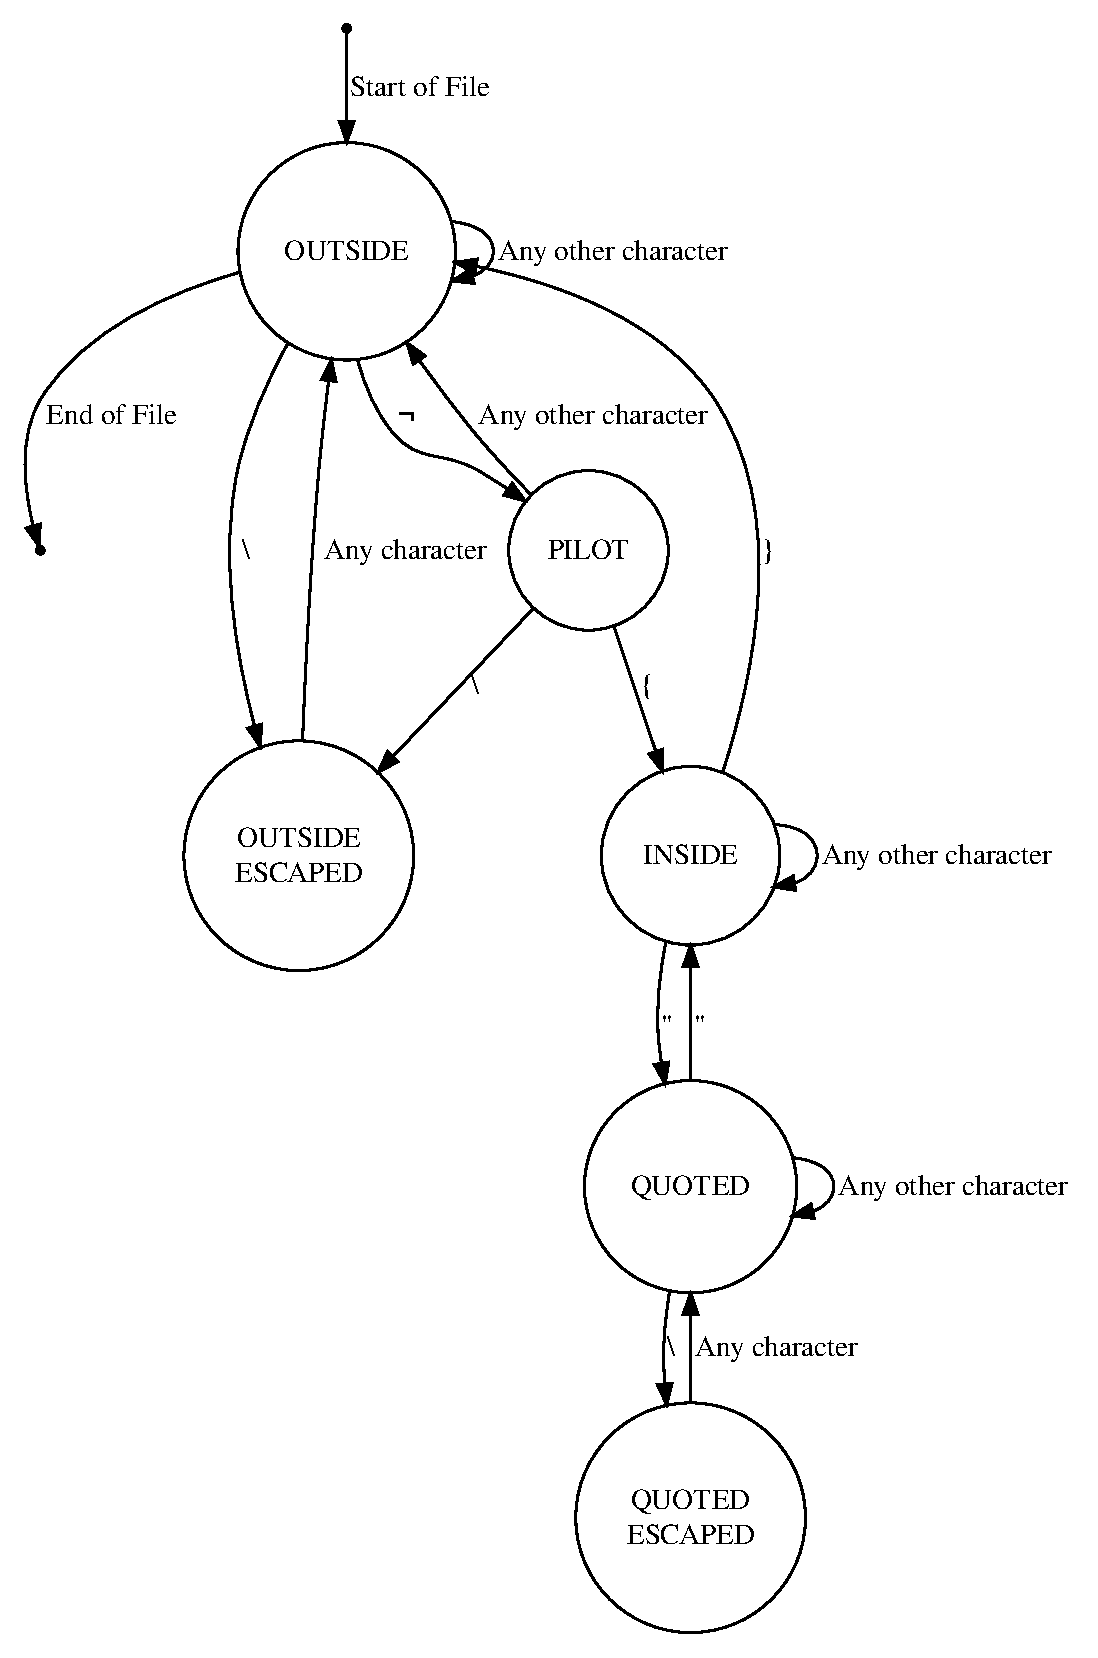
\includegraphics[width=130mm]{Figures/statemachine.eps}
\caption{\label{state machine}Placeholder state machine}
\end{figure}

\subsection*{Nodes and Node Types}
\label{gilt:parser:nodes}

Although an intermediate template document is on one level just a sequence of characters, this is not a very useful abstraction for understanding the intent of the template and converting it to another form. Instead, this parser examines the input document and converts it to a collection of `nodes'. Each node represents some part of the input document. The Nodes have been chosen, wherever possible, to align with the key concepts of template languages. Each node should contain enough information to enable it to be rendered into an equivalent concept in the target template language.

The nodes produced by the parser form a broad-based tree structure. The root of the tree is a sequence of nodes representing the `top level'. This level includes nodes such as text nodes representing boilerplate text and lookup nodes representing a value to be inserted in the output when a template is expanded. Some of these top-level nodes, however, may include other nodes within them. For example, a conditional node requires a discriminator value, which will usually be a lookup node. The action or actions associated with the conditional node might be other nodes such as a text node representing literal text, a block reference node with the name of a block to render, a template inclusion node, and so on.

Every node implements a single Java interface, shown below.

\begin{lstlisting}[backgroundcolor=\color{black!5},escapeinside={(*}{*)},tabsize=2,label={gilt:Node.java},caption={Parser Node interface},captionpos=b]
public interface Node {
	static final String VALUE = "value";

	String getType();
	Map<String,Node> getContent();

	default Node get(String key) { return getContent().get(key); }
	default Node getValue() { return get(VALUE); }
	default String getText() { return null; }
}
\end{lstlisting}

This allows each node to contain a collection of other named nodes, with one given priority as the `value' of this node to simplify code for the common case of boilerplate text and simple lookup or template inclusion nodes. Each node also has a `type' to enable the code in the template generator to decide what to do with the node and how to render it to the destination template language. The template generation code knows nothing about the individual classes which implement this interface, but deal exclusively in the Node interface and its methods.

The various node types produced by the parser have a lot in common. For ease of implementation, some of these similarities have been gathered into an abstract helper class \verb!AbstractNode!. All the implementing classes extend from this class in order to make use of its facilities. The \verb!AbstractNode! class provides an internal data structure to store the inner nodes as well as methods which the individual Node implementations can use to add inner nodes. In addition, the \verb!AbstractNode! class provides methods for diagnostic output which were used when testing the intermediate language parser.

The node types produced by this parser are as follows:

\paragraph{Text node}

A text node represents a block of plain text. This text may be boilerplate text, found between placeholders or at the start or end of the document, or it may be literal text found within the definition of a placeholder. In either case, the intention is the same. When generating a template in the target template language, a text template will be rendered as text. A text node has one internal value, the text itself.

\paragraph{Block Start Node}

A block start node represents the start of a named block. A block start node has one internal value, the name of the block. A block start node is always a top-level node

\paragraph{Block End Node}

A block end node represents the end of a named block. A block end node has one internal value, the name of the block. A block end node is always a top-level node.

\paragraph{Block Reference Node}

A block reference node represents the use of a named block. A block reference node has one internal value, the name of the block. Although a block reference node can be a top-level node, it is more usual to encounter it as the action associated with another node such as a conditional node or a loop node.

\paragraph{Lookup node}

A lookup node represents the fetching of a value from the template context. A lookup node has one mandatory internal value, the name of the value to look up. This node can also contain some optional internal values: a field to access, a method to invoke, and a collection of parameters for that method. In the initial implementation of the intermediate language parser, field and method access are exclusive, so a lookup node can contain a field name, a method name, or neither. Method parameters can only be present if a method name has been specified. The context value name, field name, and method name are all simple text values, but the collection of method parameters can include multiple parameters and those in turn can be literal values or other nodes. The collection of method parameters is represented as an array node (see below).

\paragraph{Template Inclusion Node}

A template inclusion node represents the inclusion of one template by another. The single internal value is a Node representing how to find the name of the template to include. In the initial version of the intermediate language and the parser this internal value can be either a literal text node or a lookup node. More complex configurations such as including a template whose name is given in a file are not supported.

\paragraph{Conditional Node}

A conditional node represents a decision within the template. A conditional node has one mandatory internal value, a node representing the discriminating value. Although the intermediate language allows this to be a literal, that would usually be a pointless exercise, as the result of the conditional expression would always be the same. For most uses this internal value will be a lookup node representing the context value on which to make the decision.

A conditional node can also have a combination of three optional values. If a value was specified using the \verb!is! keyword then that value will be stored as an internal value to be matched. If an action was specified using the \verb!then! keyword then that value will be stored as an action to be performed if the discriminating expression is `true'. If an action was specified using the \verb!else! keyword then that value will be stored as an action to be performed if the discriminating expression is `false'. The initial implementation of the parser does not prevent the declaration of a conditional placeholder with neither a \verb!then! nor an \verb!else! action. If neither are present, then the conditional node will perform no action and produce no output when the destination template is expanded. The nodes representing the actions will usually be block reference nodes, template inclusion nodes, or literal values.

\paragraph{Loop Node}

A loop node represents an iteration placeholder. A loop node has one mandatory internal value, a node representing the collection to be iterated through. While this could potentially be a literal, the initial intermediate language has no syntax to specify multi-value literals, so that is not likely to be a valid type to be iterated in the destination template language. In most cases the node representing the collection will be a lookup node which specifies how to retrieve the collection from the template context. The action to be performed for each element of the collection, specified using the \verb!do! keyword, is theoretically optional, although a loop with no action would generate no output when the destination template is expanded. The node representing this action will usually be a block reference node, a template inclusion node, or a literal value. Two extra internal values are also optional. If a symbol is specified using the \verb!with! keyword it will be stored for use when the destination template is generated. If an element separator is specified using the \verb!separator! it will be also be stored as an internal value. The separator value can be any of the action node types used for \verb!do!, above.

\paragraph{Method Call Node}

A method call node represents a method call placeholder. Although this type of node was supported in the initial intermediate language, and thus the initial parser and generator implementations, it was later subsumed into the lookup node, In the initial implementation it had two mandatory internal values, a lookup node representing the context value on which to invoke the method and a literal value containing the name of the method. As with the method call option of the lookup node, there was also the option to include a collection of parameters. If present, they were stored using an array node.

\paragraph{Array Node}

An array node is an internal node which cannot appear as a top-level node. An array node is created whenever another node needs to contain an unknown number of internal values. Specifically, in the initial implementation of the template language model it is used to contain the list of nodes representing method parameters in both lookup nodes and method call nodes.

\paragraph{Reference Node}

As discussed above, for the intermediate language to express the notion of a current loop element in a way which is independent of the destination template language, it requires a symbolic way to indicate when the current loop element is to be mentioned during template generation. This is the purpose of the reference node. A reference node is produced when a placeholder which starts with the \verb!reference! keyword is parsed. A reference node has one internal value containing the name of the symbol to be referenced. If no symbol name is specified in the reference placeholder, the default value of `this' is used.

\paragraph{}

\subsection*{Character Buffering}
\label{gilt:parser:buffering}

As discussed above, the aim of the intermediate language parser is to convert an incoming template into a sequence of nodes representing the parsed components of the template. Each node typically represents a block of characters from the input template. Each chunk of boilerplate text is represented as a single node, regardless of the length of the chunk. Likewise, each placeholder is represented as a single node with internal values indicating the type of placeholder and the combination of directives and values within it. In both these cases, the content of the node to be constructed is not known until the end is reached. The end of a chunk of boilerplate text is indicated either by the end of the input or by the start of a placeholder. The end of a placeholder is indicated by the terminating \verb!}! character.

The intermediate language parser includes a buffer to collect the text which will ultimately be converted to a node of one sort or another. From the start of a chunk of boilerplate text, or the start of a placeholder, incoming characters are accumulated into a buffer. At the end, the contents of the buffer are converted to a node. Accumulated boilerplate text is directly converted to a text node. Accumulated placeholder text is passed to a separate \verb!PlaceholderParser! object which processes the contents of the buffer according to the grammar of placeholder contents. When the node has been created, the buffer is cleared ready to begin collecting characters for the next node.

Adding text to the buffer normally happens on the `any other character' transitions when the state of the state machine (INSIDE or OUTSIDE) remains the same. Special characters such as placeholder delimiters are not usually added to the buffer, as they serve to indicate the start or end of a node. However, here are a few situations in which special characters are added to the buffer. Any `escaped' characters are added to the buffer, although the escape character (\verb!\!) is not. Quote characters (\verb!"!) in placeholders change the state for the purposes of parsing, but are added to the buffer along with the rest of the placeholder characters. The most complex case is if a `pilot' character (\verb!¬!) is encountered but it is not followed by the \verb!{! which would complete the start of a placeholder (or there is a \verb!{!, but it is escaped). In this case, both the pilot character and the current character need to be added to the buffer. This is the only case in which the parser needs to `undo' a decision while parsing.

\subsection*{Parsing of Placeholders}
\label{gilt:parser:placeholders}

Once the enclosing \verb!¬{! and \verb!}! have been stripped off, each placeholder consists of a sequence of characters which need to be parsed according to the placeholder grammar to determine which specific node or nodes to create. A formal specification for the placeholder grammar is given in \autoref{appendix:bnf initial}. Within a placeholder, unquoted whitespace characters are not significant and are removed as the placeholder contents are parsed. In the following discussion of the parsing process, such whitespace will be ignored. 

As mentioned above, the keywords in the intermediate language have been carefully chosen so that they all have distinct starting letters. The top-level `action' symbols which can start a placeholder, and the node classes which result are shown in the table below. A placeholder that starts with any character not in the table is invalid. A parse error will be produced and parsing will stop.

\begin{table}[ht!]
\fontsize{9}{11}\selectfont
  \begin{center}
    \begin{tabular}{rlll}
      \textbf{Character} & \textbf{Keyword} & \textbf{Description} & \textbf{Node class} \\
      \toprule
      \multicolumn{4}{c}{Top-Level Keywords} \\
      \textbf{i} & \verb!if! & conditional & \verb!IfNode! \\
      \textbf{f} & \verb!foreach! & loop & \verb!LoopNode! \\
      \textbf{s} & \verb!start! & block start & \verb!BlockStartNode! \\
      \textbf{e} & \verb!end! & block end & \verb!BlockEndNode! \\
      \textbf{b} & \verb!block! & block reference & \verb!BlockNode! \\
      \textbf{t} & \verb!template! & template inclusion & \verb!TemplateNode! \\
      \textbf{l} & \verb!lookup! & value lookup & \verb!LookupNode! \\
      \textbf{r} & \verb!reference! & symbol reference & \verb!ReferenceNode! \\
      \textbf{"} & & \emph{quoted literal} & \verb!TextNode! \\
      \hline
      \multicolumn{4}{c}{Context-Specific Keywords} \\
      \textbf{d} & \verb!do! & loop body & \emph{various} \\
      \textbf{e} & \verb!else! & action if false & \emph{various} \\
      \textbf{i} & \verb!is! & conditional match value & \verb!TextNode! \\
      \textbf{f} & \verb!field! & lookup field name & \verb!TextNode! \\
      \textbf{m} & \verb!method! & lookup method name & \verb!TextNode! \\
      \textbf{p} & \verb!parameter! & method parameter & \emph{various} \\
      \textbf{s} & \verb!separator! & loop separator & \emph{various} \\
      \textbf{t} & \verb!then! & action if true & \emph{various} \\
      \textbf{w} & \verb!with! & loop variable name & \verb!TextNode! \\
    \end{tabular}
  \end{center}
\caption{Keyword Initial Characters}
\label{gilt:table:initial characters}
\end{table}

The placeholder parser examines the initial character of the placeholder and calls an appropriate parse method for each placeholder type. This parse method is responsible for parsing the rest of the placeholder and returning a \verb!Node! object representing it. Each method (except for quoted literals which effectively have a single character keyword) begins with a call to a method \verb!expect! which is given the full text of the keyword, for example by calling \verb!expect("lookup")!. This method steps through the incoming character stream checking that the specified characters are present. If the keyword ends prematurely, or contains an unexpected character, then a parse error will be produced and parsing will stop. Once the initial keyword has been verified, the code for the parse method depends on the specific nature of that type of placeholder. The sequence of methods called to parse the remainder of the placeholder follow the grammar.

As a simple example, a block start placeholder is defined in the grammar specification as the keyword \verb!start! followed by a literal, so in the method for a block start, the keyword is verified, then the \verb!literal! method is called to parse a literal value. All the parse methods return a \verb!Node! object, including ones which cannot be used at the top-level of a placeholder, so in this case calling the \verb!literal! method results in a \verb!TextNode! object representing the literal text. As the literal value is the only extra node in this case, as soon as the \verb!TextNode! object is returned from the \verb!literal! method it is used as the value when constructing a new \verb!BlockStartNode! which is then returned from the parse method.

Block end and block reference placeholders also require a single literal value following the initial keyword, so the structure of their parse methods is similar to the block start method. Other parse methods are more complex, however, as they have options which need to be correctly recognised and processed. In such cases the process is similar to the process for the `action' symbol used at the top-level of a placeholder. The next character of the input stream is examined and checked against a list of valid options. If a valid initial character is encountered, then parsing is handed off to the appropriate parse method.

For example, the \verb!conditional! method is used to parse placeholders which start with \verb!if!. The placeholder grammar indicates that the next item must be a `value', so the \verb!value! method is called to return a \verb!Node! object representing that value. After the value, there are several optional items. The next item can be either \verb!is!, \verb!then!, \verb!else!, or nothing at all. A Node variable is prepared in advance for each option and set to \verb!null!, indicating that the particular option has not been provided. If the placeholder ends at this point, then the resulting \verb!IfNode! object will have no internal values for the value to match, the action on true, or the action on false. If the next character in the placeholder is one of \verb!i!, \verb!t!, or \verb!e!, then the process continues with an appropriate parse method, which follows the same pattern as all the parse methods. Call \verb!expect! to verify the full keyword, then combine the mandatory and optional following values into a \verb!Node! object which is then returned. Each returned value is placed into the variable prepared for that purpose. When the placeholder ends, the collected variables are combined into an \verb!IfNode! which is returned from the method.

The \verb!Node! objects resulting from top-level placeholders are then added to the sequence of nodes which represent the template as a whole, alongside any \verb!TextNode! objects resulting from boilerplate text. This sequence of nodes is what is passed to the template generator for rendering into a destination template.

The parsing approach described above correctly implements the placeholder grammar, but that does not mean that all possible combinations of nodes and sub-nodes are useful.  For example, as can be seen from the table of initial characters, a placeholder which starts with a double-quote character represents literal text and results in the creation of a \verb!TextNode! object. While this is legitimate according to the placeholder grammar, it is generally not very useful, as the resulting node is indistinguishable to the generator from a section of boilerplate equivalent to the quoted text. Likewise, an \verb!ifNode! with none of the optional values, although valid, represents a template action that examines a value but does nothing with it, so it will not result in any output when the generated destination template is expanded. Depending on the syntax and semantics of the different destination template languages, such pointless constructs may not even be able to generate valid templates.

\section*{The Template Generator}
\label{gilt:generator}

The job of the template generator is to take a template expressed in the intermediate language and convert it, where possible, to a similarly-functioning template in a destination template language. Conversion is not always possible, however. The intermediate language is designed to support a set of common template language features but these are not supported in all template languages.

There is only one intermediate language, so the template generator creates an instance of the intermediate language parser which it uses to parse a supplied intermediate template to produce a sequence of \verb!Node! objects representing the various chunks of boilerplate text and placeholders from the original template. To produce a destination template, the template generator passes the parsed sequence of Nodes to a template language driver which understands how to render each type of Node into the syntax and grammar of the destination template language.

\subsection*{Template Storage and the Tract class}
\label{gilt:tract}

Different template engines have different requirements for template storage. Some template engines expect a template to be provided as a text string in memory, some require that every template exists in a file, sometimes with a specific filename, location or file type. The Template generator cannot know about the vagaries of every possible template engine, so an abstraction is required to isolate the generation process from such details.

The template generator treats every template as an object which implements the \verb!Tract! interface. The Tract interface provides a small set of methods to access the content (in this case the text of the template) and a collection of name/value properties. In this use of the \verb!Tract! concept, the properties depend on the requirements of the specific template engine. Some template engines will not need properties in addition to the text of the template, while others may require details of, for example, how and where the template should be stored.

When Tract objects need to be retrieved from storage, there is another abstraction \verb!TractSource!. \verb!TractSource! is also an interface which provides a method to retrieve a \verb!Tract! by name, and also some general purpose methods to enquire about the \verb!TractSource! itself, such as whether it is empty or where it is located. By default, a \verb!TractSource! is read-only, but a further interface \verb!WritableTractSource! extends this to support placing a \verb!Tract! into the store as well as removing a stored \verb!Tract! or clearing the store.

\verb!TractSource! (and \verb!WritableTractSource!) implementations can be created to represent the details of how and where templates are stored. The template generator can use the \verb!TractSource! methods on a provided store object with no knowledge of the underlying implementation.

\subsection*{Drivers and Dynamic Loading}
\label{gilt:plugins}

Using the same justification as the design of the dynamic loading mechanism for template engine drivers during template engine comparison (as described in \autoref{comp:plugins:dynamic}), each template language driver is implemented as a separate `plugin'. When generating templates for a particular template language, the plugin is specified as a command-line parameter which adds the plugin classes to the Java classpath of the running generator.

The template generator refers to a class named \verb!plugin.DriverFactory! which serves the same purpose as the class \verb!plugin.EngineFactory! described in \autoref{comp:plugins:dynamic}. All implementations of \verb!plugin.DriverFactory! implement a Java interface which specifies the methods it must implement. In a similar pattern to \verb!plugin.EngineFactory!, the interface implemented by template language drivers contains just two methods, as shown below.

\begin{lstlisting}[backgroundcolor=\color{black!5},escapeinside={(*}{*)},tabsize=2,label={gilt:DriverFactory.java},caption={Parser DriverFactory interface},captionpos=b]
package shared;
import java.io.IOException;
import com.efsol.templates.TemplateDriver;

public interface DriverFactory {
	TemplateDriver create() throws IOException;
	String getName();
}
\end{lstlisting}

As an example, the code for this class in the \emph{Trimou} plugin is shown below.

\begin{lstlisting}[backgroundcolor=\color{black!5},escapeinside={(*}{*)},tabsize=2,label={gilt:trimou:DriverFactory.java},caption={Trimou DriverFactory interface},captionpos=b]
package plugin;
import java.io.IOException;
import com.efsol.templates.TemplateDriver;

public class DriverFactory implements shared.DriverFactory {
    @Override
    public TemplateDriver create() throws IOException {
        return new TrimouTemplateDriver();
    }

    @Override
    public String getName() {
        return "trimou";
    }
}
\end{lstlisting}

\section*{Potential Improvements to the Intermediate Language}
\label{gilt:language plus}

\paragraph{Redefinable Delimiters}
The choice of characters to delimit the start and end of placeholders was largely arbitrary, based on locating a character sequence not significant in the available template languages and not common in content for common document types. This choice raises some issues, however. One problem is that the initial `pilot' character \verb!¬! is not available on all keyboards. Although more common, the \verb!{! and \verb!}! can also be difficult to enter on a range of keyboard layouts \citep{Erz2023a}. It is usually possible to enter these characters if needed, but the methods can be clumsy, such as entering a multi-digit character code, or copying the character from elsewhere and pasting it into the text. This can make working with intermediate templates far from the intended comfortable experience. Another problem is that if a desired target document type \emph{does} use these characters, then frequent escaping will be required, with any failure to escape these characters leading to errors and invalid templates.

Without knowing every possible future keyboard layout or document type it is impossible to determine a `perfect' set of delimiter characters. To address these issues would require some way to redefine the characters to be used to delimit placeholders, allowing characters to be chosen which are both easy to type and minimise conflicts with document content. There are several ways to achieve this including: requiring users to change and re-compile the parser code itself; command-line parameters, configuration files, or other run-time parser settings; and configuration overrides associated with either individual templates or all templates retrieved from a particular template source location.

Global settings such as code-editing or configuration files persist between template generation runs and tend to have a relatively long life, so these approaches might be suitable for configurations related to hardware such as keyboard layouts. Such long-term settings would be less suitable for adapting to specific document formats, however. These might be better served by configuration overrides associated with individual or groups of templates.

Improving the intermediate template parser to support redefinable delimiter characters would require code changes to remove the dependency on literal delimiter characters in the code and to accept redefinitions from a range of sources. The initial implementation of the template parser and generator does not have any external configurations, so any external redefinition of these characters would require extra code to support that. One of the aims of the development was to create a system which is portable for many uses and situations, so relying on configuration mechanisms specific to particular operating systems or file structures would not be appropriate. An initial solution for persistent configurations which adapt the system to the local environment is to use command-line parameters. These are supported, in one form or another, by all common systems and can be made more-or-less persistent by including them in whatever script, shortcut, or desktop icon is used to launch the template generator.

The possibilities for setting overrides which apply just to one template or to a specific group of templates are just as varied. The same command-line options as for local environment settings can also be used for this task, but that is likely to lead to a proliferation of scripts and launchers and the concomitant increase in the risk of mistakes. Anther option includes some form of configuration file placed in the same location as some of the intermediate templates or with the same name as some of the intermediate templates. The system would then be able to look in this configuration file before attempting to process an intermediate template. While this system is plausible, it ties the configurations not just to the intermediate template contents, but to its name or location. If either of these are changed, then any associated configuration files would need to be changed to keep them in step. This approach also potentially slows down template processing, as the system would need to check for the existence of any associated configuration overrides before parsing, even if no such configuration overrides exist for that particular template. Similar problems would be faced by solutions involving a single centralised configuration explaining which configurations to use under which circumstances. To avoid such accidental coupling, it seems logical to place any configuration overrides which affect the processing of a template inside the template itself. With this approach, templates can be moved or renamed with no impact.

The challenge with including configurations within a file is to reliably distinguish them from the rest of the file's contents. For any configurations which do not affect the characters used as delimiters, this would be a relatively simple operation. Just introduce a new type of placeholder directive which allows the definition of a configuration, then include such directives before any other placeholders or directives which make use of the new configuration. This approach is arguably possible even for configurations which change the delimiter characters, but this would result in a template file containing both old and new delimiters and impose constraints on the order of the parsing process.

An alternative is to use a completely different syntax to indicate configuration settings. There is precedent for including such `header' text in a wide range of files, from the collection of name-value pairs found at the start of HTTP messages and emails, to delimited blocks of JSON or YAML data. The challenge is to unambiguously indicate the presence in such a header without assuming anything about the potential content of the file. HTTP and email documents do this by asserting that there will always be such a header, even if it is empty. The working assumption for this intermediate language is that such per-file overrides will be relatively rare, used only in the cases where the neither the default configurations nor any local command-line overrides are suitable for a particular file's contents. The overhead of always requiring a header seems too much for such rare cases, so a delimited approach seems more appropriate.

Typical JSON and YAML headers use repeated multi-character delimiters such as \verb!---! on a line of their own at the start and end of the header block, and also require the header block to be the very first content in the file. This enables a parser to quickly determine the presence or absence of the header block by analysing the first few characters in the file. There is, of course, always the risk that legitimate file contents might also start with this character sequence, but experience has shown that this is extremely rare. Even for cases of such a clash, the header block is only parsed once so placing an header block, which can be empty, at the start of a template would then allow the header prefix to be used within the template. An alternative approach would be to use the command-line configuration discussed above to define an alternative starting and ending sequence for such a configuration header.

This situation does not need many configuration options, so the structural overhead of JSON or YAML parsing seems unnecessary. A simpler name/value list, similar to HTTP and email headers would appear to be sufficient. An example intermediate template with a header block overriding the intermediate language delimiters might therefore look like:

\begin{lstlisting}[backgroundcolor=\color{black!5},escapeinside={(*}{*)},label={gilt:delimiter override},caption={Potential delimiter override syntax},captionpos=b]
---
delimiter start: %<
delimiter end: >
---
%<foreach lookup "prices" do template "price" separator ",">
\end{lstlisting}

Note that while the choice of starting delimiter can be anything which does not conflict with the boilerplate content, the choice of ending delimiter is limited to a single character which cannot appear unquoted within a placeholder or other directive.

\paragraph{Nested Blocks and Name Repetition}

In the intermediate language, named blocks are used to indicate sections of boilerplate and intermediate template markup which are used with control structures such as conditional and iteration directives. The design of the initial language allows these blocks to be nested with other named blocks, and in order to correctly detect and report on incorrect nesting or blocks without an end directive, both the start and end directive for each block must contain the same name. This approach is also used in HTML and XML markup \citep{Bray2008}. However, this requirement for the repetition of the name potentially increases the fragility of the language. Some other forms of markup chose only to indicate the name or type of a block at the start, and use a generic end for all blocks.

Although repeating the block name at the end has a range of benefits, such as making it slightly easier to find the other end of a block, or to remind a reader when a block is too long to take in all at once, the primary benefit of the repeated names is for error detection and reporting in the case of malformed nested blocks. While nested blocks can make more sense to some readers, as they can more closely mirror the expected structure of the generated template in some template languages, they are not strictly necessary for the template generation process to work correctly. All named blocks exist in the same namespace and will be located and used wherever they are positioned in a template.

If nesting of templates were to be prohibited, then the repetition of the name would no longer be so useful for error detection and reporting, and a more generic \verb!end! directive could be used.

\paragraph{Null Values and The Potentially Redundant Call Directive}

In the initial design for the intermediate language, code execution through method calls was envisaged as a separate concept to looking up a value from the supplied template context. Method calls have their own directive \verb!call!, distinct from the \verb!lookup! or \verb!template! directives allowed in value placeholders. Following use of the intermediate language, however, it became apparent that method calls were usually used as just a special case of value placeholder, especially when value placeholder processing was enhanced to allow field, method, and JavaBean access from context values.

If the intermediate language were being designed purely as a template language in its own right, this would not be an issue, the syntax for specifying method calls could be merged with that for value placeholders with no major impact. The main purpose of the intermediate language, however, is as a representation which can be automatically transformed into other template languages. Some of those other template languages do separate the two concepts. In the \emph{JSP} template language, for example, these two concepts even have different delimiters to distinguish them within templates \citep{Oracle2000}. The distinction exists because some methods are declared as not returning a value, so there will be nothing to put into the output document as a result of the method execution. Some template engines can cope with a placeholder which does not provide a value, treat it as if the placeholder had provided an empty string, and so render nothing into the output document. Other template engines will either fail to process the template, or insert some error message or other unwanted text into the output document. Such template engines, if they support method calls at all, usually require a separate syntax to indicate that the method is not expected to return a value and therefore does not provide any text to include in the output document.

At the time at which the intermediate template is processed to generate the `real' templates, nothing is known about run-time details such as whether a method call will return a value, or whether a context value or field will be null. Arguably the intermediate language should provide a way for template authors, who may know more about what is supposed to happen when the target template is expanded, to indicate in the intermediate language markup whether a method call is expected to return a value, so that the generation process can select appropriate syntax when generating a template. In the initial design for the intermediate language, the separate `call' directive provides a way to indicate this, but the behaviour is implicit rather than explicit and may not be obvious to a template author who is not familiar with how the generation process works.

A better solution to this issue would be to merge the value placeholder and method call syntax, but allow optional explicit markup on any placeholder to indicate that it is not expected to provide a value for the output. A potential syntax for this might look like:

\begin{lstlisting}[backgroundcolor=\color{black!5},escapeinside={(*}{*)},label={gilt:lookup method call},caption={Potential merged lookup method call syntax},captionpos=b]
(*¬*){lookup "product" method "price" parameter "GBP" void}
\end{lstlisting}

where the keyword \verb!void! indicates that either the method returns no value, or that the value should be discarded and not added to the output document.

\paragraph{Explicit Types for Context Values and Method Parameters}

Most template languages, and the template engines which implement them, are `weakly typed' - they have only a loose notion of data types. In such languages, a data item is required to have a value which can be represented as text, but the actual type of the value is largely unimportant. This becomes a little more complex when the template language supports features such as field access, list element iteration, or method calls. These actions require an object of a type which supports such operations, but this is usually only checked when the action is executed during template expansion. An attempt to, for example, access a named field of an object which does not have a publicly available field of that name will result in some form of error or warning when the template is expanded. This may, in turn result in no value appearing for that value, an error message of some sort appearing in the output document, or the template failing to expand at all. Although they are less common, with only one example in the cohort of template engines under consideration for this research, some template languages are `strongly typed' \citep{Fokkinga1981} \citep{Madsen1990}. This kind of template language requires that all context variables and other data values have an explicit associated type. Any attempt to use a value with an incorrect type can then be caught at the start of template expansion.

The initial version of the intermediate language does not support typed values, nor any way to refer to non-core classes, so for strongly-typed template languages it is assumed that all values are of type String. This obviously works only if the values are actually of type String, and will generate an incorrect output template whenever different types are required. To address this issue, and enable the template generator to produce correct templates for strongly-typed template languages the intermediate language would need enhancement to allow specification of value types. These type specifications would not be required or used when generating templates for weakly typed template languages. For practicality, it would seem reasonable to make such annotations optional, only required when the value datatype is other than String. Potential syntax for this might look like:

\begin{lstlisting}[backgroundcolor=\color{black!5},escapeinside={(*}{*)},label={gilt:variable types},caption={Potential value type syntax},captionpos=b]
(*¬*){lookup "stocklevel" type "java.lang.Integer"}
\end{lstlisting}

This indicates that the context value stored with the name `stocklevel' is of type `java.lang.Integer'. All types starting with `java.lang.' (indicating that they are part of the `java.lang' package) are built-in types in Java and do not need an `import' directive. Where no package is specified, it is assumed to be `java.lang', so this type could also have been written as `Integer'.

A similar approach would also be suitable for method calls, as shown below.

\begin{lstlisting}[backgroundcolor=\color{black!5},escapeinside={(*}{*)},label={gilt:parameter types},caption={Potential type syntax for method calls},captionpos=b]
(*¬*){lookup "product" type "com.shirtshop.Sku" method "price" parameter "GBP"}
\end{lstlisting}

In this case the context value stored with the name `product' is defined to be of type \verb!com.shirtshop.Sku!. As the type name does not start with \verb!java.lang!, it indicates an external class which would need an \verb!import! declaration in a strongly-typed template language such as \emph{JTE}. The template engine which processes such a template would then be able to determine whether the `product' object exposes a method named `price' prior to attempting to call the method.

\paragraph{Constants and Variables}

In a general-purpose programming language it is very common to give names to intermediate values. This both assists with the readability of the code and enables these values to be re-used without the need for recalculation. Template languages often borrow features from general-purpose programming languages so it should come as no surprise that some template languages also have this feature. Most general-purpose programming languages make the distinction between a `constant', whose value is defined to remain the same for the whole execution of a program, and a `variable' which may be later redefined to a different value. These concepts are not universally applied, however. Some programming languages, such as \emph{Haskell}, treat all values as immutable and so do not really have the concept of variables \citep{Marlow2010}, while others, such as \emph{Lisp} treat everything as changeable, even the program code.

A template language is not the same as a general-purpose programming language, however, as it lacks the concept of sequential execution which characterises most general-purpose programming languages. Conceptually a template is all evaluated at once. This makes the key characteristic of variables - that they may change over time - a difficult concept to determine. Template engines address this in a variety of ways. Some, typically the ones which compile a template into a program, method, or subroutine in a general-purpose programming language as a first step in expanding it, embody the assumption that a template is evaluated top-to-bottom. In such a model, variables make sense and the same variable name can be redefined to take different values as the template is processed. Others, typically ones in which a template is parsed into a tree or other internal representation as a first step in expanding it, may evaluate placeholders and other template expressions in an arbitrary order. In such a model, variable life-cycles do not make sense, so where such template languages support named intermediate values they are usually immutable and more like constants than variables, even if the syntax implies variability.

It would be possible for the intermediate language to support named intermediate values to be rendered as variables in the target template language, but the semantics of the template variables would depend entirely on the template engine which eventually evaluates the generated template. It would also be possible for the intermediate language to support constants or variables which are not passed through to be rendered as variables in the target template language but instead used by the intermediate language itself during the generation of templates. The main advantage of this would be similar to the approach of naming blocks within the template - to increase readability and to enable re-use of common template expressions without the need to redefine them multiple times. In this sense such a definition would be more akin to a `macro' than a more traditional constant or variable.

An potential syntax for named values might look like:

\begin{lstlisting}[backgroundcolor=\color{black!5},escapeinside={(*}{*)},label={gilt:variables},caption={Potential variable definition syntax},captionpos=b]
(*¬*){define "cost" as lookup "product" method "price" parameter "GBP"}
\end{lstlisting}

In this case a value named `cost' is defined as the result of calling the method `price' with a single String parameter `GBP' on the context object with the name `product'. The defined value can then be referenced in a regular \verb!lookup! directive, as if it is stored in the template context. When generating a template in a language which supports such named values, this can be rendered using the appropriate syntax. When generating a template in a language which does not support named values, the template generator will fall back to rendering the complete value expression wherever it is used, in the style of a macro.

\paragraph{Non-literal Parameters to Methods}

The initial implementation of the intermediate language has inconsistent support for indirect values. For example, it supports the use of a context value as the name for a template to be included. However, initial support for method calls was based on calling \emph{JavaBeans} or other methods without parameters. Method parameters were added later in development and are always assumed to be literal values. While literal parameters may make sense for some specific cases, in the general case it is likely that some methods will need parameters which are different for different uses of the template and should therefore be stored in, and retrieved from, the template context. A more consistent approach to method parameters would allow for context values as parameters and possibly even indirect context values such as using the context value as the name of another context value. A potential syntax for such parameters might look like:

\begin{lstlisting}[backgroundcolor=\color{black!5},escapeinside={(*}{*)},label={gilt:lookup params},caption={Potential non-literal parameter syntax},captionpos=b]
(*¬*){lookup "product" type "com.shirtshop.Sku" method "price" parameter lookup "currency"}
\end{lstlisting}

This approach is not without its own issues, however. If the syntax were to be fully extended to also support method calls as a way to provide method parameters, there is the potential for confusion as to which method `owns' each parameter. In most general-purpose programming languages, this is addressed by the use of parentheses or other delimiters to group the parameters for a particular method call. So far, the design of the intermediate language has been suitable for deterministic parsing without the need for such delimiters, and adding them could add unwanted complexity to the parser and thus the template generation process. A similar problem could also occur with field access specifiers.

Support in destination template languages for any kind of method calls is not universal (see \autoref{fs:table:features}), and support for complex features, such as the use of the results of method calls as method parameters, is rarer still. If the intermediate language were to forbid method calls and field access in method parameters for the sake of faster and more deterministic parsing it is not clear how much this might impact real usage. If the intermediate language were to support context values as parameters, then in many cases the result of the subsidiary method call could be pre-calculated and placed into the template context or set as a template `variable' as described above.

\paragraph{Direct Access to Collection Elements}

As well as simple values, field access, and method calls, some template languages, such as \emph{Velocity}, support additional options on lookup placeholders. One such additional option is the ability to access indexed elements from arrays and other ordered collections. The \emph{Velocity} template fragment shown below represents accessing the first element from an ordered collection or array stored in the template context with the name `releases'.

\begin{lstlisting}[backgroundcolor=\color{black!5},escapeinside={(*}{*)},label={gilt:arrays},caption={Potential collection element syntax},captionpos=b]
$releases[0]
\end{lstlisting}

Internally within the \emph{Velocity} template engine this is translated to an appropriate way to access the element from the value. If the value is an array, then the Java array element syntax is used. If the value implements the \verb!java.util.List! interface, then a \verb!get()! method is called on the object passing in an integer to indicate the position in the list. This same syntax is also used for accessing values from an associative array. If the value implements the \verb!java.util.Map! interface, a similar \verb!get()! method is used to retrieve the value associated with a specified key.

The initial implementation of the intermediate language does not support this feature. Although the associative array aspect of this functionality can be emulated using the lookup method call syntax, all keys must be text strings, as there is no way to specify a literal integer value. As with so many features found in specific template languages, it is not clear how often this feature is used in live templates, or whether there is any way to effectively emulate it in template languages which do not support this feature.

\paragraph{Abbreviated Keywords}

During development of the intermediate template language parser there was a discussion about whether to also allow abbreviated or misspelled as well as full keywords. They all have unique initial letters so there would be no ambiguity. This was a technique used in many early implementations of the BASIC programming language \citep{Kurtz1978}, and using just the initial letter of each keyword could considerably reduce the amount of typing for template authors and the size of the intermediate templates. It would not, of course, have any effect on the size of the generated templates. The disadvantages of such an approach would be the potential loss of readability of templates expressed in this language and the need for whitespace or other delimiters to indicate the end of a keyword. This feature is still under consideration, and the initial implementation of the template generator requires full keywords.

\section*{Template Language Drivers}
\label{gilt:drivers}

The aim of the design of the intermediate language is that, after parsing the intermediate template, the resulting data structure contains all the information required to generate an equivalent template in each of the supported template languages. Subject, of course, to the capabilities of the individual template languages. In order to generate the destination templates, however, a mapping is required between the collection of symbolic language nodes held in the data structure, and the textual expression in a particular target template language. For this research, this mapping has been defined in the form of a range of software \emph{drivers}, written in Java. A separate driver has been created for each of the template engines in the cohort. All the template language drivers implement the same Java interface definition, which provides methods to render specific node types from the symbolic model.

\subsection*{Driver Interface and Shared Code}

In conjunction with the initial intermediate language and its parser, a Java interface was defined to provide a set of methods which all template language drivers must implement. The code for the interface is given below.

\begin{lstlisting}[backgroundcolor=\color{black!5},escapeinside={(*}{*)},tabsize=2,label={gilt:interface},caption={TemplateDriver interface},captionpos=b]
public interface TemplateDriver {
	void init(Map<String, Node[]> blocks, WritableTractSource templates);
	String renderNodeArray(Node[] nodes) throws IOException;

	void renderIncludeNode(String templateName) throws IOException;
	void renderBlockReferenceNode(String blockName) throws IOException;
	void renderIfNode(Node key, Node match, Node iftrue, Node iffalse) throws IOException;
	void renderLoopNode(Node target, Node with, Node body, Node sep) throws IOException;
	void renderTextNode(String text) throws IOException;
	void renderLookupNode(Node target, Node field, Node method, Node parameters) throws IOException;
	void renderMethodCallNode(Node target, Node method, Node[] parameters) throws IOException;
	void renderReferenceNode(Node symbol) throws IOException;

	String quote(String text);
}
\end{lstlisting}

In this interface there are three groups of methods. 

The first group consists of methods relating to the whole template generation process.

The \verb!init! method begins the generation process for a new output template. The parameters are a Map of nodes representing the named blocks from the intermediate template and a `place' where templates are stored. The `place' is a virtual location which provides a basic set of operations and can be implemented in different ways, such as a file store, an in-memory store, or even a remote store in a database or server if required.

The first parameter to this method is used during template generation whenever a control structure in the intermediate template refers to a named block. The contents of the block can be fetched from the supplied Map by name as an array of parse nodes and rendered in whatever manner and to whatever location the particular template language driver requires. The second parameter will be used for two situations. The first is if a `template' directive is encountered but the destination language does not support template inclusion. In this case, the template generator will need to render the contents of the included template directly into the output template. The second situation in which the template location will be needed is if the destination template language requires the generation of multiple template files rather than including the block contents in-line in the main template. This location is where generated sub-templates will be placed.

The \verb!renderNodeArray! method is used when rendering either a whole template or a sub-template such as a named block. This method is the main entry point into the driver from the template generator code. This is a separate method from the rest of the `render' methods as, depending on the destination template language and whether it is a `top level' template, the result may be included in the generated template, or it may be stored to the template `place' for direct use or for later inclusion when another template is expanded. The \verb!renderNodeArray! method returns the result as a text string which can then be stored or included as required.

The second group of methods are the core methods of the template language driver for each different template language. Each of these methods handles one of the types of nodes produced during parsing and allows the driver to render that type of node in an appropriate manner for that template language. The method names largely follow the node names and the syntax of the intermediate template language.

The \verb!renderIncludeNode! method allows the template language driver to adapt to the destination syntax for template inclusion and is triggered by the presence of a parse node resulting from a \verb!template! directive.

The \verb!renderBlockReferenceNode! method allows the template language driver to adapt to the destination syntax for sub-templates and is triggered by the presence of a parse node resulting from a \verb!block! directive.

The \verb!renderIfNode! method allows the template language driver to adapt to the destination syntax for conditional control structures and is triggered by the presence of a parse node resulting from an \verb!if! directive.

The \verb!renderLoopNode! method allows the template language driver to adapt to the destination syntax for loop control structures and is triggered by the presence of a parse node resulting from a \verb!loop! directive.

The \verb!renderTextNode! method is triggered by the presence of a parse node resulting from boilerplate text. Note that the parsing process also produces text nodes for literal text within a placeholder but these are handled within the render method for the appropriate placeholder directive.

The \verb!renderLookupNode! method allows the template language driver to adapt to the destination syntax for context value access and is triggered by the presence of a parse node resulting from a \verb!lookup! directive.

The final group of methods enable drivers to adapt to different situations during the processing of nodes.

The \verb!quote! method allows the template language driver to generate quoted and/or escaped text according to the rules for the destination template language.

\subsection*{Commonalities Between Template Languages}

While it would be possible to create a template language driver completely from scratch, based solely on the \verb!TemplateDriver! interface, the resulting code would likely have a lot of similarities to other drivers. This is for three main reasons. The first reason is that there is always a certain amount of general processing which will be needed in all implementations. For example, the code to step through the nodes in an array during processing of the \verb!renderNodeArray! method is very likely to be the same for most, if not all, template language driver implementations. The second reason is that, even in areas where template languages differ, they are not entirely distinct from each other. Some template languages will have similar syntax to others for some operations, or the structure of their syntax will be similar enough that portions of the code to generate the resulting template will be the same. For example in this cohort of template engines, \emph{Handlebars}, \emph{Hapax}, \emph{Jangod}, \emph{Mustachej}, \emph{Pebble}, and \emph{Trimou} all use the same basic syntax for context value placeholders. In this case, the code for value placeholders in all these different driver implementations will probably be functionally identical. A third reason for similarity of code is that the intermediate language is capable of expressing some relatively complex template directives and expressions which only a few template languages support. In these situations, the code for most of the template drivers will consist of an error message indicating that the destination template language cannot support the required construct. If most template languages do not support a particular combination of features, then they could all make use of the same default implementation which produces such an error message.

In cases where there is some similarity between template languages, it can make sense to share code. In the initial implementation of the template generator, all the template language drivers share a base implementation of the \verb!TemplateDriver! interface named \verb!CommonTemplateDriver!. This class defines a default implementation for all of the `render' methods as well as a selection of helper methods to perform operations common to several template language driver implementations.

One of the key methods provided by this class is \verb!renderNode! which examines a supplied node and calls whichever of the other `render' methods is appropriate. This method understands the structure of each of the node types and is able to recognise each node by its `type' field and extract their options and parameters and construct a correct call to one of the specific method to render the node. This method will issue a template generation error if an unknown node type is encountered, but this should never happen unless the parser code is altered without corresponding changes to \verb!CommonTemplateDriver!. In addition to this basic functionality, the \verb!renderNode! method, along with most methods in the \verb!CommonTemplateDriver! class, provides switchable diagnostics to assist a driver author in verifying and debugging driver behaviour.

Some method implementations will be similar for almost all template language drivers. An example of this is the \verb!renderTextNode! method. All the template languages in this cohort render boilerplate text as-is, so the default implementation is very simple - it just adds the supplied text to the output template. There is a slight complication with this method, though. the specification of the initial intermediate language allows any characters which do not introduce an intermediate language placeholder in the boilerplate text. There is a chance, therefore, that boilerplate text may conflict with the placeholder syntax of the destination template language. In such cases, individual drivers can override this method to apply language-specific escaping rules to the supplied text before passing it on to the default method for rendering.

In addition to these key rendering methods, the \verb!CommonTemplateDriver! class also provides a range of overridable methods for common functions such as quoting or escaping text, or appending characters to the generated text in a variety of situations. For example, some template languages require the names of context values included templates to be quoted while others do not. Likewise, some template languages support literal text in place of context values, but these need to be quoted, and perhaps in a different way to template or context value names. The parsed node list resulting from parsing an intermediate template in the intermediate language contains a range of types of nodes including the various kinds of template directives and boilerplate text found outside placeholders. The code to determine when and how to quote or escape the textual values of these nodes could end up repeated in many drivers, so helper methods are provided which deal with common cases. The aim is to provide enough support that drivers only need to include code which is specific to that particular template language.

In the initial implementation of the template generator there is still work to be done in minimising the code requirements for each driver. There are areas where functionally identical code is included in all template drivers. For example, consider the implementation of the \verb!renderBlockReferenceNode! method from the \emph{Velocity} driver shown in \autoref{renderBlockReferenceNode}. This implementation contains no code specific to the \emph{Velocity} template language, and similar implementations are found in the drivers for other template languages. This code should therefore be moved to somewhere accessible to all drivers. Examining the template languages in the cohort under consideration, it appears that most use some form of in-line representation for code blocks, so this implementation is also a candidate for a default method implementation. This would allow most drivers to just use the default, and only drivers for template languages (such as \emph{Stringtree} and \emph{Solomon}) which use a different approach will need to implement this method.

\begin{lstlisting}[backgroundcolor=\color{black!5},escapeinside={(*}{*)},tabsize=2,label={renderBlockReferenceNode},caption={\emph{Velocity} implementation of `renderBlockReferenceNode'},captionpos=b]
@Override
public void renderBlockReferenceNode(String blockName) throws IOException {
    Node[] block = blocks.get(blockName);
    if (null == block) {
        throw new TemplateCompileError("attempt to reference unknown block '" + blockName + "'");
    }
    renderNodeArray(block);
}
\end{lstlisting}

\section*{Testing Template Generation}

All software needs to be tested in order to both prove correct operation and to discover any issues which need to be addressed or could be improved. This template generation software consists of three key components: the parser for the intermediate language; the template generator, and the individual drivers for the different template languages. Each of these components were tested separately. This required the construction of some extra software. To prevent unnoticed regressions, tests for these components were automated through writing code in Java using the JUnit \footnote{https://junit.org/junit5/} test libraries. Additional software was also written to provide `test stubs' for any parts of the system which were not being tested at that time. One of these `test stubs' was a `fake' template driver which could be used by the template generation process during testing. This template driver generated its own output designed for easy recognition and checking rather than attempting to match any real template language. The use of a test stub for this purpose rather than a real driver meant that any later changes to real drivers would not cause other tests to fail.

\subsection*{Testing the Intermediate Language Parser}

The parser for the intermediate language is a relatively complex piece of software which needed to evolve with the design of the intermediate language itself. Tests for the parser form three rough groups: syntax tests, placeholder tests, and grammar tests. Syntax tests include testing for correct recognition of empty files, boilerplate text without placeholders, and placeholders without boilerplate text. This group of tests also includes testing for correct error output in the case of incorrect intermediate language syntax such as incomplete placeholders or quoted text.

Placeholder tests for the intermediate language parser were more numerous, as there were more combinations and possibilities to be considered, even though they only concentrated on the parsing of the contents of a single placeholder. All the placeholder tests were constructed in a similar style. An object of the class \verb!PlaceholderParser! was created and provided with a text string containing the textual contents of a placeholder to be parsed, then the \verb!parse! method of the object was called to return a parsed \verb!Node! object. If no errors or exceptions were produced, the contents of the Node were then examined to check that the placeholder had been correctly parsed. Each type of placeholder had a set of tests covering valid and invalid content. Tests for valid content included checking the presence and absence of optional directives and values as well as checking with different types of values such as `lookup' values and quoted literal values.

Grammar tests include tests for the correct arrangement of placeholders and boilerplate text, for example, checking that each block start has a matching end. These were mostly tested as part of the template generation process, using the fake template driver and checking both that no errors were produced and that the correct output template was produced.

\subsection*{Testing the Template Generation Process}

The tests for the template generation process built on the intermediate language parser tests. Having determined that the parsing process was generating the correct nodes from both boilerplate text and placeholders, the next step was to ensure that the sequence of nodes representing the parsed template was being analysed correctly and passed to the appropriate driver methods for rendering. All the template generation tests were constructed in the same style, and a helper method was created to contain common code to minimise the size of each test. Before running any of the tests a template driver factory object for the fake template driver was created. At the start of each test a memory-based template storage `place' was created and a template driver was created using the template driver factory which was already available. When the driver had been created, a \verb!TemplateCompiler! object was created and its \verb!compile! method called, passing in the details of the template storage and the text containing a complete template to be processed. To complete the test, the generated template or templates were then retrieved from the template storage and compared with the expected result.

\subsection*{Testing Real Template Drivers}

Having determined that the parsing and template generation process was functioning correctly, the next step was to write and test the drivers for the rest of the template languages. This testing took place in several phases. The first phase was to code the driver and ensure that there were no compilation errors or run time problems when it was called by the template generator. The next phase was to perform a basic test using a standard, if relatively simple, input intermediate template which includes a range of text and placeholder types. Each driver test began by creating and initialising the template generation system, the driver, a template context, and the template engine being tested. With everything set up, the basic intermediate template was passed to the template generator to produce a destination template which was then expanded to produce a final document. This document was then checked to ensure that the resulting document contents were correct.

Beyond that, testing of each template driver needed to be specific to the template language being generated. Not only did the form and content of the generated template vary between template drivers, but each template language supported a different subset of the possible features available in the intermediate language. For these advanced features, the test suite for each driver contained a different set of tests, ensuring both that supported language features were correctly processed and that unsupported features produced a reasonable error message.

\section*{Discussion and Conclusions}

This research explored the possibility of creating an intermediate language to represent common template features in a way which could be used to generate templates for a range of template engines. On the whole, this exercise was a success, with the GILT language capable of expressing all the required features, and the tooling capable of generating equivalent templates for all the supported template engines, subject to their capabilities.

The initial version of the intermediate language still had some problems, though, including an arguably poor choice of delimiter syntax, a simplistic notion of value types, and potentially ambiguous interpretation of complex scenarios involving method parameters. Improvements to address these and other issues will be considered for a future version of the language and tooling.

The language and tooling were, however, able to be used for the performance and energy comparisons of more complex template scenarios as discussed in \autoref{chapter:comp energy}.



\end{appendices}

%\listchanges
\renewcommand\chaptername{Submission Notes} % for fancy headings, please do not change 
\chapter*{List of Corrections}

\newcommand{\p}[1]{\pageref{#1}}

\begin{longtable}{>{\raggedright} p{0.06\linewidth} | >{\raggedright} p{0.42\linewidth} | >{\raggedright} p{0.39\linewidth} | p{0.045\linewidth}}
    & \textbf{Comment} & \textbf{Change} & \textbf{Loc} \\
    \hline
    \multicolumn{4}{c}{Observations} \\
    \hline
    OB1 & The thesis is generally well-written (style-wise) but poorly structured
    & Restructured. & \\

    OB2 & Content is often inaccurate when it comes to quantitative/scientific reporting where conclusions are drawn on sporadic (cherry-picked) data and observations. In other words, more scientific rigour is needed.
    & Major updates. & \\

    \hline
    \multicolumn{4}{c}{Internal Examiner Comments} \\
    \hline

    IN1 & Chapter 1 - See external's comments
    & See E6, E7, E8, E9, E10, E11. & \\

    IN2 & Chapter 2 – See External’s comments
    & See E12, E13. & \\

    IN3 & Note that Various references are quite old (>20 years) which can defeat their purpose when used for a current trend. A good example is 2.4.5.5. (p43) op the increasing trend of open-source software that cites a reference of 1999! OS commercial software is on the rise and needs a current reference to back that up!
    & Updated references in many places. & \p{IN3} \\

    IN4 & A glossary is needed which becomes apparent from section 3.1. where various terminology (and its confusion) is discussed that are crucial for the remainder of the thesis.
    & Added a glossary. & \p{glossary} \\

    IN5 & Chapter 3 – see External’ comments. Also bear in mind that this chapter needs better structure as it currently reads like a “brain dump”. Subsection titles seem arbitrary without conveying information about their content.
    & This chapter has been extensively re-structured and edited for better flow and content. & \p{chapter:context} \\

    IN6 & It starts with a confusing statement on ICT and computing that needs better elaboration and a clear distinction between the two terms. 
    & Cleaned up terminology and referred to glossary. & \p{chapter:context}  \\

    IN7 & Section 3.3.1 needs restructuring as it contradicts itself (see more specific comments in PDF). Perhaps the best solution is changing the title of 3.3.1.
    & Revisited and re-ordered this whole section and swapped to chapter 2  to make it clearer. & \p{literature:gap} \\

    IN8 & Chapter 4 needs to be removed.
    & Removed. & \\

    IN9 & Chapter 5 – see External’s comments. Note that Section 5.1.4. does not feel like a rounded literature review on template engines but rather a collection of cherry-picked references. Please improve this literature review by being more comprehensive.
    & The literature chapter has been extensively reorganised and edited to add rigour and flow. & \p{chapter:literature}\\

    IN10 & Section 5.4 lacks rigour. In particular the confusion in time (seconds vs milliseconds) needs to be sorted as it’s a factor 1000 different.
    & Overall editing pass to make sure timings are correct. & \p{fs:results} \\

    IN11 & Section 5.4.1. does not cover all engines analysed.
    & Restructured to mention all the engines. & \p{sub:individual template engines} \\

    IN12 & In section 5.7.2. “a period” is mentioned between the feasibility study and later studies. This period may be quite long (considering the claim that software has substantially changed). Keeping in mind the many outdated references (comment 3) it seems that this work may well span a substantial number of years that in the context of a fast-changing subject may be detrimental. This needs at least justification (to avoid having to redo the feasibility study).
    & Clarified the amount of time between the feasibility study and the rest of the research. Now refers to the new timeline in chapter 1. & \p{section:comp:changes} \\

    IN13 & The new experiments that are covered in sections 5.9 and 5.10 are littered with code-specific details on plugins that belong in an appendix rather than in the main text body. Here, the main gist and architecture of the improved experiment should be given instead (which is missing).
    & Code examples moved to an appendix. & \p{section:comp:test replication} \\

    IN14 & The experimental results in 5.11. need more clarity with regards to the different waves – see also specific comments in annotated dissertation.
    & Reorganised to explain and emphasise the stages of the process and changed the term 'wave' to 'measurement set'. & \p{fs2:results} \\

    IN15 & Chapter 6 – See External comments.
    & See E24, E25. & \\

    IN16 & Please comment as to how “user friendly” the proposed device to compare energy consumption of candidate components is, i.e. what is the time needed to set up experiments?
    & Added a section evaluating the apparatus against the initial requirements, including ease of use. & \p{testrig:evaluation} \\

    IN17 & Chapter 7 needs to become an appendix as it does not fit into the normal thread of the dissertation. A complete example of an IL script and its translation/mapping into one or more of the popular template engine’s languages should be provided as well. Also, to what extent has this mapping been tested?
    & Chapter moved to an appendix. & \\

    IN18 & Current section 7.7 is speculative by excessively questioning the original proposed IL. I suggest you delete it.
    & Chapter moved to an appendix. & \\

    IN19 & Section 7.8.2 on commonalities of different template languages – this should be covered much earlier.
    & extracted from chapter 7 and moved to the performance chapter. & \p{section:comp:languages} \\

    IN20 & Section 7.9 – where are the actual test results?
    & Chapter moved to an appendix. & \\

    IN21 & Chapter 8 – See External’s comments.
    & See E27, E28. & \\

    IN22 & Please comment as to how monitoring CPU and memory usage alongside the current (more elaborate!) experiments could (or should not) be used as a benchmark (or at least for comparative purposes).
    & Added a section describing the use of the apparatus in conjunction with other approaches. & \p{collaboration} \\

    IN23 & Section 8.2.1 – relative performances should be reported instead of absolute (see also comment in PDF). More rigorous reporting is needed rather than cherry-picked observations. Note that 8.3 does do a better job on this by producing plots that are comparable (unlike the colour coded curves in the earlier plots).
    & Rewrote to discuss specific performance results and included comparison graphs to illustrate the points. & \p{dut vs pc} \\

    IN24 & The results in Table 8.2 needs a statistical rank order test (Kendall Tau aka Kendall’s Correlation) to assess whether the results in the two columns follow the same rank order (null hypothesis) or not.
    & Added a section on Kendall's $\tau$ and analysis. & \p{IN24} \\

    IN25 & Chapter 9 – see External’s comments.
    & See E29. & \\

    \hline
    \multicolumn{4}{c}{External Examiner Comments} \\
    \hline

    E1 & Abstract - In light of the significant changes in restructuring, content, and contribution the abstract will need to be rewritten to reflect the new changes.
    & Rewrote abstract to match new structure and content. & \\

    E2 & TOC - In light of the significant changes in restructuring the table of contents must be updated to reflect the new changes
    & TOC automatically updated following changes. & \\

    E3 & List of Figures - In light of the significant changes in restructuring and content, the list of figures must be updated to reflect the new changes
    & List of figures automatically updated following changes. & \\

    E4 & List of Tables - In light of the significant changes in restructuring and content, the list of tables must be updated to reflect the new changes
    & List of figures automatically updated following changes. & \\

    E5 & Listings - In light of the significant changes in restructuring and content, the listings must be updated to reflect the new changes
    & List of listings automatically updated following changes. & \\

    E6 & Ch1 - in light of the significant changes in restructuring and content, chapter 1 must be updated to reflect the new changes.
    & Chapter 1 extensively updated and restructured. & \p{chapter:introduction} \\

    E7 & Remove the significant number of generalisations and unsupported statements or use references to support those arguments
    & Tightened up the introduction, less generalisations, more references. & \p{chapter:introduction} \\

    E8 & Section 1.1 would benefit significantly from having more quantifiable evidence to support your primary argument. For example, you could include evidence suggesting what the impact of ICT emissions are predicted to be by 2030.
    & Updated the introduction, added energy use and emissions projections to chapter 1. & \p{E8} \\

    E9 & Include a clear aim and set of measurable objectives.
    & Addressed with the general chapter 1 improvements. & \p{E8} \\

    E10 & Relevance of mapping to UN sustainability goals needs to be significantly expanded and it's relevant to demonstrated.
    & The concept of sustainability is key to the whole thesis, so is now introduced in the introduction including the relevance of mapping to the UN Goals. & \p{section:intro about} \\

    E11 & Section 1.4 needs to be updated to reflect the new structure that will result from the changes suggested by the examination team.
    & Updated. & \p{section:thesis structure} \\

    E12 & Ch2 - Overall, the presentation of this chapter needs to be rethought in terms of what it contributes to the core of the thesis.
    & Emphasised the importance of this chapter, which is now moved to chapter 3, in chapter 1 and discussed the relevance at the start of this chapter. Rewrote and reorganised. & \p{section:intro about} \p{chapter:context} \\

    E13 & Section 2.4 could be significantly improved in presenting the differences between types of software in terms of their classification rather than Level 4 sub sections in its current form. The use of level 4 subheadings is a red flag and should be avoided. Consider using a table to present the key differences.
    & Converted to tables and summarised. & \p{section:context development} \\

    E14 & Ch3 - Overall, the structuring of this chapter needs to be significantly improved ideally by removing or adjusting this sub sectioning.
    & Re-worked the chapter structure and included literature sections from other chapters as per E21 etc. & \p{chapter:literature} \\

    E15 & It is unclear from the sub sections dealing with sustainability how a reader should understand the use of sustainability within the context of this thesis beyond this section. You're not required to provide a new definition of sustainability but you must state how the concept should be interpreted in the context of your work.
    & The concept of sustainability is key to the whole thesis, so is now discussed in more detail in the introduction. & \p{section:intro about} \\

    E16 & Section 3.2.3 should not be a separate subsection in the literature review but woven into its overall narrative.
    & Re-organised literature review chapter for better flow. & \p{chapter:literature} \\

    E17 & Section 3.3.2 appears to be contextual to the work being presented and would be better placed in chapter 2 which provides the context for your work. As it stands there is no review of any relevant literature in this section.
    & Swapped sections of chapters 2 and 3 for a more understandable flow. & \p{literature:gap} \\

    E18 & Section 3.4 would be better placed in introductory chapter rather than buried at the end of the literature review.
    & Research scope and objectives are now introduced in chapter 1. & \p{section:scope and objectives} \\

    E19 & Ch4 - it is not clear what the contribution of this chapter is to the overall problem being addressed and as discussed we strongly advise that this chapter is removed
    & Removed this chapter as per IN8. & \\

    E20 & Ch5 - Overall, the presentation and structuring of this section needs to significantly improve the readability and narrative of the work.
    & Chapter re-organised and edited to improve flow. & \p{chapter:performance} \\

    E21 & Section 5.1.4 would be better placed within the literature review in chapter 3; although we appreciate why it is placed in this specific section.
    & moved to the main literature review. & \p{literature:templating} \\

    E22 & The methodological description of the work carried out in this section needs to be significantly improved in terms of its clarity, description, and justification and rationale.
    & Chapter re-organised and edited to improve flow. & \p{fs1:intro} \\

    E23 & Section 5.1.2 needs to be related to the relevant literature that should have been presented in chapter 3.
    & This section has been moved and re-organised to flow better. & \p{subsection:engines} \\

    E24 & Ch6 - importance of this chapter cannot be understated as it is the primary contribution of your thesis. However, the methodological section appears to be missing with regards to the validation off the apparatus including process, procedures, logistics, experimental setup, etc. as well as a reasoned rationale and justification.
    & Added a section evaluating the apparatus against the initial requirements, including ease of use. Added detalled advantages and disadvantages compared to other approaches. & \p{validation} \\

    E25 & In addition, what is the benchmark against which you are comparing your contribution? What is the baseline against which any experimental results can be reasonably validated?
    & Added a section evaluating the apparatus against the initial requirements, including ease of use. Added detalled advantages and disadvantages compared to other approaches. & \p{validation} \\

    E26 & Ch7 - Overall, value of this chapter is unclear in terms of how it contributes to the primary focus of the research. From a methodological perspective its greatest weakness lies in the lack of empirical data to demonstrate its effectiveness, efficiency, and efficacy in comparison to the current state of knowledge.
    & Moved most of this chapter to an appendix. & \\

    E27 & Ch8 - Similarly, from a methodological perspective this chapter lacks a clear description of the methodological approach including procedures, process, logistics, experimental setup combined with a clear justification and rationale for your choices and approach.
    & Added detail of how the apparatus setup and how it was validated during development, together with justification of the design choices. & \p{validation} \\

    E28 & The discussion section needs to be significantly improved in terms of the discussion and how this relates to the previous state of knowledge that should have been discussed and identified in literature review.
    & Restructured and edited the overall discussion and conclusions to refer back to the literature chapter and research objectives. & \p{ce duscussion} \\

    E29 & Ch9 - Considering the significant restructuring, content, and reframing of the contribution, this chapter will need to be rewritten to address the significant changes.
    & Updated to reflect changes in the rest of the dissertation. & \p{chapter:conclusions} \\

    \hline
    \multicolumn{4}{c}{Document Annotations} \\
    \hline

    A1 & P3 - Highlighted Text
    & Rewrote abstract to reflect new structure as per IN1 and E1. & \\

    A2 & P4 - Weak statement which needs to be more accurate as this is the abstract
    & Rephrased in more concrete terms. & \\

    A3 & P19 - Formatting error new to subsection number being larger than allowed space
    & Deep sub-sub-sections removed as per E13. & \\

    A4 & P30 - Elaborate? Where in Thesis?
    & Re-framed as a 'sustainability ledger' to show the impact of ICT on both sides. & \p{A4} \\

    A5 & P30 - Pencil
    & No action required. &  \\

    A6 & P31 - Dispose of
    & Corrected. & \p{A6} \\

    A7 & P31 - Use enumeration here to emphasise the two arguments
    & Changed to enumeration. & \p{A7} \\

    A8 & P35 - Which paper? Please provide reference
    & Cited the source. & \p{A8} \\

    A9 & P37 - Could elaborate on this (too brief)
    & See E7. & \p{chapter:introduction} \\

    A10 & P37 - Sustainability?
    & Corrected typo and re-wrote that section.  & \p{section:thesis structure} \\

    A11 & P38 - Remove chapter 4 and renumber subsequent chapters
    & Removed. & \\

    A12 & P38 - Something's wrong here (the word "then" in this context does not make sense)
    & Reworded to eplain the content of the chapter as static parts rather than as a sequence. & \p{section:thesis structure} \\

    A13 & P38 - This chapter should become an appendix
    & Moved to an appendix. & \\

    A14 & P40 - Some coverage on origin?
    & Now includes a (brief) section on the history of the internet. & \p{section:context scale} \\

    A15 & P40 - What is this quote? Please quote the quote and provide a reference
    & Reference to missing quote removed. & \\

    A16 & P41 - may (seem)
    & Changed to may. & \p{A16} \\

    A17 & P41 - Why are they mysterious? Please elaborate
    & Replaced with `undisclosed' and removed the disparaging comment from the `lurid websites'. & \p{A17} \\

    A18 & P41 - Ditto - what do you mean by this statement?
    & See A17. & \p{A17} \\

    A19 & P45 - perhaps too generic?
    & Rephrased. & \p{section:context history} \\

    A20 & P46 - more than what? I assume the 1980s configuration?
    & Rephrased for clarity. & \p{A20} \\

    A21 & P46 - As before - as compared to what?
    & See A20. & \p{A20} \\

    A22 & P47 - What about plant obsolescence?
    & Now includes a paragraph on obsolescence. & \p{A22} \\

    A23 & P52 - a hardware
    & Corrected typo. & \p{A23} \\

    A24 & P52 - will be shown
    & No longer needed after chapter move. & \p{A23} \\

    A25 & P52 - been done
    & Reworded. & \p{A23} \\

    A26 & P53 - have
    & Major rewrite of this area, See E13. & \p{section:context development} \\

    A27 & P53 - This reads oddly Perhaps better in the following section I will elaborate on two commercialand two non-commercial software categories (bullet list)
    & Major rewrite of this area, See E13. & \p{section:context development} \\

    A28 & P54 - you should avoid using ibid as its outdated and unhelpful - in particular in this case I don't get which previous reference you are implying
    & Changed \LaTeX referencing scheme. Using (ibid) was the default in the UEA stylesheet. & \\

    A29 & P54 - Perhaps its not the "norm" but there are plenty of high-profile examples including Linux, Unreal Engine, Matlab, Github and many more. So please update your statement
    & Clarified the meaning of open source with examples and reference to the OSI definition. Note that neither Unreal Engine not Matlab are actually open source according to the OSI definition. & \p{A29} \\

    A30 & P55 - In the same vein as the previous comment on open source - needs evidence using references
    & See A29. & \p{A29} \\

    A31 & P55 - Research software engineering comment?
    & Major rewrite to this area. & \p{section:context development} \\

    A32 & P58 - The whole section relates to scalability that is absent in shrink-wrap whilst very important in online apps. I suggest you mention this.
    & Major rewrite to this area. Now mentions scalability. & \p{section:context development} \\

    A33 & P60 - I assume this is a "negative " effect?
    & Clarified the implications to make benefits and disadvantages more obvious. & \p{A33} \\

    A34 & P62 - need to elaborate - e.g. using non-functional requirements? or is this outdated?
    & Now discusses terms such as "non-functional" or "soft" requirements and pick terminology for this thesis. Terms added to the glossary. & \p{A34} \\

    A35 & P64 - better definition of sustainability needed here
    & The concept of sustainability is key to the whole thesis, so is now discussed in more detail in the introduction. & \p{section:intro about} \\

    A36 & P64 - through
    & Corrected typo. & \p{A36} \\

    A37 & P65 - Remove, as table is on the next page
    & Changed "above" to table reference. & \p{A37} \\

    A38 & P65 - Dittio I assume you are referring here to table 2.1. If so use a reference rather than (above) as its not above
    & Changed "above" to table reference. & \p{A37} \\

    A39 & P66 - makes
    & Corrected typo. & \p{A39} \\

    A40 & P66 - that
    & Corrected typo. & \p{A39} \\

    A41 & P66 - poor wording e.g "things". It also excludes the possibility of all requirements being met. So better and simply "prioritise requirements"
    & Rephrased. & \p{A39} \\

    A42 & P66 - decisio-making
    & Corrected typo. & \p{A39} \\

    A43 & P66 - on
    & Corrected. & \p{A39} \\

    A44 & P67 - this needs more clarity. Currently, it sounds like you are mixing up a legacy software term with the previous two
    & Sentence removed. & \p{A44} \\

    A45 & P68 - perhaps an outdated statement
    & Removed. & \p{subsection:developer choices} \\

    A46 & P70 - affect
    & Corrected typo. & \p{testing} \\

    A47 & P70 - incoherent sentence that needs rephrasing
    & Rephrased. & \p{A47} \\

    A47a & P71 - Again an incoherent sentence that needs rephrasing
    & Rephrased. & \p{A47a} \\

    A48 & P72 - see previous comment on open source software
    & Clarified the meaning of open source with examples and reference to the OSI definition. See A29. & \p{A29} \\

    A49 & P72 - this is an outdated reference to back up the recent increase of commercial open source code (eg UE5) You need a much more recent reference here
    & Clarified the meaning of open source with examples and reference to the OSI definition. See A29. & \p{A29} \\

    A50 & P72 - ditto
    & Clarified the meaning of open source with examples and reference to the OSI definition. See A29. & \p{A29} \\

    A51 & P72 - as before - old reference (>15 yo) for current observations
    & Updated references. & \p{A51} \\

    A52 & P76 - It's not very clear here what that "central irony" is
    & Changed to `distinction'. & \p{section:motivation summary} \\

    A53 & P78 - Glossary instead? (see general comments)
    & Moved most of this to the glossary. & \p{section:terminology} \p{glossary} \\

    A54 & P78 - See next comment
    & Edited this section for clarity and added key terms to the glossary. & \p{section:terminology} \\

    A55 & P78 - If ICT is new, why are you citing a 1989 reference?
    & See A54. & \p{section:terminology} \\

    A56 & P79 - back from computing to ICT now?
    & See A54. & \p{section:terminology} \\

    A57 & P79 - this needs a table to improve clarity
    & Converted to a table. & \p{table:energy-units} \\

    A58 & P80 - This and the next sentence needs to be more emphasised asit's absolutely crucial to the remainder of the thesis.
    & Brought out to separate named paragraph in the key terminology section. & \p{A58} \\

    A59 & P81 - Pencil
    & No action required. &  \\

    A60 & P81 - see general comment on the need of a glossary
    & See IN4. & \p{glossary} \\

    A61 & P83 - not quite sure where that was mentioned in 3.1?
    & Rephrased and reorganised to clarify. & \p{A61} \p{section:terminology}\\

    A62 & P86 - need elaboration on "narrow view" i.e. what is considered and what is not?
    & Clarified the scope of Penzenstadler's review. & \p{A62} \\

    A63 & P86 - not quite what yoiu mean here? CI and for what?
    & The distinction between the sustainability of X and the use of X for sustainability is key to this research. A section has been added to the rewritten introduction to introduce this formulation. & \p{A63} \\

    A64 & P90 - this needs further elaboration
    & Explained more about AWS and cited a reference for their importance. & \p{A64} \\

    A65 & P91 - sustainability
    & Corrected typo. & \p{A65} \\

    A66 & P97 - this paragraph has more citations than text. Use a bullet-pointed list instead so the actual measurement techniques stand out
    & Converted to a bullet list. & \p{A66} \\

    A67 & P98 - Related to what? See also general comment on rather arbitrary subsection titles. This section appears to cover comparative methodologies
    & Renamed to `Comparison Approaches'. & \p{literature:related methods} \\

    A68 & P100 - the first section should have some content, e.g. a brief explanation of what is to follow (see further two comments)
    & Major rewrite of this area. & \p{literature:gap} \\

    A69 & P100 - What are these two categories?
    & Refers back to the discussion of Penzenstadler's sustainability of X vs X for sustainability. & \p{literature:gap} \\

    A70 & P101 - OK seems to answer the earlier qquestion but either way this needs to be made clear from the start. E.g this is exactlywhat section 3.3.1 should contain
    & Re-ordered to introduce key concepts earlier. & \p{A63} \\

    A71 & P101 - So why is it then under section 3.3.1 which is about exclusion
    & Major rewrite of this area.  & \p{literature:gap} \\

    A72 & P102 - As before - again confusing. Perhaps the best solution is to change the title of 3.3.1
    & Major rewrite of this area. & \p{literature:gap} \\

    A73 & P103 - still needs to be discovered. Perhaps better O(n log n)?
    & Now uses $O(n\log{}n)$. Arguably, a radix sort on integers or a bucket sort on a constrained domain can achieve $O(n)$ but, yes, this is not possible for generalised comparison-based sort algorithms. &  \\

    A74 & P104 - same issue as with 3.3.1
    & Major rewrite of this area.  & \p{literature:gap} \\

    A75 & P106 - This needs a clearer structure
    & The whole of this section has been re-ordered and this summary has been converted to bullets. & \p{scope:summary} \\

    A76 & P106 - needs a number (or subsection) so you can refer to  it later on. Ditto for the rest
    & Removed HE study. & \\

    A77 & P106 - Why in section 4.2 considering this is a research objectrive? Additional note, Ch4 will be removed)
    & Removed HE study. & \\

    A78 & P107 - Same concern as before. Section 5.2 and 5.7 So what about the other chapter 5 sections?
    & The research objectives section was rewritten for greater clarity and a closer mapping to the rest of the dissertation. & \p{section:research objectives} \\

    A79 ... & strikethrough
    & Removed HE study. & \\

    A109 & P142 - note that theis is also referred to as a Template Processor
    & Clarified the terminology and added to the glossary. Se also discussion of terminology for literature searches in chapter 2. & \p{templates and engines} \p{literature:methodology}\\

    A110 & P144 - Numbers here are rather arbitrary and inaccurate.A better effort should be done to come up with better estimates
    & Reworded to cite the huge popularity of WordPress as a concrete example of a template-using web application and refer to the discussion of the challenges of estimating the size of the internet. & \p{A110} \\

    A111 & P144 - See earlier comment on alternative names, i.e Template Processor and Template Parser
    & See A109. &  \\

    A112 & P144 - See earlier comments
    & See A109. &  \\

    A113 & P147 - Not sure what you mean here with templat engines or languages having side effects in the context of control expressions
    & Clarified the meaning of side-effects in this context and added to glossary. & \p{A113} \\

    A114 & P147 - Note - check with chapter 7 content
    & This sentence is no longer needed, as the discussion of template engines and languages now follows immediately after. & \p{section:comp:languages} \\

    A115 & P147 - these are very old references. Sentence also needs a full stop
    & This chapter has been extensively re-structured and edited for better flow and content. & \p{literature:templating} \\

    A116 & P148 - I thought this was by Vosloo and Kourie? so perhaps better .. with what they describe..
    & Rephrased. & \p{A116} \\

    A117 & P152 - See general comment 10
    & SEE IN10. &  \\

    A118 & P153 - Use enumeration to emphasise these two aims
    & Converted to bullet list. & \p{A118} \\

    A119 & P153- This is six years out of date
    & Updated the reference and discussed the popularity of Java and the limitations of the Tiobe index in the context of the timescale of this research. & \p{language selection} \p{section:timeline} \\

    A120 & P154 - Should be put in a table
    & Converted to a table. & \p{fs:selection} \\

    A121 & P157 - If TemplateSystem is composite to Test then the latter needs to instantiate the former. There is no evidenc of this in the Test class. Secondly - I thought there more than three template types (5.2.2.) so the diagram should have dots to the right at the level of inheriting template systems?
    & Described the structure of the test code and how the composition relationship is used. Added a sequence diagram to clarify the flow. & \p{fs:implementation} \\

    A122 & P159 - Is this seconds or milliseconds as later on you are mentioning seconds. E.g. 8 ms (Solomon) for 10000 runs seems fast!
    & Overall editing pass to make sure timings are correct. And, yes, Solomon really is that fast! & \p{fs:table:times} \\

    A123 & P160 - See before - seconds or milliseconds?
    & Overall editing pass to make sure timings are correct. & \p{fs:graph:duration} \\

    A124 & P160 - This plot is rather meaningless due to Casper's excessive duration
    & Explained the graphs and referred to the discussion of individual template engine test durations. & \p{fs:implementation} \\

    A125 & P160 - highlighted text
    & Overall editing pass to make sure timings are correct. & \p{fs:graph:duration-excluding} \\

    A126 & P162 - table 3.2
    & Edited this section to emphasise the purpose of the feasibility study and indicate that these problems directly influenced the construction and use of the improved performance study. & \p{A126} \\

    A127 & P162 - this lacks rigour and you should investigate this in more depth
    & See A126. & \p{A126} \\

    A128 & P162 - ditto
    & See A126. & \p{A126} \\

    A129 & P162 - this  needs more technical coverage using for example a flow chart
    & Added some extra description and a sequence diagram to illustrate the flow of control and information between the parts of the test suite. Added a corresponding sequence diagram for the improved performance tests. & \p{fs:implementation} \p{comp:figure:sequence}\\

    A130 & P164 - strikethough
    & Corrected. & \p{sub:individual template engines} \\

    A131 & P164  - strikethough
    & Corrected. & \p{sub:individual template engines} \\

    A132 & P164 - as before seconds or milliseconds
    & Overall editing pass to make sure timings are correct. & \p{sub:individual template engines} \\

    A133 & P164 - what is unusual about it and how does that hinder adoption?
    & Differences between template engines and template languages are now discussed before the performance studies. & \p{section:comp:languages} \\

    A134 & P164 - Need to refer to chapter 7 (although that one has issues as well)
    & Differences between template engines and template languages are now discussed before the performance studies. & \p{section:comp:languages} \\

    A135 & P164 - latex error
    & Corrected typo. & \p{A135} \\

    A136 & P165 - Please be more specific and exact when comapring results, i.e. where is this 10000 times difference coming from?
    & Now refers to specific results. & \p{fs:discussion} \\

    A137 & P165 - Ditto - needs more detail on who's the best and the worst!
    & Now refers to specific results. & \p{fs:discussion} \\

    A138 & P165 - This is pretty obvious considering that different engines would not do tests on other engines then to put those resutls in their documentation?
    & Rewrote the start of the paragraph. & \p{fs:discussion} \\

    A139 & P166 - What do you exactly mean by "preliminary" here? Are you going to improve these results later?
    & Edited this paragraph to be clearer and more explicit. & \p{A139} \\

    A140 & P166 - As before - further research - when and by who?
    & Problematic sentence deleted. & \p{A139} \\

    A141 & P168 - how long was this period?
    & Clarified and added a timeline to the introduction. & ap{section:comp:changes} \p{section:timeline} \\

    A142 & P168 - see previous comment on alternative terms
    & Clarified terminology and the way it is used in this thesis. See also A109. & \p{section:comp:selecting} \p{literature:methodology} \\

    A143 & P173 - This paragraph needs more clarity
    & Rewrote. & \p{A143} \\

    A144 & P195 - I skipped most of these pages - see somment 14 in General comments.
    & Test scripts have been moved to an appendix. & \p{fs2:sets} \\

    A145 & P196 - should be in an appendix
    & Test scripts have been moved to an appendix. & \p{fs2:sets} \\

    A146 & P197 - Is the time on the ordinate in microseconds? This looks implausible as the text mentions 5 hours.
    & Overall editing pass to make sure timings are correct. & \p{results:fullsolomon} \\

    A147 & P199 - Needs adaptation as the top six plots are meaningless.
    & Described in a similar way to the problem with Casper in the feasibility study. More useful figures follow in the sections which discuss the results. & \p{multi:set2} \p{multi:set2-plain} \\

    A148 & P200 - I cannot discern these various types of blue. Perhaps you should use patterns instead - or a mix of patterns and colours?
    & Redrew plots using a visually distinct colour scheme from \url{https://colorbrewer2.org/}, subsequent results provide both a compact overview and separate, larger, graphs for each scenario with edge labelling rather than a legend. & \p{fs2:results} \p{A148} \\

    A149 & P201 - OK - now we have ms and in the plot we have microseconds?
    & Overall editing pass to make sure timings are correct. & \p{A149} \\

    A150 & P201 - duration and
    & Corrected typo. & \p{A150} \\

    A151 & P202 - What is the meaning of this title? And the subsequent content?
    & Rephrased. & \p{A151} \\

    A152 & P202 - Why did you not test this rather than speculating?
    & Rephrased. & \p{A152} \\

    A153 & P202 - needs discussion
    & Explored the pebble source code and potential reasons for this behaviour. & \p{A153} \\

    A154 & P204 - What is the meaning of this?
    & Explained the meaning of NOTMATCHED in the introduction to this section. & \p{A154} \\

    A155 & P206 - Note that all these tables are just FIgure 5.11.3 in detail.
    & Clarified the purpose of these tables. & \p{A155} \\

    A156 & P206 - pencil
    & No action required. &  \\

    A157 & P208 - "accidentally" omitted??
    & Reworded to explain the benefit of including Handlebars. & \p{comp:set 3} \\

    A158 & P210 - The continuity of this text is lost due to graphs.
    & Large figures now sit on their own pages and complex figures have been split and re-labelled to improve legibility & \p{multi:set2-plain} \\

    A159 & P211 - Extend caption to point out that this is to remove the noise as shown inf Fig 5.11.4.
    & Added text to caption. & \p{multi:set3-average} \\

    A160 & P221 - Reiterate what these small changes were.
    & Reorganised this section to bring together details of these changes. & \p{small changes} \p{A160} \\

    A161 & P223 - enumerate
    & Converted to bullets. & \p{A161} \\

    A162 & P223 - highlighted text
    & See A161. &  \\

    A163 & P223 - highlighted text
    & See A161. &  \\

    A164 & P230 - a
    & Corrected typo. & \p{Power measurement} \\

    A165 & P235  - use enumeration for clarity
    & Converted to enumeration. & \p{Preparation} \\

    A166 & P235 - highlighted text
    & See A165. &  \\

    A167 & P235 - highlighted text
    & See A165. &  \\

    A168 & P235 - highlighted text
    & See A165. &  \\

    A169 & P243 - the
    & Corrected typo. & \p{logging} \\

    A170 & P244 - than
    & Corrected typo. & \p{logging} \\

    A171 & P249 - Is this not an "unfair" comparison considering that Wordpress allows dynamic content unlike the static pages it's comapred to?
    & Clarified the point of the comparison. & \p{A171} \\

    A172 & P261 - see earlier comment on static vs dynamic
    & See A171. &  \\

    A173 & P262 - which are?
    & Problematic statement deleted. &  \\

    A174 & P264 - I'm not entirely convinced how "apparent" this was as there is no real analysis provided on the actual languages.
    & Chapter 7 moved to an appendix as per IN17. & \\

    A175 & P264 - OK - so it;s dealt with here then?
    & The discussion of template engines and template languages has been moved to the start of chapter 4, before the performance tests. & \p{section:comp:languages} \\

    A176 & P266  - in what cohort
    & Introduced the idea of a cohort earlier. & \p{section:comp:languages} \\

    A177 & P266 - that
    & Corrected. & \p{A177} \\

    A178 & P267 - as before
    & See A176. &  \\

    A179 & P269 - the distinctionshould be emphasised
    & Introducing subsections would clash with the request to avoid deeply nested sections (see E13), so as a compromise, these sections have been presented as titled paragraphs. I hope that is acceptable. & \p{A179} \\

    A180 & P270 - as before - make this a subsection
    & See A179. &  \\

    A181 & P270 - as before - make this a subsection
    & See A179. &  \\

    A182 & P270 - as before - make this a subsection
    & See A179. &  \\

    A183 & P273 - needs further explanation
    & Discussed in more detail. & \p{comp:nested} \\

    A184 & P275 - which is the same as 7.5
    & Merged the paragraohs either side of the listing. & \p{A184} \\

    A185 & P276 - strikethrough
    & Corrected typo. & \p{A185} \\

    A186 ... & 
    & Chapter 7 moved to an appendix as per IN17. & \\

    A200 & P330 - Shouldn't this have come a lot earlier?
    & The discussion of template engines and template languages has been moved to the start of chapter 4, before the performance tests. & \p{section:comp:languages} \\

    A201 ... & 
    & Chapter 7 moved to an appendix as per IN17. &  \\

    A203 & P341 - Why would "slow" imply more energy usage
    & Now refers to the discussion of assumptions around performance and energy use. & \p{fse discussion} \\

    A204 & P341 - see comment in figure caption
    & Calculated variance and standard deviation as well as mean to give a more reasoned view of the impact of variations in readings. & \p{A204} \\

    A205 & P341 - What was this tested on? Also the power range is quite small so peaks and troughs are not as significant as indicated.
    & See A204. &  \\

    A206 & P342 - Why not eliminate background processed. Isn't this one of the advantages of the device used?
    & Explain about the potential background processes needed by real applications. & \p{A206} \\

    A207 & P343 - !
    & Clarify the type of machine, and the reason. Referred back to the research timeline. & \p{pc vs dut method} \p{section:timeline} \\

    A208 & P343 - You should therefore report relative performances instead.
    & Rewrote to discuss specific performance results and included graphs to illustrate the points. & \p{pc dut discussion} \\

    A209 & P346 - Results need to be more rigorously compared.
    & Rephrased to lead in to the further experiments discussed in later sections. & \p{fse conclusions} \\

    A210 & P350 - correct!
    & :) &  \\

    A211 & P351 - Chapter 7 will become and appendix.
    & Chapter 7 moved to an appendix as per IN17. & \p{cce intro} \p{chapter:intermediate}\\

    A212 & P359 - How does this compare to the results in section 8.3.? Or in other words, did the inclusion of GILT shed any better light on energy consumption?
    & Clarified the use and value of the GILT generator. & \p{A212} \\

    A213 & P360 - Needs a statistical rank test.
    & Added Kendall's $\tau$ as per IN24. & \p{IN24} \\

    A214 & P362 - Not a great conclusion?
    & Improved the conclusion to point out that direct energy measurement using something such as the apparatus in this dissertation is a valid alternative to performance-based models. & \p{ce conclusions} \\

    A215 & P432 - Should have been removed.
    & Removed. &  \\

    
    \hline
\end{longtable}



\end{document}